\pdfinfoomitdate=1
\pdftrailerid{}
\pdfsuppressptexinfo=15
\documentclass[11pt,letterpaper]{article}
\usepackage[T1]{fontenc}
\usepackage{lmodern,microtype,amsmath,amssymb,amsthm,mathtools,booktabs,array,longtable}
\usepackage[margin=1in]{geometry}
\usepackage{xcolor}
\usepackage[colorlinks=true,linkcolor=blue!45!black,urlcolor=blue!45!black,citecolor=blue!45!black]{hyperref}
\usepackage{xurl}
\usepackage{fancyhdr}
\hypersetup{pdftitle={Sparse graph moments: closed tree walks and OEIS A094149},pdfauthor={Research report; Part VI: research manuscript prepared with OpenAI assistance for the ProveIt project},pdfsubject={Merged report a094149-sparse-graph-moments (batch 112): fixed collision orders (Report 214), the full equivalent (Report 213), dominant vertices (Report 212), larger lower bounds (Report 210), a shifted Bell lower bound (Report 209); Part VI (added 9 October 2026): general mean degree, optimal Poisson laws, a growing-degree transition}}
\pagestyle{fancy}\fancyhf{}\fancyhead[L]{\small Sparse graph moments (A094149)}\fancyhead[R]{\small Reports 214, 213, 212, 210, 209}\fancyfoot[C]{\thepage}
\setlength{\headheight}{14pt}\setlength{\parskip}{4pt}\setlength{\parindent}{0pt}
\newtheorem{theorem}{Theorem}[section]
\newtheorem{lemma}[theorem]{Lemma}\newtheorem{proposition}[theorem]{Proposition}\newtheorem{corollary}[theorem]{Corollary}
\theoremstyle{remark}\newtheorem{remark}[theorem]{Remark}
% Reports 214, 213, 212 (Parts I-III); the three preambles agree where they overlap
\newcommand{\Wc}{\mathcal W}\newcommand{\Uc}{\mathcal U}\newcommand{\Part}{\operatorname{Part}}
\newcommand{\Cat}{\operatorname{Cat}}\newcommand{\E}{\mathbb E}\newcommand{\Prob}{\mathbb P}\newcommand{\ind}{\mathbf 1}
\newcommand{\Poi}{\operatorname{Poisson}}\newcommand{\Bin}{\operatorname{Bin}}
\newcommand{\fall}[2]{(#1)_{#2}}\newcommand{\rise}[2]{#1^{\overline{#2}}}
\newcommand{\Stir}[2]{\left\{\begin{matrix}#1\\#2\end{matrix}\right\}}
% Report 210 (Part IV); its \Wc, \Cat, \E, \Prob, \ind are the above
\newcommand{\Gc}{\mathcal G}\newcommand{\Hc}{\mathcal H}\newcommand{\Jc}{\mathcal J}
\newcommand{\Cgood}{\mathsf C}\DeclareMathOperator{\norm}{norm}
% Report 209 (Part V); its \Wc is the above
\newcommand{\Ac}{\mathcal A}
\newcommand{\Lc}{\mathcal L}\newcommand{\Ocal}{\mathcal O}
\newcommand{\dd}{\,\mathrm d}
\DeclareMathOperator{\tr}{tr}
\DeclareMathOperator{\dist}{dist}
% Added in the merge (batch 112, 7 October 2026).
\newcommand{\file}[1]{\nolinkurl{#1}}
\newenvironment{writenote}[1][]{\par\smallskip\begingroup\small
 \noindent\textbf{[write]}\if\relax\detokenize{#1}\relax\else~\textbf{#1.}\fi\ }%
 {\par\endgroup\smallskip}
\newenvironment{partabstract}{\begin{quote}\small\noindent\textbf{Abstract of this Part (as delivered).}\ }{\end{quote}}
\newcommand{\partsource}[1]{\par\noindent\begin{minipage}{\textwidth}\small #1\end{minipage}\par\medskip}
\newcounter{sgmsavesec}
% Added by the ProveIt write of Part VI (9 October 2026): packages, styles and
% macros of Part VI. Its \Poi, \Stir, \Part, \fall and \P differ from the
% definitions above and are switched at the start of Part VI (see there).
\usepackage{graphicx}
\theoremstyle{definition}\newtheorem{definition}[theorem]{Definition}
\newtheorem{question}{Research question}[section]\theoremstyle{plain}
\newcommand{\TV}{d_{\mathrm{TV}}}
\newcommand{\normone}[1]{\left\lVert #1\right\rVert_1}
\DeclareMathOperator{\Var}{Var}
\title{\textbf{Sparse graph moments: closed tree walks}\\[4pt]\large (OEIS A094149, the moments $M_{2k}$ of $G(N,1/N)$)\\[8pt]
\normalsize Part I: fixed collision orders and smooth inverse centers\\[2pt]
Part II: the full sparse graph moment equivalent\\[2pt]
Part III: dominant vertices in sparse graph moments\\[2pt]
Part IV: larger tree walk lower bounds\\[2pt]
Part V: a shifted Bell lower bound\\[2pt]
Part VI: general mean degree, optimal Poisson laws, and a growing-degree transition}
\author{Five research reports of one external research session\\(bundle Reports 214, 213, 212, 210 and 209), bound into one ProveIt report\\[2pt]Part VI: research manuscript prepared with OpenAI assistance for the ProveIt project}
\date{Parts I--V: 4 October 2026\quad Part VI: 8 October 2026\quad merged: 7 and 9 October 2026}
\begin{document}
\hypersetup{pageanchor=false}
\maketitle\thispagestyle{fancy}
\begin{abstract}
Five manuscripts on one object, bound into one report: the number $M_{2k}$ of normalized closed walks of length $2k$ on trees, with time zero distinguished, which is the $2k$-th moment of the limiting expected spectral measure of the unscaled adjacency matrix of $G(N,1/N)$ and the sequence OEIS A094149. They form one chain, printed newest first. Part~I (Report~214) proves, for every fixed collision order $p\ge1$, $M_{2k}/(2B_{k+1})=1+\sum_{j\le p}A_j(k)+O_p(\log^{10p+6}k/k^{p+1})$ with explicit finite Bell transforms $A_j(k)\sim W(k)^{3j}/(2^jj!\,k^j)$, so that the first relative correction is $W(k)^3/(2k)$, and gives smooth inverse centres with an existential two-ceiling enclosure. Part~II (Report~213) proves $M_{2k}\sim2B_{k+1}$ and a superpolynomial bound for the walks without a dominant vertex. Part~III (Report~212) proves that the walks having a vertex with at least $k-S_k$ departures number $(2+o(1))B_{k+1}$ and reduces the full equivalent to a middle-return tail estimate, which Part~II proves; it also gives a rigorous scalar Poisson-neighbourhood correction $\frac12W(k)^3/k$, the coefficient Part~I proves for the moments, and two counterexamples to untruncated averaging. Part~IV (Report~210) counts two disjoint families exactly, $G_k=2B_{k+1}[1+(1+o(1))W(k)^2/k]$ and $J_k\sim W(k)^2B_k$, and Part~V (Report~209) proves $M_{2k}\ge2(B_{k+1}-B_k)-F_{2k}$ with equality exactly for $k\le3$. The proofs that Reports~212--214 repeat are printed once. The write proves that the two families of Part~IV already carry the first correction, $(M_{2k}-G_k-J_k)/(2B_{k+1})=o(W(k)^3/k)$, quotes the OEIS entry, compares the inverses with the repository's transseries volume, and gathers the open questions. The report is unrefereed, and nothing in it is formalized.
\end{abstract}
\hypersetup{pageanchor=true}
{\small\setcounter{tocdepth}{1}\setlength{\parskip}{0pt}\tableofcontents}
\newpage

\section*{Guide to this report}\phantomsection\label{sgm:sec:guide}
\addcontentsline{toc}{section}{Guide to this report}
The five Parts are five manuscripts of the session bundle of Reports
1--243 (arrival commit \file{60f54ea06}), placed in this directory by commit
\file{f79c9bef1} (batch~112). All are dated 4~October 2026 and all study
one object: $M_{2k}$ (written $a_k$ in Parts~I and~II), the number of
normalized closed walks of half-length~$k$ whose traversed edges form a
tree, with time zero distinguished; for $k\ge1$ this is OEIS A094149 and
the $2k$-th moment of the limiting expected spectral measure of the unscaled
adjacency matrix of $G(N,1/N)$ ($k$ fixed before $N\to\infty$).
\begin{center}
\small
\begin{tabular}{@{}l l >{\raggedright\arraybackslash}p{0.47\textwidth} l l@{}}
\toprule
Part & Report & Delivered title & Labels & Sections here\\
\midrule
I & 214 (base) & Fixed collision orders and smooth inverse centers for A094149 & \file{sgm:co:} & 1--13, A, B\\
II & 213 & The full sparse graph moment equivalent & \file{sgm:eq:} & 14--27, A\\
III & 212 & Dominant vertices in sparse graph moments & \file{sgm:dv:} & 28--38, A\\
IV & 210 & Larger tree walk lower bounds for sparse graph moments & \file{sgm:lw:} & 39--48\\
V & 209 & A shifted Bell lower bound for sparse graph moments & \file{sgm:sb:} & 49--55\\
VI & --- & Sparse graph moments: sharp corrections, optimal Poisson laws, and a growing-degree transition (added 9 October 2026) & \file{sgm:md:} & 57--64\\
\bottomrule
\end{tabular}
\end{center}

\emph{The chain.} The five manuscripts are successive steps of one
research session, numbered in the order written; this report prints them
newest first, so that the strongest statement comes first.
\begin{itemize}
\item Part~V (Report~209) proves the exact lower bound
$M_{2k}\ge2(B_{k+1}-B_k)-F_{2k}$ (Theorem~\ref{sgm:sb:thm:main}), with
equality exactly for $k\le3$, from a height-two family and its one-step
rotation, and hence $\liminf M_{2k}/B_{k+1}\ge2$
(Corollary~\ref{sgm:sb:cor:ratio}).
\item Part~IV (Report~210) counts two disjoint rotation-closed families
exactly, $G_k$ (all walks whose repeated edges share a vertex) and $J_k$
(a recoverable hub and one repeated secondary edge), with
$G_k=2B_{k+1}[1+(1+o(1))W(k)^2/k]$ and $J_k\sim W(k)^2B_k$
(Theorems~\ref{sgm:lw:thm:exact} and~\ref{sgm:lw:thm:asympt}); it shows
that Part~V's family lies inside $G_k$.
\item Part~III (Report~212) proves that the walks with a vertex of at least
$k-S_k$ departures number $(2+o(1))B_{k+1}$ for every window
$\log k=o(S_k)$, $S_k=o(k^{1/3})$ (Theorem~\ref{sgm:dv:thm:main}), and
reduces $M_{2k}\sim2B_{k+1}$ to a weighted middle-return tail estimate
\eqref{sgm:dv:eq:conditional}, which it does not prove. It also proves a
scalar Poisson-neighbourhood correction $\frac12W(k)^3/k$
(Theorem~\ref{sgm:dv:thm:proxy}) and gives two counterexamples to
untruncated averaging.
\item Part~II (Report~213) proves $M_{2k}\sim2B_{k+1}$ and that both the
complement of the dominant class and the weighted middle-return tail are
$o(k^{-p}B_{k+1})$ for every fixed $p$ (Theorem~\ref{sgm:eq:thm:main}); so
it proves Part~III's missing estimate. Its Theorem~\ref{sgm:eq:thm:window}
is Part~III's Theorem~\ref{sgm:dv:thm:main}. It adds a two-ceiling inverse
of radius $o(1/\log x)$.
\item Part~I (Report~214) refines Part~II to every fixed collision order,
$a_k/(2B_{k+1})=1+\sum_{j\le p}A_j(k)+O_p(\log^{10p+6}k/k^{p+1})$ with
$A_j(k)\sim W(k)^{3j}/(2^jj!\,k^j)$ (Theorem~\ref{sgm:co:thm:main}), so
the first relative correction is $W(k)^3/(2k)$ --- the scale Part~III's
question~5 names and the coefficient of its scalar theorem --- and sharpens
the inverse to radius $\log^{10p+5}x/x^{p+1}$
(Theorem~\ref{sgm:co:thm:inverse}). Its Appendix~B restates Part~II's
complement proof.
\end{itemize}
The write adds that Part~IV's families already carry the first correction:
$(M_{2k}-G_k-J_k)/(2B_{k+1})=o(W(k)^3/k)$
(Remark~\ref{sgm:lw:rem:union}). Every earlier statement that a later Part
supersedes is printed as delivered, with a dated note: Part~III's unproved
premise, Part~II's open first correction, Part~IV's and Part~V's sentences
that the equivalent does not follow from them, and the question lists. No
claim of any Part was found to be wrong.

\emph{Arrangement and duplication.} The base of the merge is Report~214:
its \file{Report214.tex} was staged as this \file{article.tex}; it is the
most general manuscript, and its Appendix~B restates the complement proof of
Report~213 in full. Reports~212, 213 and~214 repeat whole proof blocks, and
each is printed here once, at its first place in the order of the Parts:
the elementary Bell estimates (Report~213's Appendix~A word for word, and the
lemma of Report~212's Appendix~A in other words) and the complement proof
(Report~213's Sections~6--9 and the first part of Section~10, word for word
up to the named differences) are printed in Part~I's Appendices~A and~B; the
dominant-window proof (Report~212's Sections~2--5, word for word Report~213's
Sections~2--5) is printed in Part~II. The omitted blocks keep their section
headings, with notes that map every numbered object they contained to its
printed counterpart; references to those objects in the rest of their Part
were pointed to the printed counterparts, so they show the printed number.
Proofs that are the same argument in different words and different
statements are kept: Part~II's Sections~\ref{sgm:eq:sec:main}.1--\ref{sgm:eq:sec:main}.2
(restated in Part~I's Appendix~B.1), Part~I's Proposition~\ref{sgm:co:prop:partition}
(Part~II's Proposition~\ref{sgm:eq:prop:partition} and
Lemma~\ref{sgm:eq:lem:elementary} combined), Part~III's
Section~\ref{sgm:dv:sec:main}.1, Part~IV's Lemma~\ref{sgm:lw:lem:saddle} and
Part~V's Lemma~\ref{sgm:sb:lem:bellratio} (Bell-ratio lemmas with different
additional statements), and the Bell convolution
$\sum_s\binom{k-1}sB_{k-s}=B_{k+1}-B_k$, proved in Parts~II, IV and~V.

\emph{Numbering.} Sections are numbered continuously, statements within
sections, and equations and tables globally, as delivered. Part~I keeps all
its numbers, including Tables~1--2 and Appendices~A--B. Report~213's
Section~$k$ is Section~$k+13$ here, Report~212's is $k+27$, Report~210's is
$k+38$ and Report~209's is $k+48$; their equations~($k$) are~($k+89$),
($k+155$), ($k+194$) and~($k+227$); their tables are Tables~3, 4--5, 6
and~7--8. The equations that are not printed again keep their places in the
count. The appendices of Parts~II and~III keep the letter~A. The write's
final Section~\ref{sgm:sec:questions} gathers the open questions. Labels
carry \file{sgm:co:}, \file{sgm:eq:}, \file{sgm:dv:}, \file{sgm:lw:} and
\file{sgm:sb:}; the write's labels carry the Part prefix, or \file{sgm:} for
this Guide, Section~\ref{sgm:sec:questions} and its items (\file{sgm:q:}).
The bibliography is merged at the end: the five Parts use the same keys for
the same works, and every detail of every variant is kept in the entry.

\begin{writenote}[Part~VI, added 9 October 2026 (second write)]
Since its second write the report has six Parts. Parts~I--V, the Guide and
Section~\ref{sgm:sec:questions} are the report as merged on 7~October 2026
and independently checked; the abstract above and the Guide's text describe
them alone, and nothing of them changed except this note, the Part~VI row of
the table above, dated notes after Remark~\ref{sgm:lw:rem:union} and at the
end of Section~\ref{sgm:sec:questions}, and the title, the running head and
the PDF fields. Part~VI
(Sections~\ref{sgm:md:sec:front}--\ref{sgm:md:sec:research}, labels
\file{sgm:md:}) is the manuscript \emph{Sparse graph moments: sharp
corrections, optimal Poisson laws, and a growing-degree transition}
(8~October 2026, ``Research manuscript prepared with OpenAI assistance for
the ProveIt project''). It studies the moments $m_k(c)$ of $G(N,c/N)$ for a
general mean degree~$c$; $m_k(1)=M_{2k}$, and $m_k(c)$ is Part~V's
$\mu_{2k}(c)$. It re-derives Part~I's main theorem, with weights, uniformly
for $c$ in a compact subset of $(0,\infty)$
(Theorem~\ref{sgm:md:cm:main}, normalized by $2H_k(c)=2\E(X+c)^k$,
$X\sim\Poi(c)$, which is $2B_{k+1}$ at $c=1$), and so answers
item~\ref{sgm:q:meandegree} of Section~\ref{sgm:sec:questions}; it evaluates
$\log(m_k(c)/2H_k(c))=cw^2(w+2+2c)/(2k)+cw^5/(6k^2)+O(w^4/k^2)$,
$w=W(k/c)$ (Corollary~\ref{sgm:md:cm:explicit}), which answers
item~\ref{sgm:q:suborders} in part; it proves a signed Poisson--Charlier law
for the deficit $k-\max_vd_w(v)$ with sharp and optimal total-variation
constants (Theorems~\ref{sgm:md:dl:main} and~\ref{sgm:md:dl:optimal}); and
it proves a growing-degree transition
$m_k(c)/2H_k(c)\sim e^{c^2w^2/k}$ when $cw/\sqrt k$ stays in a compact
subset of $(0,\infty)$ (Theorem~\ref{sgm:md:gd:main}). That transition is a
new direction: item~\ref{sgm:q:growing} concerns a growing \emph{collision
order}, not a growing mean degree, and is not answered.
Section~\ref{sgm:md:sec:front} records its provenance, what it answers here,
the checks, its non-claims and its letters ($T_k(c)=\E X^k$ is a Touchard
polynomial there, not Part~I's $T_k$; $D_k$ is the deficit, not the two-hub
count; $Q(k,s)$ a Catalan quotient, not $B_{k+1}$).
\end{writenote}

\begin{writenote}[Provenance, added 7 October 2026, batch~112]\raggedright
This report was built from five manuscripts, all dated 4~October 2026,
arrived in \file{60f54ea06} and placed in \file{f79c9bef1}. Each archive
wraps a directory \file{Report2NN/}. \emph{Part~I}: Report~214, archive
\file{Report214-reproducibility.zip} ($615{,}513$ bytes, 21 files); text
\file{Report214.tex} (1051 lines, 25 pages as delivered). \emph{Part~II}:
Report~213, \file{Report213-reproducibility.zip} ($579{,}496$ bytes, 20
files); \file{Report213.tex} (831 lines, 20 pages). \emph{Part~III}:
Report~212, \file{Report212-reproducibility.zip} ($555{,}569$ bytes, 36
files); \file{Report212.tex} (578 lines, 16 pages). \emph{Part~IV}:
Report~210, \file{Report210-reproducibility.zip} ($431{,}307$ bytes, 9
files); \file{Report210.tex} (438 lines, 12 pages). \emph{Part~V}:
Report~209, \file{Report209-reproducibility.zip} ($415{,}540$ bytes, 12
files); \file{Report209.tex} (440 lines, 13 pages). Every title block reads
``Report2NN'' under the title, with an empty author line and an empty PDF
author field; no manuscript names a person, tool or addressee, carries a
``prepared for private review'' line, an e-mail address or personal data, or
records a ProveIt commit (so no pin is recorded). Each Part's programs are
shipped under \file{code/} and its data, generated tables, requirements and
recorded outputs under \file{data/}, with the prefixes \file{214-orders-},
\file{213-equiv-}, \file{212-hubs-}, \file{210-walks-} and
\file{209-shifted-}; the source ledgers (\file{SOURCES.txt}, and for
Reports~213--214 \file{SOURCE_FILES.txt}) and the code guides are shipped at
the top level under the same prefixes. Report~214's delivered
\file{README.txt} was staged as the report README and is replaced by it. Not
shipped, and retrievable from the arrival commit: the five delivered PDFs,
the texts and delivered READMEs of Reports~209, 210, 212 and~213 (their texts
are Parts~V, IV, III and~II of this file), and the three pure checksum
manifests \file{MANIFEST.json} of Reports~212, 213 and~214 (35, 19 and 20
entries), all verified at the write. The seven generated tables that the
delivered texts read with \verb|\input| are printed inline (the shipped
files under \file{data/} are byte-identical to the delivered ones).
\emph{Where the merge had to choose:} the base and the order (newest first);
which copy of each repeated proof block to print (the first in the order of
the Parts, see the Guide); keeping the proofs that differ in wording or
statement; one merged bibliography; the one paragraph style that all five
deliveries share (no indent, $4$\,pt paragraph skip). The write prefixed the
357 delivered labels (129, 95, 61, 39 and 33 for Reports~214, 213, 212, 210
and~209; the last two counts include the labels of their generated tables)
and updated the 268 references to them in the printed text (217
\verb|\eqref|, 51 \verb|\ref|); 57 of the labels belong to the blocks that
are not printed again (33 of Report~213, 24 of Report~212), and the 8
references to them from the printed text point to the printed counterparts.
It labelled one unlabelled section of Report~210, and added this
Guide, the Part headers, Remarks~\ref{sgm:co:rem:oeis},
\ref{sgm:co:rem:transseries} and~\ref{sgm:lw:rem:union}, the dated notes and
Section~\ref{sgm:sec:questions}. The added remarks are the last statements of
their sections and the added displays are unnumbered, so every delivered
number that is printed is unchanged up to the stated shifts (label tables of
builds of the five delivered texts and of this one compared).

\emph{The sources, as the write read them} (7~October 2026). OEIS A094149 in
the internal format (Remark~\ref{sgm:co:rem:oeis}); the transseries volume
\path{Analysis/Transseries/docs/series-and-transseries/Transseries_And_Inversion/transseries_and_inversion.tex}
(\file{p0:def:model}, \file{p0:def:three-inverses}, \file{p0:thm:staircase},
\file{p0:thm:lambert-core}, \file{plt:def:lw-monomial-log-datum},
\file{plt:thm:lw-template}, \file{q2:sec:bell}); the neighbouring report
\file{a064856-stirling-catalan-transforms}. Not read by the write: the cited
literature; the Parts' accounts of what they inspected are reported, not
confirmed.

\emph{What was checked at intake.} The batch-112 dossier (7~October 2026)
read the five manuscripts, found no demonstrably wrong claim, and reran the
delivered suites on copies: their outputs reproduce. It did not rerun
Report~212's C++/GMP regeneration to $k=256$ or the PDF and ZIP builders.
\emph{What the write checked.} It read the five manuscripts in full and found
no error. It compared the repeated blocks line by line (the differences are
named in the notes where the blocks are omitted). With its own code (Python
3.14.4, exact integers and rationals) it recomputed the rows $F_{k,m}$ from
the first-edge recurrence for $k\le128$, and enumerated all normalized walks
for $k\le7$ by brute force ($12{,}850$ walks; every row agrees); the thirteen
terms of A094149; the boundary identities~\eqref{sgm:eq:eq:boundaries}; for
Part~I, $d_1=0$, $d_2$ and $d_3$ of~\eqref{sgm:co:eq:dh} for $q\le19$ (hence
$P_2$, $P_3$ of~\eqref{sgm:co:eq:P23}), and every entry of
Table~\ref{sgm:co:tab:corrections} from~\eqref{sgm:co:eq:T1},
\eqref{sgm:co:eq:G2} and~\eqref{sgm:co:eq:Aj}; for Part~II,
Table~\ref{sgm:eq:tab:moments}; for Part~III, the maximum and the decrease
of $M_{2k}/(2B_{k+1})$ and Tables~\ref{sgm:dv:tab:quarter}
and~\ref{sgm:dv:tab:logsquared} for $k\le128$ (the note at the end of
Section~\ref{sgm:dv:sec:recurrence}.1), including $U_{k,S}$ through the
two-hub formula~\eqref{sgm:eq:eq:double}; for Part~IV,
Table~\ref{sgm:lw:tab:exact} from~\eqref{sgm:lw:eq:G}
and~\eqref{sgm:lw:eq:J}, $P_6=15$ and $\Cgood_6=3$; for Part~V,
Table~\ref{sgm:sb:tab:exact} and the equality range $k\le3$ of~\eqref{sgm:sb:eq:main}
for $k\le128$. It reran, on fresh copies, Report~214's and Report~213's
\file{code/finite_checks.py} (all five and four outputs equal to the shipped
results), Report~210's \file{verify_families.py} and Report~209's two
verifiers (both pass). It checked the three checksum manifests, and that
every staged file is byte-identical to its delivery. Finite computations are
observations, not certificates.

\emph{Relation to the repository.} Before batch~112 the only report of the
repository that treated A094149 was
\file{a064856-stirling-catalan-transforms}, whose Part~I proves
$B_k\le M_{2k}\le a_k$ for the Stirling transform $a_k$ of the Catalan
numbers (from Bauer--Golinelli) and whose item \file{stc:q:moments} names the
relative asymptotics of $M_{2k}$ as open and these five manuscripts as
unchecked leads. Part~II answers that item, and its conditional remark there
($M_{2k}/a_k\to0$ if $M_{2k}\sim2B_{k+1}$) becomes unconditional; a reciprocal
note there is proposed separately. Neighbours by method, in the same
directory: \file{a277364-bell-asymptotics} and \file{a088714-bell-scale-growth}
(Bell-number saddles). No Lean or Rocq file treats these sequences, no
statement of this report is formalized, and its place in the collection
confers no formal status.
\end{writenote}
\begin{writenote}[What is not claimed, collected from the five Parts]
\emph{Part~I.} Every order fixed before $k\to\infty$; no effective constant
or onset; the two-ceiling enclosure is existential, not a certified
finite-threshold procedure, and does not identify a single ceiling; no
growing-order expansion, no exponential resummation, no evaluation of the
lower logarithmic suborders; the finite table is not an onset estimate; the
complement theorem is inherited from Report~213, and the Bauer--Golinelli
comparison is credited as its external input; the first-edge recurrence is
Bauer--Golinelli's; bounded source comparison, no historical priority, the
further directions not claimed to be globally open; same-toolchain byte
identity only. \emph{Part~II.} The superpolynomial strength applies to the two
tails, not to $M_{2k}/(2B_{k+1})-1$; no first correction, no all-order
expansion, no effective onset; the inverse enclosure is existential; the
Bauer--Golinelli comparison is credited; Hiesmayr--McKenzie is context, not
used; Janson--Jonsson--Stef\'ansson and Janson only at abstract level; no
worldwide priority or open-problem claim. \emph{Part~III.} The full
equivalent is not proved (the premise of~\eqref{sgm:dv:eq:conditional} is
not); the finite tables and the scalar model are not evidence for it; the
scalar Theorem~\ref{sgm:dv:thm:proxy} does not identify $M_{2k}$ with its
expectation; the spectral deductions are the report's own heuristic, and the
two counterexamples concern untruncated averaging, not the cited theorem;
the recurrence is Bauer--Golinelli's; no monotonicity beyond $k=256$; no
global priority or open-status claim. \emph{Part~IV.} The families are lower
bounds; nothing in it implies $M_{2k}\sim2B_{k+1}$ or an inverse theorem;
Catalan-decoration and kernel methods are credited to Hainzl--de Panafieu,
the recurrence and bi-star decomposition to Bauer--Golinelli; no priority
claim. \emph{Part~V.} Only a lower bound and its one-sided consequence; the
equivalence $L_k\sim2B_{k+1}$ concerns the selected union; the
fixed-$\ell$ star theorem is Bauer--Golinelli's, and the quantified extension
does not reach the Bell edge scale; the overlap product specializes the
published bi-star decomposition; no historical-priority claim, no inverse
theorem. \emph{The write adds:} its checks are finite exact computations; its
transseries remark claims no novelty for any inversion; its
Remark~\ref{sgm:lw:rem:union} is a consequence of two theorems of the Parts
and says nothing about finite~$k$.
\end{writenote}
\medskip
\begingroup\small
\noindent\emph{Reading conventions} (letters the Parts use differently, with
the tempting false readings; no symbol of any source was renamed).\par\smallskip
\renewcommand{\arraystretch}{1.1}
\renewcommand{\theHtable}{sgmguide.\arabic{table}}
\begin{longtable}{@{}>{\raggedright\arraybackslash}p{0.75in}>{\raggedright\arraybackslash}p{5.5in}@{}}
\toprule
Symbol & Meanings, by Part\\
\midrule
\endhead
$a_k$, $M_{2k}$ & The moments: $a_k=M_{2k}$ in Parts~I--II, $M_{2k}$ in Parts~III--V. Part~II's urn also has initial populations $a_b=|b|$ (Section~\ref{sgm:eq:sec:urn}); Part~V's mass ratios use $a_m$, Part~I's Appendix~A $a_y$.\\
$F$ & Parts~I--III: $F_{k,m}$, walks with $m$ root departures. Part~V: $F_n$, the Fibonacci numbers, in $F_{2k}$. Part~I, Section~\ref{sgm:co:sec:derivatives}: $F(x)$ a Poisson expectation. \emph{False reading:} Part~V's $F_{2k}$ is not a row of $F_{k,m}$.\\
$C$, $\Cat$ & Catalan numbers: $\Cat_\ell$ in Parts~I--IV, $C_\ell$ in Part~V. Part~II: $C_{k,S}$ the complement count. Part~IV: $\Cgood_n$, a partition count, ``not a Catalan number''. Elsewhere $C$, $C_p$, $C'$ constants.\\
$B$, $\mathcal B$ & $B_n$ Bell numbers throughout ($B_0=1$). $\mathcal B(x)$ the Dobinski interpolation (Parts~I--II). In Part~III's tables $B$ is $B_{k+1}$.\\
$A$ & Part~I: $A_j(k)$ the transforms; $A$ the largest block; $\mathcal A_t(x)$ in Appendix~B. Part~II: $A_{n,s}=\binom{n+s-1}sB_n$; $A$ the largest block; its $A_t(x)$ is Part~I's $\mathcal A_t(x)$. Parts~I--III: $A_N$ the adjacency matrix. Part~V: $A_{k,\ell}$ family counts and $\Ac_k$ the height-two family. \emph{False reading:} $A_j(k)$ is not $A_{n,s}$ or $A_{k,\ell}$.\\
$E$ & Parts~I--III: $E_{t,q}$ cut child walks. Part~IV: $E_k$ an auxiliary weighted sum, ``not the cardinality of a claimed rotation family''. $\E$ expectation.\\
$G$, $J$, $H$ & Part~I: $G_j(n,s)$; $H=\sum h_i$; $H(m,s)$ the entropy in Appendix~B (also Part~II); $J(s)=s\log(s/\log k)$ in Appendix~B. Part~IV: $G_k$, $J_k$, $H_k$ and the families $\Gc_k$, $\Jc_k$, $\Hc_k$. Part~V: $H$ the adjacency matrix of a tree (Proposition~\ref{sgm:sb:prop:uniform}).\\
$T$ & Part~I: $T_k$ in~\eqref{sgm:co:eq:T1}, $A_1(k)=T_k/B_{k+1}$; $T_b$ urn counts. Part~II: $T_t(c)$ Touchard polynomials; $T$ a cutoff. Part~IV: $T_k=\sum_nd(k,n)B_n$ and $t_k(m)$. Part~V: $T_n(\alpha)$ Touchard. \emph{False reading:} Part~I's $T_k$ and Part~IV's $T_k$ are different numbers.\\
$R$ & Part~I: $R(q,t)=E_{t,q}/\binom{q+t-1}t$. Parts~II--III: $R_{k,S}$ the weighted middle-return sum. Parts~IV--V: the rotation operator $R$.\\
$S$ & Parts~I--III: the window $S$, $S_k$. Part~IV: $S_k=\E[\ind_{\{X\ge3\}}\lambda_X^k]$. Part~V: $S(k,\ell)$ Stirling numbers of the second kind (Parts~I--II write $\Stir k\ell$). \emph{False reading:} Part~IV's $S_k$ is not a window.\\
$L$ & Part~I: $L=\lceil\log^2k\rceil$; the target of the inverse; $L_p(T)$; a real cutoff in Appendix~B. Parts~II--III: an integer hub threshold; a real cutoff. Part~V: $L_k$, $L_{k,\ell}$ the lower bounds.\\
$P$, $Q$ & Part~I: $P_h(z)$ Bell polynomials; $Q_{u,H}(\ell)$. Parts~II--IV: $Q_k=B_{k+1}$. Part~IV: $P_n$ a partition count. Part~V: $P_k(\alpha)$ the overlap polynomial.\\
$D$, $U$ & Parts~I--III: $D_k$ the two-hub count; $\Uc_{k,S}$, $U_{k,S}$ the dominant class; $D_0$ (Part~I), $D$ (Part~II) the envelope constant. Part~IV: $D(k,n)$ rooted counts and $U_k$ their sum, ``not $J_k$''.\\
$N$ & The graph size of $G(N,1/N)$; the index of Bell lemmas; the threshold $N(L)$ (Part~I), $N(y)$ (Part~II); $N_I(w)$, $N_S(w)$ vertex counts (Part~II).\\
$\delta$, $\eta$ & Part~I: $\delta_p(x)$ the inverse radius; $\eta_0$. Part~II: $\delta(x)$, $\eta(x)$. Part~III: $\delta_k=r^3/k$. Part~IV: $\delta_k=k/x^2\sim W(k)^2/k$, $\eta_k=k^2/x^3\sim W(k)^3/k$. \emph{False reading:} Part~III's $\delta_k$ is Part~IV's $\eta_k$ up to $1+o(1)$, not its $\delta_k$.\\
$r$, $x$, $\rho$ & $r=W(k)$ in Parts~III--IV; $r=W(N)$ in Part~I's Appendix~A; $r$ the number of marked blocks in Part~I; $r$ the root in Part~V. $x=N/W(N)$ the Bell saddle (Appendix~A, Part~IV), $x_k=(k+1)/W(k+1)$; $x$ the real argument and $x_p(L)$ the centres in Part~I. $\rho=W(N)$.\\
$Z$, $X$ & $X\sim\Poi(1)$ throughout. Part~I: $Z$ the deficit law (Lemma~\ref{sgm:co:lem:deficit}), $Z_j$ the urn weight, $Z=X+b$ in Section~\ref{sgm:co:sec:interpolation}. Part~II: $Z_X$ a binomial variable, $Z_j$ the urn weight. Part~V: $X_k$ the overlap set.\\
$d$, $h$, $q$ & $d_w(v)$ departure counts, ``not graph degrees'' (Parts~I--III; Part~V's tree degrees $d_v$ are graph degrees); $d_h(q)$ in Part~I; $d(k,n)$ in Part~IV. $h$: branch lengths $h_i$ (Part~I), the cutoff $\lfloor k/(64\log k)\rfloor$ (Appendix~B), $h(k,n)$ (Part~IV), mass ratios $h_m$ (Part~V). $q$: a block size or edge multiplicity; $q_\ell$ in Part~V.\\
$\lambda$, $\mu$ & Part~III: eigenvalues $\lambda$. Part~IV: $\lambda_m=m^2/(m-1)$. Part~V: $\lambda=(3+\sqrt5)/2$; $\mu_{2k}(\alpha)$ the weighted moments. Part~I: $\mu_N$ the tilted Bell law.\\
\bottomrule
\end{longtable}\addtocounter{table}{-1}% the unnumbered longtable steps the table counter
\endgroup

\part{Fixed collision orders and smooth inverse centers}\label{sgm:co:part}
\partsource{Bundle Report~214, archive \file{Report214-reproducibility.zip}, delivered as \file{Report214.tex} (1051 lines, 25 pages as delivered), the base of the merge. Delivered title block ``Fixed collision orders and smooth inverse centers for A094149 / Report214 / 4 October 2026'' (empty author line). Printed as delivered, with \textbf{[write]} remarks and notes; its section, statement, equation and table numbers are those of the delivery, its labels carry \file{sgm:co:}, and its two generated tables are printed inline. Its Appendices~A and~B are the only print in this report of the Bell estimates and of the complement proof that Reports~212 and~213 repeat. ``Report213'' in this Part is Part~II.}
\begin{partabstract}
For the normalized time-rooted closed tree walks counted by A094149, write $a_k=M_{2k}$ and let $B_k$ be the Bell numbers. We construct explicit finite Bell transforms $A_j(k)$ such that, for every fixed $p\ge1$,
\[
 \frac{a_k}{2B_{k+1}}=1+\sum_{j=1}^{p}A_j(k)
       +O_p\!\left(\frac{\log^{10p+6}k}{k^{p+1}}\right),\qquad
 A_j(k)\sim\frac{W(k)^{3j}}{2^j j!k^j}.
\]
The coefficients use finitely many child-return rows, through half-length $j+1$. A marked P\'olya-urn argument controls arbitrary depth, repeated branches, and signed Newton coefficients. The first relative correction is $W(k)^3/(2k)$; after subtracting its exact Bell transform, the next leading correction is $W(k)^6/(8k^2)$. A finite Poisson interpolation gives smooth inverse centers with an existential two-ceiling error of order $\log^{10p+5}x/x^{p+1}$. The superpolynomial complement theorem from Report213 is stated precisely and its required proof is recalled in an appendix, including its credited Bauer--Golinelli input. Every order is fixed before the index tends to infinity. No effective onset, growing-order expansion, exponential resummation, or historical priority claim is made.
\end{partabstract}

\section{The sequence and the result}\label{sgm:co:sec:main}
A normalized closed tree walk of length $2k$ is a sequence
$w=(v_0,v_1,\ldots,v_{2k-1},v_0)$ whose traversed unordered pairs form a tree and whose consecutive vertices differ. Vertex names are assigned in first-appearance order. Two walks are identified only by a vertex bijection preserving time order; time zero is distinguished. Rotation can therefore give a different normalized walk. Write $\Wc_k$ for this set and $a_k=M_{2k}=|\Wc_k|$, with $a_0=1$. The positive-order terms are OEIS A094149~\cite{oeis}.

Let $F_{k,n}$ count walks whose initial vertex has $n$ departures. Set $F_{0,0}=1$ and impossible entries to zero. Then $a_k=\sum_{n=1}^kF_{k,n}$ for $k\ge1$. If edge $e$ is traversed $m_e$ times in each direction, the departure count at $v$ is
\begin{equation}\label{sgm:co:eq:visits}
 d_w(v)=\sum_{e\ni v}m_e,\qquad \sum_e m_e=k,\qquad
 \sum_vd_w(v)=2k.
\end{equation}
These are walk departure counts, not graph degrees. The Bell numbers have $B_0=1$. All logarithms are natural and $W(x)>0$ satisfies $W(x)e^{W(x)}=x$.

For an integer $h\ge0$, write $(x)_h=x(x-1)\cdots(x-h+1)$ and $x^{\overline h}=x(x+1)\cdots(x+h-1)$; empty products equal one. On nonnegative integers $(s)_H=0$ for $H>s$. Any term with such a vanishing factor is set to zero before other potentially invalid indices are evaluated.

\begin{theorem}\label{sgm:co:thm:main}
The explicitly defined transforms $A_j(k)$ in \eqref{sgm:co:eq:Aj} are independent of the chosen truncation order. For every fixed integer $p\ge1$,
\begin{equation}\label{sgm:co:eq:expansion}
 \frac{a_k}{2B_{k+1}}=1+\sum_{j=1}^{p}A_j(k)
      +O_p\!\left(\frac{\log^{10p+6}k}{k^{p+1}}\right).
\end{equation}
For each fixed $j\ge1$,
\begin{equation}\label{sgm:co:eq:Ajleading}
 A_j(k)\sim\frac{W(k)^{3j}}{2^j j!k^j}.
\end{equation}
In particular, for each fixed $p\ge1$,
\begin{equation}\label{sgm:co:eq:exactsubtract}
 \frac{a_k}{2B_{k+1}}-1-\sum_{j=1}^{p-1}A_j(k)
 \sim\frac{W(k)^{3p}}{2^p p!k^p}.
\end{equation}
\end{theorem}
The lower transforms in \eqref{sgm:co:eq:exactsubtract} must be retained exactly. Replacing them by their individual leading scales in \eqref{sgm:co:eq:Ajleading} is not justified at the smaller residual scale. Constants and onsets depend on the fixed order; none is certified numerically here.

The first transform has the concrete form
\begin{equation}\label{sgm:co:eq:T1}
 A_1(k)=\frac{T_k}{B_{k+1}},\qquad
 T_k=\sum_{s=2}^{k-1}\binom ks\binom s2
 \frac{(k-s-1)B_{k-s-1}+4B_{k-s}}{k-s+1}.
\end{equation}
Thus
\begin{align}
 \frac{a_k}{2B_{k+1}}&=1+\left(\frac12+o(1)\right)\frac{W(k)^3}{k},\label{sgm:co:eq:firstscale}\\
 \frac{a_k}{2B_{k+1}}-1-\frac{T_k}{B_{k+1}}
 &=\left(\frac18+o(1)\right)\frac{W(k)^6}{k^2}.\label{sgm:co:eq:secondscale}
\end{align}
The second assertion does not follow merely by subtracting $W(k)^3/(2k)$.

\paragraph{Dependencies and organization.}
The new argument refines the full equivalent $a_k\sim2B_{k+1}$ and the superpolynomial complement theorem proved in Report213~\cite{r213}. Section~\ref{sgm:co:sec:reduction} isolates exactly the inherited reduction. Appendix~\ref{sgm:co:sec:complement} recalls a complete proof of the complement estimate needed here, so that the required dependency can be read without the companion report. Its external counting input is the coefficientwise comparison of Bauer--Golinelli~\cite{bg}; that theorem is not attributed to this article. The branch construction, weighted collision estimates, coefficient formulas, and leading scales are proved below. Smooth interpolation and the inverse consequences are treated separately, without differentiating any integer-index error term.

\begin{remark}[The OEIS entry; added by the write, 7 October 2026]\label{sgm:co:rem:oeis}
OEIS A094149 \cite{oeis}, read on 7 October 2026 at revision \#10 (13 July 2025), was submitted by Alexey Spiridonov on 4 May 2004. Its name reads ``The 2k-th moments of the random graph G(n, 1/n) (odd moments are zero). The number of walks of length 2k on \_all\_ bushes (rooted plane trees) that start and end at the root and visit new vertices from left-to-right (but may return).'' It lists thirteen terms, $a_1,\ldots,a_{13}=1,3,12,57,\ldots,1368977132$ (its b-file is synthesized from them), and its formula line reads ``Asymptotically between A\_k (the k-th Bell number, A000110) and choose(2k, k)*A\_k.''

The write recomputed $a_k$ for $1\le k\le128$ from the recurrence~\eqref{sgm:co:eq:recurrence} with its own code: the thirteen listed terms agree, and a separate brute-force enumeration of normalized walks for $k\le7$ ($12{,}850$ walks) agrees with every row $F_{k,m}$, $1\le m\le k\le7$. The formula line holds as a pair of bounds for every $k\ge1$: summing the Bauer--Golinelli comparison~\eqref{sgm:co:eq:BG} over $\ell$ and using $\Cat_\ell\le\Cat_k\le\binom{2k}k$ gives $B_k\le a_k\le\Cat_kB_k\le\binom{2k}kB_k$. Neither bound is sharp: by Part~II's Theorem~\ref{sgm:eq:thm:main}, $a_k\sim2B_{k+1}$, so $a_k/B_k\sim2k/W(k)\to\infty$ by~\eqref{sgm:co:eq:Bellratio}, while $a_k/(\binom{2k}kB_k)\to0$ because $\binom{2k}k\ge2^k$. The entry records no asymptotic formula and no conjecture, so the five Parts settle no OEIS conjecture, and none claims to. No OEIS edit is part of this work.

\emph{Correction (independent check of the write, 7 October 2026).} The quotation above is one sentence of the formula line, not the whole line. The full line reads ``See [link:1] for a complex recurrence relationship. Asymptotically between A\_k (the k-th Bell number, A000110) and choose(2k, k)*A\_k. (see [ref:1]).'' Here [link:1] is the entry's one link, Khorunzhy's preprint \cite{kv}, and [ref:1] its one reference, Spiridonov's thesis ``in preparation'' (cf.\ \cite{spiridonov}). That sentence is the entry's only asymptotic statement. So ``no asymptotic formula'' above means no asymptotic equivalent: the entry states the bounds discussed above and nothing sharper. The conclusion is unchanged.
\end{remark}

\section{Exact branch decomposition and urn representation}\label{sgm:co:sec:branches}
For $t\ge0$ and $q\ge1$ define
\begin{equation}\label{sgm:co:eq:E}
 E_{t,q}=\sum_{\ell=0}^tF_{t,\ell}\binom{\ell+q-1}{\ell},\qquad
 R(q,t)=\frac{E_{t,q}}{\binom{q+t-1}{t}}.
\end{equation}
A child-rooted walk with $\ell$ excursions is divided into $q$ ordered, possibly empty closed segments in $\binom{\ell+q-1}{\ell}$ ways. Cuts occur only at returns to the child root. Consequently $E_{t,q}$ counts all such divided child walks, including arbitrary repeated edges and depth.

\begin{proposition}\label{sgm:co:prop:partition}
For $n\ge1$, $s\ge0$,
\begin{equation}\label{sgm:co:eq:partition}
 F_{n+s,n}=\sum_{\pi\in\Part[n]}
    \sum_{\substack{t_b\ge0\ (b\in\pi)\\\sum_b t_b=s}}
       \prod_{b\in\pi}E_{t_b,|b|}.
\end{equation}
Moreover,
\begin{equation}\label{sgm:co:eq:Ebds}
 \binom{q+t-1}{t}\le E_{t,q}
 \le a_t\binom{q+t-1}{t},\qquad
 a_t\le\Cat_t t!\le4^{t-1}t!\quad(t\ge1).
\end{equation}
\end{proposition}
\begin{proof}
Partition the $n$ root-excursion positions according to their first child. A block of size $q$ specifies $q$ visits to one branch. Concatenating the interiors gives a child walk of half-length $t_b$ divided into $q$ closed segments. Different branches have disjoint vertex sets, since the traversed graph is a tree. Conversely, interleave these segments in the block positions and assign global first-appearance labels. This reconstruction is unique even when visits to different children interleave; no labeling factorial is missing.

The lower bound takes the one child walk with $t$ distinct fresh leaf excursions; the upper bound uses $\ell\le t$ in \eqref{sgm:co:eq:E}. To bound $a_t$, encode a walk by its root-distance Dyck path and its outward child choices. There are $\Cat_t$ paths. At the $i$th outward step at most $i$ choices are available, including a newly discovered child; inward steps are forced. The encoding is injective, so there are at most $\Cat_t t!$ walks. Finally $\Cat_1=1$ and $\Cat_{t+1}/\Cat_t<4$.
\end{proof}
Choose a uniform partition $\pi$ of $[n]$ with block sizes $q_b$, and a P\'olya urn with initial populations $q_b$. After $s$ draws let $T_b$ be the numbers of selections. Its exact occupancy law is
\[
 \Prob(T_b=t_b\ (b\in\pi)\mid\pi)
 =\frac{\prod_b\binom{q_b+t_b-1}{t_b}}{\binom{n+s-1}{s}},
 \qquad \sum_b t_b=s.
\]
Dividing \eqref{sgm:co:eq:partition} by its fresh normalization gives
\begin{equation}\label{sgm:co:eq:exacturn}
 \frac{F_{n+s,n}}{\binom{n+s-1}{s}B_n}
   =\E_\pi\E_{\rm urn}\prod_bR(q_b,T_b).
\end{equation}
Put $w_0=w_1=1$ and $w_t=4^{t-1}t!$ for $t\ge1$. Then
\begin{equation}\label{sgm:co:eq:Rrough}
 1\le R(q,t)\le w_t,\qquad R(q,0)=R(q,1)=1.
\end{equation}
The return refinement matters: $E_{t,q}$ is determined by the whole row $(F_{t,\ell})_{\ell=0}^t$, not by the scalar total $a_t$ alone.

\section{Reduction to a logarithmic deficit window}\label{sgm:co:sec:reduction}
For the rest of the expansion proof take
\[
 S=\lceil\log^2k\rceil,\qquad n=k-s,\qquad 0\le s\le S.
\]
Let $\Uc_{k,S}$ be the walks with some vertex having at least $k-S$ departures. The inherited complement theorem is
\begin{equation}\label{sgm:co:eq:complementinput}
 |\Wc_k\setminus\Uc_{k,S}|=o(k^{-D}B_{k+1})
 \quad\hbox{for every fixed }D>0.
\end{equation}
Report213 proves this more generally whenever $S/\log k\to\infty$ and $S=o(k^{1/3})$. Appendix~\ref{sgm:co:sec:complement} supplies the proof needed at the present choice of $S$; the stronger weighted middle-return theorem is not required here.

\begin{lemma}\label{sgm:co:lem:reduction}
For every fixed $D>0$,
\begin{equation}\label{sgm:co:eq:reduction}
 \frac{a_k}{2B_{k+1}}=
 \frac1{B_{k+1}}\sum_{s=0}^S\frac{k}{k-s}F_{k,k-s}+o(k^{-D}).
\end{equation}
\end{lemma}
\begin{proof}
For any set $I$ of departure counts, exact weighted rotation gives
\begin{equation}\label{sgm:co:eq:generalrotation}
 \sum_{m\in I}\frac{2k}{m}F_{k,m}
 =\sum_{w\in\Wc_k}|\{v:d_w(v)\in I\}|.
\end{equation}
Indeed a vertex of count $m$ appears as root at exactly $m$ of the $2k$ indexed rotations. If a rotation orbit has $d$ distinct normalized words, each occurs $2k/d$ times among indexed rotations. Dividing by that multiplicity proves the identity even for periodic walks and rotations inducing relabelings.

Two vertices with departure count above $k/2$ must be adjacent: otherwise their incident-edge sets are disjoint and their counts sum to at most $k$. There are at most two, because a tree has no triangle. Let $D_k$ count walks with two qualifying vertices. Then \eqref{sgm:co:eq:generalrotation} gives
\[
 \sum_{s=0}^S\frac{2k}{k-s}F_{k,k-s}=|\Uc_{k,S}|+D_k.
\]
The edge joining the two hubs has multiplicity $q\ge k-2S$, since their departure counts sum to at most $k+q$. Rotate to a crossing of that edge and remove its traversals. The two sides are $q$-segmented child walks of total half-length at most $2S$. By \eqref{sgm:co:eq:Ebds}, $E_{t,q}\le(4k)^t$ when $t+q\le k$, including $t=0$. Overcounting all origins therefore gives
\begin{equation}\label{sgm:co:eq:Dsmall}
 D_k\le2k(2S+1)^2(4k)^{2S}=\exp(O(\log^3k)).
\end{equation}
Since $\log B_{k+1}\sim k\log k$, this and \eqref{sgm:co:eq:complementinput} are smaller than $k^{-D}B_{k+1}$ for every fixed $D$. Rearrangement proves the lemma.
\end{proof}
The cancellation
\begin{equation}\label{sgm:co:eq:rotationcancel}
 \frac{k}{k-s}\binom{k-1}{s}=\binom ks
\end{equation}
is kept exact at every order. Replacing the rotation weight by a rough $1+O(S/k)$ estimate would hide part of the correction.

\begin{lemma}[Fresh deficit law]\label{sgm:co:lem:deficit}
The numbers $p_k(s)=\binom ksB_{k-s}/B_{k+1}$, $0\le s\le k$, are probabilities. If $Z$ has this law, then for every fixed integer $h\ge0$,
\begin{equation}\label{sgm:co:eq:factorialmom}
 \E(Z)_h=(k)_h\frac{B_{k+1-h}}{B_{k+1}}\sim W(k)^h.
\end{equation}
For every fixed $D>0$ and $r\ge0$,
\begin{equation}\label{sgm:co:eq:deficittail}
 \sum_{s>S} s^r p_k(s)=o(k^{-D}).
\end{equation}
\end{lemma}
\begin{proof}
The Bell recurrence normalizes $p_k$. Equivalently, start with $X\sim\Poi(1)$, tilt its law by $(X+1)^k/B_{k+1}$, and conditionally take $Z\sim\Bin(k,1/(X+1))$. Expanding gives the stated masses and factorial moments. Under this tilt $X+1$ has probabilities proportional to $y^{k+1}/y!$. The Bell concentration lemma in Appendix~\ref{sgm:co:sec:bell} puts $X\asymp k/W(k)$ except with exponentially small probability. On $X\ge(k+1)/(2W(k+1))$, the conditional binomial mean is $O(\log k)$; Chernoff bounds the probability of $Z>S$ by $(C\log k/S)^S$. Both errors are smaller than every negative power of $k$. As $s\le k$, fixed power weights are absorbed by strengthening that power first. Fixed-shift Bell ratios prove \eqref{sgm:co:eq:factorialmom}.
\end{proof}
The endpoint $s=k$, which would give $n=0$, has mass $1/B_{k+1}$. Thus the exact sum restricted to $s\le k-1$ equals $1-1/B_{k+1}$; its missing endpoint is superpolynomially small.

\section{A weighted marked collision estimate}\label{sgm:co:sec:marked}
Fix a partition and write $A=\max_bq_b$. A draw is a collision if its color has already appeared among earlier draws. After $j$ draws define
\[
 C_j=j-|\{b:T_b>0\}|,\qquad Z_j=\prod_bw_{T_b}.
\]
Thus $C_s=\sum_b(T_b-1)_+$ counts the collision excess.

\begin{lemma}\label{sgm:co:lem:marked}
Conditional on the partition, for every integer $d\ge1$,
\begin{align}
 \E_{\rm urn}[Z_su^{C_s}]&\preceq\prod_{j=0}^{s-1}(1+b_ju),
 &b_j&=\frac{8(Aj+j^2)}n,\label{sgm:co:eq:marked}\\
 \E_{\rm urn}[Z_s;C_s\ge d]&\le\frac{\Lambda^d}{d!}e^\Lambda,
 &\Lambda&=\sum_{j<s}b_j\le\frac{4s^2(A+s)}n.\label{sgm:co:eq:colltail}
\end{align}
Here $\preceq$ is coefficientwise comparison of polynomials in $u$.
\end{lemma}
\begin{proof}
A new color has weight multiplier one. A previously drawn color with count $t\ge1$ has multiplier $w_{t+1}/w_t=4(t+1)$. Conditional on any history of length $j$, the total probability-weighted multiplier of collision transitions is at most
\[
 \sum_{b:T_b>0}\frac{q_b+T_b}{n+j}4(T_b+1)
 \le\frac{8Aj+4j^2+4j}{n}\le b_j.
\]
For $j=0$ this is zero. For $j\ge1$ use at most $j$ occupied colors, $\sum T_b=j$, and $\sum T_b^2\le j^2$. The total new-color multiplier is at most one. Each weighted history therefore extends by a factor $\alpha+\beta u$ with $0\le\alpha\le1$, $0\le\beta\le b_j$. Induction proves the coefficientwise bound. The coefficient of $u^r$ in the product is at most $\Lambda^r/r!$; summing over $r\ge d$ gives the second assertion.
\end{proof}
An additional conditional estimate will control atypical partitions:
\begin{equation}\label{sgm:co:eq:Zbound}
 \E_{\rm urn}Z_s\le e^{\tau A+\gamma},\qquad
 \tau=\frac{7s(s-1)}{2n},\qquad
 \gamma=\frac{7s(s-1)(2s-1)}{6n}.
\end{equation}
Indeed the one-step multiplier is
$1+\sum_{T_b>0}(q_b+T_b)(4T_b+3)/(n+j)$, at most
$1+7(Aj+j^2)/(n+j)$ because $4t+3\le7t$. Iterate and use $1+u\le e^u$.

\begin{lemma}[Tilted partition tail]\label{sgm:co:lem:partitiontail}
Put $L=\lceil\log^2 k\rceil$. Uniformly for $n=k-s$, $s\le S$, and $\tau$ from \eqref{sgm:co:eq:Zbound},
\begin{equation}\label{sgm:co:eq:partitiontail}
 \E_\pi[e^{\tau A};A>L]=o(k^{-D})
 \quad\hbox{for every fixed }D>0.
\end{equation}
\end{lemma}
\begin{proof}
The expected number of blocks of size $q$ is $\binom nqB_{n-q}/B_n$. Since a block realizes the maximum,
\[
 \E[e^{\tau A};A>L]\le\sum_{q>L}e^{\tau q}\binom nq\frac{B_{n-q}}{B_n}.
\]
Here $\tau=O(\log^4k/k)=o(1)$. For $q\le n/2$, adjacent Bell-ratio bounds make a summand at most $(Ce^\tau\log n/q)^q$. Its sum beyond $L$ is bounded by $\exp[-cL\log(L/\log n)]$: beyond that point the ratio of successive upper bounds is eventually below $1/2$. For $q>n/2$, retain the first $\lfloor n/2\rfloor$ adjacent ratios and use Bell monotonicity for the rest. This part is at most
\[
 (1+e^\tau)^n(C\log n/n)^{\lfloor n/2\rfloor}
 =\exp[-\Omega(n\log n)].
\]
Both bounds imply the claim uniformly. In particular an untilted rare-event estimate has not been substituted for the required weighted tail.
\end{proof}

\section{Finite coefficients from Newton differences}\label{sgm:co:sec:coefficients}
For $h\ge0$ set
\begin{align}
 c_h(q)&=\sum_{t=0}^h(-1)^{h-t}\binom htR(q,t),\label{sgm:co:eq:ch}\\
 d_h(q)&=\frac{q^{\overline h}}{h!}c_h(q)
 =\sum_{t=0}^h(-1)^{h-t}E_{t,q}
          \frac{(q+t)^{\overline{h-t}}}{(h-t)!}.\label{sgm:co:eq:dh}
\end{align}
Then $c_0=d_0=1$ and $c_1=d_1=0$. The second expression in \eqref{sgm:co:eq:dh} shows that $d_h$ is a polynomial in $q$ of degree at most $h$. For $h\ge1$ it has zero constant term: $E_{t,q}$ for $t\ge1$ is divisible by $q$, and the $t=0$ term also vanishes at $q=0$.

For $j\ge1$, $n\ge1$, $s\ge0$ define
\begin{equation}\label{sgm:co:eq:Gj}
 G_j(n,s)=\sum_{r=1}^j\frac1{r!}
 \sum_{\substack{h_1,\ldots,h_r\ge2\\\sum_i(h_i-1)=j}}
 \frac{(s)_H}{n^{\overline H}}
 \E_\pi\!\sum_{\substack{b_1,\ldots,b_r\in\pi\\\text{ordered and distinct}}}
       \prod_{i=1}^rd_{h_i}(q_{b_i}),\qquad H=\sum_i h_i=j+r.
\end{equation}
An empty ordered-block sum is zero. These sums are finite; $H\le2j$ and $h_i\le j+1$. The correction transform is
\begin{equation}\label{sgm:co:eq:Aj}
 A_j(k)=\frac1{B_{k+1}}\sum_{s=0}^{k-1}\binom ksB_{k-s}G_j(k-s,s).
\end{equation}
Only child-return rows through half-length $j+1$ are needed. No unknown large-index scalar moment appears in the coefficient construction.

\begin{proposition}\label{sgm:co:prop:newton}
For a fixed integer $p\ge1$, define on an urn history
\begin{equation}\label{sgm:co:eq:Lp}
 L_p(T)=1+\sum_{j=1}^p\sum_{r=1}^j\frac1{r!}
 \sum_{\substack{h_i\ge2\\\sum_i(h_i-1)=j}}
 \sum_{\substack{b_1,\ldots,b_r\in\pi\\\text{ordered and distinct}}}
       \prod_{i=1}^rc_{h_i}(q_{b_i})\binom{T_{b_i}}{h_i}.
\end{equation}
Then $\prod_bR(q_b,T_b)=L_p(T)$ whenever $C_s\le p$. For all histories,
\begin{equation}\label{sgm:co:eq:Lbound}
 |L_p(T)|\le K_p(1+s)^{2p},
\end{equation}
for a constant depending only on $p$. Also
\begin{equation}\label{sgm:co:eq:averageL}
 \E_\pi\E_{\rm urn}L_p=1+\sum_{j=1}^pG_j(n,s).
\end{equation}
\end{proposition}
\begin{proof}
Finite binomial inversion gives $R(q,t)=\sum_{h=0}^tc_h(q)\binom th$. Multiply these identities over colors. Every nonunit term has $h\ge2$ since $c_1=0$. A nonzero term with marked colors $b_i$ has $h_i\le T_{b_i}$, and hence $\sum_i(h_i-1)\le C_s$. It follows that \eqref{sgm:co:eq:Lp} omits no term when $C_s\le p$. The $r!$ denominator removes the ordering of marked blocks without assuming their $h_i$ are different.

By \eqref{sgm:co:eq:Rrough}, $|c_h(q)|\le\sum_{t=0}^h\binom ht w_t$, uniformly in $q$. Moreover
\[
 \sum_{\text{distinct ordered }b_i}\prod_i\binom{T_{b_i}}{h_i}
 \le\frac{(s)_H}{\prod_i h_i!}.
\]
The left side selects disjoint groups of draw positions of specified distinct colors; dropping those color restrictions gives the right side. There are only finitely many fixed configurations, with $H\le2p$, proving \eqref{sgm:co:eq:Lbound}.

Finally the urn factorial-moment identity is
\[
 \E_{\rm urn}\prod_i\binom{T_{b_i}}{h_i}
 =\frac{(s)_H}{n^{\overline H}}\prod_i\frac{q_{b_i}^{\overline{h_i}}}{h_i!}
\]
for distinct colors. Choose $H$ distinct draw indices and use exchangeability to prove it. Substitution into \eqref{sgm:co:eq:Lp} gives \eqref{sgm:co:eq:averageL} exactly.
\end{proof}

\section{The remainder at every fixed collision order}\label{sgm:co:sec:remainder}
On the event $C_s\le p$, Proposition~\ref{sgm:co:prop:newton} has no error. On its complement, $\prod R\le Z_s$, $Z_s\ge1$, and \eqref{sgm:co:eq:Lbound} give
\begin{equation}\label{sgm:co:eq:conditionalerror}
 \left|\E_{\rm urn}\prod_bR(q_b,T_b)-\E_{\rm urn}L_p\right|
 \le K'_p(1+s)^{2p}\frac{\Lambda^{p+1}}{(p+1)!}e^\Lambda.
\end{equation}
Thus every longer branch and every arrangement of repeated, nested, or separate collisions is paid for in a weighted remainder; no positivity of the Newton coefficients is assumed.

On $A\le L$ and $s\le S$, \eqref{sgm:co:eq:colltail} has $\Lambda=O(\log^6k/k)$. Equation~\eqref{sgm:co:eq:conditionalerror} is consequently
\[
 O_p\!\left(\log^{4p}k\left(\frac{\log^6k}{k}\right)^{p+1}\right)
 =O_p\!\left(\frac{\log^{10p+6}k}{k^{p+1}}\right).
\]
On $A>L$ use the pre-averaged bound $\prod R\le Z_s$, \eqref{sgm:co:eq:Zbound}, and \eqref{sgm:co:eq:Lbound}. Lemma~\ref{sgm:co:lem:partitiontail} bounds their contribution by
\[
 e^\gamma\E[e^{\tau A};A>L]
 +K_p(1+S)^{2p}\Prob(A>L)=o(k^{-D})
\]
for every fixed $D$. Therefore \eqref{sgm:co:eq:exacturn} and \eqref{sgm:co:eq:averageL} imply the uniform expansion
\begin{equation}\label{sgm:co:eq:rootexpansion}
 \frac{F_{k,k-s}}{\binom{k-1}{s}B_{k-s}}
 =1+\sum_{j=1}^pG_j(k-s,s)
 +O_p\!\left(\frac{\log^{10p+6}k}{k^{p+1}}\right),\qquad 0\le s\le S.
\end{equation}
Each homogeneous collision part of \eqref{sgm:co:eq:Lp} obeys the same polynomial history bound, so $|G_j(n,s)|\le K_j(1+s)^{2j}$ for every $n\ge1$. Lemma~\ref{sgm:co:lem:deficit} therefore extends the $G_j$ sums from $s\le S$ to $s\le k-1$ at superpolynomial cost. Apply Lemma~\ref{sgm:co:lem:reduction}, use the exact cancellation \eqref{sgm:co:eq:rotationcancel}, and sum the uniform error against probabilities $p_k(s)$. The fresh sum is $1-1/B_{k+1}$. This proves \eqref{sgm:co:eq:expansion}.

One can already check that the coefficients have successive polynomial orders:
\begin{equation}\label{sgm:co:eq:crudeAj}
 A_j(k)=O_j(\log^{6j}k/k^j).
\end{equation}
Indeed $|d_h(q)|\le K_hq^h$. For a configuration with $r$ marked blocks and $H-r=j$, on $A\le L$,
\[
 \sum_{\text{distinct ordered }b_i}\prod_iq_{b_i}^{h_i}
 \le A^j\Big(\sum_bq_b\Big)^r=A^jn^r.
\]
The urn prefactor in \eqref{sgm:co:eq:Gj} then gives $O_j(S^{2j}L^j/n^j)$. The large-block and deficit tails are again superpolynomial. The more precise leading constants require the finite Bell reduction next.

\section{Bell polynomial evaluation and the first two transforms}\label{sgm:co:sec:Bellcoefficients}
Expand $d_h(q)=\sum_{u=1}^h\alpha_{h,u}(q)_u$. Since $\E(X)_u=z^u$ for $X\sim\Poi(z)$, define
\begin{equation}\label{sgm:co:eq:Ph}
 P_h(z)=\sum_{u=1}^h\alpha_{h,u}z^u,\qquad
 D_h(z)=\sum_{q\ge1}d_h(q)\frac{z^q}{q!}=e^zP_h(z).
\end{equation}
The coefficients are explicitly $\alpha_{h,u}=\Delta^ud_h(0)/u!$. Thus computing $P_h$ uses finite rational arithmetic.

The labeled-partition exponential formula gives
\begin{equation}\label{sgm:co:eq:markedEGF}
 \E_\pi\sum_{\text{distinct ordered }b_i}\prod_i d_{h_i}(q_{b_i})
 =\frac{n!}{B_n}[z^n]\exp(e^z-1+rz)\prod_iP_{h_i}(z).
\end{equation}
For $X\sim\Poi(1)$ and $N\ge0$,
\begin{equation}\label{sgm:co:eq:Bellshift}
 N![z^N]\exp(e^z-1+rz)=\E(X+r)^N
 =\E[(X)_rX^N]=\sum_{v=0}^r\mathfrak{s}(r,v)B_{N+v},
\end{equation}
where $\mathfrak{s}(r,v)$ are signed Stirling numbers of the first kind. The middle equality is the exact Poisson factorial shift. The $r=0$ version is $B_N$. Consequently each $G_j(n,s)$ has a fixed finite rational expression in Bell numbers at fixed shifts of $n$. The transforms $A_j(k)$ are then the finite convolutions in \eqref{sgm:co:eq:Aj}. Thus every coefficient is explicitly computable by finite rational arithmetic, with no unresolved infinite coefficient extraction.

The first rows give
\[
 d_2(q)=\frac{q(q+3)}2,\qquad
 d_3(q)=\frac{q(q+4)(q+5)}6,
\]
\begin{equation}\label{sgm:co:eq:P23}
 P_2(z)=\frac{z^2+4z}{2},\qquad
 P_3(z)=\frac{z^3+12z^2+30z}{6}.
\end{equation}
For $j=1$, \eqref{sgm:co:eq:Gj} has one marked block and $h_1=2$. Counting pairs in a uniform partition gives
\[
 \E_\pi\sum_bq_b(q_b+3)=n(n-1)\frac{B_{n-1}}{B_n}+4n.
\]
Hence
\begin{equation}\label{sgm:co:eq:G1}
 G_1(n,s)=\binom s2\phi_n,\qquad
 \phi_n=\frac{(n-1)B_{n-1}/B_n+4}{n+1}.
\end{equation}
This proves \eqref{sgm:co:eq:T1}, including its empty-sum convention.

For $j=2$ the only configurations are one $h=3$ block or two $h=2$ blocks. Writing out \eqref{sgm:co:eq:markedEGF}--\eqref{sgm:co:eq:Bellshift},
\begin{align}\label{sgm:co:eq:G2}
 G_2(n,s)={}&\frac{(s)_3}{6n^{\overline3}B_n}
 \big[(n)_3B_{n-2}+12(n)_2B_{n-1}+30nB_n\big]\nonumber\\
 &+\frac{(s)_4}{8n^{\overline4}B_n}
 \big[(n)_4(B_{n-2}-B_{n-3})\nonumber\\
 &\hspace{43mm}+8(n)_3(B_{n-1}-B_{n-2})
       +16(n)_2(B_n-B_{n-1})\big].
\end{align}
If $n<d$, a term carrying $(n)_d$ is zero before its Bell subscripts are evaluated. Thus \eqref{sgm:co:eq:G2} is valid even at $n=1,2$. Inserting it into \eqref{sgm:co:eq:Aj} supplies an explicit second transform with remainder $O(\log^{26}k/k^3)$.

\section{The leading scale of every fixed transform}\label{sgm:co:sec:leading}
Fix $j$ and consider one configuration in \eqref{sgm:co:eq:Gj} with $r$ marked blocks and $H=j+r$. The polynomial $\prod_iP_{h_i}$ has degree at most $H$. A monomial $z^u$ contributes to its partition average
\begin{equation}\label{sgm:co:eq:monomialcontrib}
 \frac{(n)_u}{B_n}\sum_{v=0}^r\mathfrak{s}(r,v)B_{n-u+v}.
\end{equation}
Uniformly for $n=k-s$, $s\le S$, the fixed-shift Bell ratios are
\[
 \frac{B_{n-u+v}}{B_n}\sim\left(\frac{W(n)}n\right)^{u-v}.
\]
With $w=W(k)$, each fixed monomial in \eqref{sgm:co:eq:monomialcontrib} is $O(n^rw^{H-r})=O(n^rw^j)$. To see this also when $u<v$, its individual order is $n^vw^{u-v}$, and the ratio to $n^rw^j$ is $(w/n)^{r-v}w^{u-H}$, which is bounded. Multiplying by the urn prefactor and averaging over the fresh deficit law, whose $H$th factorial moment is asymptotic to $w^H$, gives
\begin{equation}\label{sgm:co:eq:configscale}
 O(w^{H+j}/k^j)=O(w^{2j+r}/k^j).
\end{equation}
All configurations with $r<j$ are therefore smaller than $w^{3j}/k^j$.

The only configuration with $r=j$ has every $h_i=2$. By \eqref{sgm:co:eq:P23}, its polynomial has leading monomial $z^{2j}/2^j$. Its partition average is
\[
 \frac{(n)_{2j}B_{n-j}}{2^jB_n}(1+o(1))
 \sim\frac{n^jw^j}{2^j}.
\]
A one-degree polynomial loss costs a factor $1/w$; a one-unit signed-Stirling shift loss costs $w/n$. Include the $1/j!$ factor in \eqref{sgm:co:eq:Gj}, the urn factor $(s)_{2j}/n^{\overline{2j}}$, and $\E(Z)_{2j}\sim w^{2j}$. All tails are controlled as before. The result is
\[
 A_j(k)\sim\frac{w^{3j}}{2^jj!k^j},
\]
proving \eqref{sgm:co:eq:Ajleading}. Finally the remainder in \eqref{sgm:co:eq:expansion} at order $p$ is $o(w^{3p}/k^p)$, which proves \eqref{sgm:co:eq:exactsubtract} and completes Theorem~\ref{sgm:co:thm:main}.

For the explicit second transform, the one-$h=3$ contribution is asymptotic to $w^5/(6k^2)$ and the two-$h=2$ contribution to $w^6/(8k^2)$. This explains the leading coefficient $1/8$ in \eqref{sgm:co:eq:secondscale}. It does not evaluate all logarithmic suborders of the full coefficient at scale $k^{-2}$.

\section{A finite smooth interpolation of the corrections}\label{sgm:co:sec:interpolation}
An integer-index asymptotic does not by itself specify a useful real interpolation, and its remainder cannot simply be differentiated. We instead construct one from finitely many explicit Poisson expectations.

For one ordered branch list $h_1,\ldots,h_b\ge2$ put
\[
 j=\sum_i(h_i-1),\qquad H=j+b,\qquad
 \prod_iP_{h_i}(z)=\sum_{u=b}^H p_u z^u.
\]
The unnormalized contribution of its monomial $z^u$ to $B_{k+1}A_j(k)$, before multiplying by $p_u/b!$, is
\begin{equation}\label{sgm:co:eq:monomialtransform}
 \sum_{n=1}^k\binom kn\frac{(k-n)_H(n)_u}{n^{\overline H}}
       \E(X+b)^{n-u},\qquad X\sim\Poi(1).
\end{equation}
Terms with $n<u$ or $k-n<H$ vanish before their exponents are evaluated. Put $m=n-u$ and $v=u+H-1$. Exact factorial cancellation gives
\begin{equation}\label{sgm:co:eq:cancellation}
 \binom kn\frac{(k-n)_H(n)_u}{n^{\overline H}}
       =k\binom{k-1}{m+v}(m+1)^{\overline{u-1}}.
\end{equation}
For $Z=X+b\ge1$ define the monic polynomial
\[
 Q_{u,H}(\ell)=(\ell-v+1)^{\overline{u-1}}
       =\sum_{t=0}^{u-1}q_{u,H,t}(\ell)_t.
\]
The coefficients in its finite falling-factorial expansion are again obtained by finite differences. Define, for real $x>0$,
\begin{align}\label{sgm:co:eq:Ireal}
 \mathcal I_{b,H,u}(x)={}&x\sum_{t=0}^{u-1}q_{u,H,t}(x-1)_t
       \E\!\left[Z^{t-v}(Z+1)^{x-1-t}\right]\nonumber\\
 &-x\sum_{\ell=0}^{v-1}\binom{x-1}{\ell}Q_{u,H}(\ell)
                   \E Z^{\ell-v}.
\end{align}
Generalized binomials mean falling-factorial polynomials divided by $\ell!$. Because $Z\ge1$, the negative powers are well defined. All Poisson series and their real derivatives converge locally uniformly: factorial decay dominates every fixed power of $Z$ and $\log(Z+1)$.

\begin{proposition}\label{sgm:co:prop:interpolation}
The smooth functions
\begin{equation}\label{sgm:co:eq:Treal}
 \mathcal T_j(x)=\sum_{b=1}^j\frac1{b!}
 \sum_{\substack{h_1,\ldots,h_b\ge2\\\sum_i(h_i-1)=j}}
       \sum_{u=b}^H p_u\mathcal I_{b,H,u}(x)
\end{equation}
satisfy $\mathcal T_j(k)=B_{k+1}A_j(k)$ at every positive integer $k$.
\end{proposition}
\begin{proof}
By \eqref{sgm:co:eq:cancellation}, \eqref{sgm:co:eq:monomialtransform} equals
\[
 k\E\!\left[Z^{-v}\sum_{\ell=v}^{k-1}
              \binom{k-1}{\ell}Q_{u,H}(\ell)Z^\ell\right].
\]
For every nonnegative integer $t$, the differentiated binomial identity gives
\[
 \sum_{\ell=0}^{k-1}\binom{k-1}{\ell}(\ell)_tZ^\ell
       =(k-1)_t Z^t(1+Z)^{k-1-t}.
\]
If $t>k-1$, both sides vanish; the right side is zero times a finite quantity. Expand $Q$ in this basis and subtract the finitely many terms with $\ell<v$. This is exactly \eqref{sgm:co:eq:Ireal} at $x=k$. The argument also covers $k<v+1$, because binomial coefficients with $\ell>k-1$ vanish and the remaining full and boundary sums cancel. Summing configurations proves the assertion.
\end{proof}
This construction requires only finite child-return rows through half-length $j+1$ and explicitly specified Poisson expectations. It contains neither the unknown full sequence $a_k$ at large indices nor an arbitrary interpolation of its errors.

\section{Real concentration and derivative bounds}\label{sgm:co:sec:derivatives}
For real $N>0$ define
\[
 \mathcal B(N)=e^{-1}\sum_{y\ge1}\frac{y^N}{y!},\qquad
 \mu_N(y)=\frac{e^{-1}y^N}{y!\mathcal B(N)},\qquad
 y_* =\frac{N}{W(N)}.
\]
At positive integers $\mathcal B(n)=B_n$; no equality at $n=0$ is asserted. The mass-ratio proof in Appendix~\ref{sgm:co:sec:bell} works for real $N$ without change, giving exponential concentration outside every fixed relative neighborhood of $y_*$. For each fixed $d>0$ it follows that
\begin{align}
 \E_{\mu_N}Y^{-d}&=O(y_*^{-d}),&
 \E_{\mu_N}[Y^{-d}\log Y]&=O(y_*^{-d}\log N),\label{sgm:co:eq:negmom}\\
 \frac{\mathcal B'(N)}{\mathcal B(N)}&=\E_{\mu_N}\log Y\sim\log N.\label{sgm:co:eq:realderivative}
\end{align}
For the negative moments, split at $Y=y_*/2$: below it the bounded summands have exponentially small probability; above it their bounds are at most constant multiples of the stated scales. Relative concentration gives the lower logarithmic estimate, and Jensen with $\E Y=O(y_*)$ gives the upper one. This controls derivatives directly, without differentiating an asymptotic equivalent.

For a full-sum expectation in \eqref{sgm:co:eq:Ireal}, write
\[
 F(x)=\E[Z^{t-v}(Z+1)^{x-1-t}],\qquad N=x+1.
\]
Reindex $y=Z+1=X+b+1$ and put
\[
 K_t(Y)=(Y)_{b+1}(Y-1)^{t-v}Y^{-t-2}.
\]
The exact Poisson reindexing gives the pair of identities
\begin{align}
 \frac{F(x)}{\mathcal B(x+1)}
   &=\E_{\mu_{x+1}}[K_t(Y);Y\ge b+1],\label{sgm:co:eq:kernel}\\
 \frac{F'(x)}{\mathcal B(x+1)}
   &=\E_{\mu_{x+1}}[K_t(Y)\log Y;Y\ge b+1].\label{sgm:co:eq:kerneldiff}
\end{align}
The second line is the raw derivative $F'$ divided by $\mathcal B$, not the derivative of $F/\mathcal B$.

Since $t\le u-1$, $v=u+H-1$, and $H=j+b$, the kernel is nonnegative and bounded by $C Y^{-(u+j)}$ on $Y\ge b+1\ge2$. Equations~\eqref{sgm:co:eq:negmom}--\eqref{sgm:co:eq:kerneldiff} bound $F/\mathcal B$ and $F'/\mathcal B$ by
\[
 O((W(x)/x)^{u+j}),\qquad
 O((W(x)/x)^{u+j}\log x),
\]
respectively. The prefactor $x(x-1)_t$ is $O(x^{t+1})$, and its derivative is $O(x^t)$. Since $t+1\le u\le H\le2j$, every full-sum term, and hence their finite signed sum, satisfies
\begin{align}
 \mathcal T_j(x)&=O_j\!\left(\mathcal B(x+1)\frac{W(x)^{3j}}{x^j}\right),\label{sgm:co:eq:Tbound}\\
 \mathcal T_j'(x)&=O_j\!\left(\mathcal B(x+1)\frac{W(x)^{3j}\log x}{x^j}\right).\label{sgm:co:eq:Tdifference}
\end{align}
The boundary subtraction in \eqref{sgm:co:eq:Ireal} is a fixed-degree polynomial in $x$ with finite constant coefficients; it and its derivative are negligible on these scales.

For each fixed $p\ge0$ put
\begin{equation}\label{sgm:co:eq:gp}
 g_p(x)=2\left[\mathcal B(x+1)+\sum_{j=1}^p\mathcal T_j(x)\right],
\end{equation}
with empty sum when $p=0$. Then
\begin{equation}\label{sgm:co:eq:gpderivative}
 \frac{g_p(x)}{2\mathcal B(x+1)}=1+O_p(W(x)^3/x),\qquad
 \frac{g_p'(x)}{g_p(x)}\sim\log x.
\end{equation}
In particular $g_p$ is positive, strictly increasing, and unbounded on some eventual interval. For sufficiently large $L$, define $x_p(L)$ to be the unique solution there of $g_p(x_p(L))=L$.

\section{Two ceilings and displacement of the centers}\label{sgm:co:sec:inverse}
Define the discrete threshold
\[
 N(L)=\min\{k\ge1:a_k\ge L\}.
\]
Appending a fresh root-leaf excursion injects walks of half-length $k$ into walks of half-length $k+1$. Deleting the last two steps recovers the source. The repeated single-edge walk is outside the image for $k\ge1$, so $a_k$ is strictly increasing in that range.

\begin{theorem}\label{sgm:co:thm:inverse}
For every fixed integer $p\ge1$ there is a constant $C_p>0$ such that, for all sufficiently large $L$, with $x=x_p(L)$,
\begin{equation}\label{sgm:co:eq:ceilings}
 \left\lceil x-\delta_p(x)\right\rceil
 \le N(L)\le\left\lceil x+\delta_p(x)\right\rceil,
 \qquad \delta_p(x)=C_p\frac{\log^{10p+5}x}{x^{p+1}}.
\end{equation}
The two ceilings are eventually equal or adjacent. The constant and onset are existential.
\end{theorem}
\begin{proof}
Theorem~\ref{sgm:co:thm:main} and Proposition~\ref{sgm:co:prop:interpolation} imply
\[
 \log\frac{a_k}{g_p(k)}=O_p(\epsilon_p(k)),\qquad
 \epsilon_p(x)=\frac{\log^{10p+6}x}{x^{p+1}}.
\]
This uses $g_p(k)/(2B_{k+1})\to1$ before taking the logarithm. Since $\epsilon_p$ is eventually decreasing and $\epsilon_p(x/2)=O_p(\epsilon_p(x))$, all integer log errors with $k\ge x/2$ are bounded by $C'_p\epsilon_p(x)$.

On $[x-\delta,x+\delta]$, \eqref{sgm:co:eq:gpderivative} gives $(\log g_p)'\ge\tfrac12\log x$ eventually. Choose $C_p$ large enough that $\delta_p(x)\log x/2>2C'_p\epsilon_p(x)$. Integration shows
\[
 g_p(x-\delta)<Le^{-2C'_p\epsilon_p(x)},\qquad
 g_p(x+\delta)>Le^{2C'_p\epsilon_p(x)}.
\]
Eventual monotonicity extends these comparisons to all integers on the corresponding sides with $k\ge x/2$. After the integer log errors are included, $a_k<L$ for $k\le x-\delta$ and $a_k>L$ for $k\ge x+\delta$ in that range. For $k<x/2$, monotonicity of $a_k$, the established leading equivalent, and the Bell derivative estimate show $a_k<L$ as well, since $B_{\lfloor x/2\rfloor+1}/\mathcal B(x+1)\to0$. Taking ceilings gives \eqref{sgm:co:eq:ceilings}; at an exact lower integer boundary the argument is slightly stronger than the displayed conservative lower bound. Finally $2\delta_p(x)<1$ eventually.
\end{proof}
Even at high fixed order, \eqref{sgm:co:eq:ceilings} is an asymptotic enclosure, not a certified finite-threshold numerical procedure. It does not identify a single ceiling at exact sequence thresholds.

\begin{proposition}[Real leading scales]\label{sgm:co:prop:realscales}
For each fixed $j\ge1$, as real $x\to\infty$,
\begin{equation}\label{sgm:co:eq:realscale}
 \frac{\mathcal T_j(x)}{\mathcal B(x+1)}
 \sim\frac{W(x)^{3j}}{2^j j!x^j}.
\end{equation}
\end{proposition}
\begin{proof}
For fixed indices in \eqref{sgm:co:eq:kernel},
$K_t(Y)=Y^{-(u+j)}(1+O(1/Y))$ as $Y\to\infty$. The real Bell concentration and negative-moment bound imply
\[
 \E_{\mu_{x+1}}[K_t(Y);Y\ge b+1]\sim
       ((x+1)/W(x+1))^{-(u+j)}.
\]
For completeness, below half the saddle the kernel is bounded and the probability exponentially small; above it the normalized kernel is uniformly bounded and converges to one in tilted probability. Thus the leading constant is one.

The monic polynomial $Q_{u,H}$ has highest falling-basis coefficient $q_{u,H,u-1}=1$. Its highest-$t$ full-sum term in \eqref{sgm:co:eq:Ireal}, divided by $\mathcal B(x+1)$, is therefore asymptotic to $W(x)^{u+j}/x^j$. Every lower-$t$ prefactor has smaller polynomial degree and loses at least $1/x$ with the same kernel exponent. The boundary polynomial is negligible. In \eqref{sgm:co:eq:Treal}, configurations with $b<j$ have $u\le j+b\le2j-1$, so are $O(W(x)^{3j-1}/x^j)$. The unique all-pair configuration $b=j$, $h_i=2$, has highest monomial $z^{2j}/2^j$ and ordering factor $1/j!$. Its leading coefficient is positive and cannot cancel. This proves \eqref{sgm:co:eq:realscale} directly for real arguments.
\end{proof}

\begin{corollary}\label{sgm:co:cor:displacements}
For every fixed $p\ge1$,
\begin{equation}\label{sgm:co:eq:firstdisplacement}
 x_p(L)-x_0(L)\sim
 -\frac{W(x_0)^3}{2x_0\log x_0}
 \sim-\frac{W(x_0)^2}{2x_0},\qquad x_0=x_0(L).
\end{equation}
For successive fixed-order centers, with $y=x_{p-1}(L)$,
\begin{equation}\label{sgm:co:eq:successivedisplacement}
 x_p(L)-x_{p-1}(L)\sim
 -\frac{W(y)^{3p}}{2^p p!y^p\log y}.
\end{equation}
\end{corollary}
\begin{proof}
At the uncorrected center, Proposition~\ref{sgm:co:prop:realscales} gives
\[
 \log\frac{g_p(x_0)}L\sim\frac{W(x_0)^3}{2x_0}=:\eta_0>0.
\]
All fixed higher corrections are negligible relative to the first. The logarithmic derivative of $g_p$ is between $\tfrac12\log x_0$ and $2\log x_0$ in a unit neighborhood for large $L$. Monotonicity first brackets $x_p$ within $O(\eta_0/\log x_0)$ to the left of $x_0$. Integrating the sharper equivalent \eqref{sgm:co:eq:gpderivative} over this shrinking interval gives $(x_0-x_p)\log x_0\sim\eta_0$, proving \eqref{sgm:co:eq:firstdisplacement}. For \eqref{sgm:co:eq:successivedisplacement}, use $g_{p-1}(y)=L$ and $g_p(y)=L+2\mathcal T_p(y)$, so
\[
 \log\frac{g_p(y)}L\sim\frac{W(y)^{3p}}{2^p p!y^p}.
\]
The same bracketing and integration applies. This retains the full previous corrected center and does not subtract unrelated estimates for the integer inverse.
\end{proof}
The negative sign concerns smooth centers at sufficiently large arguments. It is not a finite-$k$ lower-bound claim for a walk subclass. Neither displacement formula narrows the two-ceiling uncertainty to a single rounding rule.

\begin{remark}[The inverses and the transseries volume; added by the write, 7 October 2026]\label{sgm:co:rem:transseries}
Compared statement by statement with the repository's transseries volume~\cite{TSvol}; its symbols are not used here.
\begin{enumerate}
\item Theorem~\ref{sgm:co:thm:inverse}, and Part~II's Proposition~\ref{sgm:eq:prop:inverse}, enclose the integer staircase $N(L)$ (the volume's $N_\ast$ of \file{p0:def:three-inverses}(1); $a_k$ is strictly increasing for $k\ge1$) between two ceilings around the inverse of a smooth comparison function, $g_p$ here and $g=2\mathcal B(x+1)=g_0$ in Part~II. These functions are not interpolations of $a_k$ ($g_p(k)\ne a_k$ in general), so the exact rounding of \file{p0:thm:staircase}(1) does not apply to them, and the Parts do not use it: both brackets are proved directly at the integers, from the integer-index error, the monotonicity of $a_k$ and a lower bound for $(\log g_p)'$. They are analogues of \file{p0:thm:staircase}(2), not instances. As in item~(2), they do not decide $N(L)$ when the two ceilings differ, which both Parts say.
\item The centres $x_p(L)$, and Part~II's $x(y)$, are implicit inverses of explicit smooth functions, defined by monotonicity; no Part prints a formal inverse series. The Bell scale lies outside the volume's exponential--power class \file{p0:def:model}, since $\log B_N\sim N\log N$ grows faster than $aN^\alpha$ for every $a>0$ and $\alpha\le1$. The centres and the displacements of Corollary~\ref{sgm:co:cor:displacements} are therefore not shown to be instances of \file{p0:thm:lambert-core}, \file{p0:thm:lambert-centered} or \file{plt:thm:lw-template}; the write did not examine whether a formal inverse expansion of $g_p$ exists that is one.
\item The volume's chapter on the Bell numbers (\file{q2:sec:bell}) gives the all-orders forward saddle expansion of $B_n$ at $r=W(n)$ (\file{q2:thm:bell}) and names $e^{-r}=r/n$ as its transmonomial (\file{q2:rem:bell-scale}). The Parts do not use that expansion: they need only fixed-shift Bell ratios and the concentration Lemma~\ref{sgm:co:lem:Bell}. Their correction scale is built from the same quantities: with $r=W(k)$, $W(k)^{3j}/k^j=r^{2j}(e^{-r})^j$, because $re^r=k$.
\end{enumerate}
\end{remark}


\section{Exact finite checks and reproduction}\label{sgm:co:sec:reproduction}
The child-return rows are computable from the exact first-edge recurrence
\begin{equation}\label{sgm:co:eq:recurrence}
 F_{k,m}=\sum_{q=1}^m\binom{m-1}{q-1}
                 \sum_{a+b=k-q}E_{a,q}F_{b,m-q}.
\end{equation}
The child used by the first excursion is used $q$ times. Choose its other positions among the remaining $m-1$ excursions, remove its cut interior walk, and retain the walk formed by all other root excursions. All recursive half-lengths are smaller than $k$. This is the Bauer--Golinelli departure-refined recurrence after summing out the distinct-edge count~\cite[Section 5.4]{bg}; it is recalled for reproducibility, not claimed as a new recurrence.

\begin{table}[htbp]
\centering\small
\caption{Small exact child-return rows with zeros in impossible positions}
\label{sgm:co:tab:rows}% [write] inlined from the delivered tables/rows.tex (shipped as data/214-orders-tables-rows.tex)
% Generated by code/finite_checks.py; impossible entries are zero.
\begin{tabular}{r r r r r r}
\toprule
$k$ & $F_{k,1}$ & $F_{k,2}$ & $F_{k,3}$ & $F_{k,4}$ & $F_{k,5}$ \\
\midrule
1 & 1 & 0 & 0 & 0 & 0 \\
2 & 1 & 2 & 0 & 0 & 0 \\
3 & 3 & 4 & 5 & 0 & 0 \\
4 & 12 & 15 & 15 & 15 & 0 \\
5 & 57 & 68 & 66 & 60 & 52 \\
\bottomrule
\end{tabular}
\end{table}
\begin{table}[htbp]
\centering\small\setlength{\tabcolsep}{5pt}
\caption{Finite correction diagnostics, rounded from exact rational values}
\label{sgm:co:tab:corrections}% [write] inlined from the delivered tables/table.tex (shipped as data/214-orders-tables-table.tex)
% Generated by code/finite_checks.py; exact rationals rounded half-even to 6 decimal places.
% Finite values only; these residuals do not establish the asymptotic remainder.
\begin{tabular}{r r r r r}
\toprule
$k$ & $a_k/(2B_{k+1})$ & $A_1(k)$ & $A_2(k)$ & Residual \\
\midrule
2 & 0.300000 & 0.000000 & 0.000000 & -0.700000 \\
4 & 0.548077 & 0.807692 & 0.384615 & -1.644231 \\
8 & 1.639263 & 1.089895 & 1.003547 & -1.454178 \\
12 & 3.217246 & 0.976492 & 0.808301 & 0.432453 \\
16 & 4.411279 & 0.893527 & 0.675445 & 1.842307 \\
24 & 4.327739 & 0.779740 & 0.507240 & 2.040759 \\
32 & 3.222888 & 0.702235 & 0.405270 & 1.115383 \\
\bottomrule
\end{tabular}
\end{table}
The last column of Table~\ref{sgm:co:tab:corrections} is the exact rational residual $a_k/(2B_{k+1})-1-A_1(k)-A_2(k)$, displayed in decimal form. These small indices need not be in the asymptotic range. In particular a sign, ratio, or apparent fit in this table is not an onset estimate.

The public code uses only the Python standard library for exact finite arithmetic. It freshly generates rows through $k=32$ and independently enumerates normalized walks through $k=7$, by following a discovered neighbor or discovering the next vertex. That enumeration does not use the recurrence, partitions, or stored moments to generate walks. The checks compare all enumerated root-return rows, reconstruct finite differences and Bell polynomials, test Newton exactness on low-collision histories, compare urn factorial moments, and check the explicit $G_1,G_2$ reductions and finite interpolation identities. The small scope and exact check counts are recorded in the regenerated data; no large arrays are shipped.

The release includes editable \TeX, this PDF, compact exact results, source links, and a reproduction driver. Explicit exception guards remain active under \texttt{python3 -O}. The finite harness runs normal and optimized modes, compares all output bytes, and exercises deliberate mathematical and validation failures. The outer driver verifies the source manifest, regenerates the finite outputs, rebuilds the PDF to stable bytes using a private format and installed font maps, and verifies actual archive members. With the original archive supplied, it compares the entire rebuilt ZIP byte for byte. These are same-toolchain reproducibility claims, not claims that arbitrary \TeX\ installations produce identical PDF bytes. No private reports, reviews, third-party full texts, or compiled binaries are included.

\section{Sources and further directions}\label{sgm:co:sec:sources}
Bauer--Golinelli~\cite{bg} supply the original sparse-moment tree-walk framework, the departure-refined first-edge recurrence, and the coefficientwise Stirling--Catalan comparison used in the inherited complement theorem. Report213~\cite{r213} establishes the full relative equivalent and superpolynomial complement reduction refined here. This article includes the needed complement argument for accessibility and preserves the distinction between that inherited theorem and the collision expansion.

The same-count literature also includes Khorunzhy--Vengerovsky~\cite{kv}, whose equations (6a,b) give a departure-refined recurrence and whose remarks give rough moment bounds. Bauer--Golinelli's equation (13) gives $I(k,\ell)\sim2\Stir k\ell$ for fixed $\ell\ge2$. That fixed-$\ell$ statement cannot be summed through the growing Bell saddle without a uniform error estimate. Spiridonov's thesis~\cite[Section 3.3]{spiridonov} records Bell--Catalan bounds and a historical conjecture of a Catalan--Stirling upper bound; the latter is already implied by Bauer--Golinelli's coefficientwise theorem and is not a current open input.

Hainzl--de Panafieu~\cite{hdp} organize tree-walk generating functions at fixed excess and obtain large-mean-degree expansions of fixed moments. Their inspected Theorems 3 and 4 use different limiting regimes. Hainzl~\cite{hainzl} proves asymptotics for hypergraph Catalan numbers, counting tours that cross every edge exactly $2\kappa$ times with $\kappa$ fixed while tree size tends to infinity. Her Theorem 1 and Proposition 1 identify stars or star-like trees and quantify a defect expansion. This is directly relevant methodological context for dominant-hub and defect arguments. Here edge multiplicities are unrestricted and summed over at fixed total walk half-length; neither the objects nor the asymptotic parameter agrees with the fixed-$\kappa$ tour problem.

Condensation results for fixed-size weighted planar trees and allocations, including the factorial-weight partition-function equivalents in Janson--Jonsson--Stef\'ansson~\cite{jjs} and Janson~\cite{janson}, are related background rather than identities for unrestricted time-rooted walk counts.

The source record is a bounded comparison of specific inspected statements, not a worldwide literature classification. Full-text gaps include Khorunzhy--Shcherbina--Vengerovsky (2004), Rodgers--Bray (1988), and the 2026 journal version of Hainzl--de Panafieu; the ledger gives their links and distinguishes them from inspected preprints. No claim is made that these asymptotics were historically unknown or that the further directions below are globally open. The reproducibility file \texttt{SOURCES.txt} lists the public links and the precise inspection scope.

\paragraph{Concrete next directions.}
First, reducing the deliberately generous logarithmic remainder powers would improve practical inverse radii, but requires sharper weighted collision and partition estimates. Second, effective constants for the complement and local errors would turn the existential two-ceiling enclosure into a certified finite-threshold procedure. Third, computing lower logarithmic suborders of each fixed Bell transform would give an evaluated $W$-coefficient expansion; exact lower transforms must still be retained until their errors are below the target scale. Fourth, a uniform analysis for $p=p(k)$ would require quantitative control of coefficient growth and collision tails; the factor $1/j!$ in the fixed-$j$ leading term alone does not justify exponential resummation. Fifth, fixed general mean degree introduces weighted Bell or Touchard structures and calls for its own uniform proof. These are specific continuations of the present method, not conclusions already established by it.

\begin{writenote}[Added 7 October 2026]
Report~214 is the last manuscript of the chain, so none of these five directions is answered by another Part. They are items~\ref{sgm:q:effective}--\ref{sgm:q:meandegree} of Section~\ref{sgm:sec:questions}, which gathers the open questions of all five Parts. ``Report213'' in this Part is Part~II of this report.
\end{writenote}

% [write] Part I's appendices keep their letters; the section counter is restored at Part II.
\setcounter{sgmsavesec}{\value{section}}\appendix\renewcommand{\theHsection}{sgmIapp.\Alph{section}}
\section{Elementary Bell estimates}\label{sgm:co:sec:bell}
\begin{writenote}[Printed once, 7 October 2026]
Appendices~\ref{sgm:co:sec:bell} and~\ref{sgm:co:sec:complement} of this Part are the only print in this report of three blocks that Reports~212, 213 and~214 repeat: this Appendix~A (the elementary Bell estimates; Report~213's Appendix~A word for word, and, for its Lemma~\ref{sgm:co:lem:Bell}, the first part of Report~212's Appendix~A in other words), and Appendix~\ref{sgm:co:sec:majorant}--\ref{sgm:co:sec:lowmaximum} (Report~213's Sections~6--9 and the first part of its Section~10, word for word up to the differences named in Part~II). Parts~II and~III keep the headings of those sections, with notes that map their numbers to the ones printed here. Appendix~B.1 restates in other words inputs that Part~II prints in its Sections~\ref{sgm:eq:sec:main}.1--\ref{sgm:eq:sec:main}.2 (the fixed-moment identification, H\"older's inequality, the Bauer--Golinelli comparison and the Touchard envelope); both texts are kept, because Part~II's statement section depends on its own.
\end{writenote}
This appendix establishes every Bell asymptotic needed above. Dobinski's identity follows from exponential generating functions:
\[
 e^{-1}\sum_{y\ge0}\frac{e^{zy}}{y!}
 =\exp(e^z-1)=\sum_{N\ge0}B_N\frac{z^N}{N!},\qquad
 B_N=e^{-1}\sum_{y\ge0}\frac{y^N}{y!}.
\]
For $N\ge1$, put $\rho=W(N)$, $x=N/\rho=e^\rho$, and $a_y=y^N/y!$ for $y\ge1$. Let $Y_N$ have probabilities proportional to $a_y$.

\begin{lemma}\label{sgm:co:lem:Bell}
For every fixed $\varepsilon\in(0,1)$, there is $c_\varepsilon>0$ such that, for all sufficiently large $N$,
\begin{equation}\label{sgm:co:eq:Bellconcentration}
 \Prob(|Y_N/x-1|>\varepsilon)\le e^{-c_\varepsilon N}.
\end{equation}
For every fixed positive integer $p$, $\E(Y_N/x)^p\to1$. In particular,
\begin{equation}\label{sgm:co:eq:Bellratio}
 \frac{B_{N+1}}{B_N}\sim\frac{N}{W(N)},\qquad
 \frac{B_{N-1}}{B_N}=O(\log N/N).
\end{equation}
\end{lemma}
\begin{proof}
The consecutive mass ratio
\[
 \frac{a_{y+1}}{a_y}=\frac{(1+1/y)^N}{y+1}
\]
is decreasing in $y$. Uniformly for $y=tx+O(1)$, with $t$ in a fixed compact subset of $(0,\infty)$,
\begin{equation}\label{sgm:co:eq:ratiolog}
 \log\frac{a_{y+1}}{a_y}=\rho(1/t-1)-\log t+o(1),
\end{equation}
since $N/y^2=O(\rho^2/N)=o(1)$.
On the interval between $(1-\varepsilon)x$ and $(1-\varepsilon/2)x$, these logarithms are at least a positive constant times $\rho$. Multiplying a positive constant times $x$ successive ratios produces a factor $\exp(cN)$. Every earlier term is bounded by the exterior endpoint mass, by ratio monotonicity, and there are $O(x)$ such terms. Thus the lower tail is exponentially negligible relative to an interior mass.

Across the interval between $(1+\varepsilon/2)x$ and $(1+\varepsilon)x$, the log ratios are at most a negative constant times $\rho$. This loses a factor $\exp(cN)$. Beyond that interval monotonicity bounds the remaining tail by a geometric series of ratio at most $e^{-c'\rho}$. This proves \eqref{sgm:co:eq:Bellconcentration} after changing constants.

The upper-tail argument still works when the summands are multiplied by a fixed power $(y/x)^p$: successive polynomial factors have ratio $(1+1/y)^p$, uniformly tending to one there, while the mass ratio tends to zero. On the central interval, $(Y_N/x)^p$ is between $(1-\varepsilon)^p$ and $(1+\varepsilon)^p$. Letting $\varepsilon\downarrow0$ proves convergence of moments. Finally $\E Y_N=B_{N+1}/B_N$, proving \eqref{sgm:co:eq:Bellratio}; apply it at adjacent indices and use $W(N)\sim\log N$ for the second bound.
\end{proof}
The shifted law used in Lemma~\ref{sgm:co:lem:deficit} is exact. Under weight $(X+1)^k$ with $X\sim\Poi(1)$, put $y=X+1$ to obtain
\[
 \frac{(X+1)^k}{X!}=\frac{y^{k+1}}{y!}.
\]
Thus $X+1$ has the law of $Y_{k+1}$. In particular, with $x_k=(k+1)/W(k+1)$, $X/x_k\to1$, and for large $k$, $X<x_k/2$ implies $X+1<3x_k/4$. This gives the exponential low-tail estimate used in the fresh-term binomial mixture.

\begin{lemma}\label{sgm:co:lem:singlesaddle}
For integers $N\ge1$ and $r=W(N)$,
\begin{equation}\label{sgm:co:eq:singleterm}
 N!r^{-N}\exp(e^r-1)\le B_N\exp(O(\log(N+1))).
\end{equation}
Furthermore,
\begin{equation}\label{sgm:co:eq:Belllog}
 \log B_N=N\log N-N\log\log N-N+o(N),\qquad
 B_N^{-1/N}\le C\frac{\log(N+1)}N
\end{equation}
for one fixed $C$ and all $N\ge1$.
\end{lemma}
\begin{proof}
Put $y=e^r=N/r$ and let $q$ be a nearest positive integer to $y$. In the single Dobinski term $e^{-1}q^N/q!$, use Stirling's formula. The real exponent
\[
 f(u)=N\log u-u\log u+u
\]
has $f'(y)=0$ and $f''(u)=-N/u^2-1/u$. Rounding changes $f$ by $O((r+1)/y)$. Consequently
\[
 \log B_N\ge N\log N-N\log r-N+y-O(\log N).
\]
Stirling applied to $N!r^{-N}e^{y-1}$ gives the same main expression with $O(\log N)$ error, proving \eqref{sgm:co:eq:singleterm}.

For the logarithmic equivalent, \eqref{sgm:co:eq:Bellratio} gives
$\log(B_{j+1}/B_j)=\log j-\log\log j+o(1)$. Sum over $j$, treating finitely many small indices separately. Integral comparison gives
$\sum_{j<N}\log j=N\log N-N+O(\log N)$ and
$\sum_{2\le j<N}\log\log j=N\log\log N+o(N)$. The Ces\`aro mean of the $o(1)$ error is $o(1)$. This proves the first formula in \eqref{sgm:co:eq:Belllog}; exponentiation and enlargement of $C$ give the second.
\end{proof}


\section{The inherited superpolynomial complement theorem}\label{sgm:co:sec:complement}
This appendix recalls the part of Report213~\cite{r213} used in \eqref{sgm:co:eq:complementinput}. Its purpose is to make the dependency independently readable. The coefficientwise counting theorem below is credited to Bauer--Golinelli; the complement proof is inherited from the preceding report, not a consequence of the new collision expansion.

\begin{theorem}[Complement estimate]\label{sgm:co:thm:complement}
For an integer window $S=S_k$ satisfying
\begin{equation}\label{sgm:co:eq:window}
 S_k/\log k\longrightarrow\infty,\qquad S_k=o(k^{1/3}),
\end{equation}
let $\Uc_{k,S}=\{w\in\Wc_k:\max_vd_w(v)\ge k-S\}$. Then, for every fixed $D>0$,
\[
 |\Wc_k\setminus\Uc_{k,S}|=o(k^{-D}B_{k+1}).
\]
\end{theorem}
The proof uses a low-maximum estimate, an intermediate root-return estimate, and a near-hub shoulder estimate. The root-distance encoding and weighted rotation have already been proved in the main text.

\subsection{The counting input and the moment envelope}
Let $I(t,\ell)$ count walks with $\ell$ distinct edges. Bauer--Golinelli~\cite[Section 5.5, equation (9)]{bg} prove the coefficientwise comparison
\begin{equation}\label{sgm:co:eq:BG}
 \Stir t\ell\le I(t,\ell)\le\Cat_\ell\Stir t\ell.
\end{equation}
This is the essential external counting theorem. It is stronger than the scalar Bell--Catalan bounds. The star-rooted subclass independently gives $a_t\ge B_t$.

To get a rough upper envelope, define the Touchard polynomial
$T_t(c)=\sum_\ell\Stir t\ell c^\ell$, with exponential generating function
$\exp(c(e^z-1))$. Since $\Cat_\ell\le4^\ell$, positivity and a positive-radius coefficient bound at $r=W(t)$ give
\[
 a_t\le T_t(4)\le t!r^{-t}\exp(4(e^r-1)).
\]
The single-saddle bound in Appendix~\ref{sgm:co:sec:bell} compares this with $B_t$, so for one fixed constant $D_0$ and all integers $t\ge1$,
\begin{equation}\label{sgm:co:eq:envelope}
 a_t\le B_t\exp\left(\frac{D_0t}{\log(t+1)}\right).
\end{equation}
Indeed the logarithmic ratio is at most $3t/W(t)+O(\log t)$; enlarge $D_0$ over finitely many small indices.

We also need an exact moment interpolation inequality
\begin{equation}\label{sgm:co:eq:holder}
 a_t\le a_s^{t/s}\qquad(s\ge1,\ 0\le t\le s).
\end{equation}
For clarity, it does not require interchanging a graph-size limit with a growing moment. Let $A_N$ be the adjacency matrix of $G(N,1/N)$. At each fixed $t$, the normalized trace expansion has finitely many connected patterns. A pattern with $v$ vertices and $e$ edges contributes $(N)_vN^{-e-1}$. Since $e\ge v-1$, exactly the tree patterns survive, each with limit one. Thus
\[
 \lim_{N\to\infty}\frac1N\E\operatorname{tr}(A_N^{2t})=a_t.
\]
This is the fixed-moment identification in Bauer--Golinelli~\cite[Section 5.3]{bg}. Push the expected empirical spectral measure under $\lambda\mapsto\lambda^2$ and apply H\"older, then take the fixed-index limits. This proves \eqref{sgm:co:eq:holder} for every integer pair; it can subsequently be used at indices depending on $k$.

\subsection{A finite positive coefficient majorant}\label{sgm:co:sec:majorant}
The exact branch decomposition \eqref{sgm:co:eq:partition} and its upper cut bound give, for $m\ge1$, $s\ge0$,
\[
 F_{m+s,m}\le\sum_{\pi\in\Part[m]}\ \sum_{\sum_b t_b=s}
       \prod_{b\in\pi}a_{t_b}\binom{|b|+t_b-1}{t_b}.
\]
For a fixed target $s$, truncate each block's interior half-length to $0\le t\le s$ \emph{before} evaluating any series. The labeled-partition exponential formula and coefficient positivity imply, for every $x,z>0$,
\begin{align}
 F_{m+s,m}
 &\le m![x^mz^s]\exp\left(e^x-1+\sum_{t=1}^s a_tz^t\mathcal A_t(x)\right)\label{sgm:co:eq:coeffmajorant}\\
 &\le m!x^{-m}z^{-s}\exp\left(e^x-1+\sum_{t=1}^s a_tz^t\mathcal A_t(x)\right),\label{sgm:co:eq:cauchy}
\end{align}
where, for $t\ge1$,
\begin{equation}\label{sgm:co:eq:At}
 \mathcal A_t(x)=\sum_{q\ge1}\frac{x^q}{q!}\binom{q+t-1}{t}
       =e^x\sum_{j=1}^t\binom{t-1}{j-1}\frac{x^j}{j!}.
\end{equation}
In the coefficient expression $x,z$ are formal variables; in the next line they are positive evaluation points. The exponent contains only finitely many moment indices. Terms $t>s$ cannot affect the desired coefficient, so this is a finite-majorant argument, not an assumption that an ordinary moment generating function converges.

The identity in \eqref{sgm:co:eq:At} follows from
\[
 \binom{q+t-1}{t}=\sum_{j=1}^t\binom{t-1}{j-1}\binom qj
\]
and $\sum_{q\ge j}\binom qj x^q/q!=e^xx^j/j!$. Two bounds will handle different ranges of $t$:
\begin{equation}\label{sgm:co:eq:Atbounds}
 \mathcal A_t(x)\le e^xx(1+x)^{t-1},\qquad
 \mathcal A_t(x)\le e^x\exp(2\sqrt{tx}).
\end{equation}
For the first, discard $1/j!$ in the finite sum. For the second, use
$\binom{t-1}{j-1}\le\binom tj\le t^j/j!$ and extend to $j\ge0$. The inequality
\[
 \sum_{j\ge0}\frac{u^j}{(j!)^2}\le e^{2\sqrt u}
\]
follows by comparing to the even powers on the right: $\binom{2j}{j}\le4^j$. Both estimates hold for every $t\ge1$ and $x>0$.

\subsection{Bell entropy with cancellation preserved}\label{sgm:co:sec:entropy}
Define
\[
 H(m,s)=(m+s)\log(m+s)-m\log m-s\log s.
\]
This is positive when $m,s>0$. In particular,
\begin{equation}\label{sgm:co:eq:Hlower}
 H(m,s)\ge\min(m,s)\log2,\qquad H(m,s)\ge\frac{2ms}{m+s}.
\end{equation}
The second follows from $-\log u\ge1-u$ applied to $u=m/(m+s)$ and $1-u$. More precisely $H(m,s)\ge p\log(k/p)$ for $p=\min(m,s)$ and $k=m+s$.

\begin{lemma}\label{sgm:co:lem:entropy}
Uniformly over integers $m+s=k$ with $\min(m,s)\ge k^{0.49}$,
\begin{equation}\label{sgm:co:eq:entropy}
 \log\frac{B_mB_s}{B_k}=-(1+o(1))H(m,s).
\end{equation}
The notation means that the ratio of the left side to $-H(m,s)$ tends uniformly to one.
\end{lemma}
\begin{proof}
Appendix~\ref{sgm:co:sec:bell} proves the adjacent ratio and hence
\[
 \log\frac{B_{j+1}}{B_j}=\log j-\log\log j+o(1),\qquad
 \log B_p=p\log p-p\log\log p-p+o(p).
\]
Put $p=\min(m,s)$ and $q=k-p\ge k/2$. The adjacent-ratio errors are uniformly $o(1)$ on $j\ge q$, so their sum over $q\le j<k$ is $o(p)$. Also
\begin{align*}
 \sum_{j=q}^{k-1}\log j&=k\log k-q\log q-p+O(\log k),\\
 \sum_{j=q}^{k-1}\log\log j
 &=p\log\log k+O\left(\frac{p^2}{k\log k}\right).
\end{align*}
The first error is $o(p)$ under $p\ge k^{0.49}$; so is the second. Subtracting this \emph{short sum of adjacent ratios} gives
\[
 \log\frac{B_pB_q}{B_k}
 =-H(m,s)+p\log\frac{\log k}{\log p}+o(p).
\]
Finally
\[
 0\le\log\frac{\log k}{\log p}
 \le\frac{\log(k/p)}{\log p},\qquad H(m,s)\ge p\log(k/p)\ge p\log2.
\]
Thus the remaining terms are $o(H)$ uniformly. Subtracting three separate coarse $o(k)$ Bell estimates would not preserve the required cancellation near the small-part endpoint; the adjacent-ratio argument does.
\end{proof}

\subsection{The intermediate return range}\label{sgm:co:sec:intermediate}
Set
\begin{equation}\label{sgm:co:eq:cuts}
 h=\left\lfloor\frac{k}{64\log k}\right\rfloor,
 \qquad L=\frac1{20}\sqrt{k\log k}.
\end{equation}
The letter $L$ here is a real cutoff, distinct from the largest-block cutoff in the main text. Eventually $h>L>k^{0.49}$.

\begin{proposition}\label{sgm:co:prop:intermediate}
Uniformly for integers $m+s=k$, $m\ge h$, and $s\ge L$, for all sufficiently large $k$,
\begin{equation}\label{sgm:co:eq:intermediate}
 \frac{F_{k,m}}{B_{k+1}}\le\exp\{-H(m,s)/2\}.
\end{equation}
\end{proposition}
\begin{proof}
In \eqref{sgm:co:eq:cauchy} choose
\begin{equation}\label{sgm:co:eq:choices}
 x=W(m),\quad\epsilon=\frac{m}{8k},\quad\eta=1-\epsilon,
 \quad z=\eta a_s^{-1/s},\quad
 T=\left\lceil\frac{64\log k}{\epsilon^2}\right\rceil.
\end{equation}
The star subclass gives $a_s\ge B_s$, and Appendix~\ref{sgm:co:sec:bell} gives
\[
 z\le C\frac{\log(s+1)}s,\qquad x\le\log k,
 \qquad \frac c{\log k}\le\epsilon\le\frac18.
\]
Uniformly in the stated range,
\begin{equation}\label{sgm:co:eq:splitcontrol}
 \frac{\epsilon^2s}{(\log k)^3}\longrightarrow\infty,
 \qquad T<s,\qquad T(1+x)z=o(1).
\end{equation}
Indeed if $m\ge k/2$, then $\epsilon^2s\ge s/256\ge L/256$; if $m<k/2$, then $s\ge k/2$ and $\epsilon^2s\ge m^2/(128k)\ge c'k/\log^2k$. Both dominate $\log^3k$. The last conclusion follows from
$T(1+x)z\le C\log^3k/(\epsilon^2s)$, with the harmless ceiling absorbed.

\textbf{Large interior half-lengths.}
For $T<t\le s$, \eqref{sgm:co:eq:holder} yields
$a_tz^t\le\eta^t\le e^{-\epsilon t}$. Since $T\ge64x/\epsilon^2$, one has $2\sqrt{tx}\le\epsilon t/2$. The second bound in \eqref{sgm:co:eq:Atbounds} now gives
\begin{equation}\label{sgm:co:eq:highsplit}
 \sum_{t>T}^s a_tz^t\mathcal A_t(x)
 \le e^x\sum_{t>T}e^{-\epsilon t/2}=O(k^{-10}).
\end{equation}
For an explicit comparison of scales, $e^x\le k$,
$(1-e^{-\epsilon/2})^{-1}=O(\log k)$, and
$\epsilon T/2\ge32\log k/\epsilon\ge256\log k$.

\textbf{Small interior half-lengths.}
Use the rough walk bound \eqref{sgm:co:eq:Ebds}, the first bound in \eqref{sgm:co:eq:Atbounds}, and $xe^x=m$:
\begin{align}
 \sum_{t=1}^T a_tz^t\mathcal A_t(x)
 &\le mz\sum_{t=1}^T4^{t-1}t![(1+x)z]^{t-1}\nonumber\\
 &=mz\{1+O((1+x)z)\}=mz(1+o(1)).\label{sgm:co:eq:lowsplit}
\end{align}
The first term of the inner sum is one, the second is $8(1+x)z$, and each successive ratio is $4(t+1)(1+x)z=o(1)$ uniformly by \eqref{sgm:co:eq:splitcontrol}. The exact value $a_1=1$ prevents any loss in its leading term.

Combining \eqref{sgm:co:eq:cauchy}, \eqref{sgm:co:eq:singleterm}, and the two splits gives
\begin{align}
 \log\frac{F_{k,m}}{B_{k+1}}
 &\le\log\frac{B_ma_s}{B_k}-s\log\eta
       +O(\log k)+(1+o(1))mz.\label{sgm:co:eq:masterentropy}
\end{align}
Replacing $B_{k+1}$ by the smaller $B_k$ only weakens the upper bound. We compare every remaining term to $H=H(m,s)$.

First, \eqref{sgm:co:eq:envelope} and Lemma~\ref{sgm:co:lem:entropy} show
\[
 \log\frac{B_ma_s}{B_k}\le-(1-o(1))H+\frac{D_0s}{\log(s+1)}.
\]
The positive error is $o(H)$. If $s\le k/2$, use $H\ge s\log2$ and $s\to\infty$. If $s>k/2$, then $h\le m<k/2$ and
\[
 H\ge m\log(k/m)\ge c\frac{k\log\log k}{\log k},
 \qquad \frac{s}{\log(s+1)}=O(k/\log k).
\]
The lower bound follows by the endpoints and the sole interior maximum of $m\log(k/m)$ on $[h,k/2]$.

Second, since $\epsilon\le1/8$,
\begin{equation}\label{sgm:co:eq:etaloss}
 -s\log\eta\le\frac{s\epsilon}{1-\epsilon}
 \le\frac{ms}{7k}\le\frac H{14}.
\end{equation}
Third, $mz=o(H)$. For $s>k/2$, divide $mz\le Cm\log(s+1)/s$ by $H\ge m\log2$. For $L\le s\le k/2$, divide by $H\ge s\log(k/s)$ to get
\[
 \frac{mz}{H}\le\frac{Ck\log(s+1)}{s^2\log(k/s)}.
\]
If $s\le k^{3/4}$ this is at most $Ck/s^2=O(1/\log k)$; if $s\ge k^{3/4}$ it is $O(\log k/\sqrt k)$. Both tend uniformly to zero.

Finally, $\min(m,s)\ge L>k^{0.49}$ eventually and $H\ge L\log2$, so $\log k=o(H)$. Equation~\eqref{sgm:co:eq:masterentropy} is therefore at most $-(13/14-o(1))H$, proving the weaker convenient bound \eqref{sgm:co:eq:intermediate}.
\end{proof}
There are at most $k$ entries in this range and their rotation weights are at most $2k/h=O(\log k)$. Since $L/\log k\to\infty$, their weighted sum is $o(k^{-p}B_{k+1})$ for every fixed $p>0$.

\subsection{The high root shoulder with a growing tilt}\label{sgm:co:sec:shoulder}
The main-text collision argument treated a small largest-block tilt. The shoulder between that window and $L$ requires a separate estimate that permits the tilt to grow.

\begin{lemma}\label{sgm:co:lem:growingtilt}
For the largest block $A$ of a uniform partition of $[n]$, there is a fixed $C$ such that, uniformly for $0\le\tau\le0.02\log n$ and all sufficiently large $n$,
\begin{equation}\label{sgm:co:eq:growingtilt}
 \log\E e^{\tau A}\le Ce^\tau\log n.
\end{equation}
\end{lemma}
\begin{proof}
The expected number of $j$-blocks is $\binom njB_{n-j}/B_n$. For $j\le n/2$, adjacent Bell ratios on $[n/2,n]$ give
\[
 \binom nj\frac{B_{n-j}}{B_n}\le\frac{(C\log n)^j}{j!}.
\]
Since $e^{\tau A}$ is bounded by one plus the sum of $e^{\tau|b|}$ over the blocks, summing these terms costs at most $\exp(Ce^\tau\log n)$. For $j>n/2$, retain the first $\lfloor n/2\rfloor$ adjacent ratios and use Bell monotonicity for the remainder. The total is at most
\[
 (1+e^\tau)^n\left(\frac{C\log n}{n}\right)^{\lfloor n/2\rfloor}
 \le\exp(-c n\log n).
\]
Indeed its logarithm is at most $(0.02-1/2+o(1))n\log n$. Taking a logarithm of the whole upper bound and enlarging $C$ proves the assertion uniformly.
\end{proof}

\begin{proposition}\label{sgm:co:prop:shoulder}
For any $S=S_k$ satisfying \eqref{sgm:co:eq:window}, uniformly over integers $S\le s\le L$,
\begin{equation}\label{sgm:co:eq:shoulder}
 \frac{F_{k,k-s}}{B_{k+1}}
 \le\exp\left\{-\tfrac12s\log(s/\log k)\right\}
\end{equation}
for all sufficiently large $k$.
\end{proposition}
\begin{proof}
Put $n=k-s$ and $\tau=7s(s-1)/(2n)$. The conditional urn estimate \eqref{sgm:co:eq:Zbound} holds for arbitrary $s$, without a small-tilt assumption. Therefore
\begin{equation}\label{sgm:co:eq:shoulderurn}
 F_{k,k-s}\le\binom{k-1}s B_{k-s}
 \exp\left\{\frac{7s(s-1)(2s-1)}{6n}\right\}\E e^{\tau A}.
\end{equation}
Here $n\ge k/2$, and
\[
 \tau\le\frac{7s^2}k\le0.0175\log k<0.02\log n
\]
eventually. Lemma~\ref{sgm:co:lem:growingtilt} applies. The other urn exponent is at most $(14/3)s^3/k$.

Adjacent Bell ratios on $[k-s,k+1]$ and $\binom{k-1}s\le(ek/s)^s$ give fixed constants $C,C'$ with
\begin{equation}\label{sgm:co:eq:freshshoulder}
 \binom{k-1}s\frac{B_{k-s}}{B_{k+1}}
 \le\frac{C\log k}k\left(\frac{C'\log k}s\right)^s.
\end{equation}
Set $J(s)=s\log(s/\log k)$. Uniformly for $S\le s\le L$, one has $J(s)/\log k\to\infty$ and $O(s)=o(J(s))$, since $S/\log k\to\infty$.
The cubic error obeys
\begin{equation}\label{sgm:co:eq:cubicshoulder}
 \frac{(14/3)s^3/k}{J(s)}\le0.03
\end{equation}
for all sufficiently large $k$. To check the constant uniformly, $s^2/\log(s/\log k)$ is increasing once $\log(s/\log k)>1/2$, so the maximum occurs at $s=L$. Its limit there is
\[
 \frac{28}{3}\left(\frac1{20}\right)^2=\frac7{300}<0.03.
\]

The largest-block cost is also negligible: $Ce^\tau\log n=o(J(s))$ uniformly. For $s\le k^{0.1}$, $\tau=o(1)$, so it is $O(\log k)=o(J)$. For $s>k^{0.1}$, $e^\tau\le k^{0.02}$ while $J(s)\ge c k^{0.1}\log k$. Taking logarithms of \eqref{sgm:co:eq:shoulderurn} and using \eqref{sgm:co:eq:freshshoulder}--\eqref{sgm:co:eq:cubicshoulder} gives $-J+0.03J+o(J)$, which proves \eqref{sgm:co:eq:shoulder}.
\end{proof}
The weighted sum over this shoulder is at most
\[
 4kB_{k+1}\exp\{-\tfrac12S\log(S/\log k)\}.
\]
It is $o(k^{-p}B_{k+1})$ for every fixed $p>0$, because
$S\log(S/\log k)/\log k\to\infty$. All walks in the shoulder are covered, including unrestricted depth and repeated secondary edges.

\subsection{The maximum departure split}\label{sgm:co:sec:lowmaximum}
Fix any admissible $S$. A walk outside $\Uc_{k,S}$ either has maximum departure count at most $h$, or has a vertex with count strictly between $h$ and $k-S$.

In the first class, every vertex has at most $h$ used incident edges. The Dyck-path discovery encoding from Proposition~\ref{sgm:co:prop:partition} has at most $h$ choices at each outward step. In detail, when fewer than $h$ children have been discovered, existing choices plus the next fresh child give at most $h$ choices. If $h$ children already exist, a further fresh child is forbidden in this class. There is no hidden $h+1$ factor. The number of walks is at most
\[
 \Cat_kh^k\le(4h)^k.
\]
Appendix~\ref{sgm:co:sec:bell} gives $\log B_k=k\log k-k\log\log k-k+o(k)$. With the cutoff \eqref{sgm:co:eq:cuts},
\begin{equation}\label{sgm:co:eq:lowmaximum}
 \frac{(4h)^k}{B_{k+1}}
 \le\exp\{-(\log16-1+o(1))k\}.
\end{equation}
This is exponentially negligible since $\log16>1$.

By the exact rotation identity \eqref{sgm:co:eq:generalrotation}, the second class is covered by
\begin{equation}\label{sgm:co:eq:covercomplement}
 \sum_{h<m<k-S}\frac{2k}{m}F_{k,m}.
\end{equation}
Write $s=k-m>S$. If $s\ge L$, Proposition~\ref{sgm:co:prop:intermediate} applies. If $s<L$, Proposition~\ref{sgm:co:prop:shoulder} applies, since $S<L$ eventually. The two ranges leave no gap. Their weighted sums are smaller than every fixed negative power of $k$ on the $B_{k+1}$ scale. Together with \eqref{sgm:co:eq:lowmaximum}, this proves
\begin{equation}\label{sgm:co:eq:complementproved}
 |\Wc_k\setminus\Uc_{k,S}|=o(k^{-p}B_{k+1})\qquad\text{for every fixed }p>0.
\end{equation}
This proves Theorem~\ref{sgm:co:thm:complement}. In particular the window $S=\lceil\log^2k\rceil$ used in the main text satisfies its hypotheses. The result is superpolynomial on the $B_{k+1}$ scale and is independent of all collision-order refinements.

\part{The full sparse graph moment equivalent}\label{sgm:eq:part}
\setcounter{section}{13}\renewcommand{\thesection}{\arabic{section}}\renewcommand{\theHsection}{\arabic{section}}
\partsource{Bundle Report~213, archive \file{Report213-reproducibility.zip}, delivered as \file{Report213.tex} (831 lines, 20 pages). Delivered title block ``The full sparse graph moment equivalent / Report213 / 4 October 2026'' (empty author line). Printed as delivered, with \textbf{[write]} notes, except that its Sections~6--9, the first part of its Section~10 and its Appendix~A are not printed again: they are word for word in Part~I's Appendices (a note under each heading maps their numbers, and references to them point to Part~I's copies). Report~213's Section~$k$ is Section~$k+13$ here, its equation~($k$) is equation~($k+89$) (the equations not printed again keep their places in the count), its Table~1 is Table~\ref{sgm:eq:tab:moments}, and its appendix keeps the letter~A; statements move with their sections. Its labels carry \file{sgm:eq:}; its table is printed inline. This Part's own text is self-contained apart from those blocks.}
\begin{partabstract}
For the normalized closed tree walks counted by OEIS A094149, with time zero distinguished, we prove the relative equivalent $M_{2k}\sim2B_{k+1}$. For any integer window $S_k$ with $S_k/\log k\to\infty$ and $S_k=o(k^{1/3})$, the complement of the family having a vertex with at least $k-S_k$ departures is $o(k^{-p}B_{k+1})$ for every fixed $p>0$. The same superpolynomial bound holds for the weighted middle-return sum. The proof includes the arbitrary-depth dominant-window argument, a finite positive-coefficient majorant, a cancellation-preserving Bell entropy estimate, a growing-tilt P\'olya-urn shoulder bound, and exact rotation coverage. Its essential external counting input is the coefficientwise comparison of Bauer and Golinelli. An elementary Touchard bound supplies the needed envelope. A Bell-interpolation inverse has an existential two-ceiling enclosure of radius $o(1/\log x)$. The full relative equivalent has only an $o(1)$ error here; no first correction, all-order expansion, effective onset, or priority claim is made.
\end{partabstract}

\section{Statement and normalization}\label{sgm:eq:sec:main}
A \emph{normalized closed tree walk} is a sequence
\[
 w=(v_0,v_1,\ldots,v_{2k-1},v_0)
\]
whose traversed unordered pairs form a tree and whose consecutive vertices differ. Two sequences are identified only by a vertex bijection preserving their time order. Labels $0,1,\ldots$ assigned by first appearance select a unique representative. Time zero is distinguished: rotation generally gives a different normalized walk. Let $\Wc_k$ be this set and $a_k=M_{2k}=|\Wc_k|$, with $a_0=1$. For $k\ge1$ these are the positive-order terms of OEIS A094149~\cite{oeis}.

If an edge $e$ is traversed $m_e$ times in each direction, the number of departures from a vertex $v$ is
\begin{equation}\label{sgm:eq:eq:visits}
 d_w(v)=\sum_{e\ni v}m_e,\qquad \sum_e m_e=k,\qquad \sum_vd_w(v)=2k.
\end{equation}
These are walk counts, not graph degrees. Write $F_{k,m}$ for the number of walks with $m$ departures from their initial vertex, set $F_{0,0}=1$, and set impossible entries to zero. Then $a_k=\sum_{m=1}^kF_{k,m}$ for $k\ge1$. Let $B_j$ denote the Bell numbers, with $B_0=1$.

For an integer $S\ge0$ define
\[
 \Uc_{k,S}=\{w\in\Wc_k:\max_vd_w(v)\ge k-S\},\quad
 U_{k,S}=|\Uc_{k,S}|,\quad C_{k,S}=a_k-U_{k,S},
\]
and the weighted middle-return sum
\begin{equation}\label{sgm:eq:eq:R}
 R_{k,S}=\sum_{S<m<k-S}\frac{2k}{m}F_{k,m}.
\end{equation}
The dominant family allows arbitrary tree depth, off-hub repeated edges, and nesting. Its only restriction is a total edge-multiplicity budget of $S$ away from at least one vertex.

\begin{theorem}\label{sgm:eq:thm:main}
Let $S=S_k$ be any integer sequence satisfying
\begin{equation}\label{sgm:eq:eq:window}
 S_k/\log k\longrightarrow\infty,\qquad S_k=o(k^{1/3}).
\end{equation}
Then for every fixed $p>0$,
\begin{equation}\label{sgm:eq:eq:supermain}
 C_{k,S_k}=o(k^{-p}B_{k+1}),\qquad
 R_{k,S_k}=o(k^{-p}B_{k+1}).
\end{equation}
Moreover,
\begin{equation}\label{sgm:eq:eq:fullmain}
 M_{2k}\sim2B_{k+1}.
\end{equation}
\end{theorem}
All logarithms are natural. Uniform asymptotic estimates below are for sufficiently large $k$; their thresholds and implicit constants are not made effective. Admissible examples include $\lfloor k^{1/4}\rfloor$ and $\lceil\log^2k\rceil$. Slow finite onset is possible. The strength of \eqref{sgm:eq:eq:supermain} applies to the two specified tails, \emph{not} to $M_{2k}/(2B_{k+1})-1$.

The proof is self-contained apart from the explicitly stated Bauer--Golinelli coefficientwise counting theorem. Every needed dominant-window argument is included; no earlier report is required. Section~\ref{sgm:eq:sec:inverse} gives the inverse consequence and states its limits. The finite checks in Section~\ref{sgm:eq:sec:reproduction} verify exact formulas and encodings, not asymptotic thresholds.
\begin{writenote}[Added 7 October 2026]
Within this report: Theorem~\ref{sgm:eq:thm:main} proves, in superpolynomial form and for every admissible window, the premise $R_{k,S_k}=o(B_{k+1})$ of Part~III's sufficient implication~\eqref{sgm:dv:eq:conditional}; the weighted middle-return sum~\eqref{sgm:eq:eq:R} is Part~III's~\eqref{sgm:dv:eq:R}. Theorem~\ref{sgm:eq:thm:window} is Part~III's Theorem~\ref{sgm:dv:thm:main}, the same statement (Report~212 writes the window condition $S_k=o(k^{1/3})$ as $S_k^3/k\to0$). Part~I (Report~214) refines~\eqref{sgm:eq:eq:fullmain} to every fixed collision order. The proof of Theorem~\ref{sgm:eq:thm:window} (Sections~\ref{sgm:eq:sec:branches}--\ref{sgm:eq:sec:rotation}) is printed here once; Part~III's copy is not printed again. Report~213's Sections~6--9, the first part of its Section~10 and its Appendix~A are printed once, in Part~I's Appendices~\ref{sgm:co:sec:bell} and~\ref{sgm:co:sec:complement}; the sentence above that the proof ``is self-contained'' is true of Report~213 as delivered, and in this report those blocks are read in Part~I.
\end{writenote}

\subsection{Fixed sparse graph moments and H\"older}
Let $A_N$ be the unscaled adjacency matrix of $G(N,1/N)$. For every fixed integer $t\ge0$,
\begin{equation}\label{sgm:eq:eq:momentbridge}
 \lim_{N\to\infty}\frac1N\E\operatorname{tr}(A_N^{2t})=a_t.
\end{equation}
For $t=0$ both sides equal one. At fixed positive $t$, expand the trace into normalized patterns. A connected pattern with $v$ vertices and $e$ distinct edges contributes $(N)_vN^{-e-1}$. There are finitely many patterns. Since $e\ge v-1$, precisely tree patterns survive, each with limit one. This is the tree-walk moment identification of Bauer--Golinelli~\cite[Section 5.3]{bg}, with its elementary argument recalled here.

For finite $N$, the expected empirical spectral measure is a probability measure. Push it forward under $\lambda\mapsto\lambda^2$ to a probability measure on $[0,\infty)$. H\"older's inequality for that measure, followed by the fixed-moment limits \eqref{sgm:eq:eq:momentbridge}, gives
\begin{equation}\label{sgm:eq:eq:holder}
 a_t\le a_s^{t/s}\qquad(s\ge1,\ 0\le t\le s).
\end{equation}
This exact inequality is now available for every integer pair. Applying it later to indices depending on $k$ does not interchange $N\to\infty$ with a growing-moment limit. No infinite-dimensional spectral construction or high-probability extreme-eigenvalue theorem is needed.

\subsection{The external counting theorem and an elementary envelope}
Let $I(t,\ell)$ count these normalized walks using exactly $\ell$ distinct edges, let $\Stir t\ell$ be a Stirling number of the second kind, and let $\Cat_\ell=(\ell+1)^{-1}\binom{2\ell}{\ell}$. The essential external input is Bauer--Golinelli~\cite[Section 5.5, equation (9)]{bg}:
\begin{equation}\label{sgm:eq:eq:BG}
 \Stir t\ell\le I(t,\ell)\le\Cat_\ell\Stir t\ell.
\end{equation}
The coefficientwise comparison is a credited prior theorem. Its sum provides more than a fixed-$\ell$ star asymptotic. Only the upper comparison is essential below; the elementary star-rooted subclass also gives $a_t\ge B_t$.

Define the Touchard polynomial $T_t(c)=\sum_\ell\Stir t\ell c^\ell$. Its exponential generating function is
\[
 \sum_{t\ge0}T_t(c)\frac{z^t}{t!}=\exp(c(e^z-1)).
\]
Since $\Cat_\ell\le4^\ell$, positivity and \eqref{sgm:eq:eq:BG} give, at $r=W(t)$,
\[
 a_t\le T_t(4)\le t!r^{-t}\exp(4(e^r-1)).
\]
Here $W(t)e^{W(t)}=t$, with $W(t)>0$. The single-Dobinski-term estimate proved in Appendix~\ref{sgm:eq:sec:bell} says
\begin{equation}\label{sgm:eq:eq:saddlefactor}
 t!r^{-t}\exp(e^r-1)\le B_t\exp(O(\log(t+1))).
\end{equation}
Consequently, for one fixed $D>0$ and all integers $t\ge1$,
\begin{equation}\label{sgm:eq:eq:envelope}
 a_t\le B_t\exp\left(\frac{Dt}{\log(t+1)}\right).
\end{equation}
Indeed the logarithmic ratio is at most $3t/W(t)+O(\log t)$; use $W(t)\sim\log t$ and enlarge $D$ for finitely many indices. No sharper Stirling--Catalan envelope expansion is needed.

\begin{theorem}[Dominant window]\label{sgm:eq:thm:window}
Under \eqref{sgm:eq:eq:window},
\begin{align}
 F_{k,k-s}&=(1+o(1))\binom{k-1}{s}B_{k-s}
 &&\text{uniformly for }0\le s\le S_k,\label{sgm:eq:eq:uniform}\\
 \sum_{s=0}^{S_k}F_{k,k-s}&\sim B_{k+1},\label{sgm:eq:eq:rootmain}\\
 U_{k,S_k}&\sim2B_{k+1}.\label{sgm:eq:eq:unionmain}
\end{align}
\end{theorem}
The next four sections prove this auxiliary theorem for full trees. The tail argument then completes Theorem~\ref{sgm:eq:thm:main}.
\section{Exact decomposition into child branches}\label{sgm:eq:sec:branches}
For $t\ge0$ and $q\ge1$ put
\begin{equation}\label{sgm:eq:eq:E}
 E_{t,q}=\sum_{j=0}^tF_{t,j}\binom{j+q-1}{q-1}.
\end{equation}
A child-rooted closed walk with $j$ root excursions can be divided into $q$ ordered, possibly empty closed segments in $\binom{j+q-1}{q-1}$ ways: distribute its $j$ consecutive excursions among $q$ slots. Cuts must be at returns to the child root; repeated cuts and empty end slots are allowed. Thus $E_{t,q}$ counts all child walks of half-length $t$ with such a division. In particular $E_{0,q}=1$.

\begin{proposition}\label{sgm:eq:prop:partition}
For $n\ge1$ and $s\ge0$,
\begin{equation}\label{sgm:eq:eq:partition}
 F_{n+s,n}=\sum_{\pi\in\Part[n]}\ \sum_{\substack{t_b\ge0\ (b\in\pi)\\\sum_{b\in\pi}t_b=s}}
       \prod_{b\in\pi}E_{t_b,|b|}.
\end{equation}
Moreover, for all $t\ge0,q\ge1$,
\begin{equation}\label{sgm:eq:eq:Ebds}
 \binom{t+q-1}{t}\le E_{t,q}
 \le M_{2t}\binom{t+q-1}{t}.
\end{equation}
\end{proposition}
\begin{proof}
Cut a root-based walk at its $n$ returns to the root. Two excursion positions belong to the same block of $\pi$ precisely when they use the same child. A block $b$ of size $q$ therefore specifies $q$ visits to one branch. Concatenate their interior child walks; they have total half-length $t_b$ and are divided into $q$ closed segments. Distinct branches have disjoint vertex sets because the underlying graph is a tree. Their interiors use total half-length $s$.

Conversely, choose the partition, one divided child walk for each block, and interleave the segments according to the block positions. Only then assign global first-appearance labels. Even if visits to different children interleave, local labels in disjoint branches reconstruct the global labels uniquely. There is no additional labeling factorial. This proves \eqref{sgm:eq:eq:partition}.

For the upper bound in \eqref{sgm:eq:eq:Ebds}, use $j\le t$ in \eqref{sgm:eq:eq:E} and sum the $F_{t,j}$. For the lower bound, take the single child walk consisting of $t$ distinct fresh leaf excursions. It has $t$ root excursions and hence the displayed number of cuts. The argument also covers $t=0$.
\end{proof}

\begin{lemma}\label{sgm:eq:lem:elementary}
For $t\ge1$,
\begin{equation}\label{sgm:eq:eq:roughM}
 M_{2t}\le\Cat_t\,t!\le4^{t-1}t!,
 \qquad \Cat_t=\frac1{t+1}\binom{2t}{t}.
\end{equation}
\end{lemma}
\begin{proof}
The distance to the initial vertex is a Dyck path, with $\Cat_t$ choices. At its $j$th outward step, a normalized walk can choose an already discovered child or the next new child. At most $j-1$ outward discoveries have occurred, so there are at most $j$ choices. Indexing children by discovery order gives an injective encoding by the distance path and these choices. Inward steps are forced. Thus the product of the outward choice bounds is $t!$. Finally $\Cat_1=1$ and $\Cat_{t+1}/\Cat_t<4$.
\end{proof}

\section{A P\'olya urn bound for arbitrary child trees}\label{sgm:eq:sec:urn}
Set
\[
 A_{n,s}=\binom{n+s-1}{s}B_n,
 \qquad w_0=w_1=1,\qquad w_t=4^{t-1}t!\quad(t\ge1).
\]
Choose $\pi$ uniformly from $\Part[n]$, and conditionally run a P\'olya urn whose colors are its blocks and whose initial color populations are $a_b=|b|$. At each draw, choose a color proportionally to its current population and add one unit of that color. If $T_b$ records its number of draws after $s$ steps, then
\begin{equation}\label{sgm:eq:eq:urnlaw}
 \Prob(T_b=t_b\text{ for every }b\mid\pi)
 =\frac{\prod_b\binom{a_b+t_b-1}{t_b}}{\binom{n+s-1}{s}}
 \quad\left(\sum_b t_b=s\right).
\end{equation}
This follows either by multiplying draw probabilities or by the rising-factorial multinomial identity. Proposition~\ref{sgm:eq:prop:partition} and Lemma~\ref{sgm:eq:lem:elementary} give
\begin{equation}\label{sgm:eq:eq:urndom}
 1\le\frac{F_{n+s,n}}{A_{n,s}}
 \le\E_\pi\E_{\mathrm{urn}}\prod_b w_{T_b}.
\end{equation}
The lower normalization follows by summing the numerator of \eqref{sgm:eq:eq:urnlaw}; it is the same for every partition.

Let $A=\max_ba_b$, and after $j$ draws write $Z_j=\prod_bw_{T_b}$. Adding a first draw to an unoccupied color multiplies its weight by one. Adding to an occupied color with $t\ge1$ draws multiplies it by $4(t+1)$. Consequently
\begin{align*}
 \frac{\E[Z_{j+1}\mid\text{history}]}{Z_j}
 &=1+\sum_{b:T_b>0}\frac{(a_b+T_b)(4T_b+3)}{n+j}\\
 &\le1+\frac{7(Aj+j^2)}{n+j}.
\end{align*}
Here $4t+3\le7t$, $\sum_ba_bT_b\le Aj$, and $\sum_bT_b^2\le j^2$. Once the partition is fixed the last bound is deterministic. Iterating conditional expectations and using $1+u\le e^u$ yields
\begin{equation}\label{sgm:eq:eq:Zbound}
 \E_{\mathrm{urn}}Z_s\le
 \exp\left\{\frac{7As(s-1)}{2n}
       +\frac{7s(s-1)(2s-1)}{6n}\right\}.
\end{equation}
This estimate is the step that controls unrestricted child trees. Their rough factorial cost is paid only when the urn repeatedly selects the same branch.

\begin{lemma}\label{sgm:eq:lem:maxblock}
Let $A$ be the largest block of a uniform random partition of $[n]$. If $0\le\tau_n\le1$ eventually and $\tau_n\log^2n\to0$, then
\[
 \E e^{\tau_n A}=1+o(1).
\]
The conclusion is uniform over any range of $\tau$ bounded by such a $\tau_n$.
\end{lemma}
\begin{proof}
The elementary Bell saddle lemma in Section~\ref{sgm:eq:sec:bell} implies
$B_{r-1}/B_r=O(\log r/r)$. The expected number of blocks of size $j$ is exactly
$\binom nj B_{n-j}/B_n$. Put $L=\lceil\log^2n\rceil$. On $A<L$, the integrand is at most $e^{\tau_n L}=1+o(1)$. On $A\ge L$, one of the blocks has size $A$, so
\begin{equation}\label{sgm:eq:eq:blocktail}
 \E[e^{\tau A};A\ge L]
 \le\sum_{j=L}^{n}e^{\tau j}\binom nj\frac{B_{n-j}}{B_n}.
\end{equation}
For $j\le n/2$, multiply adjacent Bell ratio bounds, with all their indices in $[n/2,n]$. One fixed constant $C$ gives
\[
 \binom nj\frac{B_{n-j}}{B_n}
 \le\left(\frac{Ce\log n}{j}\right)^j.
\]
Since $\tau\le1$, this part of \eqref{sgm:eq:eq:blocktail} is at most
$\sum_{j\ge L}(C'e\log n/j)^j=o(1)$.
For $j>n/2$, keep the first $\lfloor n/2\rfloor$ adjacent ratios and use the monotonicity of Bell numbers for the rest. The remaining sum is bounded by
\[
 (1+e)^n\left(\frac{C\log n}{n}\right)^{\lfloor n/2\rfloor}=o(1).
\]
The constants are independent of the admissible $\tau$. The lower bound $\E e^{\tau A}\ge1$ completes the proof.
\end{proof}

Apply \eqref{sgm:eq:eq:Zbound} with $n=k-s$ and $0\le s\le S_k$. Its partition-independent exponent is $O(S_k^3/k)=o(1)$, while the coefficient of $A$ obeys
\[
 0\le\tau=\frac{7s(s-1)}{2n}=O(S_k^2/k),
 \qquad \tau\log^2n=o(1).
\]
The last implication follows from $S_k=o(k^{1/3})$. Lemma~\ref{sgm:eq:lem:maxblock} and \eqref{sgm:eq:eq:urndom} therefore prove \eqref{sgm:eq:eq:uniform} uniformly over the entire stated window. For the illustrative quarter-power choice, the two error scales are $O(k^{-1/4})$ and $O(k^{-1/2})$ respectively; the proof is not restricted to that choice.

\section{The fresh terms concentrate in the window}\label{sgm:eq:sec:fresh}
The normalization in \eqref{sgm:eq:eq:uniform} satisfies the exact Bell convolution
\begin{equation}\label{sgm:eq:eq:Bellconv}
 \sum_{s=0}^{k-1}\binom{k-1}{s}B_{k-s}=B_{k+1}-B_k.
\end{equation}
For example, this follows by subtracting the Bell recurrences at indices $k$ and $k-1$ and applying Pascal's identity. We need the sum truncated at $S_k$.

Let $X\sim\Poi(1)$, let $Q_k=B_{k+1}$, and set
\[
 x_k=\frac{k+1}{W(k+1)}.
\]
Dobinski's identity and its shift give
\begin{equation}\label{sgm:eq:eq:shifted}
 B_n=\E X^n,\qquad Q_k=\E(X+1)^k.
\end{equation}
Conditionally on $X$, take $Z_X\sim\Bin(k-1,1/(X+1))$. Direct multiplication of the binomial probability proves
\begin{equation}\label{sgm:eq:eq:mixture}
 \binom{k-1}{s}B_{k-s}
 =\E\left[X(X+1)^{k-1}\Prob(Z_X=s\mid X)\right]
 \quad(0\le s\le k-1).
\end{equation}
At $X=0$ both sides of the integrand identity are interpreted by their polynomial value, which is zero since $k-s\ge1$.

Under the probability law tilted by $(X+1)^k/Q_k$, Section~\ref{sgm:eq:sec:bell} shows that $X/x_k\to1$ and that $\Prob(X<x_k/2)\le e^{-c k}$ for some fixed $c>0$ and all sufficiently large $k$. On $X\ge x_k/2$,
\[
 \E[Z_X\mid X]=\frac{k-1}{X+1}=O(\log k).
\]
Because $S_k/\log k\to\infty$, the binomial Chernoff bound
\[
 \Prob(Z_X>S_k\mid X)
 \le\left(\frac{e\E[Z_X\mid X]}{S_k}\right)^{S_k}
\]
is $o(1)$ uniformly on this half-line. In \eqref{sgm:eq:eq:mixture}, the remaining factor relative to the outer tilt is $X/(X+1)\le1$. Thus
\[
 \sum_{s>S_k}^{k-1}\binom{k-1}{s}B_{k-s}=o(Q_k).
\]
Also $B_k=o(B_{k+1})$ by the adjacent Bell ratio. Combining this fact with \eqref{sgm:eq:eq:Bellconv} and the uniform estimate \eqref{sgm:eq:eq:uniform} proves \eqref{sgm:eq:eq:rootmain}.

\section{Rotation and the exact two hub correction}\label{sgm:eq:sec:rotation}
For any set $I\subseteq\{1,\ldots,k\}$, let $N_I(w)$ be the number of vertices with departure count in $I$. The following identity is valid without any assumption of a unique hub:
\begin{equation}\label{sgm:eq:eq:generalrotation}
 \sum_{m\in I}\frac{2k}{m}F_{k,m}=\sum_{w\in\Wc_k}N_I(w).
\end{equation}
In a rotation orbit with $d$ distinct normalized words, every word appears $2k/d$ times among the indexed rotations. A vertex of count $m$ is the root at exactly $m$ indices. The indexed weighted sum is therefore $2kN_I(w)$, and division by $2k/d$ gives $dN_I(w)$. This proves \eqref{sgm:eq:eq:generalrotation}, including periodic walks and rotations that induce vertex relabelings.

Fix an integer threshold $L>k/2$, and let $U_{k,L}^{*}$ count walks with at least one vertex having at least $L$ departures. Let $D_{k,L}$ count those with two such vertices. Two vertices whose visit counts exceed $k/2$ must be adjacent: otherwise their incident-edge sets are disjoint and their visit counts sum to at most $k$. Three qualifying vertices would therefore be pairwise adjacent, which is impossible in a tree. There are at most two.

\begin{proposition}\label{sgm:eq:prop:rotation}
For every integer $k\ge1$ and $k/2<L\le k$,
\begin{align}
 V_{k,L}:=\sum_{m=L}^k\frac{2k}{m}F_{k,m}
 &=U_{k,L}^{*}+D_{k,L},\label{sgm:eq:eq:rotation}\\
 D_{k,L}&=\sum_{q=1}^k\frac{k}{q}
              \sum_{a+b=k-q}\widehat E_{a,q}(L)\widehat E_{b,q}(L),\label{sgm:eq:eq:double}\\
 \widehat E_{a,q}(L)&=\sum_{j=0}^{a}\ind_{\{q+j\ge L\}}
                  F_{a,j}\binom{j+q-1}{q-1}.\label{sgm:eq:eq:Ehat}
\end{align}
In particular $U_{k,L}^{*}=V_{k,L}-D_{k,L}$ is an exact finite formula, despite its rational weights.
\end{proposition}
\begin{proof}
The cyclic group of $2k$ indexed time rotations acts on normalized words. Suppose an orbit has $d$ distinct words; each word occurs $2k/d$ times among all indexed rotations. If a representative has $h$ qualifying vertices, the sum of root weights over all indexed rotations is
\[
 \sum_{v\text{ qualifying}}d_w(v)\frac{2k}{d_w(v)}=2kh.
\]
Dividing by $2k/d$, this orbit contributes $dh$ to $V_{k,L}$. Since $h$ is either zero, one, or two, this proves \eqref{sgm:eq:eq:rotation}. No free action or absence of periodicity is assumed.

For a walk with two qualifying vertices, their joining edge is unique. Let its directional multiplicity be $q$. Start the walk by crossing this edge and remove all of its traversals. On each side remain $q$ ordered closed segments, including possibly empty segments, with respective total half-lengths $a,b$ and $a+b=k-q$. If a concatenated side walk has $j$ root departures, its endpoint in the original walk has $q+j$. The condition that both endpoints qualify is therefore precisely \eqref{sgm:eq:eq:Ehat}. Rejoining the alternating crossings reconstructs one normalized word beginning with this edge, so the inner product in \eqref{sgm:eq:eq:double} counts these representatives exactly.

In an orbit of $d$ distinct words, exactly $2q$ of the $2k$ indexed rotations start by crossing that central edge, in either direction. There are thus $dq/k$ distinct starting words counted by the product. Multiplication by $k/q$ makes their total contribution $d$. This reasoning remains valid when a rotation interchanges the endpoints. In particular there is no extra orientation factor. Summing proves \eqref{sgm:eq:eq:double}.
\end{proof}

Now put $L=k-S_k$; this exceeds $k/2$ eventually. Write $D_k=D_{k,k-S_k}$. Equation~\eqref{sgm:eq:eq:rootmain} and $S_k=o(k)$ give
\begin{equation}\label{sgm:eq:eq:Vasym}
 V_{k,k-S_k}=\sum_{s=0}^{S_k}\frac{2k}{k-s}F_{k,k-s}\sim2B_{k+1}.
\end{equation}
It remains to show $D_k=o(B_{k+1})$.

If the qualifying endpoints are $u,v$ and the joining edge has multiplicity $q$, \eqref{sgm:eq:eq:visits} gives $d_w(u)+d_w(v)\le k+q$. Hence $q\ge k-2S_k$. Rotating to one crossing and then allowing every possible time origin, even with overcounting, yields
\[
 D_k\le2k\sum_{r=0}^{2S_k}\sum_{a+b=r}E_{a,k-r}E_{b,k-r}.
\]
For $a\ge1$, $a\le r$, and $q=k-r\ge1$, \eqref{sgm:eq:eq:Ebds}--\eqref{sgm:eq:eq:roughM} give
\[
 E_{a,q}\le4^{a-1}a!\binom{q+a-1}{a}\le(4k)^a;
\]
the same last bound holds at $a=0$. Therefore
\begin{equation}\label{sgm:eq:eq:Dsmall}
 D_k\le2k(2S_k+1)^2(4k)^{2S_k}
       =\exp(O(S_k\log k))=o(B_{k+1}).
\end{equation}
For the final comparison, the single Dobinski summand at $j=\lfloor\sqrt k\rfloor$ already gives
$\log B_{k+1}\ge(1/2+o(1))k\log k$; its factorial cost is only $O(\sqrt k\log k)$. Equations~\eqref{sgm:eq:eq:rotation}, \eqref{sgm:eq:eq:Vasym}, and \eqref{sgm:eq:eq:Dsmall} prove \eqref{sgm:eq:eq:unionmain}, completing Theorem~\ref{sgm:eq:thm:window}.

\section{A finite positive coefficient majorant}\label{sgm:eq:sec:majorant}
\begin{writenote}[Printed once, 7 October 2026]Report~213's Section~6 is printed once, as Appendix~\ref{sgm:co:sec:majorant} of Part~I: Report~214's Appendix~B restates it word for word, apart from writing $\mathcal A_t$ for Report~213's $A_t$. Its numbered objects, each with the number Report~213 gave it (shifted as in this Part) and the number of its printed counterpart in Part~I: (120)${}\mapsto{}$\eqref{sgm:co:eq:coeffmajorant}; (121)${}\mapsto{}$\eqref{sgm:co:eq:cauchy}; (122)${}\mapsto{}$\eqref{sgm:co:eq:At}; (123)${}\mapsto{}$\eqref{sgm:co:eq:Atbounds}. References to them elsewhere in this Part point to the printed counterparts.
\end{writenote}
\addtocounter{equation}{4}% [write] the 4 numbered displays not printed again
\section{Bell entropy with cancellation preserved}\label{sgm:eq:sec:entropy}
\begin{writenote}[Printed once, 7 October 2026]Report~213's Section~7 is printed once, as Appendix~\ref{sgm:co:sec:entropy} of Part~I (word for word). Its numbered objects, each with the number Report~213 gave it (shifted as in this Part) and the number of its printed counterpart in Part~I: (124)${}\mapsto{}$\eqref{sgm:co:eq:Hlower}; Lemma~20.1${}\mapsto{}$Lemma~\ref{sgm:co:lem:entropy}; (125)${}\mapsto{}$\eqref{sgm:co:eq:entropy}. References to them elsewhere in this Part point to the printed counterparts.
\end{writenote}
\addtocounter{equation}{2}% [write] the 2 numbered displays not printed again
\section{The intermediate return range}\label{sgm:eq:sec:intermediate}
\begin{writenote}[Printed once, 7 October 2026]Report~213's Section~8 is printed once, as Appendix~\ref{sgm:co:sec:intermediate} of Part~I. The two texts differ in four places only: $\mathcal A_t$ for $A_t$; $D_0$ for the envelope constant $D$ of~\eqref{sgm:eq:eq:envelope}; the rough walk bound and the single-term Bell estimate are cited there as \eqref{sgm:co:eq:Ebds} and~\eqref{sgm:co:eq:singleterm} instead of Report~213's \eqref{sgm:eq:eq:roughM} and~\eqref{sgm:eq:eq:saddlefactor} (the same inequalities); and the letter $L$ is said there to differ from Part~I's largest-block cutoff, whereas Report~213 says it differs from the temporary hub threshold of Section~\ref{sgm:eq:sec:rotation}. Its numbered objects, each with the number Report~213 gave it (shifted as in this Part) and the number of its printed counterpart in Part~I: (126)${}\mapsto{}$\eqref{sgm:co:eq:cuts}; Proposition~21.1${}\mapsto{}$Proposition~\ref{sgm:co:prop:intermediate}; (127)${}\mapsto{}$\eqref{sgm:co:eq:intermediate}; (128)${}\mapsto{}$\eqref{sgm:co:eq:choices}; (129)${}\mapsto{}$\eqref{sgm:co:eq:splitcontrol}; (130)${}\mapsto{}$\eqref{sgm:co:eq:highsplit}; (131)${}\mapsto{}$\eqref{sgm:co:eq:lowsplit}; (132)${}\mapsto{}$\eqref{sgm:co:eq:masterentropy}; (133)${}\mapsto{}$\eqref{sgm:co:eq:etaloss}. References to them elsewhere in this Part point to the printed counterparts.
\end{writenote}
\addtocounter{equation}{8}% [write] the 8 numbered displays not printed again
\section{The high root shoulder with a growing tilt}\label{sgm:eq:sec:shoulder}
\begin{writenote}[Printed once, 7 October 2026]Report~213's Section~9 is printed once, as Appendix~\ref{sgm:co:sec:shoulder} of Part~I; the texts differ only in the first sentence, where Report~213 says ``The dominant-window proof treated a small largest-block tilt'' and Report~214 ``The main-text collision argument treated a small largest-block tilt''. Its numbered objects, each with the number Report~213 gave it (shifted as in this Part) and the number of its printed counterpart in Part~I: Lemma~22.1${}\mapsto{}$Lemma~\ref{sgm:co:lem:growingtilt}; (134)${}\mapsto{}$\eqref{sgm:co:eq:growingtilt}; Proposition~22.2${}\mapsto{}$Proposition~\ref{sgm:co:prop:shoulder}; (135)${}\mapsto{}$\eqref{sgm:co:eq:shoulder}; (136)${}\mapsto{}$\eqref{sgm:co:eq:shoulderurn}; (137)${}\mapsto{}$\eqref{sgm:co:eq:freshshoulder}; (138)${}\mapsto{}$\eqref{sgm:co:eq:cubicshoulder}. References to them elsewhere in this Part point to the printed counterparts.
\end{writenote}
\addtocounter{equation}{5}% [write] the 5 numbered displays not printed again
\section{The maximum departure split and the full equivalent}\label{sgm:eq:sec:complement}
\begin{writenote}[Printed once, 7 October 2026]The first part of Report~213's Section~10, the maximum departure split, is printed once, as Appendix~\ref{sgm:co:sec:lowmaximum} of Part~I, where the Dyck-path encoding is cited from Proposition~\ref{sgm:co:prop:partition} instead of Report~213's Lemma~\ref{sgm:eq:lem:elementary} and the conclusion \eqref{sgm:co:eq:complementproved} is written $|\Wc_k\setminus\Uc_{k,S}|=o(k^{-p}B_{k+1})$ instead of $C_{k,S}=o(k^{-p}B_{k+1})$ (the same quantity). It proves Report~213's complement estimate $C_{k,S}=o(k^{-p}B_{k+1})$ for every fixed $p>0$ and every admissible window. Its numbered objects, each with the number Report~213 gave it (shifted as in this Part) and the number of its printed counterpart in Part~I: (139)${}\mapsto{}$\eqref{sgm:co:eq:lowmaximum}; (140)${}\mapsto{}$\eqref{sgm:co:eq:covercomplement}; (141)${}\mapsto{}$\eqref{sgm:co:eq:complementproved}. References to them elsewhere in this Part point to the printed counterparts. Report~213's text resumes after it.
\end{writenote}
\addtocounter{equation}{3}% [write] the 3 numbered displays not printed again
The dominant-window theorem now implies
\[
 a_k=U_{k,S}+C_{k,S}\sim2B_{k+1}.
\]
This establishes the full relative equivalent without assuming any middle-return tail. The next section proves that original weighted tail separately. The distinction matters: a walk with a dominant hub may still contribute to the middle-return sum when rooted elsewhere.

\section{Recovery of the weighted middle return tail}\label{sgm:eq:sec:weightedtail}
By \eqref{sgm:eq:eq:generalrotation},
\begin{equation}\label{sgm:eq:eq:middlecount}
 R_{k,S}=\sum_{w\in\Wc_k}N_S(w),\qquad
 N_S(w)=|\{v:S<d_w(v)<k-S\}|.
\end{equation}
There are at most $k+1$ vertices, so $0\le N_S(w)\le k+1\le2k$ for $k\ge1$.

Introduce a smaller admissible window
\[
 S_0=\left\lfloor\sqrt{S\log k}\right\rfloor.
\]
Then $S_0/\log k\to\infty$, $S_0=o(S)$, $S_0=o(k^{1/3})$, and
$S_0^3/k\le(S\log k)^{3/2}/k=o(1)$. Let $\Uc_0=\Uc_{k,S_0}$. Equation~\eqref{sgm:co:eq:complementproved}, applied with $S_0$, gives
\begin{equation}\label{sgm:eq:eq:smallercomplement}
 |\Wc_k\setminus\Uc_0|=o(k^{-p}B_{k+1})
 \quad\text{for every fixed }p>0.
\end{equation}

Consider $w\in\Uc_0$ with $N_S(w)>0$, and choose a qualifying hub $u$. Put $s=k-d_w(u)\le S_0$. Every vertex \emph{distinct from $u$ and not adjacent to $u$} has all its incident edges outside the hub's incident-edge set, and thus has departure count at most $s$. An adjacent vertex has departure count at most $q+s$, where $q$ is the multiplicity of its edge to $u$. The hub itself is not middle, because $k-S_0>k-S$. Consequently some adjacent middle vertex forces a hub edge of multiplicity
\begin{equation}\label{sgm:eq:eq:largeblockforced}
 q>S-S_0\ge S/2
\end{equation}
eventually. In the root partition at $u$, this edge corresponds to a block of size $q$.

Let $F^{\mathrm{bad}}_{k,k-s}$ count hub-rooted walks of deficit $s\le S_0$ whose root partition has a block of size at least $S/2$. Apply the urn domination \emph{conditional on the partition}, before restricting the partition event. Equation~\eqref{sgm:eq:eq:Zbound} gives, uniformly for $s\le S_0$,
\begin{equation}\label{sgm:eq:eq:badurn}
 F^{\mathrm{bad}}_{k,k-s}
 \le\binom{k-1}s B_{k-s}\exp(O(S_0^3/k))
       \E[e^{\tau A};A\ge S/2],\qquad
 \tau=O(S_0^2/k)=o(1),
\end{equation}
where $A$ is the largest block in a uniform partition of $[n]$, $n=k-s$. There is no conditioning on a previously approximated, untilted law.

The block union bound gives
\begin{align}
 \E[e^{\tau A};A\ge S/2]
 &\le\sum_{q\ge\lceil S/2\rceil}^{n}
       e^{\tau q}\binom nq\frac{B_{n-q}}{B_n}\nonumber\\
 &\le\exp\{-cS\log(S/\log k)\}\label{sgm:eq:eq:badblock}
\end{align}
for one fixed $c>0$ and all sufficiently large $k$, uniformly in $s\le S_0$. For $q\le n/2$, the summands are bounded by $(C\log k/q)^q$ because $\tau=o(1)$. Starting at $q\ge S/2$, the base tends to zero. Bound it by $2C\log k/S$ and sum the resulting geometric series to obtain the displayed exponent after reducing $c$. For $q>n/2$, the same retained-adjacent-ratio estimate as in Lemma~\ref{sgm:co:lem:growingtilt} is $\exp(-\Omega(k\log k))$, which is smaller. Since $S/\log k\to\infty$, \eqref{sgm:eq:eq:badblock} is $o(k^{-p})$ for every fixed $p>0$.

Sum \eqref{sgm:eq:eq:badurn} over $0\le s\le S_0$. The nonnegative fresh factors are bounded by the exact full sum \eqref{sgm:eq:eq:Bellconv}; the other urn exponent is $o(1)$. Thus
\[
 \sum_{s=0}^{S_0}F^{\mathrm{bad}}_{k,k-s}
   =o(k^{-p}B_{k+1})\quad\text{for every fixed }p>0.
\]
Rotate these bad hub-rooted walks with weights $2k/(k-s)\le4$ eventually. The same orbit argument as \eqref{sgm:eq:eq:generalrotation}, now marking a hub with the stated partition property, covers every walk in $\Uc_0$ having a middle vertex, by \eqref{sgm:eq:eq:largeblockforced}. It remains valid when two hubs qualify. Therefore
\[
 |\{w\in\Uc_0:N_S(w)>0\}|=o(k^{-p}B_{k+1})
 \quad\text{for every fixed }p>0.
\]
Combine this with \eqref{sgm:eq:eq:smallercomplement} and multiply by $N_S(w)\le2k$ in \eqref{sgm:eq:eq:middlecount}. Because the count estimates hold for every fixed exponent, the extra factor $2k$ is absorbed by using a larger exponent first. We obtain
\[
 R_{k,S}=o(k^{-p}B_{k+1})\qquad\text{for every fixed }p>0,
\]
completing Theorem~\ref{sgm:eq:thm:main}.

\section{A scoped inverse consequence}\label{sgm:eq:sec:inverse}
For real $x>0$ define the Bell interpolation and its scaled shift
\[
 \mathcal B(x)=e^{-1}\sum_{j\ge1}\frac{j^x}{j!},\qquad
 g(x)=2\mathcal B(x+1).
\]
The series and all its derivatives converge on every compact real interval, by factorial domination. At positive integer arguments $\mathcal B(n)=B_n$. Omitting $j=0$ is appropriate here; no assertion $\mathcal B(0)=B_0$ is made. The function $g$ is positive, strictly increasing, and unbounded, so its inverse $x(y)=g^{-1}(y)$ exists for all sufficiently large $y$.

Define the discrete threshold
\[
 N(y)=\min\{k\ge1:a_k\ge y\},\qquad y>1.
\]
The sequence is strictly increasing for $k\ge1$. To see this, append a fresh leaf excursion at the root of any normalized walk of half-length $k$. Deleting the final two steps recovers it, so the map is injective. For $k\ge1$ the repeated single-edge walk of half-length $k+1$ is outside the image, as its final excursion visits an already used vertex. Thus $a_{k+1}>a_k$, while $a_0=a_1=1$.

\begin{proposition}\label{sgm:eq:prop:inverse}
There exists a positive function $\delta(x)=o(1/\log x)$ such that, for all sufficiently large $y$,
\begin{equation}\label{sgm:eq:eq:inverse}
 \left\lceil x(y)-\delta(x(y))\right\rceil
 \le N(y)\le
 \left\lceil x(y)+\delta(x(y))\right\rceil.
\end{equation}
The two ceilings are eventually equal or adjacent. The radius and onset are existential, with no explicit numerical error certificate asserted.
\end{proposition}
\begin{proof}
The function $f(x)=\log\mathcal B(x)$ is convex as a log-sum-exponential. For integers $n$ and $n\le x\le n+1$, convexity bounds its derivative by the outer unit secants:
\[
 \log B_n-\log B_{n-1}
 \le f'(x)\le\log B_{n+2}-\log B_{n+1}.
\]
Both bounds are asymptotic to $\log n$, by \eqref{sgm:co:eq:Bellratio}. Hence
\begin{equation}\label{sgm:eq:eq:inversederivative}
 (\log g)'(x)\sim\log x.
\end{equation}
This uses convexity, not differentiation of an asymptotic saddle remainder.

The full equivalent gives $e_k=\log(a_k/g(k))=o(1)$. For large $x$, put
\[
 \eta(x)=\sup_{\substack{k\in\mathbb Z\\k\ge x/2}}|e_k|+\frac1x,
 \qquad \delta(x)=\frac{4\eta(x)}{\log x}.
\]
Then $\eta(x)>0$, $\eta(x)\to0$, and $\delta=o(1/\log x)$. Uniformly on $[x-1,x+1]$, \eqref{sgm:eq:eq:inversederivative} bounds $(\log g)'$ below by $\tfrac12\log x$ for all sufficiently large $x$. Integrating over intervals of length $\delta(x)<1$ gives
\[
 g(x+\delta)\ge g(x)e^{2\eta},\qquad
 g(x-\delta)\le g(x)e^{-2\eta}.
\]
For every integer $k$ with $x/2\le k\le x-\delta$, monotonicity of $g$ yields
$a_k\le g(k)e^\eta<g(x)$. For integers $k\ge x+\delta$, it yields
$a_k\ge g(k)e^{-\eta}>g(x)$.

The integers below $x/2$ also have $a_k<g(x)$ eventually. It is enough by monotonicity to use $k=\lfloor x/2\rfloor$; the leading equivalent at that integer, together with integration of \eqref{sgm:eq:eq:inversederivative}, gives $a_k/g(x)\to0$. Taking $x=x(y)$ proves the conservative lower ceiling and the upper ceiling in \eqref{sgm:eq:eq:inverse}. Since $2\delta<1$ eventually, their difference is at most one.
\end{proof}
The definition of $\eta$ uses the unknown tail error in the leading equivalent. Thus \eqref{sgm:eq:eq:inverse} is an asymptotic enclosure, not an effective inversion algorithm. A uniform single-ceiling formula at exact sequence thresholds does not follow from a relative $o(1)$ equivalent alone. No expansion for the full moments or their inverse beyond this statement is established here.

\begin{writenote}[Added 7 October 2026]
Part~I's Theorem~\ref{sgm:co:thm:inverse} sharpens this enclosure for every fixed $p\ge1$, to radius $C_p\log^{10p+5}x/x^{p+1}$ around corrected centres $x_p(L)$; at $p=0$ its function $g_0$ of~\eqref{sgm:co:eq:gp} is the present $g$, so $x_0(L)=x(L)$, and Corollary~\ref{sgm:co:cor:displacements} measures how far the corrected centres move from it. Remark~\ref{sgm:co:rem:transseries} compares both enclosures with the repository's transseries volume.
\end{writenote}
\section{Exact finite checks and reproduction}\label{sgm:eq:sec:reproduction}
The first-edge decomposition gives the exact recurrence
\begin{equation}\label{sgm:eq:eq:recurrence}
 F_{k,m}=\sum_{q=1}^m\binom{m-1}{q-1}
       \sum_{a+b=k-q}E_{a,q}F_{b,m-q}.
\end{equation}
The child visited by the first excursion is visited $q$ times. Its first position is fixed and its remaining positions can be chosen in $\binom{m-1}{q-1}$ ways. Its interior is a cut child walk of half-length $a$; removing those excursions leaves a root walk of half-length $b$ and $m-q$ departures. All recursive half-lengths are smaller than $k$. This is the Bauer--Golinelli first-edge recurrence after summing out the distinct-edge count~\cite[Section 5.4]{bg}, not a new recurrence claimed here.

Three useful exact boundary checks are
\begin{equation}\label{sgm:eq:eq:boundaries}
 F_{k,1}=a_{k-1},\qquad F_{k,k}=B_k,\qquad
 F_{k,k-1}=(k-1)B_{k-1}\quad(k\ge2\text{ for the last}).
\end{equation}
They respectively remove the outer edge, partition the root excursions with no interior steps, and place a single interior leaf excursion.

\begin{table}[htbp]
\centering\footnotesize\setlength{\tabcolsep}{4pt}
\caption{Selected exact finite moments with rounded relative ratios}
\label{sgm:eq:tab:moments}
% [write] inlined from the delivered tables/table.tex (shipped as data/213-equiv-tables-table.tex)
% Generated by finite_checks.py; exact arithmetic before rounding.
% Requires booktabs. This table is finite evidence, not an asymptotic test.
\begin{tabular}{r r r r}
\toprule
$k$ & $a_k$ & $B_{k+1}$ & $a_k/(2B_{k+1})$ \\
\midrule
1 & 1 & 2 & 0.2500000000 \\
2 & 3 & 5 & 0.3000000000 \\
4 & 57 & 52 & 0.5480769231 \\
8 & 69331 & 21147 & 1.6392632525 \\
12 & 177877932 & 27644437 & 3.2172464210 \\
16 & 731080093581 & 82864869804 & 4.4112788405 \\
24 & 40149216663514343623 & 4638590332229999353 & 4.3277390099 \\
32 & 10504009843061009466883830711 & 1629595892846007606764728147 & 3.2228879225 \\
\bottomrule
\end{tabular}
\end{table}
Table~\ref{sgm:eq:tab:moments} is generated from exact integers. The ratio need not be close to one at these modest indices: it rises substantially before later decreasing. These values are checks of normalization and computation; they do not estimate the theorem's onset or prove its limit.

The public standard-library Python code freshly generates the recurrence through $k=32$ and independently enumerates canonical tree walks through $k=8$. The enumeration chooses a discovered neighbor or the next fresh vertex directly, without using $F$, $E$, Bell numbers, or the recurrence to generate walks. Its discovery codes are checked for injectivity. All $82\,181$ positive-length walks through $k=8$ are included. The checks compare every root-return row and verify the maximum-departure code bound, exact weighted rotation, and the two-hub formula.

Separate finite checks reconstruct branch cuts by weak compositions and sum directly over set partitions. Rational coefficient extraction from the exponential majorant is compared with the partition calculation. Further checks cover \eqref{sgm:co:eq:At}, the coefficientwise root majorant, integer-power forms of \eqref{sgm:eq:eq:holder}, the rough walk bound, the fresh Bell convolution, and the boundary identities. This independent small enumeration is distinct from repeated execution of the recurrence at larger $k$.

Correctness guards are explicit exceptions, not Python assertions. They remain active under \texttt{python3 -O}. The reproduction harness runs both modes, compares all deterministic output bytes, and deliberately exercises corrupted inputs and injected mathematical failures. The accompanying \texttt{README.txt} states exact commands and the scope of each test.

The release contains this PDF, editable \TeX, source links, compact exact data and checks, and a deterministic reproduction driver. No large extended arrays, compiled binaries, third-party full texts, or private review records are included. The driver regenerates the finite files and rebuilds the PDF in isolated directories. It checks each regenerated member and the actual whole ZIP bytes. PDF and whole-package byte identity are scoped to the same \TeX, font, Python, and compression toolchain recorded with the release; mathematical integer outputs need no third-party Python package. Finite checks and successful reproduction do not substitute for the asymptotic proofs.

\section{Source credit and bounded literature scope}\label{sgm:eq:sec:sources}
The essential external theorem is exactly \eqref{sgm:eq:eq:BG}, from Bauer--Golinelli~\cite[Section 5.5, equation (9)]{bg}. Their Sections 5.3 and 5.4 also supply the fixed-moment framework and departure-refined recurrence recalled here. Their Section 5.6 discusses fixed-tree-size star asymptotics, a distinct regime from the growing-index sum treated in this article. The elementary Touchard envelope, Bell estimates, and remaining arguments above are written out so that no asymptotic expansion from an earlier report is required.

A bounded later-source check inspected the definitions and main theorem statements of Hainzl--de Panafieu~\cite{hdp}. Their Theorem 3 organizes fixed-excess tree-walk generating functions, and Theorem 4 treats fixed moments as mean degree grows. Those inspected statements do not give the present fixed-mean-degree, high-moment relative equivalent. A 2026 journal record was located, but only its abstract and introduction were retrieved in the underlying check; no full-version identity or exhaustive nonoverlap is assumed.

Hiesmayr--McKenzie~\cite{hm} give sharp high-probability extreme-eigenvalue expansions for sparse finite graphs, including constant mean degree. Their Theorem 1.2 and local expansion in Lemma 4.10 operate on their specified good events and neighborhoods. They are relevant context, but they are not used in this proof: no conversion of such a high-probability finite-graph assertion into an annealed high-moment equivalent is presumed. The graph-size limit in \eqref{sgm:eq:eq:momentbridge} is taken at fixed moment order.

Condensation papers of Janson--Jonsson--Stef\'ansson~\cite{jjs} and Janson's survey~\cite{janson} were located at abstract level as related background. No theorem from those works is used or represented as fully audited here. The precise public links and inspection scope are recorded in \texttt{SOURCES.txt}. The bounded checks did not locate a statement of the same relative equivalent in the inspected material. This is not a claim of worldwide priority, absence from all literature, or global open-problem status.

\paragraph{Further directions.}
The present theorem leaves concrete next targets: a matching first correction for the full moments; a justified expansion to every fixed order; quantitative error constants and onset bounds; an effective inverse enclosure; and the analogous high-moment problem at fixed general mean degree. These are directions for further analysis of this argument, not assertions that the questions are globally open. The superpolynomial tail bounds alone do not settle the first two, because the remaining approximation error lies within the dominant family.

\begin{writenote}[Added 7 October 2026]
The first two directions are answered within this report, by Part~I (Report~214, the same session's next manuscript): the first relative correction is $(\frac12+o(1))W(k)^3/k$ by~\eqref{sgm:co:eq:firstscale}, and Theorem~\ref{sgm:co:thm:main} gives an expansion to every fixed collision order with explicit finite Bell transforms. The statement above that the present theorem leaves them open is kept as delivered; it is true of Report~213. Quantitative constants and onsets, an effective inverse enclosure, and fixed general mean degree remain open: items~\ref{sgm:q:effective} and~\ref{sgm:q:meandegree} of Section~\ref{sgm:sec:questions}.
\end{writenote}

% [write] Part II's appendix keeps its letter.
\appendix\renewcommand{\theHsection}{sgmIIapp.\Alph{section}}
\section{Elementary Bell estimates}\label{sgm:eq:sec:bell}
\begin{writenote}[Printed once, 7 October 2026]Report~213's Appendix~A is printed once, as Appendix~\ref{sgm:co:sec:bell} of Part~I (word for word, except that Part~I's text says the shifted law is used in its Lemma~\ref{sgm:co:lem:deficit}, where Report~213's says Section~\ref{sgm:eq:sec:fresh}; both uses are covered by it). Its numbered objects, each with the number Report~213 gave it (shifted as in this Part) and the number of its printed counterpart in Part~I: Lemma~A.1${}\mapsto{}$Lemma~\ref{sgm:co:lem:Bell}; (151)${}\mapsto{}$\eqref{sgm:co:eq:Bellconcentration}; (152)${}\mapsto{}$\eqref{sgm:co:eq:Bellratio}; (153)${}\mapsto{}$\eqref{sgm:co:eq:ratiolog}; Lemma~A.2${}\mapsto{}$Lemma~\ref{sgm:co:lem:singlesaddle}; (154)${}\mapsto{}$\eqref{sgm:co:eq:singleterm}; (155)${}\mapsto{}$\eqref{sgm:co:eq:Belllog}. References to them elsewhere in this Part point to the printed counterparts.
\end{writenote}
\addtocounter{equation}{5}% [write] the 5 numbered displays not printed again

\part{Dominant vertices in sparse graph moments}\label{sgm:dv:part}
\setcounter{section}{27}\renewcommand{\thesection}{\arabic{section}}\renewcommand{\theHsection}{\arabic{section}}
\partsource{Bundle Report~212, archive \file{Report212-reproducibility.zip}, delivered as \file{Report212.tex} (578 lines, 16 pages). Delivered title block ``Dominant vertices in sparse graph moments / Report212 / 4 October 2026'' (empty author line). Printed as delivered, with \textbf{[write]} notes, except that its Sections~2--5 (word for word Part~II's Sections~\ref{sgm:eq:sec:branches}--\ref{sgm:eq:sec:rotation}) and the Bell lemma of its Appendix~A (printed in Part~I) are not printed again; a note under each heading maps their numbers, and references to them point to the printed copies. Report~212's Section~$k$ is Section~$k+27$ here, its equation~($k$) is equation~($k+155$), its Tables~1--2 are Tables~\ref{sgm:dv:tab:quarter}--\ref{sgm:dv:tab:logsquared}, and its appendix keeps the letter~A; statements move with their sections. Its labels carry \file{sgm:dv:}; its two tables are printed inline. ``Report209'' and ``Report210'' in this Part are Parts~V and~IV.}
\begin{partabstract}
Let $M_{2k}$ count normalized closed tree walks of length $2k$, with time zero distinguished, and let $B_j$ be the Bell numbers. We prove that for every integer sequence $S_k$ satisfying $\log k=o(S_k)$ and $S_k=o(k^{1/3})$, the entire class having a vertex with at least $k-S_k$ departures has size $(2+o(1))B_{k+1}$. The class permits arbitrary depth, repeated edges, and nesting. A partition decomposition and a P\'olya urn control its rooted count uniformly; an exact weighted rotation identity includes the two-hub correction, even for periodic walks. We reduce the full equivalent $M_{2k}\sim2B_{k+1}$ to an explicit sufficient middle-return tail estimate, which is not proved here. Separately, a truncated Poisson-neighborhood model has a rigorous variance correction, while two counterexamples show why its untruncated average is invalid. Exact finite data and reproducible checks support the formulas without establishing the missing tail. Published recurrences and relevant spectral theorems are credited, with their distinct hypotheses and order of limits made explicit.
\end{partabstract}

\section{The broad dominant vertex theorem}\label{sgm:dv:sec:main}
A \emph{normalized tree walk} is a sequence
\[
 w=(v_0,v_1,\ldots,v_{2k-1},v_0)
\]
whose traversed unordered pairs form a tree and whose consecutive vertices differ. Two sequences are identified only by a vertex bijection preserving their order. Labeling vertices $0,1,\ldots$ by first appearance selects a unique representative. Rotating the time origin generally gives a different normalized walk. Write $\Wc_k$ for these walks and $M_{2k}=|\Wc_k|$, with $M_0=1$. For $k\ge1$, these are the positive-order terms of OEIS A094149~\cite{oeis}.

For $v$ in the underlying tree let $d_w(v)$ be the number of departures from $v$ during one period. This is a \emph{walk visit count}, not the graph degree. Every edge $e$ is traversed equally often in each direction; call that multiplicity $m_e\ge1$. Then
\begin{equation}\label{sgm:dv:eq:visits}
 d_w(v)=\sum_{e\ni v}m_e,\qquad \sum_e m_e=k,\qquad \sum_v d_w(v)=2k.
\end{equation}
Let $F_{k,m}$ count walks whose initial vertex has $m$ departures. Set $F_{0,0}=1$ and all impossible entries to zero. Thus $M_{2k}=\sum_{m=1}^kF_{k,m}$ for $k\ge1$.

For an integer $S\ge0$ define
\[
 \Uc_{k,S}=\{w\in\Wc_k:\max_v d_w(v)\ge k-S\},\qquad U_{k,S}=|\Uc_{k,S}|.
\]
Equivalently, some vertex has total edge multiplicity at most $S$ away from it. There is no separate bound on depth, branching, repeated-edge pattern, or the nesting of excursions.

\begin{theorem}\label{sgm:dv:thm:main}
Let $(S_k)$ be any integer sequence with
\begin{equation}\label{sgm:dv:eq:window}
 \frac{S_k}{\log k}\longrightarrow\infty,
 \qquad \frac{S_k^3}{k}\longrightarrow0.
\end{equation}
Then, as $k\to\infty$,
\begin{align}
 F_{k,k-s}&=(1+o(1))\binom{k-1}{s}B_{k-s}
 &&\text{uniformly for }0\le s\le S_k,\label{sgm:dv:eq:uniform}\\
 \sum_{s=0}^{S_k}F_{k,k-s}&\sim B_{k+1},\label{sgm:dv:eq:rootmain}\\
 U_{k,S_k}&\sim2B_{k+1}.\label{sgm:dv:eq:unionmain}
\end{align}
Here $B_n$ counts partitions of $[n]$, with $B_0=1$.
\end{theorem}
Examples are $S_k=\lfloor k^{1/4}\rfloor$ and $S_k=\lceil(\log k)^2\rceil$. Both satisfy the conditions only in the asymptotic sense needed by the theorem. In particular, $\lceil(\log k)^2\rceil$ can be a substantial fraction of $k$ at small $k$.

\textbf{Boundary of the result.} The theorem counts a broad class exactly to leading order. It does not show that the complement is negligible. Define the weighted middle-return tail
\begin{equation}\label{sgm:dv:eq:R}
 R_{k,S}=\sum_{S<m<k-S}\frac{2k}{m}F_{k,m}.
\end{equation}
We will prove the sufficient implication
\begin{equation}\label{sgm:dv:eq:conditional}
 R_{k,S_k}=o(B_{k+1})\quad\Longrightarrow\quad M_{2k}\sim2B_{k+1}.
\end{equation}
The premise in \eqref{sgm:dv:eq:conditional} remains unproved in this report. The exact recurrence in Section~\ref{sgm:dv:sec:recurrence} turns it into a concrete scalar-array problem. The numerical tables and the separate scalar model do not supply this uniform tail estimate.
\begin{writenote}[Added 7 October 2026]
The premise of~\eqref{sgm:dv:eq:conditional} is proved in Part~II: Theorem~\ref{sgm:eq:thm:main} gives $R_{k,S_k}=o(k^{-p}B_{k+1})$ for every fixed $p>0$ and every window satisfying~\eqref{sgm:dv:eq:window}, so $M_{2k}\sim2B_{k+1}$ by~\eqref{sgm:eq:eq:fullmain}; Part~II reaches the equivalent by bounding the complement of the dominant class directly and proves the weighted tail separately. The statement above that the premise ``remains unproved'' is kept as delivered; it is true of Report~212, and Part~II, the same session's next manuscript, removes it. Theorem~\ref{sgm:dv:thm:main} is Part~II's Theorem~\ref{sgm:eq:thm:window}; its proof, Report~212's Sections~2--5 (Sections~\ref{sgm:dv:sec:branches}--\ref{sgm:dv:sec:rotation} here), is word for word Part~II's Sections~\ref{sgm:eq:sec:branches}--\ref{sgm:eq:sec:rotation} and is printed there only. ``Report209'' and ``Report210'' in this Part are Parts~V and~IV of this report.
\end{writenote}

\subsection{The sparse adjacency interpretation}
Let $A_N$ be the unscaled adjacency matrix of $G(N,1/N)$. For each fixed $k$,
\begin{equation}\label{sgm:dv:eq:momentbridge}
 \lim_{N\to\infty}\frac1N\E\operatorname{tr}(A_N^{2k})=M_{2k}.
\end{equation}
Indeed, expansion of the trace groups closed walks by their normalized pattern. A connected pattern with $v$ vertices and $e$ distinct edges contributes
$(N)_v/N^{e+1}$, where $(N)_v=N(N-1)\cdots(N-v+1)$. There are only finitely many patterns at fixed $k$. Connectedness gives $e\ge v-1$; exactly the tree patterns survive, each with limit one. A closed tree walk has even length. This is the standard tree-walk moment mechanism underlying Bauer--Golinelli~\cite{bg}.

The order of limits is important: first $N\to\infty$ with $k$ fixed, then $k\to\infty$ in Theorem~\ref{sgm:dv:thm:main}. A high-probability statement about the most extreme finite-$N$ eigenvalues is not automatically an estimate for this annealed high-moment limit.

\subsection{Relation to the preceding lower bounds}
Report209 established a shifted-Bell lower family. Report210 enlarged the family to all walks whose repeated edges share one vertex, allowing arbitrary fresh tree attachments, and added a disjoint family with one repeated secondary edge. In that notation,
\[
 G_k=2B_{k+1}\left[1+(1+o(1))\frac{W(k)^2}{k}\right],
 \qquad J_k\sim W(k)^2B_k,
\]
with $M_{2k}\ge G_k+J_k$. Here $W(t)e^{W(t)}=t$ and $W(t)>0$.
The present class is defined by a multiplicity budget, rather than by requiring repeated edges to share a vertex. It includes arbitrary off-hub repetitions and depth within that budget. No containment of the entire previous family in a particular finite window is asserted. The proof below is self-contained and does not require either earlier report or its files.

\section{Exact decomposition into child branches}\label{sgm:dv:sec:branches}
\begin{writenote}[Printed once, 7 October 2026]Report~212's Section~2 is word for word Report~213's Section~2, printed in Part~II as Section~\ref{sgm:eq:sec:branches}. Its numbered objects, each with the number Report~212 gave it (shifted as in this Part) and the number of its printed counterpart in Part~II: (164)${}\mapsto{}$\eqref{sgm:eq:eq:E}; Proposition~29.1${}\mapsto{}$Proposition~\ref{sgm:eq:prop:partition}; (165)${}\mapsto{}$\eqref{sgm:eq:eq:partition}; (166)${}\mapsto{}$\eqref{sgm:eq:eq:Ebds}; Lemma~29.2${}\mapsto{}$Lemma~\ref{sgm:eq:lem:elementary}; (167)${}\mapsto{}$\eqref{sgm:eq:eq:roughM}. References to them elsewhere in this Part point to the printed counterparts.
\end{writenote}
\addtocounter{equation}{4}% [write] the 4 numbered displays not printed again
\section{A P\'olya urn bound for arbitrary child trees}\label{sgm:dv:sec:urn}
\begin{writenote}[Printed once, 7 October 2026]Report~212's Section~3 is word for word Report~213's Section~3, printed in Part~II as Section~\ref{sgm:eq:sec:urn}. Its numbered objects, each with the number Report~212 gave it (shifted as in this Part) and the number of its printed counterpart in Part~II: (168)${}\mapsto{}$\eqref{sgm:eq:eq:urnlaw}; (169)${}\mapsto{}$\eqref{sgm:eq:eq:urndom}; (170)${}\mapsto{}$\eqref{sgm:eq:eq:Zbound}; Lemma~30.1${}\mapsto{}$Lemma~\ref{sgm:eq:lem:maxblock}; (171)${}\mapsto{}$\eqref{sgm:eq:eq:blocktail}. References to them elsewhere in this Part point to the printed counterparts.
\end{writenote}
\addtocounter{equation}{4}% [write] the 4 numbered displays not printed again
\section{The fresh terms concentrate in the window}\label{sgm:dv:sec:fresh}
\begin{writenote}[Printed once, 7 October 2026]Report~212's Section~4 is word for word Report~213's Section~4, printed in Part~II as Section~\ref{sgm:eq:sec:fresh}. Its numbered objects, each with the number Report~212 gave it (shifted as in this Part) and the number of its printed counterpart in Part~II: (172)${}\mapsto{}$\eqref{sgm:eq:eq:Bellconv}; (173)${}\mapsto{}$\eqref{sgm:eq:eq:shifted}; (174)${}\mapsto{}$\eqref{sgm:eq:eq:mixture}. References to them elsewhere in this Part point to the printed counterparts.
\end{writenote}
\addtocounter{equation}{3}% [write] the 3 numbered displays not printed again
\section{Rotation and the exact two hub correction}\label{sgm:dv:sec:rotation}
\begin{writenote}[Printed once, 7 October 2026]Report~212's Section~5 is word for word Report~213's Section~5, printed in Part~II as Section~\ref{sgm:eq:sec:rotation}, except that Report~213 opens the section with the general rotation identity~\eqref{sgm:eq:eq:generalrotation}, which Report~212 does not state, and that Report~212's last sentence ends ``completing Theorem~1.1'' (Theorem~\ref{sgm:dv:thm:main} here) where Report~213's ends ``completing Theorem~\ref{sgm:eq:thm:window}''. The two theorems are the same statement. Its numbered objects, each with the number Report~212 gave it (shifted as in this Part) and the number of its printed counterpart in Part~II: Proposition~32.1${}\mapsto{}$Proposition~\ref{sgm:eq:prop:rotation}; (175)${}\mapsto{}$\eqref{sgm:eq:eq:rotation}; (176)${}\mapsto{}$\eqref{sgm:eq:eq:double}; (177)${}\mapsto{}$\eqref{sgm:eq:eq:Ehat}; (178)${}\mapsto{}$\eqref{sgm:eq:eq:Vasym}; (179)${}\mapsto{}$\eqref{sgm:eq:eq:Dsmall}. References to them elsewhere in this Part point to the printed counterparts.
\end{writenote}
\addtocounter{equation}{5}% [write] the 5 numbered displays not printed again
\section{A precise sufficient middle return estimate}\label{sgm:dv:sec:tail}
The reduction in \eqref{sgm:dv:eq:conditional} is useful because it is stated only in terms of the root-return array $F$, without requiring an unspecified spectral exceptional-set estimate. It is a sufficient condition, not a claimed equivalence.

\begin{proposition}\label{sgm:dv:prop:tail}
If $1\le S<k/2$, then
\begin{equation}\label{sgm:dv:eq:sandwich}
 U_{k,S}\le M_{2k}\le U_{k,S}+(4S)^k+R_{k,S}.
\end{equation}
Under \eqref{sgm:dv:eq:window}, $(4S_k)^k=o(B_{k+1})$. Consequently \eqref{sgm:dv:eq:conditional} holds.
\end{proposition}
\begin{proof}
If every vertex has at most $S$ departures, every underlying graph degree is at most $S$. The distance-path encoding used in Lemma~\ref{sgm:eq:lem:elementary} has at most $S$ choices for each outward step, with existing children indexed by discovery order and a new child taking the next index. Hence there are at most $\Cat_kS^k\le(4S)^k$ such walks.

Every other walk outside $\Uc_{k,S}$ has some vertex with departure count strictly between $S$ and $k-S$. The orbit-weight calculation proving \eqref{sgm:eq:eq:rotation}, with this middle interval in place of the high interval, shows that $R_{k,S}$ counts every walk once per vertex in that interval. It therefore covers all these remaining walks. It can also count walks in $\Uc_{k,S}$ and can count a walk more than once; only the upper bound is needed. This proves \eqref{sgm:dv:eq:sandwich}.

Finally, $\log S_k\le(1/3+o(1))\log k$ under \eqref{sgm:dv:eq:window}. Compare $k\log(4S_k)$ with the single-summand Bell lower bound used after \eqref{sgm:eq:eq:Dsmall}. The gap is of order $k\log k$, so $(4S_k)^k=o(B_{k+1})$.
\end{proof}

A stronger, convenient sufficient target would be
\begin{equation}\label{sgm:dv:eq:strongtail}
 \max_{S_k<m<k-S_k}\frac{F_{k,m}}{B_{k+1}}
       =o\left(\frac1{k\log k}\right),
\end{equation}
since $\sum_{S_k<m<k-S_k}2k/m=O(k\log k)$. Neither \eqref{sgm:dv:eq:strongtail} nor the weaker \eqref{sgm:dv:eq:conditional} premise is established here.

There is a reason not to ask for a uniform $e^{-ck}$ bound over this whole interval. The lower bound from \eqref{sgm:eq:eq:urndom} remains valid outside the proved window. At $m=k-S_k-1$, with $s=S_k+1$, it gives
\[
 \frac{F_{k,k-S_k-1}}{B_{k+1}}
 \ge \binom{k-1}{S_k+1}\frac{B_{k-S_k-1}}{B_{k+1}}
 \ge \exp[-O(S_k\log k)].
\]
The last bound follows from the adjacent Bell asymptotic, since all the relevant indices are comparable to $k$. As $S_k\log k=o(k)$, a bound $e^{-ck}$ with fixed $c>0$ cannot hold uniformly. This does not preclude the sufficient polynomial-scale target \eqref{sgm:dv:eq:strongtail}.

\section{The exact recurrence and finite diagnostics}\label{sgm:dv:sec:recurrence}
The first-edge decomposition gives
\begin{equation}\label{sgm:dv:eq:recurrence}
 F_{k,m}=\sum_{q=1}^{m}\binom{m-1}{q-1}
                 \sum_{a+b=k-q}E_{a,q}F_{b,m-q}.
\end{equation}
To see this, the child visited by the first excursion is visited $q$ times in total. Its first position is forced and its other positions can be chosen in $\binom{m-1}{q-1}$ ways. Its interior is a cut child walk of half-length $a$ counted by $E_{a,q}$. Removing these $q$ excursions leaves a root walk of half-length $b$ with $m-q$ root departures. The total relation is $a+b+q=k$. Conversely these data reconstruct the original normalized walk. All recursive half-lengths are smaller than $k$.

Equation~\eqref{sgm:dv:eq:recurrence} is the Bauer--Golinelli first-edge recurrence after summing over the number of distinct edges~\cite[Section 5]{bg}. It and the established tree-walk moment framework are prior infrastructure, not claims of novelty. The package supplies an exact C++/GMP implementation of this recurrence and separate small-row checks.

Three useful boundary identities are
\begin{equation}\label{sgm:dv:eq:boundaries}
 F_{k,1}=M_{2k-2},\qquad F_{k,k}=B_k,\qquad
 F_{k,k-1}=(k-1)B_{k-1}\quad(k\ge2\text{ in the last}).
\end{equation}
The first removes the unique outer edge. The second counts root-child partitions with no interior steps. The third uses exactly one interior leaf excursion, placed in one of the $k-1$ root excursions. They check the normalization and indexing independently of large decimal ratios.

\subsection{What the two windows show}
In the tables, $B=B_{k+1}$, $U=U_{k,S}$, $C=M_{2k}-U$ is the exact complement, and $R=R_{k,S}$. All counts and rational ratios are exact before display rounding. The two-hub identity is used only when $L=k-S>k/2$. At $k=16$, the logarithm-squared choice has $S=8$, outside that finite condition; its union and complement cells are therefore unavailable rather than extrapolated. Its middle interval is empty, so $R=0$ there says nothing about \eqref{sgm:dv:eq:conditional}.

\begin{table}[htbp]\centering\small\setlength{\tabcolsep}{4pt}
\caption{Exact finite diagnostics for $S=\lfloor k^{1/4}\rfloor$}\label{sgm:dv:tab:quarter}
% [write] inlined from the delivered tables/numeric_table_quarter.tex (shipped as data/212-hubs-tables-numeric_table_quarter.tex)
% Generated by code/make_tables.py from exact fractions. Do not hand-edit.
\begin{tabular}{@{}rrrrrr@{}}
\toprule
$k$ & $M_{2k}/(2B)$ & $S$ & $U/(2B)$ & $(M_{2k}-U)/B$ & $R/B$ \\
\midrule
16 & $4.41127884$ & 2 & $0.77836576$ & $7.26582616$ & $34.00631125$ \\
32 & $3.22288792$ & 2 & $0.59200767$ & $5.26176050$ & $42.73474055$ \\
64 & $1.94703094$ & 2 & $0.43939211$ & $3.01527766$ & $49.94394360$ \\
128 & $1.54990993$ & 3 & $0.57172639$ & $1.95636708$ & $55.24848671$ \\
256 & $1.34150872$ & 4 & $0.66705528$ & $1.34890689$ & $67.98633086$ \\
\bottomrule
\end{tabular}
\end{table}
\begin{table}[htbp]\centering\small\setlength{\tabcolsep}{4pt}
\caption{Exact finite diagnostics for $S=\lceil(\log k)^2\rceil$}\label{sgm:dv:tab:logsquared}
% [write] inlined from the delivered tables/numeric_table_log_squared.tex (shipped as data/212-hubs-tables-numeric_table_log_squared.tex)
% Generated by code/make_tables.py from exact fractions. Do not hand-edit.
\begin{tabular}{@{}rrrrrr@{}}
\toprule
$k$ & $M_{2k}/(2B)$ & $S$ & $U/(2B)$ & $(M_{2k}-U)/B$ & $R/B$ \\
\midrule
16 & $4.41127884$ & 8 & $\text{N/A}$ & $\text{N/A}$ & $0$ \\
32 & $3.22288792$ & 13 & $3.01222613$ & $0.42132359$ & $0.60701508$ \\
64 & $1.94703094$ & 18 & $1.94650720$ & $0.00104748$ & $0.00214961$ \\
128 & $1.54990993$ & 24 & $1.54990986$ & $1.262342\!\times\!10^{-7}$ & $3.631896\!\times\!10^{-7}$ \\
256 & $1.34150872$ & 31 & $1.34150872$ & $1.230307\!\times\!10^{-12}$ & $4.672174\!\times\!10^{-12}$ \\
\bottomrule
\end{tabular}
\end{table}

The quarter-power window grows extremely slowly: at $k=256$, $S=4$. Its weighted middle tail is still large on the Bell scale in the evaluated range. The logarithm-squared window has $S=31$ at $k=256$, and its exact complement and weighted middle tail are much smaller. These are finite facts for two asymptotically admissible choices, not a uniform proof for either choice. In particular the latter choice need not yet satisfy a small numerical ratio $S^3/k$; the theorem's sufficient estimates can have a slow onset.

The full moment ratio initially rises: within the exact range through $256$, $M_{2k}/(2B_{k+1})$ attains its maximum near $4.71281008$ at $k=19$, then strictly decreases, reaching about $1.34150872$ at $k=256$. The decrease is checked by exact rational comparisons. It is consistent with the proposed equivalent and does not determine a limit. No monotonicity beyond the computed range is asserted.

\begin{writenote}[Added 7 October 2026]
The write recomputed these finite values with its own implementation of~\eqref{sgm:dv:eq:recurrence} for $k\le128$ (exact integers, then rational ratios): the maximum of $M_{2k}/(2B_{k+1})$ over $k\le128$ is $4.71281008\ldots$ at $k=19$, the ratio decreases strictly for $19\le k\le128$, and every entry of Tables~\ref{sgm:dv:tab:quarter} and~\ref{sgm:dv:tab:logsquared} at $k=16$, $32$, $64$ and~$128$ agrees with the printed digits ($k=256$ was not recomputed). These remain finite observations; item~\ref{sgm:q:monotone} of Section~\ref{sgm:sec:questions} records the monotonicity question.
\end{writenote}

\section{A separate Poisson neighborhood calculation}\label{sgm:dv:sec:proxy}
The combinatorial theorem above is independent of spectral approximation. The following scalar model isolates a local high-degree mechanism and gives a sharp warning about averaging it outside its domain.

Let $X\sim\Poi(1)$ and, conditionally on $X=m$, let $Y\sim\Poi(m)$. Set
\[
 r=W(k),\qquad x=\frac{k+1}{W(k+1)},\qquad Q_k=B_{k+1},
 \qquad \delta_k=\frac{r^3}{k}.
\]
For a fixed real constant $c$, use the event
\begin{equation}\label{sgm:dv:eq:good}
 \mathcal A_k=\{X\ge x/2,\ |Y-X|\le\sqrt X\log X\}.
\end{equation}
For sufficiently large $k$, the bases below are positive on this event.

\begin{theorem}\label{sgm:dv:thm:proxy}
For every fixed $c\in\mathbb R$,
\begin{equation}\label{sgm:dv:eq:proxy}
 \E\left[\left(X+\frac YX+\frac cX\right)^k;\mathcal A_k\right]
 =Q_k\left[1+\left(\frac12+o(1)\right)\frac{r^3}{k}\right].
\end{equation}
This is a scalar statement; it does not identify $M_{2k}$ with this expectation or prove a graph-moment correction.
\end{theorem}
\begin{proof}
Fix $m\ge x/2$, write $Z=Y-m$, and put $t=k/[m(m+1)]$. On $|Z|\le\sqrt m\log m$, Taylor's formula gives
\begin{align}\label{sgm:dv:eq:Taylor}
 k\log\frac{m+Y/m+c/m}{m+1}
 &=tZ+ct+O\left(\frac{k\log^2m}{m^3}+\frac{k}{m^4}\right).
\end{align}
All estimates in this proof are uniform for $m\ge x/2$; constants may depend on fixed $c$. The error in \eqref{sgm:dv:eq:Taylor} is $o(\delta_k)$: the function $\log^2m/m^3$ is decreasing for all sufficiently large $m$, and at the lower endpoint its ratio to $\delta_k$ is $O(r^2/k)$. Also $ct=O(r^2/k)=o(\delta_k)$.

The centered Poisson moment-generating function is explicit:
\begin{align}\label{sgm:dv:eq:mgf}
 \E e^{tZ}
 &=\exp\{m(e^t-1-t)\}\\
 &=1+\frac{k^2}{2m(m+1)^2}+o(\delta_k).\nonumber
\end{align}
Indeed $t=O(r^2/k)$, $mt^2=O(\delta_k)$, $mt^3=O(r^5/k^2)=o(\delta_k)$, and $\delta_k^2=o(\delta_k)$.

The truncation also has to be checked under the exponential weight. Exponential tilting replaces the Poisson mean $m$ by $me^t=m+O(k/m)=m+O(r)$. This displacement is $o(\sqrt m\log m)$ uniformly on the half-line. A Poisson Chernoff bound at the tilted mean therefore gives
\[
 \E[e^{tZ};\ |Z|>\sqrt m\log m]
 \le \E e^{tZ}\,\exp(-c_0\log^2m)=o(\delta_k)
\]
for one fixed $c_0>0$. This is stronger than an unweighted tail bound and is the estimate needed in \eqref{sgm:dv:eq:mgf}. Combining it with \eqref{sgm:dv:eq:Taylor} yields the same expansion for the truncated conditional expectation after division by $(m+1)^k$.

Finally divide the outer expectation by $Q_k$. Under the shifted Dobinski tilt, $X/x\to1$ and $X<x/2$ has exponentially small probability. On $m\ge x/2$, the normalized function
\[
 \frac{k^2/[m(m+1)^2]}{k^2/x^3}
\]
is uniformly bounded and tends to one in tilted probability. Its mean therefore tends to one. Since $k^2/x^3\sim r^3/k$, averaging \eqref{sgm:dv:eq:mgf} proves \eqref{sgm:dv:eq:proxy}.
\end{proof}

\subsection{Two explicit failures of untruncated averaging}
For $c=0$, the event $X=1$ contributes exactly
\begin{equation}\label{sgm:dv:eq:badconstant}
 \E\left[\left(X+\frac YX\right)^k;X=1\right]
 =e^{-1}\E[(1+Y_1)^k]=e^{-1}Q_k,
 \qquad Y_1\sim\Poi(1).
\end{equation}
It is disjoint from $\mathcal A_k$ for large $k$. Nonnegativity and Theorem~\ref{sgm:dv:thm:proxy} imply
\[
 \liminf_{k\to\infty}
 \frac{\E[(X+Y/X)^k;X\ge1]}{Q_k}\ge1+e^{-1}.
\]
Thus dropping the restriction already creates an extra leading constant. In the local-neighborhood interpretation this uses a parent-hub formula when the large hub is actually a child; the required spectral mass allocation is absent.

For $c=2$, the same event contributes $e^{-1}\E[(Y_1+3)^k]$. The Poisson shift identity and the Bell saddle lemma give
\begin{equation}\label{sgm:dv:eq:baddiverge}
 \E[(Y_1+3)^k]=\E[(Y_1)_3Y_1^k]
 \sim\left(\frac{k}{W(k)}\right)^3B_k,
\end{equation}
where $(y)_3=y(y-1)(y-2)$. Since $B_{k+1}/B_k\sim k/W(k)$,
\[
 \frac{\E[(Y_1+3)^k]}{Q_k}
 \sim\left(\frac{k}{W(k)}\right)^2\longrightarrow\infty.
\]
An untruncated second-order local formula can therefore predict a spurious divergent multiplier even though its valid high-degree window has equivalent $Q_k$.

The coefficient $\tfrac12r^3/k$ in \eqref{sgm:dv:eq:proxy} is consistent with the relative scale of the repeated-secondary-edge lower family in Report210. This consistency is useful evidence, but is neither an upper bound nor a second-order theorem for $M_{2k}$.

\begin{writenote}[Added 7 October 2026]
Part~I proves the corresponding statement for the moments themselves: $M_{2k}/(2B_{k+1})=1+(\frac12+o(1))W(k)^3/k$ by~\eqref{sgm:co:eq:firstscale}. Its proof does not use Theorem~\ref{sgm:dv:thm:proxy}, and no Part identifies $M_{2k}$ with the scalar expectation in~\eqref{sgm:dv:eq:proxy}; the equality of the two coefficients is an observation, not a consequence of either theorem.
\end{writenote}

\section{What the spectral literature supplies}\label{sgm:dv:sec:sources}
The bounded source check concerns unscaled adjacency moments at mean degree one. It does not establish a global priority claim or global open-problem status. The following statements are separated from the deductions of this report.

\subsection{A rigorous high degree expansion}
Hiesmayr--McKenzie~\cite[Theorem 1.2]{hm} prove that, for
$\log^{-1/9}N\le d\le\log^{1/40}N$, with high probability each of the top $\exp(\log^{1/8}N)$ adjacency eigenvalues of $G(N,d/N)$ is associated with a vertex $v$ and obeys
\begin{equation}\label{sgm:dv:eq:HM}
 \lambda=\sqrt{\alpha_v+\frac{\beta_v}{\alpha_v}
                    +\frac{d^2+d}{\alpha_v}}
       +O((d^{3/2}+1)\mathfrak u^{-11/6}).
\end{equation}
Here $\alpha_v$ is its degree, $\beta_v$ its second-sphere size, and $\mathfrak u$ the extremal-degree scale. Their Section 1.4 treats the negative edge. Writing $\lambda_{\mathrm{loc}}$ for the top eigenvalue of a controlled radius-$r$ hub neighborhood, their Lemma 4.10 gives
\begin{equation}\label{sgm:dv:eq:HMlocal}
 \lambda_{\mathrm{loc}}^2=\alpha+\frac\beta\alpha
     +\frac{\beta^{(1,1)}+\beta^{(2)}}{\alpha^2}
     -\frac{\beta^2}{\alpha^3}
     +O((d^2+d)\mathfrak u^{-5/3}),
\end{equation}
where $\beta^{(1,1)}$ is the third-sphere size and $\beta^{(2)}$ sums squared offspring counts of neighbors. These estimates operate on specified good neighborhoods and events; Lemma 4.2 and Section 6 supply that framework. Theorem 1.4 supplies localization. The checked preprint is the source of these claims; the journal full text was not independently inspected.

\subsection{Deductions and the missing transfer}
The following interpretation is our deduction. At critical mean degree, a Poisson branching neighborhood conditioned on degree $a$ has second-sphere size distributed as $\Poi(a)$. Its typical third-sphere size is $a$, and the sum of squared neighbor offspring counts is about $2a$. Substitution into \eqref{sgm:dv:eq:HMlocal} suggests a squared energy $a+1+2/a$. Allocating one positive and one negative eigenvalue to a hub would then suggest $2\E[(X+1)^k]=2B_{k+1}$. The allocation is essential; a root-only eigenvector computation does not itself produce the trace factor two.

At the Bell saddle $a\asymp k/W(k)$, an error $\eta$ in squared energy induces a relative multiplier of order $\exp(W(k)\eta)$. Thus $\eta=o(1/W(k))$ would suffice locally, or an eigenvalue error $o(1/(\sqrt a\,W(k)))$. The precision in \eqref{sgm:dv:eq:HM} is compatible with this requirement on its controlled high-degree configurations. Local precision, however, leaves four distinct tasks:
\begin{enumerate}
\item Bound the \emph{moment-weighted} trace on exceptional neighborhoods. A probability $o(1)$ alone gives no bound relative to $B_{k+1}$.
\item Cover the whole relevant spectral region, beyond the specified finite-$N$ extreme ranks.
\item Justify the order of limits and any choice of $N=N(k)$ by quantitative finite-size moment comparison and tail control.
\item Allocate spectral mass to hubs without duplicating contributions from nearby hubs or discarding the remaining eigenvalues.
\end{enumerate}
The counterexamples in Section~\ref{sgm:dv:sec:proxy} make the first and fourth issues concrete. They are not defects in the cited theorem, whose claims have a different scope.

\subsection{Other checked sources and operator distinctions}
Bauer--Golinelli~\cite{bg} provide the original exact recurrence, tree-walk bounds, and fixed-tree-size asymptotics. Hainzl--de Panafieu~\cite{hdp} develop later tree-walk and kernel/decorating methods. These are important counting tools; an asymptotic with a fixed number of distinct edges cannot by itself settle this high-moment regime, whose important tree sizes grow.

Bhattacharya--Bhattacharya--Ganguly~\cite[Theorems 1.1--1.2]{bbg} establish logarithmic large-deviation scales for the sparse spectral edge, including fixed mean degree. Their fixed multiplicative eigenvalue deviations do not retain the constant squared-energy shift needed to distinguish $B_k$ from $B_{k+1}$ at relative precision.

Addario-Berry--Lugosi--Oliveira~\cite{ablo} give degree-sensitive closed-walk coding and rewiring tools for uniformly labeled trees; their principal theorem compares the top eigenvalue to the square root of the maximal degree. The model and precision differ from the present unconditioned critical moment problem. The deterministic tools are possible ingredients for future bounds, not a ready-made relative equivalent.

Heydenreich--M\"uller--Terveer~\cite{hmt}, in the checked July 2026 version, study simple-random-walk return probabilities on supercritical survival-conditioned trees and the lower spectral edge of the \emph{graph Laplacian}. Their Theorems 1.1 and 1.4 do not address critical unscaled adjacency high moments. A Laplacian high-energy remark cannot be transferred to adjacency without a separate argument.

Bordenave's survey~\cite{bordenave} was used as a citation and scope cross-check; its Theorem 4.5 discussion points to sharper edge results rather than stating the present relative equivalent. No theorem stating or immediately proving $M_{2k}\sim2B_{k+1}$ was located in these inspected sources. This is a bounded report of the search, not a claim that the problem is globally open.

\section{Questions that would materially advance the result}\label{sgm:dv:sec:questions}
\begin{enumerate}
\item \textbf{Can the middle-return tail be bounded directly?} The immediate target is \eqref{sgm:dv:eq:conditional}, with either admissible window. A useful approach must control a weighted sum over $m$, not just each fixed $m$ or a fixed number of edges. The exact recurrence and orbit weights specify the required quantity.
\item \textbf{Can the urn window be enlarged?} The rough bound $M_{2t}\le4^{t-1}t!$ produces the error $O(S^3/k)$. A sharper collision estimate or a more refined child-walk weight could move the current $o(k^{1/3})$ boundary. Such an improvement would strengthen the proved class without by itself resolving its complement.
\item \textbf{Can dominant hubs be selected canonically in the complement?} The exact two-hub correction works above $k/2$. A useful global coding scheme would charge complicated off-hub pieces to a selected vertex while preserving enough factorial savings. Degree-sensitive walk coding and tree rewiring are possible tools, but departure counts and graph degrees must not be conflated.
\item \textbf{Can a weighted spectral transfer be proved?} One would need a trace estimate on exceptional neighborhoods and quantitative control of the $N\to\infty$, then $k\to\infty$ limit. A high-probability local expansion alone cannot supply it.
\item \textbf{What is the first correction for the full moments?} The scalar correction and the disjoint repeated-secondary-edge lower family suggest the scale $W(k)^3/k$ relative to $2B_{k+1}$. A matching upper bound must account for all competing repeated-edge configurations. The present theorem does not provide that upper bound or its coefficient.
\end{enumerate}
\begin{writenote}[Status of these questions, 7 October 2026]
Question~1 is answered within this report: Part~II bounds the weighted middle-return tail superpolynomially for every admissible window (Theorem~\ref{sgm:eq:thm:main}). Question~5 is answered by Part~I: the first relative correction of the full moments is $(\frac12+o(1))W(k)^3/k$ by~\eqref{sgm:co:eq:firstscale}, the scale this question names and the coefficient of the scalar Theorem~\ref{sgm:dv:thm:proxy}; by Remark~\ref{sgm:lw:rem:union} it is carried by Part~IV's family with one repeated secondary edge. Questions~2--4 remain open; they are items~\ref{sgm:q:window}, \ref{sgm:q:hubs} and~\ref{sgm:q:spectral} of Section~\ref{sgm:sec:questions}, where the deductions of Section~\ref{sgm:dv:sec:sources}.2 (the hub allocation and the four missing tasks) are recorded as the heuristic they are.
\end{writenote}

\section{Reproduction and verification scope}\label{sgm:dv:sec:reproduction}
The accompanying archive contains this article and editable source, an exact C++/GMP generator, standard-library Python checks, a small complete fixture, compact exact diagnostic results, and a reproducible driver. It does not contain large extended raw arrays, third-party papers, or review correspondence. Public source links and the bounded inspection scope are listed in \texttt{SOURCES.txt}.

The verification levels must be distinguished:
\begin{itemize}
\item Direct enumeration of normalized walks through $k=8$ is independent of both recurrences. It checks every root-return row, the partition/cut formula, the first-edge recurrence, the weighted rotation identity, and the exact two-hub formula.
\item A separate Python implementation of the first-edge recurrence reaches $k=16$ and compares every root row, together with previously checked edge-resolved reference totals.
\item A fresh C++/GMP run regenerates complete rows through $k=256$ for the public tables. Repeating this source algorithm is an independent execution, not an independent mathematical algorithm for every high row.
\item Row sums, complete index sets, boundary identities, and exact rational finite-ratio comparisons are consistency checks. Reading stored higher rows alone is not fresh generation.
\end{itemize}
Every correctness guard is an explicit runtime check, retained under Python optimization. Deliberately corrupted inputs test named guards under both normal Python and \texttt{-O}; an assertion-free positive run alone would not establish that failure detection works. The integer computations and rational formulas precede decimal formatting; floating-point approximations do not generate the counts.

The \texttt{README.txt} gives exact commands and dependencies. The default full replay generates the public data and tables and rebuilds the PDF; the quick mode has a separately stated smaller verification scope. Optional generation through $k=512$ is available from source and is unnecessary for any displayed value or proof. The distributed fixture and compact tables are deliberately much smaller than that extended raw array. Package verification checks the actual archive inventory, each member's bytes, and the whole archive digest. PDF byte identity is scoped to the same TeX and font toolchain. None of these finite checks replaces the all-$k$ arguments above.

% [write] Part III's appendix keeps its letter.
\appendix\renewcommand{\theHsection}{sgmIIIapp.\Alph{section}}
\section{Elementary Bell saddle estimates}\label{sgm:dv:sec:bell}
\begin{writenote}[Printed once, 7 October 2026]The first part of Report~212's Appendix~A, the elementary Bell lemma with its proof, is the same lemma as Part~I's Lemma~\ref{sgm:co:lem:Bell} with the same proof in slightly different words (Report~213 prints a third copy, also not printed again); it is printed once, in Part~I. Its numbered objects, each with the number Report~212 gave it (shifted as in this Part) and the number of its printed counterpart in Part~I: Lemma~A.1${}\mapsto{}$Lemma~\ref{sgm:co:lem:Bell}; (192)${}\mapsto{}$\eqref{sgm:co:eq:Bellconcentration}; (193)${}\mapsto{}$\eqref{sgm:co:eq:Bellratio}; (194)${}\mapsto{}$\eqref{sgm:co:eq:ratiolog}. References to them elsewhere in this Part point to the printed counterparts. Report~212's text resumes with its last paragraph, which also justifies~\eqref{sgm:dv:eq:baddiverge}.
\end{writenote}
\addtocounter{equation}{3}% [write] the 3 numbered displays not printed again
The shifted law used in Sections~\ref{sgm:dv:sec:fresh} and \ref{sgm:dv:sec:proxy} is exact, not an approximation. Under weight $(X+1)^k$ for $X\sim\Poi(1)$, substitute $y=X+1$ to get
\[
 \frac{(X+1)^k}{X!}=\frac{y^{k+1}}{y!}.
\]
Thus $X+1$ has precisely the law of $Y_{k+1}$. In particular $X/x_k\to1$, and for large $k$, $X<x_k/2$ implies $X+1<3x_k/4$, giving the exponential estimate used above. Also the fixed-moment conclusion applied to $(Y_N)_3=Y_N^3-3Y_N^2+2Y_N$ justifies \eqref{sgm:dv:eq:baddiverge}.

\part{Larger tree walk lower bounds for sparse graph moments}\label{sgm:lw:part}
\setcounter{section}{38}\renewcommand{\thesection}{\arabic{section}}\renewcommand{\theHsection}{\arabic{section}}
\partsource{Bundle Report~210, archive \file{Report210-reproducibility.zip}, delivered as \file{Report210.tex} (438 lines, 12 pages). Delivered title block ``Larger tree walk lower bounds for sparse graph moments / Report210 / 4 October 2026'' (empty author line). Printed as delivered, with \textbf{[write]} notes and one remark. Report~210's Section~$k$ is Section~$k+38$ here, its equation~($k$) is equation~($k+194$) and its Table~1 is Table~\ref{sgm:lw:tab:exact}; statements move with their sections. Its text names three of its sections by number: its ``Section~1'', ``Section~4'' and ``Sections~5--7'' are Sections~39, 42 and~43--45 here. Its labels carry \file{sgm:lw:}; the write labelled its Section~8 (\file{sgm:lw:sec:what}); its table is printed inline. ``Report209'' in this Part is Part~V. This Part is self-contained.}
\begin{partabstract}
Let $M_{2k}$ count closed tree walks of length $2k$ up to vertex relabeling, with the initial time distinguished. These are the positive-order terms of OEIS A094149. We count two disjoint families exactly. The first, of size $G_k$, contains every walk whose repeated edges share a vertex, including arbitrary fresh tree attachments and every time rotation. The second, of size $J_k$, has a uniquely recoverable hub and one repeated secondary edge. We prove $M_{2k}\ge G_k+J_k$ for every $k\ge1$, and, with $r=W(k)$,
\[
 G_k=2B_{k+1}\bigl[1+(1+o(1))r^2/k\bigr],\qquad
 J_k\sim r^2B_k.
\]
Consequently $M_{2k}\ge2B_{k+1}+(1-o(1))W(k)^2B_k$. The additive correction is larger than that supplied by fresh trees alone, but remains $o(B_{k+1})$. The complete one-hub family has limiting ratio $G_k/B_{k+1}=2$; this is a limitation for that structural class, not an upper bound for all moments. The proofs and standard-library exact checks are self-contained. Published tree-walk, Catalan-decoration, and kernel infrastructure is credited; no priority, full-moment asymptotic, or inverse theorem is claimed.
\end{partabstract}

\section{The exact lower envelope}
A \emph{normalized tree walk} is a sequence
$w=(v_0,v_1,\ldots,v_{2k-1},v_0)$ whose traversed unordered pairs form a tree. Consecutive vertices are distinct. Two sequences are equivalent if one vertex bijection sends their entries to one another in order. Labeling vertices $0,1,2,\ldots$ by actual first appearance gives a unique representative. The start remains distinguished: rotations are generally different walks.

Let $\Wc_k$ be this set and $M_{2k}=|\Wc_k|$. For $k\ge1$ these are the terms of A094149~\cite{oeis}; set $M_0=1$ separately. They are also the limiting expected normalized-trace moments of the unscaled adjacency matrix of $G(N,1/N)$, with $k$ fixed before $N\to\infty$~\cite{bg}. The asymptotics in this article subsequently let $k\to\infty$.

Deleting an edge of a tree separates it into two components, so a closed walk crosses that edge equally often in either direction. Call an edge \emph{simple} if its total traversal count is two, and \emph{repeated} if its count exceeds two. A repeated edge thus has total count at least four. Let $B_n$ be the Bell number, counting partitions of $[n]$, with $B_0=1$. Let $W(t)>0$ solve $W(t)e^{W(t)}=t$ for $t>0$.

Define $\Gc_k$ by the requirement that all repeated edges have a common incident vertex, with the empty repeated-edge set allowed. Write $G_k=|\Gc_k|$. To define $\Jc_k$, first consider walks rooted at a vertex $c$ with these properties:
\begin{enumerate}
\item The underlying tree has height at most two from $c$.
\item Exactly one edge between depths one and two is traversed four times. Every other edge between these depths is simple.
\item At least three edges incident to $c$ are repeated.
\end{enumerate}
Take the full closure of these walks under time rotation and call it $\Jc_k$, of size $J_k$. The vertex $c$ is recoverable without knowing the initial time: it is the unique vertex incident to at least three repeated edges. Every other vertex is incident to at most two. The repeated secondary edge avoids $c$, so $\Jc_k\cap\Gc_k=\varnothing$.

\begin{theorem}\label{sgm:lw:thm:exact}
For $n\ge1$ put
\begin{align}
 P_n&=B_n-\frac{3^n+1+n(n-1)}2+n2^{n-1},\label{sgm:lw:eq:P}\\
 \Cgood_1&=0,\qquad
 \Cgood_n=B_{n-1}-3^{n-2}+(n-2)2^{n-3}\quad(n\ge2),\label{sgm:lw:eq:Cgood}
\end{align}
where the last product is zero at $n=2$. For every integer $k\ge1$,
\begin{align}
 G_k&=\sum_{n=1}^{k}\frac{2k}{2k-n}\binom{2k-n}{k-n}B_n
       -\frac{4^k-\binom{2k}{k}}2,\label{sgm:lw:eq:G}\\
 J_k&=\sum_{n=1}^{k-2}k\binom{k-1}{n+1}
                 \bigl[2P_n+(n-1)\Cgood_n\bigr],\label{sgm:lw:eq:J}\\
 M_{2k}&\ge G_k+J_k.\label{sgm:lw:eq:main}
\end{align}
Empty sums are zero. Both $G_k$ and $J_k$ are actual family sizes. In particular $J_k=0$ for $k<8$ and $J_8=360$.
\end{theorem}
The symbol $\Cgood_n$ is a partition count, not a Catalan number. We write $\Cat_j=\binom{2j}{j}/(j+1)$ for Catalan numbers throughout.

\begin{theorem}\label{sgm:lw:thm:asympt}
As $k\to\infty$, with $r=W(k)$,
\begin{align}
 G_k&=2B_{k+1}\left[1+(1+o(1))\frac{r^2}{k}\right],\label{sgm:lw:eq:Gasym}\\
 J_k&\sim\frac{r^3}{k}B_{k+1}\sim r^2B_k.\label{sgm:lw:eq:Jasym}
\end{align}
Thus the exact lower envelope in \eqref{sgm:lw:eq:main} satisfies
\begin{equation}\label{sgm:lw:eq:lowerasym}
 G_k+J_k=2B_{k+1}+(1+o(1))W(k)^2B_k,
 \qquad
 M_{2k}\ge2B_{k+1}+(1-o(1))W(k)^2B_k.
\end{equation}
In the inequality, $o(1)$ can be chosen nonnegative. For each fixed integer $h\ge2$,
\begin{equation}\label{sgm:lw:eq:limitation}
 \frac{G_k}{B_{k+h}}\sim2\left(\frac{W(k)}{k}\right)^{h-1}\longrightarrow0.
\end{equation}
\end{theorem}
In particular, counting any family that stays inside $\Gc_k$ more precisely cannot produce a diverging multiplier of $B_{k+1}$. Adding $\Jc_k$ improves the additive order from $W(k)B_k$ to $W(k)^2B_k$, but still does not produce such a multiplier.

% [write] inlined from the delivered tables/exact.tex (shipped as data/210-walks-tables-exact.tex)
\begin{table}[htbp]\centering\small
\caption{Direct enumeration and the exact disjoint lower envelope}\label{sgm:lw:tab:exact}
\begin{tabular}{r r r r r r}\toprule
$k$ & $G_k$ & $J_k$ & $G_k+J_k$ & $M_{2k}$ & Omitted \\ \midrule
1 & 1 & 0 & 1 & 1 & 0 \\
2 & 3 & 0 & 3 & 3 & 0 \\
3 & 12 & 0 & 12 & 12 & 0 \\
4 & 57 & 0 & 57 & 57 & 0 \\
5 & 298 & 0 & 298 & 303 & 5 \\
6 & 1642 & 0 & 1642 & 1747 & 105 \\
7 & 9348 & 0 & 9348 & 10727 & 1379 \\
8 & 54623 & 360 & 54983 & 69331 & 14348 \\
\bottomrule\end{tabular}
\end{table}

\section{Fresh trees attached to a hub}
Let $\Hc_k$ consist of the walks in which every edge not incident to the initial vertex is simple. Write $H_k=|\Hc_k|$. Cutting at successive returns to the root gives $n$ root excursions. Their first root-child steps define a partition of $[n]$: two positions lie in the same block precisely when those excursions visit the same child.

After reaching that child, each excursion traverses a fresh rooted plane tree before returning to the root. Every nonroot edge is crossed once in each direction. Such an edge cannot recur in another excursion, even if the root child does recur. The order in which its child subtrees are traversed is exactly the plane order. Therefore the Catalan series
\[
 C(z)=\sum_{j\ge0}\Cat_jz^j=1+zC(z)^2
       =\frac{1-\sqrt{1-4z}}{2z}
\]
counts one decoration, with $z$ marking a simple edge. Conversely, choose a root-child partition and one fresh plane tree for each excursion, concatenate their contour walks, and only then assign global first-appearance labels. This recovers each normalized walk once. The global discovery order need not itself be depth-first. No extra factorial for labels or fresh vertices is present.

With $n$ root departures and total half-length $k$, this bijection gives
\begin{equation}\label{sgm:lw:eq:H}
 H_k=\sum_{n=1}^k h(k,n)B_n,\qquad
 h(k,n)=[z^{k-n}]C(z)^n
       =\frac{n}{2k-n}\binom{2k-n}{k-n}.
\end{equation}
For completeness, let $f(z)=zC(z)$. Then $f=z/(1-f)$, so formal Lagrange inversion gives
\[
 [z^k]f(z)^n=\frac nk[u^{k-n}](1-u)^{-k}
 =\frac nk\binom{2k-n-1}{k-n}
 =h(k,n).
\]
All formal series manipulations here and below are coefficientwise; no convergence of the ordinary Bell-number generating series is assumed.

A block of size $b$ in the root partition corresponds to an edge traversed $2b$ times. Thus repeated root edges correspond to nonsingleton blocks. For partitions of $[n]$, the numbers having zero, exactly one, and at least two nonsingleton blocks are respectively
\begin{equation}\label{sgm:lw:eq:nonsingleton}
 1,\qquad 2^n-n-1,\qquad B_n-2^n+n.
\end{equation}
The middle count chooses the unique nonsingleton block as any subset of size at least two.

\section{All time rotations without a freeness assumption}
Define $R$ by moving the initial position forward one time step and normalizing vertex names:
\[
 R(w)=\norm(v_1,v_2,\ldots,v_{2k-1},v_0,v_1).
\]
This is a permutation of $\Wc_k$ with $R^{2k}=1$. Individual normalized words can have smaller periods, including periods shortened by a vertex permutation. The following double count incorporates those stabilizers automatically.

\begin{lemma}[Time indexed rotation count]\label{sgm:lw:lem:rotation}
Let $\mathcal F\subseteq\Wc_k$ be closed under rotation. Suppose each walk has an equivariantly determined set of exactly $q$ admissible vertices. Let $\mathcal H$ be those walks of $\mathcal F$ whose initial vertex is admissible. For $u\in\mathcal H$, let $n(u)$ count occurrences of its initial vertex in the $2k$ time positions, omitting the repeated final entry. Then
\begin{equation}\label{sgm:lw:eq:rotation}
 |\mathcal F|=\frac{2k}{q}\sum_{u\in\mathcal H}\frac1{n(u)}.
\end{equation}
\end{lemma}
\begin{proof}
Give every pair $(u,t)$, with $u\in\mathcal H$ and $0\le t<2k$, weight $1/n(u)$ and send it to $R^tu$. Its total source weight is $2k\sum_u1/n(u)$. For a target $w$ and time index $t$, there is exactly one possible source, $u=R^{-t}w$. It is in $\mathcal H$ when the corresponding time position of $w$ is an admissible vertex. If an admissible vertex occurs $n_v$ times, its time indices supply $n_v$ separate contributions of $1/n_v$, totaling one. The target receives total weight $q$. Time indices are counted separately even when they give the same normalized source, so no assumption about orbit length is used.
\end{proof}

If at least two repeated edges share an endpoint, that endpoint is unique. Apply the lemma with $q=1$ and with that endpoint admissible. If exactly one edge is repeated, its two endpoints are the admissible vertices and $q=2$. Their visit counts may differ; the lemma still applies. Finally, a walk with no repeated edges is the contour of a plane rooted tree and contributes $\Cat_k$. Using \eqref{sgm:lw:eq:H} and \eqref{sgm:lw:eq:nonsingleton} gives
\begin{align}
 G_k&=\Cat_k+\sum_{n=1}^k\frac{2k}{n}h(k,n)(B_n-2^n+n)
              +\sum_{n=1}^k\frac{k}{n}h(k,n)(2^n-n-1)\notag\\
 &=\Cat_k+\sum_{n=1}^k\frac{k}{n}h(k,n)(2B_n-2^n+n-1).\label{sgm:lw:eq:Gweighted}
\end{align}
This also proves that $\Gc_k$ is precisely the full rotation closure of $\Hc_k$.

To simplify, put $d(k,n)=(k/n)h(k,n)$ and $T_k=\sum_nd(k,n)B_n$. Since $z=f(1-f)$ and $f'=1/\sqrt{1-4z}$,
\begin{align*}
 \sum_{k\ge1}\sum_nd(k,n)2^n z^k
 &=z\frac{d}{dz}[-\log(1-2f)]=\frac{2z}{1-4z},\\
 \sum_{k\ge1}\sum_nd(k,n)z^k
 &=z\frac{d}{dz}[-\log(1-f)]
   =\frac12\bigl((1-4z)^{-1/2}-1\bigr).
\end{align*}
Also $\sum_{n\ge1}f^n=f/(1-f)=C-1$, so
$\sum_n d(k,n)n=k\Cat_k$. Substituting these three identities into \eqref{sgm:lw:eq:Gweighted} and using $(k+1)\Cat_k=\binom{2k}{k}$ yields
\begin{equation}\label{sgm:lw:eq:GT}
 G_k=2T_k-\frac{4^k-\binom{2k}{k}}2,
\end{equation}
which is \eqref{sgm:lw:eq:G}.

\subsection{Equality at small orders and explicit omitted walks}
In a tree, a pairwise-intersecting collection of edges has a common vertex: if two edges meet at $v$, a third meeting both without containing $v$ would form a triangle. Thus any walk outside $\Gc_k$ has two disjoint repeated edges. Each costs at least two outward crossings, and their connecting path contains at least one further edge. Hence $k\ge5$, proving $G_k=M_{2k}$ for $1\le k\le4$.

For every $k\ge5$, take a path $a-b-c-d$. First bounce from $a$ along $a-b$ and back $k-4$ times, then follow
\[
 a-b-c-d-c-d-c-b-a.
\]
The total length is $2k$. The outer edges are repeated, and the middle edge is simple, so the walk is outside $\Gc_k$. It has no vertex incident to three repeated edges, so it is also outside $\Jc_k$. Thus $G_k+J_k<M_{2k}$ for every $k\ge5$, while equality holds for $1\le k\le4$.

A walk bouncing on one edge has normalized rotation period one, despite the literal alternating vertex word having period two. This simple example explains why multiplying a rooted count by $2k$ without the reciprocal visit weight would be wrong.

\section{One repeated secondary edge}
We now count $\Jc_k$. Start with a walk rooted at its distinguished hub $c$, and let $n$ be its root-excursion count. Let $s=k-n$ be the number of outward secondary steps. These steps are \emph{occurrences}, not necessarily distinct edges. For this family exactly one secondary edge is used twice outward, so $s\ge2$.

Choose a partition $\pi$ of $[n]$ for the root-child sequence and a weak composition $j_1+\cdots+j_n=s$, where $j_i$ counts secondary leaf-and-back tokens in excursion $i$. Choose exactly one pair of tokens with the same root child and identify their leaves. All other tokens create distinct fresh leaves. This produces one secondary edge with four traversals and makes all other secondary edges simple. The walk recovers the partition, composition, and repeated pair, so this is a bijection after first-appearance normalization.

\subsection{The unrestricted rooted count}
Temporarily omit the condition of three repeated root edges. Pairs of tokens in the same excursion contribute, over all weak compositions,
\[
 \sum_{j_1+\cdots+j_n=s}\sum_i\binom{j_i}{2}
 =n[z^{s-2}](1-z)^{-n-2}
 =n\binom{k-1}{s-2}.
\]
Every root partition is allowed for these pairs, giving a factor $B_n$. For a fixed pair of distinct excursions $i<j$, the sum of $j_i j_j$ over compositions is $\binom{k-1}{s-2}$. Their root children must coincide; merging positions $i,j$ leaves $B_{n-1}$ partitions. Therefore the unrestricted rooted count at fixed $n$ is
\begin{equation}\label{sgm:lw:eq:D}
 D(k,n)=\binom{k-1}{s-2}
          \left[nB_n+\binom n2B_{n-1}\right]
 \quad(s=k-n\ge2).
\end{equation}
Set it to zero otherwise, and define $U_k=\sum_nD(k,n)$.

The quantity $U_k$ counts an \emph{unrestricted rooted} family. It is not $J_k$, and it need not be disjoint from $G_k$. Nor may one simply rotate all of it with a unique-hub weight: an intrinsic unique hub is not yet guaranteed.

\subsection{Removing ambiguous hubs exactly}
The required root partitions have at least three nonsingleton blocks. Their number is $P_n$. To prove \eqref{sgm:lw:eq:P}, a singleton block contributes $z$ to a partition exponential generating function, and a nonsingleton block contributes $e^z-1-z$. Thus partitions with at most two nonsingleton blocks have exponential generating function
\begin{align*}
 e^z\left[1+(e^z-1-z)+\frac{(e^z-1-z)^2}{2}\right]
 &=\frac12e^{3z}-ze^{2z}+\frac12(1+z^2)e^z.
\end{align*}
Multiplying its $z^n$ coefficient by $n!$ gives
$\bigl(3^n+1+n(n-1)\bigr)/2-n2^{n-1}$, the count subtracted from $B_n$.

Let $\Cgood_n$ count valid partitions in which a specified pair belongs to the same block. Without the restriction there are $B_{n-1}$ such partitions. If the pair's block has $a$ additional elements, the remaining $n-2-a$ elements may have at most one nonsingleton block for the partition to be invalid. The number of partitions of $h$ elements with at most one nonsingleton block is $2^h-h$. Hence the number to subtract is
\[
 \sum_{a=0}^{n-2}\binom{n-2}{a}
       \bigl(2^{n-2-a}-(n-2-a)\bigr)
 =3^{n-2}-(n-2)2^{n-3},
\]
with the stated zero-product convention at $n=2$. This proves \eqref{sgm:lw:eq:Cgood}. Replacing $B_n,B_{n-1}$ in \eqref{sgm:lw:eq:D} gives the restricted rooted count
\begin{equation}\label{sgm:lw:eq:Dgood}
 D_{\rm good}(k,n)=\binom{k-1}{s-2}
              \left[nP_n+\binom n2\Cgood_n\right].
\end{equation}
There is now exactly one admissible hub, as proved in Section 1. Lemma~\ref{sgm:lw:lem:rotation} gives $J_k=\sum_n(2k/n)D_{\rm good}(k,n)$. Since $\binom{k-1}{s-2}=\binom{k-1}{n+1}$, this is \eqref{sgm:lw:eq:J}. The three nonsingleton blocks require $n\ge6$, and the repeated secondary edge requires $s\ge2$, so $k\ge8$. At $k=8$, only $n=6$ contributes; $P_6=15$ and $\Cgood_6=3$ give $J_8=360$.

\subsection{A useful unrestricted weighted sum}
Define
\begin{equation}\label{sgm:lw:eq:E}
 E_k=\sum_{n=1}^{k-2}k\binom{k-1}{n+1}
                    \bigl[2B_n+(n-1)B_{n-1}\bigr].
\end{equation}
This is the sum $\sum_n(2k/n)D(k,n)$. It is distinct from both $U_k$ and $J_k$; we use it as an algebraic aid, not as the cardinality of a claimed rotation family.

A root partition with at most two nonsingleton blocks injects into a ternary word: label singleton positions $0$ and the two possible nonsingleton blocks $1,2$ in order of their least elements. Thus there are at most $3^n$ excluded partitions. For each, there are $\binom{k-1}{s}$ weak compositions and at most $\binom s2\le k^2/2$ token pairs. Multiplying by the weight $2k/n\le2k$ gives
\begin{equation}\label{sgm:lw:eq:cost}
 0\le E_k-J_k
 \le k^3\sum_{n=1}^k3^n\binom{k-1}{k-n}
 =3k^3 4^{k-1}.
\end{equation}
This deliberately coarse exponential error will be negligible on the Bell scale. The exact nonnegative lower bound is always \eqref{sgm:lw:eq:main}; the auxiliary expression $G_k+E_k-3k^34^{k-1}$ can be weak or negative at small $k$.

\section{Bell numbers and a precise Poisson saddle}
This section establishes the probability estimates needed to pass from exact counts to Theorem~\ref{sgm:lw:thm:asympt}. The set-partition exponential generating function is $\exp(e^z-1)$. Expanding it as $e^{-1}\sum_{m\ge0}e^{mz}/m!$ gives Dobinski's identity
\begin{equation}\label{sgm:lw:eq:Dobinski}
 B_j=\frac1e\sum_{m\ge0}\frac{m^j}{m!}=\E[X^j],
 \qquad X\sim\operatorname{Poisson}(1).
\end{equation}
At $j=0$ the term $0^0$ is interpreted as one. Shifting $m+1=y$ also gives
\begin{equation}\label{sgm:lw:eq:Q}
 Q_k:=\E[(X+1)^k]=B_{k+1}.
\end{equation}
Put
\[
 N=k+1,\qquad \rho=W(N),\qquad x=N/\rho=e^\rho,
 \qquad \delta_k=k/x^2\sim W(k)^2/k.
\]
In particular $x\to\infty$, $\rho\to\infty$, and $\delta_k\to0$. Under the tilted probability law
\begin{equation}\label{sgm:lw:eq:tilt}
 \Prob_k(X=m)=\frac{(m+1)^k}{e\,m!\,Q_k},\qquad m\ge0,
\end{equation}
the variable $Y=X+1$ has unnormalized masses $a_y=y^N/y!$ for $y\ge1$.

\begin{lemma}\label{sgm:lw:lem:saddle}
Under \eqref{sgm:lw:eq:tilt}, $X/x\to1$ in probability. Each fixed relative tail has probability at most $\exp(-c_\epsilon k+o(k))$ for some $c_\epsilon>0$. In addition, for every fixed $0<c<\log2-1/2$ and all sufficiently large $k$,
\begin{equation}\label{sgm:lw:eq:shiftlow}
 \frac{\E[(X+2)^k;\ X\le x/2]}{Q_k}\le e^{-ck}.
\end{equation}
Consequently
\begin{equation}\label{sgm:lw:eq:Bellratio}
 \frac{B_{k+1}}{B_k}\sim\frac{k}{W(k)},
 \qquad \frac{4^k}{Q_k}=o(\delta_k).
\end{equation}
\end{lemma}
\begin{proof}
The consecutive mass ratios
\[
 \frac{a_{y+1}}{a_y}=\frac{(1+1/y)^N}{y+1}
\]
strictly decrease in $y$. At $y=\lfloor t x\rfloor$, with fixed $t>0$,
\[
 \log\frac{a_{y+1}}{a_y}
 =\rho(1/t-1)-\log t+o(1).
\]
Here $N/y^2=O(\rho/x)=o(1)$ and $\log x=\rho$. On the interval from $(1-\epsilon)x$ to $(1-\epsilon/2)x$, the logarithmic ratios are at least a positive multiple of $\rho$ for fixed $0<\epsilon<1$ and large $k$. Multiplying across an interval of length proportional to $x$ makes the lower endpoint mass at most $e^{-c_\epsilon N+o(N)}$ times an interior mass. There are only $O(x)$ terms further to the left, each no larger than the endpoint mass. The analogous interval from $(1+\epsilon/2)x$ to $(1+\epsilon)x$ gives the upper tail estimate, and the subsequent decreasing ratios sum to a bounded geometric factor. This proves concentration of $Y/x$, and hence of $X/x$.

For the stronger shifted estimate, let $a=\lfloor x/2\rfloor$, $q=\lfloor x\rfloor$, and $b_m=(m+2)^k/m!$. Its consecutive ratios decrease and at $m=a$ have logarithm $\rho+O(1)>0$. Thus $b_m$ increases on $0\le m\le a$ for large $k$. Bound the numerator of \eqref{sgm:lw:eq:shiftlow} by $(a+1)b_a/e$ and $Q_k$ below by $(q+1)^k/(e q!)$. The elementary factorial estimate $\log(j!)=j\log j-j+O(\log(j+1))$ yields
\begin{align*}
 \log\frac{(a+1)(a+2)^kq!}{a!(q+1)^k}
 &=k\log(1/2)+(q-a)\log x+O(x+\log k)\\
 &=-(\log2-1/2)k+o(k),
\end{align*}
because $x\log x=N$. This proves \eqref{sgm:lw:eq:shiftlow}.

Finally $B_k/B_{k+1}=\E_k[1/Y]$. On $Y\ge x/2$, the quantity $x/Y$ is bounded by two and converges in probability to one. On $Y<x/2$, its contribution is at most $x$ times an exponentially small probability. Hence $\E_k[x/Y]\to1$, proving $B_{k+1}/B_k\sim x\sim k/W(k)$. For the last assertion, fix any integer $m>4$ in \eqref{sgm:lw:eq:Q}; its single term gives $Q_k\ge(m+1)^k/(e m!)$. The resulting exponential decay of $4^k/Q_k$ is faster than the reciprocal-polynomial scale $\delta_k$.
\end{proof}
The elementary asymptotics $W(k+1)\sim W(k)$ and $W(k)\sim\log k$ follow from $W(k)+\log W(k)=\log k$. They justify the equivalent scales used above.

\section{The complete one hub asymptotic}
Replace Bell numbers in $T_k$ by scalar powers:
\[
 t_k(m)=\sum_{n=1}^k\frac{k}{n}h(k,n)m^n,
 \qquad T_k=\E[t_k(X)].
\]
Since $\sum_{n\ge1}m^nf^n/n=-\log(1-mf)$, formal differentiation gives
\begin{equation}\label{sgm:lw:eq:tGF}
 \sum_{k\ge1}t_k(m)z^k
 =\frac{zm}{\sqrt{1-4z}\,(1-mf(z))}.
\end{equation}
For integers $m\ge3$ put
$\lambda_m=m^2/(m-1)=m+1+1/(m-1)$. Rationalizing \eqref{sgm:lw:eq:tGF}, or multiplying its denominator by its conjugate, gives
\begin{equation}\label{sgm:lw:eq:texact}
 t_k(m)=\frac{\lambda_m^k}{2}
    +\frac{m-2}{2m}\sum_{j=0}^{k-1}\lambda_m^{k-j}\binom{2j}{j}.
\end{equation}
To see the relevant cancellation explicitly,
$\sum_{j\ge0}\binom{2j}{j}\lambda_m^{-j}
=(1-4/\lambda_m)^{-1/2}=m/(m-2)$.
The infinite version of the sum in \eqref{sgm:lw:eq:texact} therefore supplies the other half of $\lambda_m^k$. Its positive tail is bounded using $\binom{2j}{j}\le4^j$:
\begin{equation}\label{sgm:lw:eq:tbound}
 0\le\lambda_m^k-t_k(m)
 \le\frac{m}{2(m-2)}4^k\le\frac32\,4^k.
\end{equation}
The exceptional scalar values, read from \eqref{sgm:lw:eq:tGF}, are
$t_k(0)=0$, $t_k(1)=\binom{2k}{k}/2$, and $t_k(2)=4^k/2$.
It follows uniformly after Poisson averaging that
\begin{equation}\label{sgm:lw:eq:Texpect}
 T_k=S_k+O(4^k),\qquad
 S_k=\E[\ind_{\{X\ge3\}}\lambda_X^k].
\end{equation}

On $X\ge x/2$, for large $k$,
\begin{align}
 \frac{\lambda_X^k}{(X+1)^k}
 &=\left(1+\frac1{X^2-1}\right)^k\notag\\
 &=1+\frac{k}{X^2}+O(\delta_k^2+\delta_k/x^2),\label{sgm:lw:eq:shift}
\end{align}
uniformly. Indeed the base perturbation is $O(x^{-2})$, its logarithm differs from it by $O(x^{-4})$, and the exponential argument is $O(\delta_k)=o(1)$. Consequently,
\begin{align*}
 \E_k\left[\left(\frac{\lambda_X^k}{(X+1)^k}-1\right); X\ge x/2\right]
 &=\delta_k\E_k[(x/X)^2; X\ge x/2]+O(\delta_k^2)\\
 &=\delta_k(1+o(1)).
\end{align*}
The last step uses Lemma~\ref{sgm:lw:lem:saddle} and the bound $(x/X)^2\le4$.
For $3\le m<x/2$, $\lambda_m\le m+2$, so \eqref{sgm:lw:eq:shiftlow} bounds the remaining contribution by $e^{-ck}=o(\delta_k)$. The omitted baseline terms $m=0,1,2$ are also negligible. Thus
\begin{equation}\label{sgm:lw:eq:Scorrection}
 \frac{S_k}{Q_k}=1+(1+o(1))\delta_k.
\end{equation}
Equations \eqref{sgm:lw:eq:GT}, \eqref{sgm:lw:eq:Texpect}, \eqref{sgm:lw:eq:Scorrection}, and \eqref{sgm:lw:eq:Bellratio} prove \eqref{sgm:lw:eq:Gasym}. In particular
\begin{equation}\label{sgm:lw:eq:Gadditive}
 G_k-2B_{k+1}\sim2W(k)B_k.
\end{equation}
Iterating \eqref{sgm:lw:eq:Bellratio} a fixed $h-1$ times proves \eqref{sgm:lw:eq:limitation}. This last conclusion depends on the fixedness of $h$ and concerns $G_k$, not $M_{2k}$.

\section{The secondary edge asymptotic}
To evaluate $E_k$ in \eqref{sgm:lw:eq:E}, replace $B_n$ by $m^n$ and $B_{n-1}$ by $m^{n-1}$, and call the resulting polynomial $e_k(m)$. For $m\ge1$ and $k\ge2$, direct binomial summation gives
\begin{equation}\label{sgm:lw:eq:escalar}
 e_k(m)=\frac{k}{m^2}\left\{
 (m+1)^{k-2}\bigl[2m^2+(k-1)m-2\bigr]
 +2+(k-3)m-2(k-1)m^2\right\}.
\end{equation}
One way to verify it is to start with
\[
 \sum_{n=1}^{k-2}\binom{k-1}{n+1}m^n
 =\frac{(1+m)^{k-1}-1-(k-1)m}{m},
\]
and use the derivative of this expression for the factor $n-1$. The formula is zero at $k=2$ after cancellation. Set $e_1(m)=0$ directly and $e_k(0)=0$ from the defining polynomial; its apparent pole in \eqref{sgm:lw:eq:escalar} should not be evaluated at zero. In the $n=1$ term, the factor $n-1$ is zero before any power $m^{n-1}$ is considered.

Dobinski gives $E_k=\E[e_k(X)]$. The last three terms inside the braces, after multiplication by $k/m^2$, are uniformly $O(k^2)$ for $m\ge1$. Dividing by $Q_k$ and using the tilted law yields
\begin{equation}\label{sgm:lw:eq:gtilt}
 \frac{E_k}{Q_k}=\E_k[g_k(X);\ X\ge1]+O(k^2/Q_k),\qquad
 g_k(m)=\frac{k[2m^2+(k-1)m-2]}{m^2(m+1)^2}.
\end{equation}
Set $\eta_k=k^2/x^3\sim W(k)^3/k$. On $m\ge x/2$, the contribution of the numerator term $2m^2$, divided by $\eta_k$, is at most $8x/k\to0$. The contribution of $(k-1)m$ is exactly
\[
 \left(1-\frac1k\right)\left(\frac{x}{m}\right)^3
                           \left(\frac{m}{m+1}\right)^2.
\]
It is uniformly bounded by eight and converges in tilted probability to one. The remaining term, after division by $\eta_k$, is uniformly negligible. Bounded convergence in probability therefore proves
\[
 \frac{\E_k[g_k(X);\ X\ge x/2]}{\eta_k}\longrightarrow1.
\]
On $1\le m<x/2$, $|g_k(m)|=O(k^2)$, while the tilted tail is exponentially small by Lemma~\ref{sgm:lw:lem:saddle}. This part is $o(\eta_k)$. The error $O(k^2/Q_k)$ in \eqref{sgm:lw:eq:gtilt} is negligible by the same fixed-term Bell bound used previously. We have proved
\begin{equation}\label{sgm:lw:eq:Easym}
 E_k\sim\frac{W(k)^3}{k}B_{k+1}\sim W(k)^2B_k.
\end{equation}
Bell numbers exceed every fixed-base exponential, again by a fixed term in Dobinski's sum. Hence the error $3k^34^{k-1}$ in \eqref{sgm:lw:eq:cost} is $o(W(k)^2B_k)$, proving \eqref{sgm:lw:eq:Jasym}. Finally \eqref{sgm:lw:eq:Gadditive} is smaller than \eqref{sgm:lw:eq:Jasym} by a factor asymptotic to $2/W(k)$, so addition proves \eqref{sgm:lw:eq:lowerasym} and completes both main theorems.

\section{What the construction establishes}\label{sgm:lw:sec:what}% [write] label added
The complete class $\Gc_k$ permits any depth of fresh simple-edge attachments, with all normalized rotations included. Its first correction above $2B_{k+1}$ is asymptotic to $2W(k)B_k$. This fully counted class proves that those operations alone cannot yield a diverging multiplier of $B_{k+1}$ or a bound of order $B_{k+2}$.

The family $\Jc_k$ leaves that class by adding a repeated edge away from the hub. Its count is asymptotic to $W(k)^2B_k$, which is a genuinely larger additive order. However
\[
 \frac{W(k)^2B_k}{B_{k+1}}\sim\frac{W(k)^3}{k}\longrightarrow0.
\]
Both families together still have size asymptotic to $2B_{k+1}$. This observation gives no upper bound on the walks omitted from their union. In particular, nothing proved here implies $M_{2k}\sim2B_{k+1}$, boundedness or divergence of $M_{2k}/B_{k+1}$, or an inverse characterization of a full-moment sequence.
\begin{writenote}[Added 7 October 2026]
Part~II proves $M_{2k}\sim2B_{k+1}$ (Theorem~\ref{sgm:eq:thm:main}), so $M_{2k}/B_{k+1}\to2$, and Part~I proves its expansion to every fixed order. The sentence above is kept as delivered; it is true of Report~210. With them, Remark~\ref{sgm:lw:rem:union} at the end of this section shows that $G_k+J_k$ already carries the first relative correction of $M_{2k}$.
\end{writenote}

The exact equality range of \eqref{sgm:lw:eq:main} is $k=1,2,3,4$. Even when $J_k$ first becomes positive at $k=8$, the union is far from exhaustive: it counts $54\,983$ of $69\,331$ normalized walks. Such small-order fractions are corroboration of the count, not evidence for an unproved large-order equivalence.

\subsection{Relation to the preceding shifted Bell construction}
The height-two rooted family with all secondary edges simple has size
\[
 \sum_{s=0}^{k-1}\binom{k-1}{s}B_{k-s}=B_{k+1}-B_k.
\]
The first expression follows from the root-partition and weak-composition encoding in Section 4, before identifying any secondary tokens. The identity follows by subtracting the Bell recurrences $B_{j+1}=\sum_{i=0}^j\binom jiB_i$ at $j=k$ and $j=k-1$, then using Pascal's identity. This family lies in $\Hc_k$, and its union with a one-step rotation lies in $\Gc_k$. The preceding shifted-Bell bound, treated separately in Report209, is therefore subsumed by this exact family enlargement. The proofs here do not require that report or its files.

\subsection{Extensions beyond a single secondary pair}
A natural next construction would allow several repeated secondary edges while keeping an intrinsically recoverable hub. The token encoding would then require compatible leaf partitions in place of one distinguished pair. Determining whether such an enlargement changes the leading $B_{k+1}$ scale would require estimates uniform in the amount of secondary repetition. A full-moment asymptotic would also require control of the complementary walks, which no estimate in this report supplies.

\begin{writenote}[Added 7 October 2026]
Part~II answers the question of this subsection about the leading scale: every family of walks is contained in $\Wc_k$, and $M_{2k}\sim2B_{k+1}$, so no enlargement changes the leading $B_{k+1}$ scale; by Remark~\ref{sgm:lw:rem:union}, none changes the first relative correction either. Exact counts of the larger families remain open (item~\ref{sgm:q:families} of Section~\ref{sgm:sec:questions}).
\end{writenote}

\begin{remark}[The two families carry the first correction; added by the write, 7 October 2026]\label{sgm:lw:rem:union}
With $r=W(k)$, Theorem~\ref{sgm:lw:thm:asympt} gives $G_k/(2B_{k+1})=1+(1+o(1))r^2/k$ and $J_k/(2B_{k+1})=(\frac12+o(1))r^3/k$, hence, since $r^2/k=o(r^3/k)$,
\[
 \frac{G_k+J_k}{2B_{k+1}}=1+\Bigl(\frac12+o(1)\Bigr)\frac{W(k)^3}{k}.
\]
Part~I's~\eqref{sgm:co:eq:firstscale} is the same expansion for $M_{2k}$. Subtracting, and using~\eqref{sgm:lw:eq:main},
\[
 0\le\frac{M_{2k}-G_k-J_k}{2B_{k+1}}=o\Bigl(\frac{W(k)^3}{k}\Bigr).
\]
So the walks outside $\Gc_k\cup\Jc_k$ are negligible at the first relative correction, which is carried by $\Jc_k$ alone ($J_k/(2B_{k+1})\sim W(k)^3/(2k)$), while $G_k-2B_{k+1}\sim2W(k)B_k$ by~\eqref{sgm:lw:eq:Gadditive} is of smaller order. This is a consequence of two asymptotic theorems and says nothing about finite $k$: at $k=8$ the omitted walks are $14{,}348$ of $69{,}331$ (Table~\ref{sgm:lw:tab:exact}). The coefficient $\frac12$ is also that of Part~III's scalar Theorem~\ref{sgm:dv:thm:proxy}. Which walks carry Part~I's next correction, $(\frac18+o(1))W(k)^6/k^2$ after the exact first transform, as in~\eqref{sgm:co:eq:secondscale}, is not examined.
\end{remark}
\begin{writenote}[Part~VI and the scale $W(k)^2/k$, 9 October 2026]
Part~VI evaluates the whole of the scale $1/k$: at $c=1$ its
Corollary~\ref{sgm:md:cm:explicit} gives
$M_{2k}/(2B_{k+1})=1+W(k)^3/(2k)+2W(k)^2/k+O(W(k)^6/k^2)$ (there $w=W(k/c)$
is $W(k)$, and $H_k(1)=B_{k+1}$). With
$G_k/(2B_{k+1})=1+(1+o(1))W(k)^2/k$ from
Theorem~\ref{sgm:lw:thm:asympt}, this gives, by subtraction,
\[
 \frac{M_{2k}-G_k}{2B_{k+1}}=\frac{W(k)^3}{2k}+(1+o(1))\frac{W(k)^2}{k}.
\]
So the walks outside $\Gc_k$ carry, besides the first correction
$W(k)^3/(2k)$, also one of the two units of the coefficient of $W(k)^2/k$.
How that unit splits between $\Jc_k$ (whose count is known here only to
leading order, $J_k/(2B_{k+1})\sim W(k)^3/(2k)$) and the walks outside
$\Gc_k\cup\Jc_k$ is not determined; the remark's
$(M_{2k}-G_k-J_k)/(2B_{k+1})=o(W(k)^3/k)$ is neither sharpened nor
contradicted. Nothing else is claimed.
\end{writenote}

\section{Prior work and the limits of the source check}\label{sgm:lw:sec:sources}
Bauer and Golinelli~\cite[\S5.5, Eq.\ (9)]{bg} prove the Stirling--Catalan bounds for fixed tree size, and their moment recurrence and bi-star decomposition provide established exact tree-walk machinery. Their fixed-size two-star asymptotic is in \S5.6, Eq.\ (13). Those results, including the older Bell lower bound and star contributions, are prior infrastructure rather than claims of this report.

Hainzl and de Panafieu~\cite{hdp} distinguish simple and excess edges and construct kernel decompositions and Catalan decorations. Their preprint Definition 6 and Lemma 10, followed by Definition 12 and Lemma 14, supply the general combinatorial setting behind fresh-tree attachments. The root-excursion construction here is a specialization of that mechanism. The purpose here is the exact Bell convolution for the complete one-hub class, stabilizer-aware time-rotation count, and the disjoint secondary-repeat correction, each with a self-contained proof. These are not presented as newly invented Catalan or kernel methods.

The source check covered the Bauer--Golinelli primary full text and the Hainzl--de Panafieu 2024 full preprint, including its printed page 15 discussion of the different asymptotic regimes. The arXiv record listed only v1 when checked. A 2026 journal version has DOI \href{https://doi.org/10.1016/j.ejc.2026.104386}{10.1016/j.ejc.2026.104386}; its full text was not independently accessed, so statements about its complete contents would be unsupported. The conference version is linked in the references. The precise formulas in this report were not located in the inspected sections, but that bounded observation is not evidence of priority. Neither the OEIS comparison nor a search failure establishes a global open-problem status.

\section{Exact checks and reproducibility}
The accompanying package contains this PDF, its complete TeX source, a Python standard-library verifier, generated exact data and table fragments, public source links, and a deterministic build driver. It has no network or neighboring-file dependency. The verifier performs these independent finite checks:
\begin{enumerate}
\item It generates every normalized closed tree walk through $k=8$ directly, by traversing an existing adjacent edge or attaching the next unused vertex. It never uses either family formula to generate walks. Every retained walk returns to vertex $0$ after $2k$ steps. Distance pruning cannot remove a completable walk.
\item It classifies $\Gc_k$, $\Hc_k$, and $\Jc_k$ geometrically, checks their formulas and disjointness, and verifies the rooted $D(k,n)$ counts. A normalized one-step rotation preserves membership in the rotation-closed classes.
\item It independently enumerates set partitions through $n=10$, verifying $P_n$ and $\Cgood_n$ against their definitions. It also checks Catalan convolution coefficients and the exact scalar binomial identity \eqref{sgm:lw:eq:escalar} in finite ranges.
\item It generates exact family rows through $k=32$ and evaluates the exact rational inequalities at selected larger orders through $k=512$. These large-order values do not prove the limits; Sections 5--7 do.
\end{enumerate}

Every correctness guard uses an explicit exception, never a Python \texttt{assert}. The driver propagates ordinary or optimized Python mode to its verifier and tests intentional guard failure in both modes. It regenerates the integer JSON and the tables actually included by this TeX source, then compiles the PDF to byte stability with fixed metadata. Finally it writes an archive with sorted members, fixed timestamps and permissions, and no compression.

From the extracted package directory, run
\begin{verbatim}
python3 reproduce.py --out ../run-normal
python3 -O reproduce.py --out ../run-optimized
\end{verbatim}
Each output directory must be new and outside the source directory. The source is read-only input. The driver requires generated data, tables, and PDF to match the bundled baselines exactly. Its receipt hashes every public archive member and the whole ZIP. Python checks use only the standard library; typesetting additionally needs the TeX packages listed in \texttt{requirements.txt}. PDF byte identity is scoped to the same TeX and font toolchain. A different toolchain that changes PDF bytes is reported as a mismatch, not silently accepted.

The deliberate failure option \texttt{-{}-self-test-failure} must exit nonzero before writing output. The authoring-only \texttt{-{}-initialize} option permits missing baselines when preparing a new version; it is not a release verification mode. These checks are finite audits of the stated mathematics and packaging. They do not replace the all-$k$ bijections or the analytic estimates.

\part{A shifted Bell lower bound for sparse graph moments}\label{sgm:sb:part}
\setcounter{section}{48}\renewcommand{\thesection}{\arabic{section}}\renewcommand{\theHsection}{\arabic{section}}
\partsource{Bundle Report~209, archive \file{Report209-reproducibility.zip}, delivered as \file{Report209.tex} (440 lines, 13 pages). Delivered title block ``A shifted Bell lower bound for sparse graph moments / Report209 / 4 October 2026'' (empty author line). Printed as delivered, with \textbf{[write]} notes; its own table of contents is replaced by the report's. Report~209's Section~$k$ is Section~$k+48$ here, its equation~($k$) is equation~($k+227$) and its Tables~1--2 are Tables~\ref{sgm:sb:tab:exact}--\ref{sgm:sb:tab:coefficients}; statements move with their sections. Its labels carry \file{sgm:sb:}; its two tables are printed inline. Report~209 normalizes vertex names from~$1$, the other Parts from~$0$; the walks counted are the same. This Part is self-contained.}
\begin{partabstract}
Let $M_{2k}$ count normalized closed walks of length $2k$ whose underlying graph is a tree; for $k\ge1$ these are the terms of OEIS A094149. We prove the coefficientwise lower bound
\[
 I(k,\ell)\ge 2\sum_{s=0}^{\ell-1}\binom{k-1}{s}S(k-s,\ell-s)
              -\binom{2k-\ell}{\ell-1},
\]
and its sum $M_{2k}\ge 2(B_{k+1}-B_k)-F_{2k}$. The right side counts a height-two family together with its one-step time rotation. Their exact overlap consists of restricted double-star walks and is enumerated by the even Fibonacci numbers. Equality in the summed bound holds precisely for $k=1,2,3$. A self-contained adjacent-Bell ratio argument gives $M_{2k}/B_k\ge(2-o(1))k/W(k)$, where $W$ is the positive Lambert function. We also give the nonnegative-parameter corollary and a secondary quantified extension of the known fixed-edge star-dominance theorem. Neither a matching full-moment asymptotic nor an inverse theorem for the full moment sequence is established. Prior results are credited explicitly; no historical-priority claim is made.
\end{partabstract}

% [write] Report 209's own table of contents is replaced by the report's.

\section{Scope and definitions}
A walk here is an ordered sequence
\[
 w=(v_0,v_1,\ldots,v_{2k-1},v_0)
\]
with consecutive vertices distinct. Its underlying graph has the distinct visited vertices as vertices and the traversed unordered pairs as edges. We require that graph to be a tree. In particular, every edge of the underlying graph is used. Two walks are equivalent if a bijection of their vertex sets sends their entries to one another in order. A unique normalized representative labels $v_0$ by $1$ and assigns subsequent labels in order of first appearance. The initial position remains distinguished: we do not quotient by time rotation.

Write $\Wc_k$ for these equivalence classes and $I(k,\ell)$ for the number whose tree has $\ell$ edges. Every used edge of a closed tree walk is traversed equally often in the two directions: deleting the edge gives a cut which must be crossed equally often each way. Thus $1\le\ell\le k$ for $k\ge1$. Set
\[
 M_{2k}=\sum_{\ell=1}^{k}I(k,\ell)\quad(k\ge1),\qquad M_0=I(0,0)=1.
\]
The positive-order sequence begins $1,3,12,57,303,1747,\ldots$ and is A094149~\cite{oeis}. For a nonnegative parameter $\alpha$, define
\begin{equation}\label{sgm:sb:eq:momentpoly}
 \mu_{2k}(\alpha)=\sum_{\ell=1}^k I(k,\ell)\alpha^\ell.
\end{equation}
These are the limiting even moments of the \emph{unscaled} adjacency matrix of an Erd\H{o}s--R\'enyi graph with edge probability $\alpha/N$, in the expected normalized-trace sense, with $k$ fixed before $N\to\infty$~\cite[\S5.3]{bg}. At $\alpha=1$ they equal $M_{2k}$. Dividing an adjacency matrix by $\sqrt\alpha$ changes its $2k$th moment by $\alpha^{-k}$ when $\alpha>0$; that normalization is not implicit here.

Let $S(k,\ell)$ be a Stirling number of the second kind, with $S(0,0)=1$ and zero outside $0\le\ell\le k$. Let $B_k=\sum_\ell S(k,\ell)$, let $C_\ell=\binom{2\ell}{\ell}/(\ell+1)$, and let $F_0=0,F_1=1,F_{n+2}=F_{n+1}+F_n$.

\subsection{Established comparisons and the present claim}
Bauer and Golinelli prove~\cite[\S5.5, Eq.\ (9)]{bg}
\begin{equation}\label{sgm:sb:eq:bg}
 S(k,\ell)\le I(k,\ell)\le C_\ell S(k,\ell).
\end{equation}
Their two rooted star contributions give $I(k,\ell)\ge2S(k,\ell)$ for $\ell\ge2$; they also prove~\cite[\S5.6, Eq.\ (13)]{bg}
\begin{equation}\label{sgm:sb:eq:fixed}
 I(k,\ell)\sim2S(k,\ell)\sim\frac{2\ell^k}{\ell!}
 \quad\text{for each fixed }\ell\ge2.
\end{equation}
In particular $M_{2k}\ge2B_k-1$ is already known. The lower bound proved below gives a factor growing like $k/\log k$ over $B_k$. Its proof is self-contained and counts an explicit subset. Its overlap product is a specialization of the published bi-star decomposition, as explained in Section~\ref{sgm:sb:sec:sources}. This report does not assert that the bound is historically new, resolve the older Bell--Catalan comparison as an open conjecture, or establish a full-moment asymptotic.

\section{The coefficientwise shifted Bell bound}
\begin{theorem}\label{sgm:sb:thm:main}
For integers $k\ge1$ and $1\le\ell\le k$, put
\begin{align}
 A_{k,\ell}&=\sum_{s=0}^{\ell-1}\binom{k-1}{s}S(k-s,\ell-s),\label{sgm:sb:eq:Akl}\\
 O_{k,\ell}&=\binom{2k-\ell}{\ell-1},\qquad
 L_{k,\ell}=2A_{k,\ell}-O_{k,\ell}.\label{sgm:sb:eq:Okl}
\end{align}
Then $L_{k,\ell}$ is a positive integer counting an explicit subset of the walks counted by $I(k,\ell)$, and
\begin{equation}\label{sgm:sb:eq:coef}
 I(k,\ell)\ge L_{k,\ell}.
\end{equation}
Consequently,
\begin{equation}\label{sgm:sb:eq:main}
 M_{2k}\ge L_k:=2(B_{k+1}-B_k)-F_{2k}\qquad(k\ge1).
\end{equation}
Equality in \eqref{sgm:sb:eq:main} holds exactly for $k=1,2,3$ among positive integers.
\end{theorem}

\subsection{An explicit height two family}
Let $\Ac_k\subseteq\Wc_k$ consist of walks such that, relative to their starting root $r$, every vertex has depth at most two and every edge from depth one to depth two is traversed exactly twice. Edges incident to $r$ may have any positive even traversal count. Write $\Ac_{k,\ell}$ for the subfamily with $\ell$ edges.

Cut a walk immediately after each return to $r$. This yields $n\ge1$ root excursions. Excursion $i$ starts $r\to c$, visits $j_i\ge0$ leaves by two-step moves from $c$, and returns $c\to r$. Each depth-two leaf visited this way is fresh: using it again would use its edge more than twice. If $s$ is the number of depth-two edges, then
\[
 j_1+\cdots+j_n=s,\qquad n+s=k.
\]
The sequence of root children is encoded by a set partition of $[n]$: two positions are in the same block exactly when the corresponding excursions use the same child. For fixed $s$ there are $B_{k-s}$ such partitions and
\[
 \binom{n+s-1}{s}=\binom{k-1}{s}
\]
weak compositions of $s$ into $n$ nonnegative parts.

This is a bijection. Given the partition and composition, create one root child per block. In excursion $i$ visit its child, attach and visit $j_i$ fresh leaves, and return to the root. Normalize all vertex labels by their actual first appearance \emph{after} reconstructing the walk. Conversely, the walk recovers its child partition and each $j_i$. This global normalization is important: the discovery order of labels need not be a depth-first order. No factorial for ordering blocks or fresh leaves is missing.

If there are $\ell$ edges, the partition has $\ell-s$ blocks, so this bijection proves $|\Ac_{k,\ell}|=A_{k,\ell}$. Summing gives
\begin{equation}\label{sgm:sb:eq:Afamily}
 |\Ac_k|=\sum_{s=0}^{k-1}\binom{k-1}{s}B_{k-s}=B_{k+1}-B_k.
\end{equation}
For the last identity use the set-partition recurrence
$B_{n+1}=\sum_{j=0}^n\binom nj B_j$, obtained by choosing the elements outside the block of a distinguished element. Subtract the recurrences for $B_{k+1}$ and $B_k$, and apply Pascal's rule:
\[
 B_{k+1}-B_k=\sum_{j=1}^k\binom{k-1}{j-1}B_j.
\]
Changing $j$ to $k-s$ gives \eqref{sgm:sb:eq:Afamily}.

\subsection{Time rotation and its inverse}
Define $R$ by moving the initial position one step forward and then normalizing:
\[
 R(w)=\operatorname{norm}(v_1,v_2,\ldots,v_{2k-1},v_0,v_1).
\]
Vertex relabeling commutes with this operation, so $R$ is well-defined on equivalence classes. Moving the last nonrepeated entry to the front and normalizing gives its inverse. Hence $R$ is a permutation of $\Wc_k$ preserving the number of edges. It need not be an involution.

For a fixed $k$ and, if desired, a fixed $\ell$, inclusion--exclusion gives
\begin{equation}\label{sgm:sb:eq:union}
 |\Ac_k\cup R(\Ac_k)|=2|\Ac_k|-|\Ac_k\cap R(\Ac_k)|.
\end{equation}
For the intersection it is convenient to count
\[
 X_k=\{w\in\Ac_k:R(w)\in\Ac_k\}=\Ac_k\cap R^{-1}(\Ac_k).
\]
The map $R$ is a bijection from $X_k$ to $\Ac_k\cap R(\Ac_k)$, again preserving $\ell$. This justifies the overlap computation without assuming $R^2$ is the identity.

\subsection{The exact double star overlap}
Take $w\in X_k$, with first step $r\to a$. Its tree has height at most two from both adjacent vertices $r$ and $a$. Delete the edge $\{r,a\}$. A vertex on the $r$ side at distance $d$ from $r$ has distance $d+1$ from $a$, forcing $d\le1$. The same holds on the $a$ side. Thus the tree is a double star: the central edge $\{r,a\}$, together with $p$ leaves at $r$ and $s$ leaves at $a$.

Membership in $\Ac_k$ from $r$ forces each $a$-leaf edge to be used twice. Membership after rotation to $a$ forces each $r$-leaf edge to be used twice. The central edge may be traversed $2q$ times, $q\ge1$. Therefore
\begin{equation}\label{sgm:sb:eq:parameters}
 k=q+p+s,\qquad \ell=1+p+s.
\end{equation}
Conversely, every double-star walk starting with $r\to a$, with all noncentral edges used exactly twice, satisfies both membership conditions. This proves necessity and sufficiency, including $p=0$ or $s=0$ and the single-edge case.

The sequence of excursions from $r$ contains $q$ central excursions and $p$ single-use leaf excursions. The first excursion is central, so the number of their interleavings is
\[
 \binom{q+p-1}{p}.
\]
During the $q$ central excursions, distribute the $s$ fresh $a$-leaf visits in a weak composition. This gives $\binom{q+s-1}{s}$ choices. The walk recovers both choices. Side leaves are labeled by first encounter and introduce no extra factorial. For fixed $k,\ell$, equation~\eqref{sgm:sb:eq:parameters} gives $q=k-\ell+1$ and $p+s=\ell-1$, whence
\begin{align}
 |X_k\cap\Wc_{k,\ell}|
 &=\sum_{p+s=\ell-1}\binom{q+p-1}{p}\binom{q+s-1}{s}\notag\\
 &=\binom{2q+\ell-2}{\ell-1}
 =\binom{2k-\ell}{\ell-1}=O_{k,\ell}.\label{sgm:sb:eq:overlap}
\end{align}
Here $\Wc_{k,\ell}$ denotes the $\ell$-edge part of $\Wc_k$. The convolution follows by extracting $x^{\ell-1}$ from $(1-x)^{-q}(1-x)^{-q}$.

The total overlap has the formal generating function
\begin{align}
 \sum_{k\ge1}|X_k|z^k
 &=\sum_{q\ge1}z^q
   \left(\sum_{p\ge0}\binom{q+p-1}{p}z^p\right)^2\notag\\
 &=\sum_{q\ge1}z^q(1-z)^{-2q}
 =\frac{z}{1-3z+z^2}.\label{sgm:sb:eq:fibgf}
\end{align}
The even Fibonacci numbers have this generating function: $F_2=1$, $F_4=3$, and $F_{2k}=3F_{2k-2}-F_{2k-4}$. Thus $|X_k|=F_{2k}$.

Substitute \eqref{sgm:sb:eq:Afamily} and \eqref{sgm:sb:eq:overlap} into \eqref{sgm:sb:eq:union}. Since $\Ac_k\cup R(\Ac_k)\subseteq\Wc_k$, both inequalities follow. Every $\Ac_{k,\ell}$ is nonempty: a root-centered $\ell$-edge star can be covered in $k$ excursions whenever $k\ge\ell$. Hence $L_{k,\ell}\ge A_{k,\ell}>0$.

\subsection{Equality and strictness}
For all applicable $k$ the first two edge coefficients of the lower bound are
\[
 L_{k,1}=1,\qquad L_{k,2}=2S(k,2)=2^k-2,
\]
which equal $I(k,1)$ and $I(k,2)$. Indeed, for two edges the underlying tree is the three-vertex path. Rooting at its center gives $S(k,2)$ walks and rooting at an endpoint gives another $S(k,2)$; equivalently use the two star-rooting bijections in Section~\ref{sgm:sb:sec:star}.

On the diagonal $I(k,k)=C_k$: each edge is used exactly twice and the walk is the contour traversal of its tree, with the children ordered by first discovery. Such ordered rooted trees are counted by $C_k$. Also
\[
 A_{k,k}=2^{k-1},\qquad O_{k,k}=k,\qquad L_{k,k}=2^k-k.
\]
These identities give equality at $k=1,2,3$. At $k=4$ the lower-bound row is $(1,14,26,12)$, whereas the exact row is $(1,14,28,14)$, yielding $53<57$.

For strictness at every $k\ge4$, start at an endpoint of a four-edge path, walk to the other endpoint and back,
\[
 (1,2,3,4,5,4,3,2,1),
\]
and append $k-4$ bounces $1\to2\to1$. The starting-root height is four, so the walk is outside $\Ac_k$. Its last nonrepeated vertex is $2$. Inverse rotation starts at that vertex, whose maximum distance in the path is three, so the inverse-rotated walk is outside $\Ac_k$ as well. Thus the original walk is outside $R(\Ac_k)$, proving strictness and completing Theorem~\ref{sgm:sb:thm:main}.

\begin{remark}[The zero endpoint]
The numerical extension at $k=0$ is $M_0=1\ge 2(B_1-B_0)-F_0=0$. The family identities above apply only to $k\ge1$: the natural empty-walk family at $k=0$ has cardinality one. If a sequence $L_k$ is wanted from zero onward, set $L_0=1$ separately.
\end{remark}

\section{The Bell ratio consequence}
We include the asymptotic input with proof. Write $r=W(n)>0$, so $re^r=n$, and $x=e^r=n/r$.

\begin{lemma}\label{sgm:sb:lem:bellratio}
As $n\to\infty$,
\begin{equation}\label{sgm:sb:eq:bellratio}
 \frac{B_{n+1}}{B_n}\sim\frac{n}{W(n)}.
\end{equation}
Moreover, $B_n$ grows faster than every fixed-base exponential.
\end{lemma}
\begin{proof}
The exponential generating function for set partitions is $\exp(e^z-1)$. Expanding the outer exponential and equating coefficients proves Dobinski's identity
\[
 B_n=e^{-1}\sum_{m\ge0}\frac{m^n}{m!}.
\]
For $n>0$ set $a_0=0$ and $a_m=m^n/m!$ for $m\ge1$. Then $B_{n+1}/B_n$ is the mean of $m$ under weights proportional to $a_m$. Their consecutive ratio is
\[
 h_m:=\frac{a_{m+1}}{a_m}
       =\frac{(1+1/m)^n}{m+1}\quad(m\ge1).
\]
It decreases strictly in $m$. For $m=\lfloor tx\rfloor$, uniformly when $t$ stays in a compact subinterval of $(0,\infty)$,
\begin{equation}\label{sgm:sb:eq:localratio}
 \log h_m=r(1/t-1)-\log t+o(1).
\end{equation}
Indeed $n\log(1+1/m)=n/m+O(n/m^2)$, with $n/m^2=O(r^2/n)=o(1)$; the rounding error has the same order, and $\log(m+1)=r+\log t+o(1)$.

Fix $0<\varepsilon<1$. Formula~\eqref{sgm:sb:eq:localratio} implies that for all sufficiently large $n$, throughout the lower bridge
\[
 (1-\varepsilon)x\le m\le(1-\varepsilon/2)x
\]
one has $h_m\ge e^{c_\varepsilon r}$ for some $c_\varepsilon>0$. Throughout the upper bridge from $(1+\varepsilon/2)x$ to $(1+\varepsilon)x$ one has $h_m\le e^{-c_\varepsilon r}$. Each bridge has a number of integer steps proportional to $x$. Products along the bridges therefore suppress an outer-end weight relative to its inner-end weight by $e^{-c'_\varepsilon xr}=e^{-c'_\varepsilon n}$, after adjusting positive constants for integer endpoints.

To make the tail control explicit, let $m_-$ and $b_-$ be integer points within bounded distance of $(1-\varepsilon)x$ and $(1-\varepsilon/2)x$. Monotonicity implies that the weights up to $m_-$ increase. Consequently
\[
 \sum_{m\le m_-}a_m\le O(x)e^{-c'_\varepsilon n}a_{b_-}.
\]
For integer points $b_+,m_+$ near $(1+\varepsilon/2)x,(1+\varepsilon)x$, monotonicity gives, with $\theta=e^{-c_\varepsilon r}$,
\[
 a_{m_++j}\le e^{-c'_\varepsilon n}a_{b_+}\theta^j\quad(j\ge0).
\]
The geometric series then bounds the upper-tail mass by
$e^{-c'_\varepsilon n}a_{b_+}/(1-\theta)$ and its first moment by
\[
 e^{-c'_\varepsilon n}a_{b_+}
 \left(\frac{m_+}{1-\theta}+\frac{\theta}{(1-\theta)^2}\right).
\]
Dividing each bound by $\sum_m a_m$, which is at least the corresponding inner-end weight, proves that the mass outside $[(1-\varepsilon)x,(1+\varepsilon)x]$ is $o(1)$ and its upper first moment is $o(x)$. The lower first moment is bounded by $O(x)$ times its $o(1)$ mass. Thus the mean divided by $x$ has lower and upper limits between $1-\varepsilon$ and $1+\varepsilon$. Letting $\varepsilon\downarrow0$ proves \eqref{sgm:sb:eq:bellratio}.

Finally, for every fixed positive integer $m$, Dobinski's sum gives $B_n\ge m^n/(e m!)$. For any fixed base $a>0$, choose an integer $m>a$; then $B_n/a^n\to\infty$.
\end{proof}

\begin{corollary}\label{sgm:sb:cor:ratio}
The full moment sequence satisfies
\begin{equation}\label{sgm:sb:eq:consequence}
 \liminf_{k\to\infty}\frac{M_{2k}}{B_{k+1}}\ge2,
 \qquad
 \frac{M_{2k}}{B_k}\ge(2-o(1))\frac{k}{W(k)}\longrightarrow\infty.
\end{equation}
The explicit lower-bound sequence itself satisfies $L_k\sim2B_{k+1}$.
\end{corollary}
\begin{proof}
Set $\lambda=(3+\sqrt5)/2$. The Fibonacci recurrence gives $F_{2k}=O(\lambda^k)$. The previous lemma yields $F_{2k}/B_k\to0$ and $B_k/B_{k+1}\to0$. Therefore
\[
 \frac{L_k}{B_{k+1}}=2-2\frac{B_k}{B_{k+1}}
                      -\frac{F_{2k}}{B_{k+1}}\longrightarrow2.
\]
Use $M_{2k}\ge L_k$ and \eqref{sgm:sb:eq:bellratio}. Since $W(k)e^{W(k)}=k$, one has $k/W(k)\to\infty$.
\end{proof}

The equivalence $L_k\sim2B_{k+1}$ refers only to the selected union. It does not justify $M_{2k}\sim2B_{k+1}$. The remaining tree-walk families are nonnegative and are not controlled on that scale by the present argument.

\begin{writenote}[Added 7 October 2026]
Part~II proves $M_{2k}\sim2B_{k+1}$ (Theorem~\ref{sgm:eq:thm:main}). So the $\liminf$ in~\eqref{sgm:sb:eq:consequence} is a limit, equal to~$2$, the second bound there is sharp in the form $M_{2k}/B_k\sim2k/W(k)$, and $M_{2k}\sim L_k$. The two sentences above are kept as delivered; they are true of Report~209.
\end{writenote}

\section{A weighted version}
Define the Touchard polynomial $T_n(\alpha)=\sum_{j=0}^n S(n,j)\alpha^j$.
\begin{corollary}\label{sgm:sb:cor:weighted}
For $k\ge1$ and every real $\alpha\ge0$,
\begin{equation}\label{sgm:sb:eq:weighted}
 \mu_{2k}(\alpha)\ge
 2\sum_{s=0}^{k-1}\binom{k-1}{s}\alpha^s T_{k-s}(\alpha)-P_k(\alpha),
\end{equation}
where
\begin{align}
 P_k(\alpha)&=\sum_{\ell=1}^k\binom{2k-\ell}{\ell-1}\alpha^\ell,\label{sgm:sb:eq:Pk}\\
 \sum_{k\ge1}P_k(\alpha)z^k
 &=\frac{\alpha z}{1-(1+2\alpha)z+\alpha^2z^2}.\label{sgm:sb:eq:Pgf}
\end{align}
In particular $P_1=\alpha$, $P_2=\alpha+2\alpha^2$, and
\begin{equation}\label{sgm:sb:eq:Prec}
 P_k=(1+2\alpha)P_{k-1}-\alpha^2P_{k-2}\quad(k\ge3).
\end{equation}
\end{corollary}
\begin{proof}
Multiply \eqref{sgm:sb:eq:coef} by $\alpha^\ell$ and sum. For the family term change variables to $t=\ell-s$:
\[
 \sum_\ell A_{k,\ell}\alpha^\ell
 =\sum_{s=0}^{k-1}\binom{k-1}{s}\alpha^s
   \sum_{t\ge1}S(k-s,t)\alpha^t.
\]
Here $k-s\ge1$, so the missing $t=0$ term vanishes, giving the Touchard polynomial. The overlap parameters \eqref{sgm:sb:eq:parameters} give the formal identity
\begin{align*}
 \sum_{k\ge1}P_k(\alpha)z^k
 &=\alpha\sum_{q\ge1}z^q
   \left(\sum_{p\ge0}\binom{q+p-1}{p}(\alpha z)^p\right)^2\\
 &=\alpha\sum_{q\ge1}z^q(1-\alpha z)^{-2q},
\end{align*}
which simplifies to \eqref{sgm:sb:eq:Pgf}. Its first coefficients and denominator give \eqref{sgm:sb:eq:Prec}.
\end{proof}
At $\alpha=1$, $P_k(1)=F_{2k}$ and \eqref{sgm:sb:eq:weighted} is \eqref{sgm:sb:eq:main}. At $\alpha=0$, both sides are zero for positive $k$. For every $\alpha>0$, equality in \eqref{sgm:sb:eq:weighted} holds exactly for $k=1,2,3$: the witness for $k\ge4$ has four edges and contributes the positive weight $\alpha^4$ to the omitted family. Negative $\alpha$ is outside the inequality's stated domain.

\section{A secondary quantified star estimate}\label{sgm:sb:sec:star}
The fixed-$\ell$ theorem \eqref{sgm:sb:eq:fixed} belongs to Bauer and Golinelli. The following elementary quantitative bound extends it uniformly in a restricted range. It is independent of the proof of Theorem~\ref{sgm:sb:thm:main} and does not reach the edge counts relevant to the full Bell sum.

\begin{proposition}\label{sgm:sb:prop:uniform}
For $\ell\ge3$ and $k\ge\ell$, set
\[
 q_\ell=\sqrt{1-\frac2\ell+\frac4{\ell^2}},
 \qquad u_{k,\ell}=\ell(1-1/\ell)^k.
\]
Whenever $u_{k,\ell}<1$,
\begin{equation}\label{sgm:sb:eq:uniform}
 0\le\frac{I(k,\ell)}{2S(k,\ell)}-1
 \le\frac{(C_\ell-2)\ell!}{2(1-u_{k,\ell})}\,q_\ell^k.
\end{equation}
For every fixed $\varepsilon>0$, the ratio tends to one uniformly over integers
\begin{equation}\label{sgm:sb:eq:uniformrange}
 \ell\to\infty,\qquad k\ge(1+\varepsilon)\ell^2\log\ell.
\end{equation}
For $\ell=2$ the identity $I(k,2)=2S(k,2)$ holds exactly.
\end{proposition}

\begin{proof}
Give each normalized walk a plane rooted tree by ordering the children of every vertex in their order of first discovery. This assigns each walk to one of the $C_\ell$ plane rooted tree shapes. Conversely, for a fixed plane rooted tree, keep only covering walks whose child-discovery order agrees with its plane order. The resulting admissible walks correspond bijectively to the assigned normalized classes. In particular their count is no larger than the number of all closed walks starting at that fixed root.

For $\ell\ge2$ there are two plane rooted shapes of the unrooted $\ell$-edge star. With the center as root, the walk is a sequence of $k$ leaf excursions, and the partition of their positions into $\ell$ nonempty leaf classes gives $S(k,\ell)$. With a leaf as root, the walk alternates between a leaf and the center. Record the $k$ leaf positions at the even times $0,2,\ldots,2k-2$, with the final return repeating the initial leaf. These positions again form a partition into $\ell$ leaf classes, with the first block identifying the root leaf. Normalizing the remaining leaf classes by first discovery gives $S(k,\ell)$ walks. Thus the two stars contribute exactly $2S(k,\ell)$.

For a nonstar tree with $\ell\ge3$ edges, let $d_v$ be its vertex degrees and $e_v=d_v-1$. The $\ell+1$ excesses are nonnegative integers with
\[
 \sum_v e_v=\ell-1,\qquad \max_v e_v\le\ell-2.
\]
Moving mass from a smaller positive excess to a larger one, until the latter reaches its cap, can only increase the sum of squares. Its maximum is therefore $(\ell-2)^2+1$. It follows that
\[
 \sum_v d_v^2=\sum_v e_v^2+2(\ell-1)+(\ell+1)
             \le\ell^2-\ell+4.
\]
For its adjacency matrix $H$, a direct count of four-step closed walks gives
\[
 \tr H^4=2\sum_v d_v^2-2\ell.
\]
For example, use $\tr H^4=\sum_{u,v}(H^2_{uv})^2$: the diagonal contributes $\sum_v d_v^2$, and the off-diagonal terms count ordered vertex pairs at distance two, namely $\sum_v d_v(d_v-1)$.

The tree is bipartite, so the eigenvalues occur in opposite pairs. If $\rho$ is the spectral radius, then $2\rho^4\le\tr H^4$, whence
\[
 \rho^2\le\sqrt{\ell^2-2\ell+4}=\ell q_\ell.
\]
The spectral theorem gives $(H^{2k})_{rr}\le\rho^{2k}$. Sum this bound over the $C_\ell-2$ nonstar plane rooted shapes to obtain
\begin{equation}\label{sgm:sb:eq:nonstar}
 I(k,\ell)-2S(k,\ell)\le(C_\ell-2)\ell^kq_\ell^k.
\end{equation}
Finally $\ell!S(k,\ell)$ counts onto maps from $[k]$ to $[\ell]$. The union bound on missing at least one target gives
\[
 \ell!S(k,\ell)\ge\ell^k\bigl(1-\ell(1-1/\ell)^k\bigr).
\]
Divide \eqref{sgm:sb:eq:nonstar} by twice this positive lower bound to obtain \eqref{sgm:sb:eq:uniform}.

For the uniform conclusion, $0<q_\ell<1$ and the right side decreases with $k$ whenever $u_{k,\ell}<1$. At $k_0=\lceil(1+\varepsilon)\ell^2\log\ell\rceil$,
\[
 \log q_\ell=-1/\ell+O(1/\ell^2),\quad
 \log(C_\ell\ell!)=\ell\log\ell+O(\ell),\quad
 u_{k_0,\ell}\le\ell e^{-k_0/\ell}\to0.
\]
Thus the logarithm of the right side is at most
$-\varepsilon\ell\log\ell+O(\ell+\log\ell)$, which tends to $-\infty$. Monotonicity gives uniformity for all $k\ge k_0$.
\end{proof}

The scale $\ell\asymp k/W(k)$ illustrates the limitation. Since $\log(k/W(k))=W(k)$, at $\ell=k/W(k)$ one has
\[
 \frac{k}{\ell^2\log\ell}=\frac{W(k)}{k}\longrightarrow0.
\]
The sufficient range \eqref{sgm:sb:eq:uniformrange} is therefore far from this Bell-scale edge count. The more restrictive sufficient condition $k/(\ell^2\log(\ell+1))\to\infty$, also sufficient for the proposition, misses it.

\section{Exact checks and reproducibility}\label{sgm:sb:sec:repro}
The all-$k$ result is supplied by the bijections and arguments above. Finite computations audit the implementation, sequence identification, overlap, and coefficients; they do not replace those proofs.

\subsection{An exact recurrence and an independent enumeration}
For reproducibility we use the Bauer--Golinelli recurrence~\cite[\S5.4, Eq.\ (8)]{bg}. Let $D_{k,\ell,m}$ count normalized walks with $\ell$ edges and $m$ root excursions. Set $D_{0,0,0}=1$ and all inadmissible entries to zero. Removing the first edge splits a nonempty walk into two rooted component walks of half-lengths $a,b$, edge counts $i,j$, and root-excursion counts $u,v$. If the first edge is used $2q$ times, then
\[
 a+b+q=k,\qquad i+j+1=\ell,\qquad q+v=m.
\]
The excursions on either component are split into $q$ possibly empty consecutive groups; the first excursion of the whole walk uses the distinguished edge. These choices give
\begin{equation}\label{sgm:sb:eq:recurrence}
 D_{k,\ell,m}=\sum
 D_{a,i,u}D_{b,j,v}
 \binom{u+q-1}{q-1}\binom{v+q-1}{q-1},
\end{equation}
where the sum is over $q\ge1$ and the nonnegative indices satisfying the displayed constraints. Thus $I(k,\ell)=\sum_mD_{k,\ell,m}$. The public script \texttt{verify\_recurrence.py} computes all rows through $k=16$, checks \eqref{sgm:sb:eq:bg}, the 13-term A094149 prefix recorded in the source audit, and the $k=10$ coefficient row printed by Bauer and Golinelli.

The separate script \texttt{verify\_lower\_bound.py} constructs every normalized tree walk through $k=8$ by depth-first search. At each step it may follow an existing neighbor or append a new vertex as a leaf at the current vertex; joining a nonneighbor old vertex would create a cycle. It keeps exactly closed walks of length $2k$. This enumeration does not use the partition/composition construction or recurrence~\eqref{sgm:sb:eq:recurrence}. It checks the geometric family predicate, rotation and inverse rotation, overlap and union totals, and every edge coefficient. It also checks coefficientwise inequalities through $k=16$ against the recurrence, the strictness witness, and the weighted overlap recurrence as exact polynomial identities.

% [write] inlined from the delivered tables/exact.tex (shipped as data/209-shifted-tables-exact.tex)
\begin{table}[htbp]\centering\small
\caption{Exact moments and the selected union through $k=16$}\label{sgm:sb:tab:exact}
\begin{tabular}{r r r r r}\toprule
$k$ & $B_k$ & $L_k$ & $M_{2k}$ & $M_{2k}-L_k$ \\\midrule
1 & 1 & 1 & 1 & 0 \\
2 & 2 & 3 & 3 & 0 \\
3 & 5 & 12 & 12 & 0 \\
4 & 15 & 53 & 57 & 4 \\
5 & 52 & 247 & 303 & 56 \\
6 & 203 & 1204 & 1747 & 543 \\
7 & 877 & 6149 & 10727 & 4578 \\
8 & 4140 & 33027 & 69331 & 36304 \\
9 & 21147 & 187072 & 467963 & 280891 \\
10 & 115975 & 1118425 & 3280353 & 2161928 \\
11 & 678570 & 7052343 & 23785699 & 16733356 \\
12 & 4213597 & 46815312 & 177877932 & 131062620 \\
13 & 27644437 & 326388377 & 1368977132 & 1042588755 \\
14 & 190899322 & 2383800635 & 10825357094 & 8441556459 \\
15 & 1382958545 & 18193535164 & 87852127346 & 69658592182 \\
16 & 10480142147 & 144767277005 & 731080093581 & 586312816576 \\
\bottomrule\end{tabular}
\end{table}
% [write] inlined from the delivered tables/coefficients.tex (shipped as data/209-shifted-tables-coefficients.tex)
\begin{table}[htbp]\centering
\caption{The first strict case by number of edges}\label{sgm:sb:tab:coefficients}
\begin{tabular}{r r r r r}\toprule
$\ell$ & $A_{4,\ell}$ & $O_{4,\ell}$ & $L_{4,\ell}$ & $I(4,\ell)$ \\\midrule
1 & 1 & 1 & 1 & 1 \\
2 & 10 & 6 & 14 & 14 \\
3 & 18 & 10 & 26 & 28 \\
4 & 8 & 4 & 12 & 14 \\
\bottomrule\end{tabular}\end{table}

\subsection{Running the public package}
The ZIP contains the TeX source and PDF, two verification scripts, a build script, documentation, generated JSON data, and the two generated table fragments. It contains no third-party full texts or private research notes. Python uses only the standard library. A TeX installation with pdfLaTeX and the packages listed in \texttt{requirements.txt} is needed to rebuild the PDF.

Extract the archive and run the following from its \texttt{Report209} directory, using two fresh output directories outside that directory:
\begin{quote}\ttfamily\small
python3 reproduce.py -{}-out ../run-normal\\
python3 -O reproduce.py -{}-out ../run-optimized
\end{quote}
Each run independently regenerates all finite-check data and tables, compares their bytes to the bundled baselines, recompiles the PDF until its bytes stabilize, and creates a deterministic ZIP. All guards are explicit exceptions and remain active with Python's \texttt{-O}. The build also invokes both verification scripts with \texttt{-O} when the driver is optimized. The output receipt records hashes of every member and the whole archive. These hashes are outside the archive to avoid a circular self-hash.

Use \texttt{-{}-self-test-failure} to confirm the driver fails intentionally before creating an output directory. Both verification scripts accept that flag too. A frozen source tree is never edited by the build. Output directories must be absent before a build; successful outputs can be retained and compared without overwriting them. The package's deterministic timestamps and metadata support byte-identical builds in the same toolchain. Byte identity across different TeX versions or fonts is not promised.

The publication checks for this report compared the ordinary and optimized regenerated JSON, tables, PDF, every ZIP member, and the entire ZIP. The computational ranges are fixed and modest; no floating-point asymptotic fitting is used.

\section{Source scope and further research}\label{sgm:sb:sec:sources}
\subsection{Attribution and source access}
The full Bauer--Golinelli preprint was checked for the comparison~\eqref{sgm:sb:eq:bg}, fixed-edge theorem~\eqref{sgm:sb:eq:fixed}, recurrence~\eqref{sgm:sb:eq:recurrence}, and the bi-star decomposition in Eq.\ (12). In that decomposition the component factors have the form
\[
 S(k',\ell')\binom{k'+q-1}{q-1},\qquad
 S(k'',\ell'')\binom{k''+q-1}{q-1}.
\]
Specializing $k'=\ell'=s$, $k''=\ell''=p$ gives the exact overlap product
$\binom{q+s-1}{s}\binom{q+p-1}{p}$, including empty components. Thus the overlap enumeration uses a restriction of a published decomposition. The height-two family is larger than the bi-star class: for example,
\[
 (1,2,3,2,1,4,5,4,1)\in\Ac_4
\]
has a four-edge path as its underlying graph, of diameter four, while every bi-star has diameter at most three. The family count and rotation union provide the additional construction in this report. This distinction alone does not establish historical priority or exclude an equivalent bound elsewhere.

The author-hosted Spiridonov thesis~\cite{spiridonov}, especially its Bell--Catalan discussion, was checked as background. Its older comparison conjecture is already covered by Bauer--Golinelli. The full 2024 preprint of Hainzl and de Panafieu~\cite{hdp} was checked; its results address fixed excess and large-mean-degree spectral expansions. Its printed page 15 discusses the bivariate asymptotics relevant to full moments. The 2026 journal bibliographic record was located, but publisher access to its full text was blocked; that journal version was not independently read. Statements about the full contents of the 2024 preprint are not silently attributed to the 2026 journal text.

Additional source checks considered Hainzl's fixed-multiplicity hypergraph Catalan work~\cite{hainzl}, selected full-text sections of the spectral-tail approximation work of Valigi et al.~\cite{valigi}, and the abstracts of two papers of Khorunzhiy~\cite{khor1,khor2}. Those papers have different restrictions, parameter regimes, or levels of approximation. No exact statement of \eqref{sgm:sb:eq:main} or matching rigorous full-moment asymptotic was located in this bounded set of checks. This is not an exhaustive literature survey, a proof of novelty, or a global claim about what remains open as of the report date.

\subsection{Questions suggested by the construction}
Several concrete directions would sharpen the present analysis:
\begin{enumerate}
\item Enlarge the selected family by allowing repeated depth-two edges, while retaining an encoding with controllable multiplicities. Any proposed enlargement needs an injective construction or an exact multiplicity correction.
\item Study the union of several time rotations of the height-two family. Pairwise overlaps alone would not determine that larger union; higher intersections would need explicit control.
\item Obtain coefficient estimates uniform around growing edge counts of order $k/W(k)$. The secondary spectral-gap bound here is insufficient there, so a fixed-$\ell$ limit cannot be interchanged with the full sum on its strength.
\item Compare these constructions with bivariate generating functions for tree walks, with careful matching of adjacency normalization and limiting regime.
\end{enumerate}
These are directions suggested by this proof, not assertions that their answers are absent from the literature. The established conclusion remains the all-$k$ lower bound, its exact selected-family interpretation, and the one-sided consequence~\eqref{sgm:sb:eq:consequence}. No asymptotic inversion or full-sequence inverse theorem follows from these lower bounds alone.

\begin{writenote}[Status of these questions, 7 October 2026]
Item~1 is pursued by Part~IV, which counts every walk whose repeated edges share a vertex (a class containing the height-two family $\Ac_k$; see the end of Section~\ref{sgm:lw:sec:what}) and a family with one repeated depth-two edge and a recoverable hub; with Part~II's equivalent, no enlargement can change the leading scale $2B_{k+1}$, and by Remark~\ref{sgm:lw:rem:union} none changes the first relative correction. Items~2--4 remain open; they are part of items~\ref{sgm:q:families}, \ref{sgm:q:coefficients} and~\ref{sgm:q:bivariate} of Section~\ref{sgm:sec:questions}.
\end{writenote}

\section{Further questions and research}\label{sgm:sec:questions}
\begin{writenote}[Added 7 October 2026]
This section gathers, under Vladimir's standing rule of 4~October 2026, every open question and every unproved claim of the five Parts, with its source, the argument offered and what is missing. Nothing here is claimed. No claim of any Part was found to be false. Superseded statements are kept where they stand as earlier routes, each with a dated note: Part~III's unproved premise~\eqref{sgm:dv:eq:conditional} (proved in Part~II), Part~II's open first correction and fixed-order expansion (proved in Part~I), Part~IV's ``nothing proved here implies $M_{2k}\sim2B_{k+1}$'' and Part~V's one-sided consequence~\eqref{sgm:sb:eq:consequence} (both completed by Part~II), and Part~III's questions~1 and~5 and Part~V's item~1 (answered as stated in the notes after them).
\end{writenote}
\begin{enumerate}
\item\label{sgm:q:effective} \textbf{Effective constants, onsets and inverses.} \emph{Sources:} Part~I, directions~2 and its non-claims (``no effective onset''; the two-ceiling constant $C_p$ is existential); Part~II, further directions (``quantitative error constants and onset bounds; an effective inverse enclosure''). \emph{Missing:} explicit constants for the complement estimate (Appendix~\ref{sgm:co:sec:complement}), the collision remainder and the deficit tails, which would turn Theorem~\ref{sgm:co:thm:inverse} into a certified finite-threshold procedure. The finite tables (Tables~\ref{sgm:co:tab:corrections}, \ref{sgm:eq:tab:moments}, \ref{sgm:dv:tab:quarter}, \ref{sgm:dv:tab:logsquared}) show that the asymptotic regime starts late: $M_{2k}/(2B_{k+1})$ is $1.34$ at $k=256$.
\item\label{sgm:q:logpowers} \textbf{Smaller logarithmic powers in the remainder.} \emph{Source:} Part~I, direction~1. \emph{Missing:} sharper weighted collision and partition estimates than Lemmas~\ref{sgm:co:lem:marked} and~\ref{sgm:co:lem:partitiontail}; the power $10p+6$ is deliberately generous.
\item\label{sgm:q:suborders} \textbf{Evaluated suborders of each transform.} \emph{Source:} Part~I, direction~3, and the last sentence of Section~\ref{sgm:co:sec:leading}, on the coefficient~$\frac18$ of~\eqref{sgm:co:eq:secondscale} (``It does not evaluate all logarithmic suborders of the full coefficient at scale $k^{-2}$'').\emph{Missing:} the lower logarithmic terms of $A_j(k)$ in powers of $W(k)$; the exact lower transforms must be kept until their errors are below the target scale.
\item\label{sgm:q:growing} \textbf{Growing collision order.} \emph{Source:} Part~I, direction~4 and its non-claims (no growing-order expansion, no exponential resummation). \emph{Missing:} quantitative control of the growth of the coefficients and of the collision tails for $p=p(k)$; the factor $1/j!$ of the leading term alone does not justify resummation.
\item\label{sgm:q:meandegree} \textbf{Fixed general mean degree.} \emph{Sources:} Part~I, direction~5; Part~II, further directions; Part~V's weighted Corollary~\ref{sgm:sb:cor:weighted} is the only statement of the report for the moments $\mu_{2k}(\alpha)$ of $G(N,\alpha/N)$. \emph{Missing:} a uniform proof for weighted Bell (Touchard) structures in place of $B_{k+1}$.
\item\label{sgm:q:window} \textbf{A larger dominant window.} \emph{Source:} Part~III, question~2. \emph{Sketch:} the rough bound $M_{2t}\le4^{t-1}t!$ produces the urn error $O(S^3/k)$, which limits the window of Theorem~\ref{sgm:eq:thm:window} to $S_k=o(k^{1/3})$. \emph{Missing:} a sharper collision estimate or child-walk weight. Not needed for the equivalent any more (Part~II bounds the complement directly), but it would strengthen the dominant-class theorem.
\item\label{sgm:q:hubs} \textbf{Canonical hub selection in the complement.} \emph{Source:} Part~III, question~3. Part~II bounds the complement by entropy and urn estimates, not by a coding of the complicated walks; a global coding that charges off-hub pieces to a selected vertex, with factorial savings, remains open as a method. Departure counts and graph degrees must not be conflated.
\item\label{sgm:q:spectral} \textbf{A weighted spectral transfer.} \emph{Source:} Part~III, Section~\ref{sgm:dv:sec:sources}.2 and question~4. \emph{Argument offered (heuristic only, as Report~212 labels it):} in a Poisson branching neighbourhood conditioned on hub degree $a$, Hiesmayr--McKenzie's local expansion suggests the squared energy $a+1+2/a$; allocating one positive and one negative eigenvalue to each hub suggests $2\E[(X+1)^k]=2B_{k+1}$, the leading term that Part~II proves combinatorially. \emph{Missing:} the four tasks listed there --- a moment-weighted trace bound on exceptional neighbourhoods, coverage of the whole relevant spectral region, the order of limits with quantitative finite-size control, and an allocation of spectral mass to hubs without duplication. Part~III's two counterexamples (Section~\ref{sgm:dv:sec:proxy}.1) show that untruncated averaging fails; they refute that heuristic step, not a published theorem.
\item\label{sgm:q:families} \textbf{Exact counts of larger explicit families.} \emph{Sources:} Part~IV, Section~\ref{sgm:lw:sec:what}.2 (several repeated secondary edges with a recoverable hub); Part~V, items~1--2 of its questions (repeated depth-two edges; unions of several time rotations, whose higher intersections need control). Their leading scale and first correction are settled by Parts~I--II and Remark~\ref{sgm:lw:rem:union}; \emph{missing} are exact counts or injective encodings, and the identification of the walks that carry the second correction $W(k)^6/(8k^2)$.
\item\label{sgm:q:coefficients} \textbf{Edge-count coefficients near the Bell edge scale.} \emph{Source:} Part~V, item~3. \emph{Missing:} estimates of $I(k,\ell)$ uniform for $\ell\asymp k/W(k)$; the range of Proposition~\ref{sgm:sb:prop:uniform} is far from it (Section~\ref{sgm:sb:sec:star}).
\item\label{sgm:q:bivariate} \textbf{Bivariate generating functions.} \emph{Sources:} Part~V, item~4; all five Parts' comparisons with Hainzl--de Panafieu \cite{hdp}. \emph{Missing:} a matching of adjacency normalization and limiting regime between their fixed-excess generating functions and the present high-moment asymptotics.
\item\label{sgm:q:monotone} \textbf{Monotonicity of the ratio.} \emph{Source:} Part~III, Section~\ref{sgm:dv:sec:recurrence}.1: $M_{2k}/(2B_{k+1})$ attains its maximum $4.71281008\ldots$ at $k=19$ and decreases strictly through $k=256$ (exact comparisons; the write confirmed $k\le128$). \emph{Missing:} a proof that the decrease persists; it does not follow from Part~I, whose first correction is positive but whose expansion has no effective onset. Report~212 asserts nothing beyond the computed range.
\item\label{sgm:q:literature} \textbf{Unresolved source comparisons.} No Part claims priority. Not read in full by any Part: the 2026 journal version of Hainzl--de Panafieu (all five Parts read the 2024 preprint only); Khorunzhy--Shcherbina--Vengerovsky (2004) and Rodgers--Bray (1988) (Part~I); the journal full text of Hiesmayr--McKenzie (Part~III read the preprint); Janson--Jonsson--Stef\'ansson and Janson's survey (abstract level, Part~II); Khorunzhiy's two papers (abstract level) and Valigi et al.\ (selected sections) (Part~V). The write read none of the cited literature; the Parts' accounts of what they inspected are reported, not confirmed.
\end{enumerate}

\begin{writenote}[Independent check of the write, 7 October 2026]
An independent adversarial check of the write read OEIS A094149 again (revision \#10, 13 July 2025) and recomputed every number the write added with its own code, under different methods where possible.
\begin{itemize}
\item It enumerated all normalized closed tree walks for $k\le9$ by brute force ($467{,}963$ walks at $k=9$). The rows $F_{k,m}$ agree, as do the coefficientwise comparison~\eqref{sgm:co:eq:BG}, the counts $G_k$ (by the geometric predicate) and $J_k$ (by the defining conditions on a centre~$c$) against~\eqref{sgm:lw:eq:G}--\eqref{sgm:lw:eq:J}, including $J_8=360$ and $J_9=9180$. So does $U_{k,S}$ against the two-hub formula~\eqref{sgm:eq:eq:double} for every $S$ with $k-S>k/2$.
\item With its own implementation of~\eqref{sgm:co:eq:recurrence} it computed $k\le256$, one step further than the write, which stopped at $k=128$. The maximum of $M_{2k}/(2B_{k+1})$ is $4.7128100813441074388\ldots$ at $k=19$, and the decrease is strict through $k=256$. Every entry of Tables~\ref{sgm:dv:tab:quarter} and~\ref{sgm:dv:tab:logsquared}, including the $k=256$ rows, agrees. So do Tables~\ref{sgm:eq:tab:moments}, \ref{sgm:lw:tab:exact} and~\ref{sgm:sb:tab:exact}, and the equality set $\{1,2,3\}$ of~\eqref{sgm:sb:eq:main}.
\item It computed $A_1(k)$ and $A_2(k)$ from the definitions~\eqref{sgm:co:eq:Gj} and~\eqref{sgm:co:eq:Aj}, counting marked blocks directly by $\binom nqB_{n-q}$ and $\binom nq\binom{n-q}{q'}B_{n-q-q'}$ rather than through~\eqref{sgm:co:eq:markedEGF}. All 28 entries of Table~\ref{sgm:co:tab:corrections} agree, as do $T_k$ of~\eqref{sgm:co:eq:T1}, $d_1=0$, $d_2$ and $d_3$ for $q<40$, and $P_2$, $P_3$.
\item It confirmed Remark~\ref{sgm:co:rem:oeis}'s bounds and the strict increase of $a_k$ for $k\le256$, and re-derived Remarks~\ref{sgm:co:rem:transseries} and~\ref{sgm:lw:rem:union} by hand. As a finite illustration only, the ratio $\bigl((M_{2k}-G_k-J_k)/(2B_{k+1})\bigr)/(W(k)^3/k)$ is $4.46$, $0.89$ and $0.23$ at $k=16$, $64$ and~$256$.
\end{itemize}
It also confirmed the provenance figures (archive sizes, file and line counts, delivered page counts), the three manifests, the byte identity of all 80 staged files, the 57 number mappings of the notes under the omitted blocks, and the label numbering (300 printed delivered labels unchanged up to the stated shifts, 324 labels in all). One correction was needed: Remark~\ref{sgm:co:rem:oeis} quoted one sentence of the OEIS formula line as the whole line. It is corrected there by a dated note. No other claim of the write was found wrong. The reciprocal note that the Guide's provenance note calls ``proposed separately'' has since been added to \file{a064856-stirling-catalan-transforms} (its item \file{stc:q:moments}). The check confirmed its limits $M_{2k}/B_k\to\infty$ and $M_{2k}/a_k\to0$, and its finite figures: $B_k\le M_{2k}\le a_k$ for $k\le32$, and $M_{2k}/a_k$ equal to $1$ for $k\le3$, then strictly decreasing to $5.065\times10^{-5}$ at $k=32$.
\end{writenote}
\begin{writenote}[Part~VI and these questions, 9 October 2026]
Part~VI (Section~\ref{sgm:md:sec:front}) answers part of these questions;
the table of Section~\ref{sgm:md:sec:answers} gives the details, and the
notes above, written before Part~VI arrived, are kept.
\emph{Item~\ref{sgm:q:meandegree}} (fixed general mean degree):
\textbf{answered} for every compact $K\subset(0,\infty)$. With
$H_k(c)=\E(X+c)^k$, $X\sim\Poi(c)$, in place of $B_{k+1}$, Part~VI's
Theorem~\ref{sgm:md:cm:main} proves
$m_k(c)/(2H_k(c))=1+\sum_{j\le p}A_j(k,c)+O_{K,p}(\log^{10p+6}k/k^{p+1})$,
uniformly in $c\in K$, with finitely computable transforms
$A_j(k,c)\sim_Kc^jw^{3j}/(2^jj!k^j)$, $w=W(k/c)$; it proves its own
weighted complement theorem (Theorem~\ref{sgm:md:cm:complement}), and its
case $c=1$ is Part~I's Theorem~\ref{sgm:co:thm:main} (its transforms are
then Part~I's: the write checked $A_1(k,1)=T_k/B_{k+1}$ exactly for
$3\le k\le60$ and $d_2$, $d_3$, $P_2$, $P_3$ at $c=1$). Part~V's weighted
Corollary~\ref{sgm:sb:cor:weighted} is the same model with $\alpha=c$: its
right side is $2(H_k(c)-cH_{k-1}(c))-P_k(c)$, by
$\binom ks=\binom{k-1}s+\binom{k-1}{s-1}$ (checked exactly for $k\le30$ at
$c=\frac12,1,2$), so by Theorem~\ref{sgm:md:cm:main} the lower bound is
asymptotic to $\mu_{2k}(c)$ for each fixed $c>0$, as at $c=1$; this is the
write's consequence. Effective constants and growing or vanishing $c$ stay
open (Part~VI's questions). \emph{Item~\ref{sgm:q:suborders}} (evaluated
suborders): \textbf{answered in part.}
Corollary~\ref{sgm:md:cm:explicit} evaluates the whole scale $1/k$ of the
first transform, $A_1(k,c)=cw^2(w+2+2c)/(2k)+O_K(w^4/k^2)$ (at $c=1$:
$W(k)^3/(2k)+2W(k)^2/k$), and the two leading terms $w^6$ and $w^5$ of the
logarithm at scale $k^{-2}$, $\log(m_k/2H_k)=P_1(k,c)+cw^5/(6k^2)+O_K(w^4/k^2)$;
so the coefficient $\frac18$ of Part~I's~\eqref{sgm:co:eq:secondscale}
(Part~VI's $c^2/8$ at $c=1$) is the term $P_1^2/2$ of the exponential of the
first correction, and the next term of the logarithm is $cw^5/(6k^2)$. The lower logarithmic suborders at scale $k^{-2}$ (powers
$w^4$ and below) and all suborders of $A_j$, $j\ge3$, stay open.
\emph{Item~\ref{sgm:q:growing}} (growing collision order): \textbf{not
answered.} Part~VI's ``growing degree'' is a growing mean degree $c=c_k$
with $cw/\sqrt k$ in a compact set, where
$m_k(c)/(2H_k(c))=e^{c^2w^2/k}\{1+O(k^{-1/4}\log^{13/4}k)\}$
(Theorem~\ref{sgm:md:gd:main}); the factor comes from the exact Catalan
quotient $Q(k,s)=\prod_{j<s}(k+j)/(k-j)$, not from summing the $A_j$. It is
a new direction, recorded with Part~VI's own twelve questions
(Section~\ref{sgm:md:sec:research}). \emph{Items~\ref{sgm:q:window}
and~\ref{sgm:q:hubs}}: Part~VI's Corollary~\ref{sgm:md:gd:simpledominance}
concerns the critical growing-$c$ window only; nothing answered.
\emph{Item~\ref{sgm:q:effective}}: Part~VI's Table~\ref{sgm:md:tab:finite-moments}
shows the same late onset at $c=\frac12,1,2$. \emph{Item~\ref{sgm:q:literature}}:
Part~VI read Khorunzhy--Shcherbina--Vengerovsky (2004) in full (its account,
not confirmed by the write). The other items are untouched.
\end{writenote}

\clearpage
\part{Sharp corrections at every fixed mean degree, optimal Poisson laws, and a growing-degree transition}\label{sgm:md:part}
\fancyhead[R]{\small Part VI: general mean degree}
% Part VI numbers equations within sections, as delivered; Parts I-V keep
% their consecutive equation numbers.
\counterwithin{equation}{section}
% Part VI's own definitions of five macros that Parts I-V define otherwise
% (from here to the end of the report only).
\renewcommand{\Poi}{\operatorname{Pois}}
\renewcommand{\Stir}[2]{\genfrac{\{}{\}}{0pt}{}{#1}{#2}}
\renewcommand{\Part}{\mathcal P}
\renewcommand{\fall}[2]{{#1}^{\underline{#2}}}
\renewcommand{\rise}[2]{{#1}^{\overline{#2}}}
\renewcommand{\P}{\mathbb P}
\partsource{A research manuscript of 8~October 2026, archive
\file{sparse_graph_moments_research.zip}, delivered as
\file{sparse_graph_asymptotics/article.tex} with five section files and a
bibliography file (40~pages). Delivered title block ``Sparse graph moments /
Sharp corrections, optimal Poisson laws, and a growing-degree transition /
Research manuscript prepared with OpenAI assistance for the ProveIt project /
8 October 2026''. Printed as delivered after
Section~\ref{sgm:md:sec:front}, which the write added, with
\textbf{[write]} notes; the manuscript's Section~$k$ is Section~$k+57$ here,
its statements, research questions and equations ($k.m$) are ($k{+}57.m$),
its Table~1 is Table~\ref{sgm:md:tab:finite-moments}, and its Figures~1
and~2 keep their numbers. Its labels carry the prefix \file{sgm:md:}. It
credits Parts~I--V as its ``direct repository precursor'' and re-derives
what it uses of them, with weights.}
\begin{partabstract}
Let $m_k(c)$ be the limiting expected spectral moment of order $2k$ of
$G(N,c/N)$, with the graph-size limit taken first, and put
$H_k(c)=\E(X+c)^k$ for $X\sim\Poi(c)$. We develop three refinements
of its high-moment asymptotics. First, uniformly for $c$ in any compact
subinterval $K$ of $(0,\infty)$, we prove a finite-collision expansion to
every fixed order and evaluate
\[
 \log\frac{m_k(c)}{2H_k(c)}
 =\frac{cw^2(w+2+2c)}{2k}
   +\frac{cw^5}{6k^2}+O_K\!\left(\frac{w^4}{k^2}\right),
 \qquad w=W(k/c).
\]
Second, for the maximum-departure deficit $D_k$ of a moment-weighted
closed tree walk, we determine a signed Poisson--Charlier expansion.
It gives sharp total variation constants both before and after
recentering the Poisson mean, and proves optimality among all Poisson
means. Third, uniformly when $cw/\sqrt{k}$ stays in a compact
subinterval of $(0,\infty)$, we prove
\[
 \frac{m_k(c)}{2H_k(c)}
 =\exp(c^2w^2/k)
   \left\{1+O\!\left(k^{-1/4}\log^{13/4}k\right)\right\}.
\]
An exact Catalan forest identity explains this transition; new weighted
allocation and complement estimates justify it for the full moment.
Proofs, exact recurrence checks, symbolic collision polynomials, and
clearly delimited numerical diagnostics are included. The earlier
ProveIt work at $c=1$ is explicitly credited, and no worldwide-priority
or formal-verification claim is made.

\smallskip\noindent
\textbf{Keywords.} Sparse random graphs; high spectral moments;
closed tree walks; Touchard polynomials; Lambert $W$ function;
Poisson approximation; total variation; Catalan forests.
\end{partabstract}

\section{Provenance, scope and notation of Part~VI}\label{sgm:md:sec:front}

[Added 9~October 2026.] Part~VI was added in a second write of this report,
after Parts~I--V had been merged (\file{e4199e04f}) and independently checked
(\file{5f0331dc8}). It is the manuscript \emph{Sparse graph moments: sharp
corrections, optimal Poisson laws, and a growing-degree transition}, which
starts from item~\ref{sgm:q:meandegree} of Section~\ref{sgm:sec:questions}
(``Fixed general mean degree'') and answers it. Everything of the manuscript
is printed in this Part except its title page (recorded in the source block
above), its table of contents and its reference list (merged into this
report's bibliography): its abstract and keywords above, and its seven
sections as Sections~\ref{sgm:md:sec:introduction}--\ref{sgm:md:sec:research},
in the manuscript's order. Its letters are kept
(Section~\ref{sgm:md:sec:notation}). This section and the notes marked
[write] are the write's; all other text of
Sections~\ref{sgm:md:sec:introduction}--\ref{sgm:md:sec:research} is the
manuscript's.

\subsection{The manuscript}\label{sgm:md:sec:provenance}

The archive \file{sparse_graph_moments_research.zip} ($2{,}095{,}612$ bytes;
33 files in one wrapper directory \file{sparse_graph_asymptotics/},
$3{,}896{,}295$ bytes unpacked) arrived in commit \file{b28d0850b}
(8~October 2026, 08:39~PDT). Its 23 supporting files were placed in this
directory by commit \file{803f4d937} (9~October 2026), which also retired the
archive, with the prefix \file{06-meandeg-}, the Part number; all 23 are
byte-identical to the delivery (confirmed at the write). The programs, the
\file{Makefile} and \file{build.sh} are \file{code/06-meandeg-*}; the data
files, the two generated \TeX\ fragments, \file{requirements.txt} and the
records \file{claim_ledger.json}, \file{provenance.json} and
\file{verification_report.json} are \file{data/06-meandeg-*}; the two
figures (PDF, included here, and PNG previews) are \file{figures/06-meandeg-*};
the delivered \file{source_audit.txt} is \file{06-meandeg-source_audit.txt} at
the top of the directory. \file{data/06-meandeg-exact_rows.json}
($2{,}888{,}373$ bytes) holds the exact rows to half-length~128 and is
regenerated in seconds by \file{verify_exact.py} with \texttt{-{}-order 128}. Not shipped,
and retrievable from the arrival commit: the manuscript sources
(\file{article.tex}, \file{sections/03_compact_moments.tex} to
\file{sections/07_research.tex}, \file{references.tex}), its PDF, the
delivery \file{README.md} and the checksum list \file{SHA256SUMS}.

The manuscript is \file{article.tex} (485 lines, its Sections~1--2), five
section files (2{,}422 lines, its Sections~3--7) and \file{references.tex}
(99 lines), 3{,}006 lines in all, dated 8~October 2026; a build of the
delivered text reproduces its 40-page PDF, with no warnings. Its title page
and PDF author field read ``Research manuscript prepared with OpenAI
assistance'' (title page: ``for the ProveIt project''). Its pins (its
bibliography entry~\cite{ProveIt2026}, \file{data/06-meandeg-provenance.json}
and \file{06-meandeg-source_audit.txt}) are ProveIt commit
\file{9570aaede2458830be9b3bbb072481c88f4f5a4c} (7~October 2026, 21:31~PDT),
at which this report's \file{article.tex} is the blob \file{f6a72e04cf},
Parts~I--V as merged and checked and unchanged until this write, and commit
\file{adc7f1241b42} of the \texttt{openai/math} repository, which is outside
this repository and was not checked.

\emph{How the manuscript was merged.} Its 158 labels carry the prefix
\file{sgm:md:}, and its 192 references to them (144 \verb|\eqref|, 48
\verb|\ref|) were updated. Its five section files are printed at the places
where its driver inputs them; the moment table is input from the shipped
\file{data/06-meandeg-moment_table.tex} (unchanged; it has no label), and the
two figures under their prefixed names. Its citation keys are entries of the
merged bibliography, marked [Part~VI], except four that Parts~I--V cite
already, which are printed once with Part~VI's details added and to which
its citations were re-keyed: \file{BauerGolinelli2001} is \file{bg} (4
citations), \file{Hainzl2024} is \file{hdp} (2), \file{Khorunzhiy2016} is
\file{khor1} (2) and \file{OEISA094149} is \file{oeis} (1). Its key
\file{ProveIt2026} is this report at the pin, that is, Parts~I--V; its entry
\file{ArratiaGoldsteinGordon1990} is listed but not cited, as delivered. Its
macros \verb|\TV|, \verb|\normone|, \verb|\Var|, its \texttt{definition} style,
its \texttt{question} environment (``Research question'', numbered within
sections) and \texttt{graphicx} were added to the preamble; its \verb|\E|,
\verb|\Cat|, \verb|\Wc| are those of Parts~I--V. Five of its macros differ
from those of Parts~I--V and are redefined, as delivered, at the start of
this Part and for it only: \verb|\Poi| (``Pois'', not ``Poisson''),
\verb|\Stir|, \verb|\Part| ($\mathcal P$, not ``Part''), \verb|\fall| (an
underlined power $x^{\underline h}$, which is Parts~I--V's $(x)_h$) and
\verb|\rise| (the same rising power); its \verb|\P| is $\mathbb P$, Parts~I--V's
\verb|\Prob|. From this Part on, equations are numbered within sections, as
delivered, while Parts~I--V keep their consecutive numbers. The delivered
paragraph indentation, page geometry, running heads, keyword line placement
and table of contents are not reproduced; the delivered \verb|\clearpage|
commands are kept. No other text was changed. The write labelled the twelve
research questions of Section~\ref{sgm:md:sec:research}. The numbering,
against a build of the delivered text: its Sections~1--7 are
Sections~\ref{sgm:md:sec:introduction}--\ref{sgm:md:sec:research} here, its
Theorem~3.6 is Theorem~\ref{sgm:md:cm:main}, Corollary~3.7 is
Corollary~\ref{sgm:md:cm:explicit}, Theorems~4.1 and~4.2 are
Theorems~\ref{sgm:md:dl:main} and~\ref{sgm:md:dl:optimal}, Corollary~4.6 is
Corollary~\ref{sgm:md:dl:compound}, Theorem~5.1 is
Theorem~\ref{sgm:md:gd:main}; every statement, research question,
subsection and equation $k.m$ is $(k{+}57).m$; its Table~1 is
Table~\ref{sgm:md:tab:finite-moments} (Parts~I--V have Tables~1--8), and its
Figures~1 and~2 are unchanged (all 158 labels compared).

\emph{What the manuscript says about the repository.} Its account of
Parts~I--V (``At the inspected snapshot it proves the $c=1$ dominant-vertex
reduction and all fixed collision orders, and explicitly lists general mean
degree as a further question'') is correct; item~\ref{sgm:q:meandegree} is
that question. Its credit boundary is kept as delivered: Parts~I--V are the
``direct repository precursor'', and ``Merely improving a displayed
logarithmic exponent in that way is a corollary of the earlier method, not a
separate new theorem at $c=1$''. Its proposal to file the package as a
separate report \file{a094149-weighted-moments-and-critical-transition/} was
declined at placement: the collection keeps one report per A-number, and
the manuscript re-derives this report's main theorem, so it is this report's
Part~VI. Its remark on the \texttt{openai/math} universality manuscript is
context, not a premise, and was not checked.

\subsection{What Part~VI answers in Parts~I--V}\label{sgm:md:sec:answers}

\begingroup\small
\renewcommand{\arraystretch}{1.12}
\renewcommand{\theHtable}{sgmmd.answers}% no PDF destination clash
\begin{longtable}{@{}>{\raggedright\arraybackslash}p{0.27\textwidth}>{\raggedright\arraybackslash}p{0.67\textwidth}@{}}
\toprule
Parts~I--V & After Part~VI\\
\midrule
\endhead
Item~\ref{sgm:q:meandegree} (fixed general mean degree) & \textbf{Answered for every compact} $K\subset(0,\infty)$: Theorem~\ref{sgm:md:cm:main}, all fixed collision orders uniformly in $c\in K$, with $2H_k(c)$, $H_k(c)=\E(X+c)^k$, in place of $2B_{k+1}$; its own weighted complement theorem (Theorem~\ref{sgm:md:cm:complement}). Growing and vanishing $c$ are Part~VI's questions.\\
Item~\ref{sgm:q:suborders} (evaluated suborders) & \textbf{Answered in part}: Corollary~\ref{sgm:md:cm:explicit} evaluates the whole scale $1/k$, $A_1=cw^2(w+2+2c)/(2k)+O_K(w^4/k^2)$ (at $c=1$: $W^3/(2k)+2W^2/k$), and the terms $w^6$ (the $P_1^2/2$ behind Part~I's $\frac18$) and $w^5$ (namely $cw^5/(6k^2)$ in the logarithm) at scale $k^{-2}$. \textbf{Open}: the lower suborders at $k^{-2}$ and beyond.\\
Item~\ref{sgm:q:growing} (growing collision order) & \textbf{Not answered.} Part~VI's growing-degree theorem (Theorem~\ref{sgm:md:gd:main}) lets the mean degree grow, $cw/\sqrt k$ in a compact set, not the collision order; it is a new direction.\\
Items~\ref{sgm:q:window}, \ref{sgm:q:hubs} & Not answered; Corollary~\ref{sgm:md:gd:simpledominance} concerns the critical growing-$c$ window only.\\
Part~I's Theorem~\ref{sgm:co:thm:main} & \textbf{Proved again}, as the case $c=1$ of Theorem~\ref{sgm:md:cm:main}, by the same method with weights (credited there as the precursor).\\
Part~II's equivalent and complement & Proved again at $c=1$ by Theorem~\ref{sgm:md:cm:complement} and Theorem~\ref{sgm:md:cm:main}.\\
Part~V's Corollary~\ref{sgm:sb:cor:weighted} & Same model ($\alpha=c$); its lower bound is $2(H_k(c)-cH_{k-1}(c))-P_k(c)$, hence asymptotic to $\mu_{2k}(c)$ for each fixed $c$ (the write's consequence, note at the end of Section~\ref{sgm:sec:questions}).\\
Remark~\ref{sgm:lw:rem:union} & At $c=1$, $(M_{2k}-G_k)/(2B_{k+1})=W^3/(2k)+(1+o(1))W^2/k$ (the write's consequence, note after the remark); the remark itself is not sharpened.\\
Items~\ref{sgm:q:effective}, \ref{sgm:q:logpowers}, \ref{sgm:q:spectral}--\ref{sgm:q:literature} & Untouched; Part~VI's Table~\ref{sgm:md:tab:finite-moments} shows the same late onset for $c=\frac12,1,2$.\\
\bottomrule
\end{longtable}
\addtocounter{table}{-1}% the uncaptioned longtable takes no number
\endgroup

Dated notes at the end of Section~\ref{sgm:sec:questions} and after
Remark~\ref{sgm:lw:rem:union} say the same; the earlier notes there are kept
as written.

\emph{What Part~VI proves again}: Part~I's main theorem and Part~II's
complement estimate at $c=1$ (with weights, for every compact $K$), the
first-child recurrence (Bauer--Golinelli's), and the coefficients $d_2$,
$d_3$, $P_2$, $P_3$ at $c=1$. \emph{What is new to the report}: the
uniformity in $c$, the evaluated logarithmic expansion, the deficit laws and
the growing-degree transition.

\subsection{What the write read and checked}\label{sgm:md:sec:checks}

\emph{At placement} (the intake dossier, 9~October 2026; own code): a
brute-force enumeration of all normalized closed tree walks for $k\le7$
($12{,}850$ walks), with the polynomials $m_1,\dots,m_4$; its own
implementation of the first-child recurrence at $c=\frac12,1,2$ for
$k\le48$, equal to \file{data/06-meandeg-exact_rows.json}, to the brute force,
to the 13 terms of A094149 and to Part~II's moments; the Catalan quotient
identity for $2\le k<80$; and the residual of
Corollary~\ref{sgm:md:cm:explicit} at $k=32,64,128$ (decreasing, with a
constant growing with $c$, consistent with $O_K$ and not decisive). No claim
was found wrong, and the triage's reading that Part~VI answers
item~\ref{sgm:q:growing} was corrected.

\emph{At the write} (9~October 2026; Python~3.14.4, SymPy~1.14.0,
mpmath~1.3.0; own code, kept with the intake records and not shipped). Every
proof of Sections~\ref{sgm:md:sec:definitions}--\ref{sgm:md:gd:section} was
read line by line, with no error found; rechecked by hand in particular: the
exact cancellation $\frac k{k-s}\binom{k-1}s=\binom ks$; the leading pattern
$h_1=\dots=h_j=2$ of~\eqref{sgm:md:cm:Aj-leading}; the bookkeeping of the
logarithmic form~\eqref{sgm:md:cm:exponential} from
\eqref{sgm:md:cm:A1-explicit}, \eqref{sgm:md:cm:pair-cancel},
\eqref{sgm:md:cm:single-three}; the two total-variation constants
($\frac12\epsilon\E|Y-\lambda|$ with $\E|Y-\lambda|\sim\sqrt{2\lambda/\pi}$,
and $\frac14\E|Z^2-1|=\varphi(1)$); the closed form of $F(t)$, its convexity
and minimum; the mean $\lambda+2r$ and variance $\lambda+4r$ of $Y+2J$;
$\log Q(k,s)$ to third order; and the limit $e^{\beta^2/4}$. With its own
code: the first-child recurrence, integer-scaled, at $c=\frac12,1,2$ for
$k\le128$, equal to every scaled moment of
\file{data/06-meandeg-exact_rows.json} and to the 13 terms of A094149; the
rows with an indeterminate~$c$ for $k\le5$, giving $m_1,\dots,m_4$ and the
Newton coefficients $d_2,d_3,d_4$ and $P_2,P_3,P_4$, equal to the printed
ones and to the generated \file{data/06-meandeg-collision_polynomials.tex},
with $[q^3]d_3=1/(6c^2)$, and at $c=1$ equal to Part~I's $d_2$, $d_3$, $P_2$,
$P_3$; $A_1(k,c)$ exactly from~\eqref{sgm:md:cm:G1}, equal at $c=1$ to Part~I's
$T_k/B_{k+1}$ for $3\le k\le60$, with $(A_1-P_1)/(w^4/k^2)$ at $k=20,40,60$
equal to $0.344,0.292,0.271$ ($c=\frac12$), $1.29,1.08,1.00$ ($c=1$) and
$5.65,4.79,4.45$ ($c=2$), bounded as~\eqref{sgm:md:cm:A1-explicit} states;
all eighteen entries of Table~\ref{sgm:md:tab:finite-moments}; the identities
$\E C_2(Y;u)^2=2u^2$ and $\operatorname{Var}(Y)_2=4u^3+2u^2$; $F(t)$ against
quadrature at four points; $\E|Y-\lambda|=2\lambda\pi_\lambda(\lfloor\lambda\rfloor)$
at three means; the Catalan quotient, the ratio~\eqref{sgm:md:gd:aratio} and
the saddle~\eqref{sgm:md:gd:catsaddle} exactly; and the identity behind the
Part~V comparison. It did not rerun the shipped programs (the intake's and
the write's own recurrences reproduce the shipped exact rows). \emph{Not read
by the write}: Bauer--Golinelli beyond Parts~I--V's quotations,
Khorunzhy--Shcherbina--Vengerovsky, Hainzl--de Panafieu, Khorunzhiy, Pittel,
Arratia--Goldstein--Gordon, Semerjian--Cugliandolo, Rodgers--Bray and the
\texttt{openai/math} repository; the manuscript's accounts of them are
reported, not confirmed.

\subsection{What is not claimed}\label{sgm:md:sec:nonclaims}

From the manuscript: all growing-order results concern the limiting moments
$m_k(c)$, the graph-size limit being taken first, and ``none of the uniform
conclusions below is asserted for a simultaneous limit of finite matrices
with $k=k_N$''; the error bound of the growing-degree theorem is ``not
claimed sharp'' and is ``deliberately conservative''; the sharp remainder
after order $p$ does not assert uniformity for an order growing with $k$;
$D_k$ is a statistic of the moment-weighted walks, ``not the degree of a
typical vertex of a finite graph'', and the variables of the compound
approximation are auxiliary; the Bauer--Golinelli comparison is the one
external enumerative input and is cited, the first-child recurrence is
theirs, and Catalan enumeration, growing-parameter saddles and joint
large-order analysis are not claimed new; the $c=1$ all-orders construction
is ``not claimed anew'', and ``Merely improving a displayed logarithmic
exponent in that way is a corollary of the earlier method''; the bounded
source audit ``cannot certify worldwide priority''; no peer review and no
proof-assistant formalization; the exact checks test finite identities and the
floating-point diagnostics illustrate slow onset, and ``neither supplies a
proof of a limit, a uniform remainder, or historical novelty'' (the deficit
and critical figures use explicitly labelled models, not the full walk law);
the twelve research questions are ``proposed projects''. The write adds: its
checks are exact finite computations and floating evaluations; its two
consequences (Part~V's bound, the scale $W^2/k$ against
Remark~\ref{sgm:lw:rem:union}) follow from proved statements and say nothing
about finite~$k$; nothing was submitted anywhere.

\subsection{Reading conventions}\label{sgm:md:sec:notation}

Part~VI keeps its letters. Where they clash with Parts~I--V, read them as
follows (the write's own text in Part~VI uses Part~VI's letters).

\begingroup\small
\renewcommand{\arraystretch}{1.1}
\renewcommand{\theHtable}{sgmmd.notation}% no PDF destination clash
\begin{longtable}{@{}>{\raggedright\arraybackslash}p{0.95in}>{\raggedright\arraybackslash}p{3.0in}>{\raggedright\arraybackslash}p{2.2in}@{}}
\toprule
Symbol & Part VI & Parts I--V\\
\midrule
\endhead
$m_k(c)$, $c$ & the weighted moment $\sum c^{e(\omega)}$; $m_k(1)=M_{2k}=a_k$; $c$ the mean degree & $a_k$, $M_{2k}$; Part~V's $\mu_{2k}(\alpha)$ with $\alpha=c$; $c$ also a constant\\
$T_n(c)$, $H_k(c)$ & Touchard $\E X^n$, $X\sim\Poi(c)$ ($T_n(1)=B_n$); $H_k(c)=\E(X+c)^k$ ($H_k(1)=B_{k+1}$) & Part~I's $T_k$ (a transform sum), $T_b$; Part~II's and~V's Touchard $T_t(c)$, $T_n(\alpha)$; Part~IV's $T_k$; $H$, $H(m,s)$\\
$w$, $\lambda$, $\epsilon$ & $w=W(k/c)$ ($=W(k)$ at $c=1$); $\lambda=cw$; $\epsilon=w^2/k$ & $r=W(k)$ (Parts~III--IV); $\lambda$ eigenvalues (III), $\lambda_m$ (IV), $\lambda=(3+\sqrt5)/2$ (V)\\
$F_{k,n}(c)$, $E^c_{t,q}$, $R_c$, $\gamma_h$, $d_h$, $P_h$, $G_j$, $A_j(k,c)$ & weighted versions; at $c=1$ Part~I's $F_{k,n}$, $E_{t,q}$, $R(q,t)$, $c_h(q)$, $d_h(q)$, $P_h(z)$, $G_j(n,s)$, $A_j(k)$ & Part~V's $F_{2k}$ Fibonacci; Part~I's $F(x)$\\
$P_1(k,c)$ & $cw^2(w+2+2c)/(2k)$ & $P_h(z)$ (Part~I), $P_k(\alpha)$ (Part~V), $P_n$ (IV)\\
$D_k$, $\nu_{k,c}$, $\theta_0$ & the maximum-departure deficit and its law; the recentred mean $cw+cw^3/k$ & $D_k$ the two-hub count (I--III); $D_0$, $D$ constants\\
$p_{k,c}(s)$, $S$ & the fresh law; $S$ a variable with this law & Part~I's $p_k(s)$ and $Z$ (Lemma~\ref{sgm:co:lem:deficit}); $S$, $S_k$ windows\\
$S_0$, $L$, $h$, $M$, $J(s)$, $\mathcal H$, $\operatorname{Ent}$ & cutoffs and entropies of the complement proofs & the same roles in Part~I's Appendix~B ($S$, $L$, $h$, $J$, $H(m,s)$)\\
$v_t$ & $M^{t-1}t!$ (Section~\ref{sgm:md:sec:compact-moments}); $\rise ct/c^t$ (Section~\ref{sgm:md:gd:section}) & \\
$Q(k,s)$, $C(z)$, $f_q(t)$, $C_2$ & the Catalan quotient; the Catalan series; $[z^t]C(z)^q$; the second Charlier polynomial & $Q_k=B_{k+1}$ (II--IV), $Q_{u,H}$ (I); $C$, $C_\ell$ Catalan numbers and constants\\
$K$, $a$, $b$, $u$, $\beta$, $\alpha$ & a compact $[a,b]$; $u=cw/\sqrt k$; $c_k=\beta\sqrt k/\log k$; $\alpha_*$, $\alpha$ coefficients, $\alpha=S_1/\sqrt V$-type ratios & $a_k$; Part~V's $\alpha$ the mean degree\\
$Z$, $Y$, $J$ & $Z\sim N(0,1)$ (Section~\ref{sgm:md:dl:section}), $Z$ the binomial mixture (Section~\ref{sgm:md:gd:section}); $Y$ Poisson; $J\sim\Poi(\lambda\epsilon/2)$, $J(\omega)$ a count & $Z$ the deficit law, $Z_j$ (I); $J_k$, $\Jc_k$ (IV)\\
$\mathcal U_{k,S}$, $\mathcal V_{k,S}$, $I(k,j)$ & the dominant class (Part~II's $\Uc_{k,S}$); its simple-off-hub subclass; walks with $j$ edges & $\Uc_{k,S}$, $U_{k,S}$; Bauer--Golinelli's count\\
$\fall xh$, $\Stir nj$, $\Part[n]$ & $x(x-1)\cdots(x-h+1)$; Stirling numbers; set partitions & $(x)_h$; Stirling numbers, also $S(n,j)$; $\operatorname{Part}$ an operator name\\
\bottomrule
\end{longtable}
\addtocounter{table}{-1}% the uncaptioned longtable takes no number
\endgroup

\section{Introduction and principal results}
\label{sgm:md:sec:introduction}

High spectral moments of sparse random graphs are controlled by
walks with a heavily visited vertex. Their enumeration is substantially
more delicate than counting stars alone. Repeated visits can support
nontrivial interiors below the vertex, and a local enumeration is useful
only after all other contributing walks have been bounded. This article
develops that distinction quantitatively. It identifies the first
corrections to the moment, the optimal Poisson approximation to the
dominant vertex's departure deficit, and a parameter scale on which
deeper but unrepeated interiors create a finite multiplicative change.

The basic quantity is
\begin{equation}\label{sgm:md:intro:moment}
 m_k(c)=\lim_{N\to\infty}\frac1N\E\operatorname{Tr}A_{N,c}^{2k},
 \qquad c>0,
\end{equation}
where $A_{N,c}$ is the adjacency matrix of the undirected simple graph
$G(N,c/N)$. The limit in \eqref{sgm:md:intro:moment} is taken with $k,c$ fixed.
After taking it, $m_k(c)$ is an explicitly defined polynomial in $c$,
and it makes sense to study $m_k(c_k)$ as $k$ grows. We never interchange
these limits. In particular, none of the uniform conclusions below is
asserted for a simultaneous limit of finite matrices with $k=k_N$.

Put
\begin{equation}\label{sgm:md:intro:normalizers}
 T_k(c)=\E X^k,\qquad H_k(c)=\E(X+c)^k,\qquad
 X\sim\Poi(c),\qquad w=W(k/c),
\end{equation}
where $W(x)>0$ solves $W(x)e^{W(x)}=x$. The exact shifted moment $H_k(c)$
is the useful normalization. Replacing it by a first saddle equivalent
would discard more precision than some of the corrections we determine.
For $c=1$, $T_k(1)=B_k$ is a Bell number and $H_k(1)=B_{k+1}$.
The sequence $m_k(1)$, starting at $k=1$, is OEIS A094149
\cite{oeis}.

\subsection{Three contributions}

\paragraph{A growing-degree transition.}
Theorem~\ref{sgm:md:gd:main} proves that, for fixed $0<a<b<\infty$, uniformly
when $a\le cw/\sqrt{k}\le b$,
\begin{equation}\label{sgm:md:intro:critical}
 \frac{m_k(c)}{2H_k(c)}
 =\exp\!\left(\frac{c^2w^2}{k}\right)
 \left\{1+O_{a,b}\!\left(k^{-1/4}\log^{13/4}k\right)\right\}.
\end{equation}
Thus, for each fixed $\beta>0$,
\begin{equation}\label{sgm:md:intro:beta}
 c_k=\frac{\beta\sqrt{k}}{\log k}
 \quad\Longrightarrow\quad
 \frac{m_k(c_k)}{2H_k(c_k)}\longrightarrow e^{\beta^2/4}.
\end{equation}
This is a change in the leading equivalent itself, rather than just
an additional term for bounded $c$. The error bound is uniform and
vanishing, but is not claimed sharp.

The finite multiplier has an exact combinatorial source. If the
distinguished vertex has $n=k-s$ departures, then the weighted number
of walks for which every edge away from that vertex is traversed once
in each direction is
\begin{equation}\label{sgm:md:intro:forest}
 T_n(c)c^s[z^s]C(z)^n,
 \qquad C(z)=1+zC(z)^2.
\end{equation}
After applying the exact change-of-root weight, the relevant quotient
is
\begin{equation}\label{sgm:md:intro:Q}
 Q(k,s)=\frac{[z^s]C(z)^{k-s}}{\binom{k-1}{s}}
       =\prod_{j=1}^{s-1}\frac{k+j}{k-j},\qquad 1\le s<k,
 \quad Q(k,0)=1.
\end{equation}
Since $s$ concentrates near $cw$ and
$\log Q(k,s)=s(s-1)/k+O(s^4/k^3)$, this quotient becomes $e^{c^2w^2/k}$
at the critical scale. The substantive estimates in
Section~\ref{sgm:md:gd:section} show that repeated off-hub edges and the full
complement of the near-hub class have sufficiently small total weight.

\paragraph{Uniform fixed-parameter corrections.}
For every compact $K\subset(0,\infty)$, Theorem~\ref{sgm:md:cm:main}
constructs exact finite transforms $A_j(k,c)$ such that, for each fixed
$p\ge1$,
\begin{align}
 \frac{m_k(c)}{2H_k(c)}
 &=1+\sum_{j=1}^p A_j(k,c)
   +O_{K,p}\!\left(\frac{\log^{10p+6}k}{k^{p+1}}\right),
 \label{sgm:md:intro:orders}\\
 A_j(k,c)&\sim_K\frac{c^jw^{3j}}{2^jj!k^j}.
 \label{sgm:md:intro:Aj}
\end{align}
Here $\sim_K$ means uniform relative convergence on $K$.
Corollary~\ref{sgm:md:cm:explicit} evaluates the initial transforms more
precisely. Writing
\begin{equation}\label{sgm:md:intro:P1}
 P_1(k,c)=\frac{cw^2(w+2+2c)}{2k},
\end{equation}
it gives
\begin{align}
 \frac{m_k(c)}{2H_k(c)}
 &=1+P_1(k,c)+\left(\frac{c^2}{8}+o_K(1)\right)
                        \frac{w^6}{k^2},\label{sgm:md:intro:additive}\\
 \log\frac{m_k(c)}{2H_k(c)}
 &=P_1(k,c)+\frac{cw^5}{6k^2}
                     +O_K\!\left(\frac{w^4}{k^2}\right).
 \label{sgm:md:intro:log}
\end{align}
The apparently different second terms are compatible: exponentiating
the leading logarithmic correction contributes
$P_1^2/2\sim c^2w^6/(8k^2)$. At $c=1$,
\eqref{sgm:md:intro:log} specializes to
\[
 \log\frac{m_k(1)}{2B_{k+1}}
 =\frac{w^2(w+4)}{2k}+\frac{w^5}{6k^2}
                         +O\!\left(\frac{w^4}{k^2}\right).
\]
The earlier all-orders construction at $c=1$ is not claimed anew here.

\paragraph{Sharp and optimal Poisson laws.}
Give each normalized closed tree walk $\omega$ of length $2k$
probability $c^{e(\omega)}/m_k(c)$, where $e(\omega)$ is its number
of distinct edges. Let $d_\omega(v)$ count departures from vertex $v$
and define
\begin{equation}\label{sgm:md:intro:deficit}
 D_k=k-\max_v d_\omega(v),\qquad \nu_{k,c}=\mathcal L(D_k).
\end{equation}
This is a statistic of the moment-weighted walks, not the degree of a
typical vertex of a finite graph. For fixed compact $K$, uniformly in
$c\in K$, Theorems~\ref{sgm:md:dl:main} and~\ref{sgm:md:dl:optimal} prove
\begin{align}
 \TV(\nu_{k,c},\Poi(cw))
 &\sim_K\sqrt{\frac{c}{2\pi}}\frac{w^{5/2}}{k},
 \label{sgm:md:intro:tv0}\\
 \TV\!\left(\nu_{k,c},\Poi\!\left(cw+\frac{cw^3}{k}\right)\right)
 &\sim_K\varphi(1)\frac{w^2}{k},\label{sgm:md:intro:tv1}\\
 \inf_{\theta\ge0}\TV(\nu_{k,c},\Poi(\theta))
 &\sim_K\varphi(1)\frac{w^2}{k},
 \qquad \varphi(1)=\frac{e^{-1/2}}{\sqrt{2\pi}}.
 \label{sgm:md:intro:tvopt}
\end{align}
We use $\TV=\tfrac12\lVert\cdot\rVert_1$. A signed expansion and an
explicit Gaussian absolute-error profile explain both constants and
the scale of every asymptotically optimal mean. The optimization in
\eqref{sgm:md:intro:tvopt} ranges over all nonnegative means; it is not merely
a comparison between two chosen candidates. A positive approximation
using an independent sum $Y+2J$, with
$Y\sim\Poi(cw)$ and $J\sim\Poi(cw^3/(2k))$, removes the leading
quadratic error and has total variation error $o_K(w^2/k)$
(Corollary~\ref{sgm:md:dl:compound}). These are auxiliary variables defining
an approximation, not independent components asserted to exist
inside the actual walk.

\subsection{Prior work and the boundary of the novelty claim}

Bauer and Golinelli developed the moment enumeration and proved the
coefficientwise Stirling--Catalan comparison used below
\cite[Section 5.5, equation (9)]{bg}.
Their fixed-edge-count equivalent does not by itself determine the sum
through the moving saddle of the number of edges. Khorunzhy,
Shcherbina, and Vengerovsky established limiting moment recurrences and
a resolvent equation for weighted random graphs
\cite{Khorunzhy2004}. These are foundational results, not consequences
of the present work.

Hainzl and de Panafieu enumerate tree walks of fixed excess by rational
functions of the Catalan generating function and obtain finite-order
large-mean expansions of fixed moments \cite{hdp}. Khorunzhiy
studies joint high moments and growing dilution in other regimes
\cite{khor1}, and gives varying-parameter Touchard asymptotics
\cite{Khorunzhiy2020}. We therefore do not claim that either Catalan
enumeration, a growing-parameter saddle, or joint large-order analysis
is new in itself. The particular comparison \eqref{sgm:md:intro:critical},
its critical scale, and the full weighted complement proof are the
contribution asserted here. The Touchard estimates needed for it are
proved in the article rather than assumed under an unspecified
uniformity condition.

Poisson approximation for component counts in random set partitions
is also classical \cite{Pittel1997}. The additional distributional
content here concerns the walk's maximum-departure deficit after its
collision bias is included: the signed quadratic term, the two sharp
constants, and optimality over the whole Poisson family.

The direct repository precursor is the merged ProveIt manuscript
\emph{A094149 sparse graph moments} \cite{ProveIt2026}. At the inspected
snapshot it proves the $c=1$ dominant-vertex reduction and all fixed
collision orders, and explicitly lists general mean degree as a
further question. Its ideas are credited and rederived with weights
and uniform estimates in Section~\ref{sgm:md:sec:compact-moments}.
One overlap is particularly important: once an expansion to every
fixed order is available, the sharp equivalent of the remainder after
order $p$ follows by applying it at order $p+1$. Merely improving a
displayed logarithmic exponent in that way is a corollary of the
earlier method, not a separate new theorem at $c=1$.

The requested \texttt{openai/math} repository was inspected as additional
research context \cite{OpenAIMath2026}. Its random-regular-graph
universality manuscript concerns a different ensemble and statistic.
No unverified universality claim from that repository is an input to
the proofs here. The archive records immutable repository revisions
and the scopes of the primary sources that were actually inspected.
This bounded audit supports a precise extension claim relative to
those sources; it cannot certify worldwide priority. The manuscript
contains mathematical proofs and independent finite checks, but has
not been peer reviewed or formalized in a proof assistant.
\begin{writenote}[The precursor and the sources at the pins, 9 October 2026]
``The merged ProveIt manuscript'' of the preceding paragraph is Parts~I--V
of this report, read at the pin \file{9570aaede2}, where its text is the same
as before this write (Section~\ref{sgm:md:sec:provenance}); the account of it
is correct. The general-mean-degree question it ``explicitly lists'' is
item~\ref{sgm:q:meandegree} of Section~\ref{sgm:sec:questions}. The
manuscript's reading of Khorunzhy--Shcherbina--Vengerovsky in full (its
\file{06-meandeg-source_audit.txt}) closes, by its own account, the access
gap that item~\ref{sgm:q:literature} records for Part~I; the write did not
read that paper. The \texttt{openai/math} snapshot was not checked.
\end{writenote}

\subsection{Proof organization}

Section~\ref{sgm:md:sec:definitions} fixes the combinatorial model and gives
an exact recurrence used by the verification code.
Section~\ref{sgm:md:sec:compact-moments} proves the compact-parameter
expansions, including the global complement estimate.
Section~\ref{sgm:md:dl:section} uses that control to identify the probability
law at an accuracy smaller than its optimal Poisson error.
Section~\ref{sgm:md:gd:section} proves a separate complement theorem in the
growing-degree regime; it does not substitute an unbounded parameter
into a compact-parameter estimate.
Section~\ref{sgm:md:sec:verification} explains what the computational
artifacts check. Section~\ref{sgm:md:sec:research} proposes concrete next
problems and specifies the obstacles left by the present proofs.

\section{Definitions, limiting moments, and exact enumeration}
\label{sgm:md:sec:definitions}

\subsection{Normalized walks and weights}

A normalized walk of length $2k$ is a word
$\omega=(v_0,v_1,\ldots,v_{2k})$ with $v_0=v_{2k}=0$, no two
consecutive vertices equal, and each previously unseen vertex assigned
the next unused nonnegative integer. Its traversed graph has an edge
$\{v_{i-1},v_i\}$ whenever that pair occurs. Let $\Wc_k$ consist of
these walks whose traversed graph is a tree. The time-zero position
is distinguished. Walks are not identified simply because one is a
cyclic rotation of another; normalization is applied after any change
of time origin. The empty walk is the sole member of $\Wc_0$.

If an edge $e$ is traversed $r_e$ times in each direction, the equality
of the two counts follows by cutting the tree at that edge. Hence
\begin{equation}\label{sgm:md:def:departures}
 \sum_e r_e=k,\qquad
 d_\omega(v)=\sum_{e\ni v}r_e,\qquad
 \sum_v d_\omega(v)=2k,\qquad d_\omega(v)\le k.
\end{equation}
Write $e(\omega)$ for the number of distinct edges, and define
\begin{equation}\label{sgm:md:def:mk}
 m_k(c)=\sum_{\omega\in\Wc_k}c^{e(\omega)},\qquad
 F_{k,n}(c)=\sum_{\substack{\omega\in\Wc_k\\d_\omega(0)=n}}
                                      c^{e(\omega)}.
\end{equation}
In particular, $m_k(c)=\sum_{n=1}^kF_{k,n}(c)$ for $k\ge1$,
$F_{0,0}(c)=m_0(c)=1$, and all other inadmissible entries are zero.
Each $m_k$ is a polynomial of degree $k$ with nonnegative integer
coefficients. The initial values are
\[
 m_1=c,\qquad m_2=c+2c^2,\qquad
 m_3=c+6c^2+5c^3,\qquad
 m_4=c+14c^2+28c^3+14c^4.
\]

\begin{proposition}[Identification of the limiting moment]
\label{sgm:md:def:graphmoment}
For every fixed $k\ge0$ and $c>0$, the limit in
\eqref{sgm:md:intro:moment} exists and equals \eqref{sgm:md:def:mk}.
\end{proposition}
\begin{proof}
Expand the trace into closed vertex sequences. A normalized sequence
using $v$ vertices and $e$ distinct edges has
$\fall{N}{v}$ assignments of distinct graph labels and expected edge
product $(c/N)^e$. After division by $N$, its contribution is
$\fall{N}{v}c^e/N^{e+1}$. Its traversed graph is connected, so
$v\le e+1$. Equality holds precisely for a tree. At fixed $k$ there
are finitely many normalized words: those with $v<e+1$ vanish in the
limit, while each tree word contributes $c^e$. On a tree, every used
edge is traversed in both directions, so $e\le k$. This proves the
claim; the case $k=0$ is immediate.
\end{proof}

\subsection{Partitions, factorials, and a computable recurrence}

Write $\Part[n]$ for the partitions of $\{1,\ldots,n\}$ and
$\Stir{n}{j}$ for a Stirling number of the second kind. The Touchard
identity is
\begin{equation}\label{sgm:md:def:Touchard}
 T_n(c)=\sum_{j=0}^n\Stir{n}{j}c^j
       =\sum_{\pi\in\Part[n]}c^{|\pi|}
       =e^{-c}\sum_{r\ge0}\frac{c^rr^n}{r!}.
\end{equation}
For $n=0$, the last expression uses $0^0=1$. The identity follows,
for example, by expanding $r^n$ in falling factorials and using
$\E\fall{X}{j}=c^j$ for a Poisson variable. We use
$\fall{x}{h}=x(x-1)\cdots(x-h+1)$ and
$\rise{x}{h}=x(x+1)\cdots(x+h-1)$, both equal to $1$ at $h=0$.

For $t\ge0$ and $q\ge1$ define the segmented child count
\begin{equation}\label{sgm:md:def:child}
 E_{t,q}(c)=E^c_{t,q}
   =\sum_{\ell=0}^t\binom{\ell+q-1}{\ell}F_{t,\ell}(c).
\end{equation}
The two notations for this count are used interchangeably in the
proofs. A child-rooted walk with $\ell$ excursions has
$\binom{\ell+q-1}{\ell}$ ways to be divided into $q$ ordered,
possibly empty segments, since cuts may be inserted at its returns
to the child root. In particular $E_{0,q}(c)=1$.

\begin{proposition}[First-child recurrence]\label{sgm:md:def:recurrence}
For $1\le n\le k$,
\begin{equation}\label{sgm:md:def:rec}
 F_{k,n}(c)
 =c\sum_{q=1}^n\binom{n-1}{q-1}
      \sum_{a+b=k-q}E_{a,q}(c)F_{b,n-q}(c).
\end{equation}
Together with the stated initial conditions, this is a triangular
exact recurrence in $k$.
\end{proposition}
\begin{proof}
The first root excursion chooses a particular first child. Suppose
this root-child edge is used in $q$ excursions. Choose its other
$q-1$ positions among the remaining $n-1$ root excursions. Its
interior consists of $q$ segments of combined half-length $a$, with
weight $E_{a,q}(c)$. The other root excursions form a normalized walk
of half-length $b$ with $n-q$ root departures, weighted by
$F_{b,n-q}(c)$. The selected edge has weight $c$, regardless of its
multiplicity $q$, and the half-lengths satisfy $a+b+q=k$.
The order of first discovery determines the labels uniquely when
these objects are reassembled. This gives a bijection and proves
\eqref{sgm:md:def:rec}. Since $a,b\le k-1$, all inputs come from earlier
half-lengths.
\end{proof}

For a rational parameter $c=p/q_0$, the code stores
$q_0^kF_{k,n}(p/q_0)$. These are integers. The extra factor supplied
by a root edge used $q$ times is then $p q_0^{q-1}$, which avoids
floating-point or repeated rational arithmetic in the recurrence.
This scaling does not change the combinatorial weight of a repeated
edge.

\subsection{The external counting bound and change of root}

Let $I(k,j)$ be the number of normalized walks in $\Wc_k$ with $j$
edges. Bauer--Golinelli's comparison is
\begin{equation}\label{sgm:md:def:BG}
 \Stir{k}{j}\le I(k,j)\le\Cat_j\Stir{k}{j},\qquad
 \Cat_j=\frac1{j+1}\binom{2j}{j}.
\end{equation}
We cite its proof in \cite[Section 5.5]{bg}; this is
the one substantive external enumerative inequality used in the
global estimates. In particular,
\begin{equation}\label{sgm:md:def:rough}
 T_k(c)\le m_k(c)\le T_k(4c).
\end{equation}
This rough upper bound alone is far from the precision required by
the main results.

An exact averaging identity keeps track of the time-zero convention.
For any relabeling- and rotation-invariant class of walks and any
vertex property preserved by relabeling and rotation, let $J(\omega)$
be the number of vertices having the property. For $k\ge1$,
\begin{equation}\label{sgm:md:def:rotation}
 \sum_\omega c^{e(\omega)}J(\omega)
 =\sum_\omega c^{e(\omega)}
       \frac{2k}{d_\omega(0)}
       \mathbf1_{\{0\text{ has the property}\}}.
\end{equation}
Indeed, average over the $2k$ possible time shifts. A vertex $v$
occurs as the departure vertex at exactly $d_\omega(v)$ of them.
Its total averaged contribution is therefore $1$ if it has the
property. Each fixed time shift is a bijection of normalized
time-rooted words, even for periodic words, and preserves the number
of distinct edges. No division by a putative full orbit size is
needed. The estimates below show that the cases of zero or multiple
near-maximal vertices contribute negligibly, allowing
\eqref{sgm:md:def:rotation} to identify the full moment from high-return
rooted rows.

% ---- delivered sections/03_compact_moments.tex ----
\section{Uniform high-moment expansions at fixed mean degree}
\label{sgm:md:sec:compact-moments}

Throughout this section \(K=[a,b]\) is a fixed compact subinterval of
\((0,\infty)\). Constants may depend on \(K\), and on an explicitly fixed
expansion order, but never on \(c\in K\) or on the large index.
We use the weighted walks and departure counts defined in
Section~\ref{sgm:md:sec:definitions}. In particular \(m_k(c)\) denotes the
\(2k\)-th spectral moment, and \(F_{k,n}(c)\) its refinement by the
number \(n\) of departures from the time-zero vertex. The two comparison
sequences are
\[
 T_n(c)=\E X^n,\qquad H_k(c)=\E(X+c)^k,\qquad X\sim\Poi(c).
\]
Their exponential generating functions are
\(\exp(c(e^z-1))\) and \(\exp(c(e^z-1)+cz)\), respectively.
It is \(H_k(c)\), rather than \(T_{k+1}(c)\), that provides the
normalization for general \(c\). At \(c=1\) the Poisson shift identity
gives \(H_k(1)=B_{k+1}\).

\subsection{A quantitative saddle estimate}

We begin with estimates whose error terms are sufficiently precise to
evaluate the first correction. This also supplies the uniformity required
later in the counting argument.

\begin{lemma}[Touchard and shifted Touchard saddles]\label{sgm:md:cm:saddle}
Let \(w_n=W(n/c)\). Uniformly for \(c\in K\),
\begin{equation}\label{sgm:md:cm:touchard-saddle}
 T_n(c)=
 \frac{n!\exp(c(e^{w_n}-1))}
      {w_n^n\sqrt{2\pi n(1+w_n)}}
 \left(1+O_K\left(\frac{w_n}{n}\right)\right).
\end{equation}
If \(r_n>0\) is determined by \(cr_n(e^{r_n}+1)=n\), and
\(\beta_n=n(1+r_n)-cr_n^2\), then
\begin{equation}\label{sgm:md:cm:shifted-saddle}
 H_n(c)=
 \frac{n!\exp(c(e^{r_n}-1+r_n))}
      {r_n^n\sqrt{2\pi\beta_n}}
 \left(1+O_K\left(\frac{w_n}{n}\right)\right).
\end{equation}
Moreover
\begin{equation}\label{sgm:md:cm:shift-compare}
 r_n-w_n=O_K(w_n/n),\qquad
 \frac{H_n(c)}{T_n(c)}
 =e^{cw_n}\left(1+O_K(w_n/n)\right).
\end{equation}
\end{lemma}

\begin{proof}
For the first assertion, Cauchy's formula on the circle of radius
\(w=w_n\) reduces the problem to the integral of
\[
 \exp Q(\theta),\qquad
 Q(\theta)=c(e^{we^{i\theta}}-e^w)-in\theta,\quad -\pi\le\theta\le\pi.
\]
The linear term vanishes. The quadratic term is
\(-\beta\theta^2/2\), where \(\beta=n(1+w)\).
For every fixed \(j\ge2\), repeated application of \(z\,d/dz\) to
\(e^z\) bounds the \(j\)-th phase derivative on
\(|\theta|\le1/w\) by \(C_jn(1+w)^{j-1}\).
Put \(\epsilon=w/n\), \(t=\sqrt{\beta}\theta\), and
\(U=\epsilon^{-1/12}\). On \(|t|\le U\), Taylor's theorem through
degree four gives
\[
 Q(\theta)=-t^2/2+i\alpha_3t^3+\alpha_4t^4
                 +O_K(\epsilon^{3/2}|t|^5),
 \qquad
 |\alpha_3|\le C\epsilon^{1/2},\quad
 |\alpha_4|\le C\epsilon.
\]
The cubic term is imaginary and odd. Its first-order contribution
integrates to zero on the symmetric arc. After its cancellation, the
integrated error is \(O_K(\epsilon)\): expansion of the exponential
is bounded by a constant times
\(\epsilon(t^4+t^6)e^{-t^2/4}\), together with a smaller integrable
remainder. Indeed the cubic term is at most \(O(\epsilon^{1/4})\)
on this arc. The central integral is therefore
\(\sqrt{2\pi/\beta}(1+O_K(\epsilon))\).

For completeness, there is no unestimated portion of the contour.
When \(U/\sqrt{\beta}\le|\theta|\le1/w\), the inequalities for
\(1-\cos\theta\) and \(1-\cos(w\sin\theta)\) imply
\(\Re Q(\theta)\le-\kappa\beta\theta^2\), for a fixed
\(\kappa>0\). On \(1/w\le|\theta|\le\pi\), discarding the second
cosine in
\[
 \Re e^{we^{i\theta}}=e^{w\cos\theta}\cos(w\sin\theta)
\]
gives
\[
 \Re Q(\theta)
 \le-ce^w\{1-e^{w(\cos\theta-1)}\}
 \le-\kappa_K n/w^2.
\]
Here \(1-\cos\theta\ge2\theta^2/\pi^2\) on the whole interval.
Both outer integrals are smaller than the central integral times
every fixed negative power of \(n\). This proves
\eqref{sgm:md:cm:touchard-saddle}.

For \(H_n\), the additional term \(cz\) changes the saddle equation
to \(cr(e^r+1)=n\). The mean value theorem at \(w_n\) gives
\[
 |r_n-w_n|
 \le C_K\frac{w_n^2}{n(1+w_n)}
 \le C_Kw_n/n.
\]
The second logarithmic derivative at its saddle is
\(\beta_n=cr_n((1+r_n)e^{r_n}+1)\), the value in the statement.
The same derivative estimates apply, and
\(cr_n(\cos\theta-1)\le0\) improves the real-part estimates.
Thus the preceding central and outer arc argument proves
\eqref{sgm:md:cm:shifted-saddle}.

To compare \(H_n\) with \(T_n\), write
\(g(z)=c(e^z-1)-n\log z\). Then \(g'(w_n)=0\), and
\(g''(z)=O_K(n/w_n)\) throughout the interval joining \(r_n\)
to \(w_n\). Hence
\[
 g(r_n)+cr_n-g(w_n)=cw_n+O_K(w_n/n).
\]
Also \(\beta_n/[n(1+w_n)]=1+O_K(w_n/n)\).
Comparing the two proved saddle formulas establishes
\eqref{sgm:md:cm:shift-compare}.
\end{proof}

\begin{lemma}[Ratios, factorial moments, and fresh tails]\label{sgm:md:cm:ratio}
For each fixed nonnegative integer \(h\), uniformly on \(K\),
\begin{equation}\label{sgm:md:cm:ratios}
 \frac{T_{n-h}(c)}{T_n(c)}
 =\left(\frac{w_n}{n}\right)^h
       \left(1+O_{K,h}(w_n/n)\right),\qquad
 \frac{H_{n-h}(c)}{H_n(c)}
 =\left(\frac{w_n}{n}\right)^h
       \left(1+O_{K,h}(w_n/n)\right).
\end{equation}
In particular,
\begin{equation}\label{sgm:md:cm:birth-ratio}
 n\,\frac{T_{n-1}(c)}{T_n(c)}
 =w_n+O_K(w_n^2/n).
\end{equation}
The numbers
\begin{equation}\label{sgm:md:cm:fresh-law}
 p_{k,c}(s)=\frac{\binom ks c^sT_{k-s}(c)}{H_k(c)},
 \qquad 0\le s\le k,
\end{equation}
form a probability distribution. If \(S\) has this distribution and
\(w=W(k/c)\), then
\begin{equation}\label{sgm:md:cm:fresh-factorials}
 \E\fall{S}{h}=\fall{k}{h}c^h\frac{H_{k-h}(c)}{H_k(c)}
 =(cw)^h\left(1+O_{K,h}(w/k)\right).
\end{equation}
For every fixed \(D>0\) and \(j\ge0\), writing
\(S_0=\lceil\log^2k\rceil\), one also has
\begin{equation}\label{sgm:md:cm:fresh-tail}
 \sum_{s>S_0}s^j p_{k,c}(s)=o_K(k^{-D}).
\end{equation}
\end{lemma}

\begin{proof}
For ratios it is important to difference the explicit leading term
rather than to differentiate an unspecified error. Let
\[
 L(n)=\log\Gamma(n+1)+c(e^{w_n}-1)-n\log w_n
                    -\tfrac12\log(2\pi n(1+w_n)).
\]
Using \(w_n'=w_n/[n(1+w_n)]\) and the cancellation imposed by the
saddle equation, direct differentiation gives
\(L'(n)=\log(n/w_n)+O_K(1/n)\).
Integrating over the fixed interval \([n-h,n]\), and then adding
the two \(O_{K,h}(w_n/n)\) endpoint errors in
\eqref{sgm:md:cm:touchard-saddle}, proves the first ratio.
The explicit logarithm in \eqref{sgm:md:cm:shifted-saddle} has derivative
\(\log(n/r_n)+O_K(1/n)\); use
\(r_n/w_n=1+O_K(1/n)\) to obtain the other ratio.

The binomial theorem normalizes \eqref{sgm:md:cm:fresh-law}, and extracting
\(\fall{s}{h}\) from its finite sum proves the exact identity in
\eqref{sgm:md:cm:fresh-factorials}. For the tail assertion, tilt the
\(\Poi(c)\) distribution of \(X\) by \((X+c)^k/H_k(c)\).
Conditionally on \(X\), take
\(S\sim\operatorname{Bin}(k,c/(X+c))\). Expansion shows that this
mixture has exactly the masses \eqref{sgm:md:cm:fresh-law}.
The tilted masses, up to normalization, are
\(c^x(x+c)^k/x!\). Their successive logarithmic ratios are
\[
 k\log\left(1+\frac1{x+c}\right)+\log c-\log(x+1).
\]
They decrease in \(x\). At \(x=t\,k/w+O(1)\), with \(t\) in a
fixed compact subset of \((0,\infty)\), they equal
\(w(1/t-1)-\log t+o_K(1)\).
Multiplying the ratios across intervals of length comparable with
\(k/w\) proves that each fixed relative tail outside \(X\asymp k/w\)
has mass at most \(e^{-\kappa_K k}\). The upper remainder is bounded
by a geometric series using the decreasing ratios. On the central
range the conditional binomial mean is \(O_K(w)\); its tail beyond
\(S_0\) is at most
\((C_Kw/S_0)^{S_0}\). Both estimates are superpolynomially small.
Since \(S\le k\), fixed power weights are absorbed by strengthening
\(D\).
\end{proof}

\subsection{Exact weighted branches}

For \(q\ge1\) and \(t\ge0\), define
\begin{equation}\label{sgm:md:cm:child}
 E^c_{t,q}=\sum_{\ell=0}^t F_{t,\ell}(c)
                         \binom{\ell+q-1}{\ell},
 \qquad
 R_c(q,t)=\frac{E^c_{t,q}}{c^t\binom{q+t-1}{t}}.
\end{equation}
A child-rooted walk with \(\ell\) excursions can be divided into
\(q\) ordered, possibly empty closed segments in
\(\binom{\ell+q-1}{\ell}\) ways.

\begin{proposition}\label{sgm:md:cm:branches}
For \(n\ge1\) and \(s\ge0\),
\begin{equation}\label{sgm:md:cm:partition}
 F_{n+s,n}(c)=
 \sum_{\pi\in\Part[n]}c^{|\pi|}
 \sum_{\substack{t_b\ge0\\\sum_{b\in\pi}t_b=s}}
          \prod_{b\in\pi}E^c_{t_b,|b|}.
\end{equation}
Under the probability distribution
\(\mathbb P_c(\pi)=c^{|\pi|}/T_n(c)\), let a P\'olya urn have
initial populations \(q_b=|b|\), and let \(T_b\) be its occupancies
after \(s\) draws. Then
\begin{equation}\label{sgm:md:cm:urn}
 \frac{F_{n+s,n}(c)}
 {c^s\binom{n+s-1}{s}T_n(c)}
 =\E_{\pi,c}\E_{\rm urn}\prod_{b\in\pi}R_c(q_b,T_b).
\end{equation}
With \(M=4\max(1,a^{-1})\), set \(v_0=v_1=1\) and
\(v_t=M^{t-1}t!\) for \(t\ge1\). Uniformly on \(K\),
\begin{equation}\label{sgm:md:cm:rough-R}
 1\le R_c(q,t)\le v_t,\qquad R_c(q,0)=R_c(q,1)=1.
\end{equation}
\end{proposition}

\begin{proof}
Partition the root's \(n\) excursion positions according to their
first child. A block of size \(q\) introduces one root-child edge,
with weight \(c\), and \(q\) visits to its interior walk.
Different child interiors use disjoint vertex sets. Splitting each
interior at its root returns and then restoring the prescribed
excursion positions reconstructs the walk uniquely. This proves
\eqref{sgm:md:cm:partition}, including all repeated edges and all depths.
The P\'olya occupancy probabilities are
\[
 \frac{\prod_b\binom{q_b+t_b-1}{t_b}}
      {\binom{n+s-1}{s}},\qquad \sum_b t_b=s.
\]
Dividing the partition identity by its fresh normalization proves
\eqref{sgm:md:cm:urn}.

The lower bound in \eqref{sgm:md:cm:rough-R} uses an interior star walk
with \(t\) distinct fresh edges, of weight \(c^t\).
The upper cut bound is
\(E^c_{t,q}\le m_t(c)\binom{q+t-1}{t}\).
An unweighted length-\(2t\) walk has a root-distance Dyck path and,
at its \(i\)-th outward step, at most \(i\) child choices, including
a newly discovered child. Thus its total count is at most
\(\Cat_t t!\le4^{t-1}t!\) for \(t\ge1\).
Each such walk has between one and \(t\) edges, so
\[
 c^{-t}m_t(c)
 \le4^{t-1}t!\max(1,c^{-1})^{t-1}\le v_t.
\]
The exact one-step value is \(m_1(c)=c\), which also proves
\(R_c(q,1)=1\).
\end{proof}

\subsection{Uniform suppression of walks without a dominant vertex}

The following reduction is the step that permits expansions of a local
branch calculation to become assertions about the complete moment.
It is proved for the whole compact interval, rather than inferred
from the unweighted case.

\begin{theorem}[Compact-parameter complement and rotation]
\label{sgm:md:cm:complement}
Let \(S_0=\lceil\log^2k\rceil\). For every fixed \(D>0\),
\begin{equation}\label{sgm:md:cm:complement-bound}
 \sum_{\substack{w\in\Wc_k\\
          \max_v d_w(v)<k-S_0}}c^{e(w)}
 =o_K(k^{-D}T_k(c)).
\end{equation}
The weighted mass of walks with two vertices having at least
\(k-S_0\) departures has the same bound. Consequently
\begin{equation}\label{sgm:md:cm:rotation-reduction}
 \frac{m_k(c)}{2H_k(c)}
 =\frac1{H_k(c)}\sum_{s=0}^{S_0}
       \frac{k}{k-s}F_{k,k-s}(c)+o_K(k^{-D}).
\end{equation}
The error statements remain valid after multiplication by any fixed
power of \(k\).
\end{theorem}

\begin{proof}
We give the three ranges of the estimate explicitly.
The external combinatorial input is the coefficientwise
Bauer--Golinelli comparison
\[
 \left\{\begin{matrix}t\\\ell\end{matrix}\right\}
 \le I(t,\ell)\le
 \Cat_\ell\left\{\begin{matrix}t\\\ell\end{matrix}\right\},
\]
where \(I(t,\ell)\) counts the tree walks with \(\ell\) edges
\cite{bg}.
Its positive weighted sum, followed by
Lemma~\ref{sgm:md:cm:saddle}, gives
\begin{equation}\label{sgm:md:cm:envelope}
 T_t(c)\le m_t(c)\le T_t(4c)
 \le T_t(c)\exp\left(\frac{C_Kt}{\log(t+1)}\right).
\end{equation}
For the final inequality, evaluate the exponential generating function
of \(T_t(4c)\) at \(W(t/c)\). Relative to \(T_t(c)\), the extra
exponent is \(3t/W(t/c)+O_K(\log t)\), and a larger constant covers
finitely many initial indices.

We shall also use the exact moment inequality
\begin{equation}\label{sgm:md:cm:holder}
 m_t(c)\le m_s(c)^{t/s},\qquad 0\le t\le s.
\end{equation}
To justify it without a growing-index interchange, first keep \(s,t\)
fixed. In the expected normalized trace of the adjacency matrix of
\(G(N,c/N)\), each connected walk pattern contributes its weight times
\(N^{v-e-1}(1+O(N^{-1}))\). Only tree patterns survive as \(N\to\infty\).
H\"older applied to the expected empirical spectral measure pushed
forward by \(x\mapsto x^2\), followed by this fixed-index limit, proves
\eqref{sgm:md:cm:holder} for every integer pair. It can subsequently be
applied at the particular pair needed in an estimate.

Write
\(\mathcal H(m,s)=k\log k-m\log m-s\log s\), \(k=m+s\).
The adjacent ratio in Lemma~\ref{sgm:md:cm:ratio} implies, uniformly when
\(\min(m,s)\ge k^{0.49}\),
\begin{equation}\label{sgm:md:cm:entropy}
 \log\frac{T_m(c)T_s(c)}{T_k(c)}
 =-(1+o_K(1))\mathcal H(m,s).
\end{equation}
Here is the cancellation needed near the endpoints. Put
\(p=\min(m,s)\), \(q=k-p\). Sum the adjacent logarithmic ratios
only over \(q\le j<k\), where their errors are uniformly \(o_K(1)\).
Together with
\(\log T_p(c)=p\log p-p\log\log p-p+o_K(p)\), this gives
\[
 \log\frac{T_p(c)T_q(c)}{T_k(c)}
 =-\mathcal H(m,s)+
   p\log\frac{\log k}{\log p}+o_K(p).
\]
The extra logarithm is at most \(\log(k/p)/\log p\), while
\(\mathcal H(m,s)\ge p\log(k/p)\ge p\log2\).
This proves \eqref{sgm:md:cm:entropy}. Subtracting three coarse
\(o(k)\) estimates would not suffice here.

Set \(B=\max(1,b)\), \(C_0=2M\), and choose a fixed
\(\delta>0\) with \(\delta^2\le0.005/C_0\). Our cutoffs are
\[
 h=\left\lfloor\frac{k}{64B\log k}\right\rfloor,\qquad
 L=\delta\sqrt{k\log k}.
\]
Eventually \(h>L>k^{0.49}\).

\emph{Intermediate root departures.}
For \(m\ge h\) and \(s=k-m\ge L\), the branch identity and positivity
give, for every \(x,z>0\),
\begin{equation}\label{sgm:md:cm:finite-majorant}
 F_{m+s,m}(c)\le m!x^{-m}z^{-s}
 \exp\left(c(e^x-1)+c\sum_{t=1}^{s}m_t(c)z^t
                         \mathcal A_t(x)\right),
\end{equation}
where
\[
 \mathcal A_t(x)=
 e^x\sum_{j=1}^{t}\binom{t-1}{j-1}\frac{x^j}{j!}
 \le e^xx(1+x)^{t-1},\qquad
 \mathcal A_t(x)\le e^xe^{2\sqrt{tx}}.
\]
The expression follows by summing
\(x^q\binom{q+t-1}{t}/q!\) over block sizes \(q\ge1\).
For the second bound use
\(\binom{t-1}{j-1}\le t^j/j!\) and
\(\sum_j u^j/(j!)^2\le e^{2\sqrt u}\).
The exponent is truncated at \(t=s\) before evaluation; no convergent
ordinary generating function of all moments is assumed.

In \eqref{sgm:md:cm:finite-majorant} take
\[
 x=W(m/c),\quad
 \varepsilon=\frac{m}{8k},\quad \eta=1-\varepsilon,\quad
 z=\eta m_s(c)^{-1/s},\quad
 J=\left\lceil\frac{64\log k}{\varepsilon^2}\right\rceil .
\]
Equations \eqref{sgm:md:cm:envelope} and \eqref{sgm:md:cm:touchard-saddle}
give \(z\le C_K\log(s+1)/s\), and
\(\varepsilon\gg_K1/\log k\).
The two cases \(m\ge k/2\) and \(m<k/2\) show
\[
 \frac{\varepsilon^2s}{\log^3k}\longrightarrow\infty,\qquad
 J<s,\qquad J(1+x)z=o_K(1)
\]
uniformly in the specified range. If \(t>J\), H\"older yields
\(m_t(c)z^t\le e^{-\varepsilon t}\).
Since \(2\sqrt{tx}\le\varepsilon t/2\), the large-\(t\) part of the
exponent is \(O_K(k^{-10})\).
For \(t\le J\), the bound
\(m_t(c)\le B^t4^{t-1}t!\) shows that successive upper-bound terms
after the first have ratios \(o_K(1)\).
The first term is exactly \(cmz\), because
\(m_1(c)=c\) and \(cxe^x=m\).
The small-\(t\) sum is therefore \(cmz(1+o_K(1))\).

Comparing the saddle prefactor with \(T_m(c)\) gives
\[
 \log\frac{F_{k,m}(c)}{T_k(c)}
 \le\log\frac{T_m(c)m_s(c)}{T_k(c)}
       -s\log\eta+O_K(\log k)+O_K(mz).
\]
By \eqref{sgm:md:cm:entropy} and \eqref{sgm:md:cm:envelope}, its first term is
at most \(-(1-o_K(1))\mathcal H+C_Ks/\log(s+1)\).
The extra term is \(o_K(\mathcal H)\): for \(s\le k/2\) use
\(\mathcal H\ge s\log2\); for \(s>k/2\), use
\(\mathcal H\ge m\log(k/m)\gg_K k\log\log k/\log k\).
Also
\[
 -s\log\eta\le\frac{ms}{7k}\le\frac{\mathcal H}{14}.
\]
Finally \(mz=o_K(\mathcal H)\). For \(s>k/2\) this follows from
\(mz\le C_Km\log(s+1)/s\). Otherwise divide by
\(\mathcal H\ge s\log(k/s)\); on \(L\le s\le k^{3/4}\)
the resulting bound is \(O_K(k/s^2)=O_K(1/\log k)\), and on
\(s\ge k^{3/4}\) it is \(O_K(\log k/\sqrt k)\).
Thus, eventually throughout the intermediate range,
\begin{equation}\label{sgm:md:cm:intermediate}
 F_{k,m}(c)/T_k(c)\le e^{-\mathcal H(m,s)/2}.
\end{equation}

\emph{The high-departure shoulder.}
For an urn history let \(A=\max_bq_b\) and
\(Z_s=\prod_bv_{T_b}\).
An old color with current count \(t\ge1\) has weight multiplier
\(M(t+1)\); a new color has multiplier one.
Since \(M(t+1)-1\le C_0t\), successive conditional expectations give
\begin{equation}\label{sgm:md:cm:unmarked-urn}
 \E_{\rm urn}Z_s\le e^{\tau A+\gamma},\qquad
 \tau\le\frac{C_0s^2}{2n},\quad
 \gamma\le\frac{C_0s^3}{3n}.
\end{equation}
Indeed the extra probability-weighted multiplier at step \(j\)
is at most \(C_0(Aj+j^2)/(n+j)\); summing it and using
\(1+u\le e^u\) proves the displayed bounds.

The weighted partition distribution satisfies
\[
 \E_{\pi,c}\#\{q\hbox{-blocks}\}
 =c\binom nq\frac{T_{n-q}(c)}{T_n(c)}.
\]
Consequently, uniformly for \(0\le\tau\le0.02\log n\),
\begin{equation}\label{sgm:md:cm:maxblock}
 \log\E_{\pi,c}e^{\tau A}\le C_Ke^\tau\log n.
\end{equation}
For \(q\le n/2\), the adjacent ratio bound makes the expected
block count at most \(C_K(C_K\log n)^q/q!\); summing the
\(e^{\tau q}\)-weighted terms proves the claim in this range.
For \(q>n/2\), retain the first \(\lfloor n/2\rfloor\) adjacent
ratios. To bound the remainder, use \(T_j(c)\ge a\) for \(j\ge1\)
and the fact that \(T_j(c)\) is nondecreasing for \(j\ge1\).
The possible final value \(T_0(c)=1\) changes the estimate by at
most \(\max(1,a^{-1})\). This portion is bounded by a constant times
\[
 (1+e^\tau)^n
       \left(\frac{C_K\log n}{n}\right)^{\lfloor n/2\rfloor}
 =e^{-\Omega_K(n\log n)}.
\]
A maximal block realizes \(A\), so the sum over blocks bounds
\(e^{\tau A}\). This proves \eqref{sgm:md:cm:maxblock}, including its
required exponential tilt.

Take \(S_0\le s\le L\) and \(n=k-s\).
Then \(\tau\le0.005\log k<0.02\log n\) eventually.
Equations \eqref{sgm:md:cm:urn}--\eqref{sgm:md:cm:maxblock} imply
\[
 \frac{F_{k,k-s}(c)}{T_k(c)}
 \le c^s\binom{k-1}{s}
       \frac{T_{k-s}(c)}{T_k(c)}
       e^\gamma\E_{\pi,c}e^{\tau A}.
\]
The fresh factor is at most \((C_K\log k/s)^s\).
Write \(J(s)=s\log(s/\log k)\).
The choice of \(\delta\) guarantees
\(\gamma\le J(s)/50\) uniformly for large \(k\):
the limiting upper bound for the endpoint ratio is
\((4C_0/3)\delta^2<0.007\).
Also \(C_Ke^\tau\log n=o_K(J(s))\).
For \(s\le k^{0.1}\) use \(\tau=o_K(1)\);
for \(s>k^{0.1}\), use \(e^\tau\le k^{0.005}\) and
\(J(s)\gg k^{0.1}\log k\).
The harmless \(O_K(s)\) in the fresh logarithm is \(o_K(J(s))\).
It follows that
\begin{equation}\label{sgm:md:cm:shoulder}
 F_{k,k-s}(c)/T_k(c)\le e^{-J(s)/2}.
\end{equation}

\emph{Low maximum, and passage from rooted counts.}
If every departure count is at most \(h\), a root-distance Dyck
encoding has at most \(h\) choices at each outward step.
When \(h\) existing children are present, a new child is forbidden;
there is no additional \(h+1\) factor.
Multiplying by the weight bound \(B^k\), the total mass is at most
\((4Bh)^k\). Since
\[
 \log T_k(c)=k\log k-k\log\log k-k+o_K(k),
\]
its ratio to \(T_k(c)\) is at most
\(\exp[-(\log16-1+o_K(1))k]\).

For any set \(I\) of departure counts, weighted indexed rotation
gives the exact identity
\begin{equation}\label{sgm:md:cm:rotation}
 \sum_{n\in I}\frac{2k}{n}F_{k,n}(c)
 =\sum_{w\in\Wc_k}c^{e(w)}
                |\{v:d_w(v)\in I\}|.
\end{equation}
A vertex of departure count \(n\) appears at exactly \(n\) of the
\(2k\) indexed roots. If a normalized rotation orbit has fewer than
\(2k\) distinct words, division by their common repetition
multiplicity gives the same identity; no freeness is assumed.
Every walk outside the required dominant class has either low
maximum or a vertex in the intermediate or shoulder ranges.
The sums of \eqref{sgm:md:cm:intermediate} and \eqref{sgm:md:cm:shoulder},
with at most \(k\) indices and rotation factors at most
\(2k/h=O_K(\log k)\), are superpolynomially small.
This proves \eqref{sgm:md:cm:complement-bound}.

Two vertices whose departures exceed \(k/2\) must be adjacent,
because otherwise their incident-edge multiplicities are disjoint
and sum to at most \(k\). A tree has no three pairwise adjacent
vertices, so there are at most two such vertices.
If both departures are at least \(k-S_0\), their joining edge
has multiplicity at least \(k-2S_0\).
Rotate to a crossing of this edge. On deleting its crossings,
the two segmented interior walks have total half-length at most
\(2S_0\). The elementary cut bound used in
Proposition~\ref{sgm:md:cm:branches} bounds their number, including origins,
by \(\exp(O(\log^3k))\).
Their weights contribute at most \(B^k\).
This remains superpolynomially small relative to \(T_k(c)\).
Use \eqref{sgm:md:cm:rotation} with \(I=[k-S_0,k]\),
subtract this double counting, and observe \(H_k(c)\ge T_k(c)\)
to obtain \eqref{sgm:md:cm:rotation-reduction}.
\end{proof}

\subsection{The finite collision expansion}

We now construct every correction by a finite exact operation.
For \(h\ge0\), set
\begin{align}
 \gamma_h(q;c)
 &=\sum_{t=0}^h(-1)^{h-t}\binom ht R_c(q,t),\label{sgm:md:cm:newton}\\
 d_h(q;c)
 &=\frac{\rise{q}{h}}{h!}\gamma_h(q;c)\nonumber\\
 &=\sum_{t=0}^h(-1)^{h-t}c^{-t}E^c_{t,q}
                     \frac{\rise{q+t}{h-t}}{(h-t)!}.\label{sgm:md:cm:d}
\end{align}
Thus \(d_0=1\), \(d_1=0\), and \(d_h(q;c)\) is a polynomial of
degree at most \(h\) in \(q\); for \(h\ge1\) its constant term is zero.
Its coefficients belong to \(\mathbb Q[c,c^{-1}]\).

For \(j\ge1\), \(n\ge1\), \(s\ge0\), define
\begin{equation}\label{sgm:md:cm:G}
 G_j(n,s;c)=
 \sum_{r=1}^j\frac1{r!}
 \sum_{\substack{h_i\ge2\\\sum_{i=1}^r(h_i-1)=j}}
 \frac{\fall{s}{H}}{\rise{n}{H}}\,
 \E_{\pi,c}
 \sum_{\substack{b_1,\ldots,b_r\in\pi\\\text{ordered, distinct}}}
                  \prod_{i=1}^r d_{h_i}(q_{b_i};c),
 \qquad H=\sum_{i=1}^rh_i=j+r .
\end{equation}
The convention is that a term with \(\fall{s}{H}=0\) vanishes
before any otherwise invalid index is evaluated.
Finally set
\begin{equation}\label{sgm:md:cm:Aj}
 A_j(k,c)=\sum_{s=0}^{k-1}p_{k,c}(s)G_j(k-s,s;c).
\end{equation}
Here \(H\le2j\) and each \(h_i\le j+1\), so only the finitely
many child rows with half-length at most \(j+1\) enter a fixed
correction.

\begin{lemma}[Uniform local expansion]\label{sgm:md:cm:local}
For each fixed \(p\ge1\), uniformly for \(c\in K\) and
\(0\le s\le S_0=\lceil\log^2k\rceil\),
\begin{equation}\label{sgm:md:cm:root-expansion}
 \frac{F_{k,k-s}(c)}
      {c^s\binom{k-1}{s}T_{k-s}(c)}
 =1+\sum_{j=1}^pG_j(k-s,s;c)
    +O_{K,p}\left(\frac{\log^{10p+6}k}{k^{p+1}}\right).
\end{equation}
For all \(n\ge1\) and \(s\ge0\),
\(\lvert G_j(n,s;c)\rvert\le C_{K,j}(1+s)^{2j}\).
\end{lemma}

\begin{proof}
Let \(C_s=s-|\{b:T_b>0\}|\) count collision excess, and let
\(Z_s=\prod_bv_{T_b}\). At step \(j\), conditional on the history,
the probability-weighted multiplier of all transitions to old
colors is bounded by
\[
 \sum_{T_b>0}\frac{q_b+T_b}{n+j}M(T_b+1)
 \le\frac{2M(Aj+j^2)}{n}=b_j.
\]
For new colors the total multiplier is at most one.
Marking each old-color transition by \(u\), induction gives a
coefficientwise polynomial inequality
\[
 \E_{\rm urn}[Z_su^{C_s}]
 \preceq\prod_{j=0}^{s-1}(1+b_ju),\qquad
 \Lambda=\sum_{j<s}b_j\le C_Ks^2(A+s)/n.
\]
It follows that
\begin{equation}\label{sgm:md:cm:collision-tail}
 \E_{\rm urn}[Z_s;C_s\ge d]\le\Lambda^de^\Lambda/d!.
\end{equation}

Binomial inversion gives
\(R_c(q,t)=\sum_{h=0}^t\gamma_h(q;c)\binom th\).
Expand the product over blocks and retain only terms for which
\(\sum(h_i-1)\le p\). Call the resulting polynomial \(L_p(T)\).
Because \(\gamma_1=0\), every nonconstant mark has \(h_i\ge2\).
A nonzero marked term satisfies \(h_i\le T_{b_i}\), so the
truncation is exact whenever \(C_s\le p\).
For fixed \(p\), \eqref{sgm:md:cm:rough-R} bounds all involved
\(\gamma_h\) uniformly on \(K\). Moreover
\[
 \sum_{\text{ordered, distinct }b_i}
        \prod_i\binom{T_{b_i}}{h_i}
 \le\frac{\fall{s}{H}}{\prod_i h_i!}.
\]
Consequently \(|L_p(T)|\le C_{K,p}(1+s)^{2p}\).
Since \(\prod R_c\le Z_s\) and \(Z_s\ge1\),
\eqref{sgm:md:cm:collision-tail} yields
\[
 \left|\E_{\rm urn}\prod_bR_c(q_b,T_b)-\E_{\rm urn}L_p(T)\right|
 \le C_{K,p}(1+s)^{2p}\Lambda^{p+1}e^\Lambda .
\]
The distinct-color urn factorial identity
\[
 \E_{\rm urn}\prod_i\binom{T_{b_i}}{h_i}
 =\frac{\fall{s}{H}}{\rise{n}{H}}
                  \prod_i\frac{\rise{q_{b_i}}{h_i}}{h_i!}
\]
shows, exactly, that
\(\E_{\pi,c}\E_{\rm urn}L_p=1+\sum_{j=1}^pG_j(n,s;c)\).
It follows either from exchangeability of the selected draw
indices or directly from the P\'olya occupancy formula.

On \(A,s\le S_0\), one has
\(\Lambda=O_K(\log^6k/k)\). Thus the preceding error is
\[
 O_{K,p}\!\left(\frac{\log^{10p+6}k}{k^{p+1}}\right).
\]
For \(A>S_0\), use \eqref{sgm:md:cm:unmarked-urn} rather than an
unweighted rare-event estimate. Its tilt is
\(\tau=O_K(\log^4k/k)\), and the proof of
\eqref{sgm:md:cm:maxblock}, with the block sum restricted to \(q>S_0\),
gives
\[
 \E_{\pi,c}[e^{\tau A};A>S_0]=o_K(k^{-D})
\]
for every fixed \(D\): the \(q\le n/2\) part is bounded by
\(\exp[-\kappa_K\log^2k\log\log k]\), and the other part is
\(e^{-\Omega_K(n\log n)}\).
Together with the polynomial bound on \(L_p\), this proves
\eqref{sgm:md:cm:root-expansion}. Applying that polynomial bound
to an individual homogeneous part also gives the stated global
bound on \(G_j\).
\end{proof}

\begin{theorem}[All fixed collision orders]\label{sgm:md:cm:main}
The transforms \eqref{sgm:md:cm:Aj} are independent of truncation order.
For every fixed \(p\ge1\), uniformly on \(K\),
\begin{equation}\label{sgm:md:cm:all-order}
 \frac{m_k(c)}{2H_k(c)}
 =1+\sum_{j=1}^{p}A_j(k,c)
   +O_{K,p}\left(\frac{\log^{10p+6}k}{k^{p+1}}\right).
\end{equation}
Every \(A_j(k,c)\) has a finite rational expression involving
Touchard polynomials and \(c\), and
\begin{equation}\label{sgm:md:cm:Aj-leading}
 A_j(k,c)=\frac{c^jw^{3j}}{2^jj!k^j}(1+o_K(1)),
 \qquad w=W(k/c).
\end{equation}
In particular the remainder after any fixed \(p\ge0\) exact
transforms has the sharp equivalent
\begin{equation}\label{sgm:md:cm:sharp-remainder}
 \frac{m_k(c)}{2H_k(c)}-1-\sum_{j=1}^{p}A_j(k,c)
 =\frac{c^{p+1}w^{3p+3}}
        {2^{p+1}(p+1)!k^{p+1}}(1+o_K(1)).
\end{equation}
\end{theorem}

\begin{proof}
Insert Lemma~\ref{sgm:md:cm:local} into
\eqref{sgm:md:cm:rotation-reduction}. The identity
\[
 \frac{k}{k-s}\binom{k-1}{s}=\binom ks
\]
must be kept exact: it creates the probability weights
\(p_{k,c}(s)\). The fresh sum is
\(1-c^k/H_k(c)\), whose missing endpoint is superpolynomially
small. The bound on \(G_j\) and \eqref{sgm:md:cm:fresh-tail} extend
each fixed correction to \(s\le k-1\). This proves
\eqref{sgm:md:cm:all-order}.

For a finite evaluation, write
\[
 d_h(q;c)=\sum_{u=1}^h\alpha_{h,u}(c)\fall{q}{u},\qquad
 P_h(z;c)=\sum_{u=1}^h\alpha_{h,u}(c)z^u.
\]
The exponential formula for a partition with \(r\) ordered
marked blocks gives
\begin{equation}\label{sgm:md:cm:marked-partitions}
 \E_{\pi,c}\sum_{\text{ordered, distinct }b_i}\prod_i d_{h_i}(q_{b_i};c)
 =\frac{n!}{T_n(c)}[z^n]\,
 c^r e^{c(e^z-1)+rz}\prod_iP_{h_i}(z;c).
\end{equation}
If \(X\sim\Poi(c)\), the exact Poisson shift is
\[
 c^r\E(X+r)^N=\E\fall{X}{r}X^N
       =\sum_{v=0}^r\mathfrak s(r,v)T_{N+v}(c),
\]
where \(\mathfrak s(r,v)\) are signed Stirling numbers of the
first kind. Thus a monomial \(z^u\) in the finite product in
\eqref{sgm:md:cm:marked-partitions} contributes
\[
 \frac{\fall{n}{u}}{T_n(c)}
        \sum_{v=0}^r\mathfrak s(r,v)T_{n-u+v}(c).
\]
This proves the finite computability claim, including all
normalizing powers of \(c\).

Fix a collision pattern with \(r\) marked blocks and
\(H=\sum h_i=j+r\). The quantitative fixed-shift ratios
show its partition average is \(O_{K,j}(n^rw^j)\) on
\(n=k-s\), \(s\le S_0\). Multiplying by the urn factor
and using \(\E\fall{S}{H}=O_K(w^H)\) bounds its contribution
to \(A_j\) by \(O_{K,j}(w^{2j+r}/k^j)\).
Only \(r=j\) can attain the largest logarithmic power.
That case has \(h_1=\cdots=h_j=2\).
Direct calculation from the first two child rows gives
\begin{equation}\label{sgm:md:cm:P2}
 d_2(q;c)=\frac{q(q+1)}{2c}+q,\qquad
 P_2(z;c)=\frac{z^2+2(1+c)z}{2c}.
\end{equation}
Its leading monomial is \(z^{2j}/(2c)^j\).
Equation~\eqref{sgm:md:cm:marked-partitions} and the ratio lemma
therefore give partition average
\(n^jw^j/(2c)^j(1+o_K(1))\).
The fresh factorial moment contributes \((cw)^{2j}\);
the urn denominator contributes \(k^{-2j}\), and ordering
contributes \(1/j!\). This proves \eqref{sgm:md:cm:Aj-leading}.
The global polynomial bounds and fresh tails justify all
discarded endpoints.

Finally apply \eqref{sgm:md:cm:all-order} at order \(p+1\).
Its error is \(o_K(w^{3p+3}/k^{p+1})\), so
\eqref{sgm:md:cm:Aj-leading} proves \eqref{sgm:md:cm:sharp-remainder}.
The sharp remainder is a consequence of the entire fixed-order
hierarchy; it does not assert uniformity for an order growing with \(k\).
\end{proof}

\subsection{An evaluated correction and an exponential refinement}

The finite transforms preserve information at every smaller scale.
The next result evaluates enough of their structure to exhibit a
cancellation that an isolated leading equivalent does not reveal.

\begin{corollary}\label{sgm:md:cm:explicit}
Uniformly on \(K\), with \(w=W(k/c)\), put
\[
 P_1(k,c)=\frac{cw^2(w+2+2c)}{2k}.
\]
Then
\begin{equation}\label{sgm:md:cm:A1-explicit}
 A_1(k,c)=P_1(k,c)+O_K(w^4/k^2),
\end{equation}
and
\begin{equation}\label{sgm:md:cm:explicit-remainder}
 \frac{m_k(c)}{2H_k(c)}
 =1+P_1(k,c)
       +\left(\frac{c^2}{8}+o_K(1)\right)\frac{w^6}{k^2}.
\end{equation}
More precisely, the logarithm has the expansion
\begin{equation}\label{sgm:md:cm:exponential}
 \frac{m_k(c)}{2H_k(c)}
 =\exp\left\{
       \frac{cw^2(w+2+2c)}{2k}
       +\frac{cw^5}{6k^2}
       +O_K(w^4/k^2)\right\}.
\end{equation}
In particular
\[
 m_k(c)\sim 2H_k(c)
       \sim 2\left(\frac{k}{cw}\right)^cT_k(c)
\]
uniformly on the compact interval.
\end{corollary}

\begin{proof}
For a weighted random partition,
\(\E\sum_b\fall{q_b}{2}
=n(n-1)T_{n-1}(c)/T_n(c)\), and \(\sum_bq_b=n\).
Consequently \eqref{sgm:md:cm:P2} gives the exact first local correction
\begin{equation}\label{sgm:md:cm:G1}
 G_1(n,s;c)=\binom s2\,\phi_n(c),\qquad
 \phi_n(c)=
 \frac{(n-1)T_{n-1}(c)/T_n(c)+2(1+c)}{c(n+1)}.
\end{equation}
For \(n=k-s\), \(s\le S_0\), the quantitative ratio lemma implies
\[
 \phi_n(c)=\frac{w+2+2c}{ck}
       +O_K\left(\frac{(s+1)w+w^2}{k^2}\right).
\]
Here \((n-1)T_{n-1}/T_n=w_n+O_K(w_n^2/n)\),
\(w_n-w=O_K(s/k)\), and the remaining denominator change is
\(O(s/k^2)\).
Averaging against \eqref{sgm:md:cm:fresh-law}, using
\eqref{sgm:md:cm:fresh-factorials}, yields
\begin{align*}
 A_1(k,c)
 &=\frac{w+2+2c}{2ck}\E\fall{S}{2}
   +O_K\left(\frac{w\E S^3+w^2\E S^2}{k^2}\right)\\
 &=P_1(k,c)+O_K(w^4/k^2).
\end{align*}
This proves \eqref{sgm:md:cm:A1-explicit}.
Equation~\eqref{sgm:md:cm:explicit-remainder} follows immediately from
\eqref{sgm:md:cm:sharp-remainder} at \(p=1\).

For the more informative logarithmic form, split \(A_2\) into its
two permitted patterns: two \(h=2\) blocks, and one \(h=3\) block.
For the first pattern, retain the whole polynomial \(P_2(w;c)^2\),
rather than only its highest monomial.
The fixed-shift ratio estimate in
\eqref{sgm:md:cm:marked-partitions} gives its partition average as
\[
 \frac{n^2}{w_n^2}\,P_2(w_n;c)^2
       \left(1+O_K(w_n/n)\right).
\]
The term with Stirling index \(v=1\), all falling-factorial
corrections, and the errors of the Touchard ratios are included
in this bound. Averaging its urn factor
\(\fall{S}{4}/(2\rise{n}{4})\), using the exact fourth fresh
factorial moment, gives
\begin{equation}\label{sgm:md:cm:pair-cancel}
 A_{2,\mathrm{pair}}(k,c)
 =\frac{P_1(k,c)^2}{2}+O_K(w^7/k^3).
\end{equation}
To see that replacing \(n=k-S\) by \(k\) causes no larger error,
differentiate only the displayed leading expression, in which
\(w_n=W(n/c)\) is an ordinary smooth function. Its relative
derivative on \([k-S_0,k]\) is bounded by \(C_K/k\).
The already uniform error is kept as a bound, without being
differentiated. Now use
\(\E\fall{S}{4}S=O_K(w^5)\). The relative error is \(O_K(w/k)\).

For the single \(h=3\) pattern, only the leading coefficient of
\(d_3\) is needed. At fixed \(t\), the leading power of \(q\) in
\(E^c_{t,q}\) is supplied by \(F_{t,t}(c)=T_t(c)\).
Hence
\[
 \lim_{q\to\infty}R_c(q,t)=c^{-t}T_t(c),\qquad
 [q^3]d_3(q;c)
 =\frac16\E(X/c-1)^3=\frac1{6c^2}.
\]
The final equality is the third centered Poisson moment.
Thus the \(h=3\) marked partition average is
\[
 \frac{nw_n^2}{6c^2}+O_K(nw_n)+O_K(w_n^3),
\]
and its urn factor and third fresh factorial moment imply
\begin{equation}\label{sgm:md:cm:single-three}
 A_{2,\mathrm{single}}(k,c)
 =\frac{cw^5}{6k^2}+O_K(w^4/k^2).
\end{equation}
For example, the error \(O_K(w^6/k^3)\) from changing nearby
indices is absorbed in the displayed remainder.

By \eqref{sgm:md:cm:sharp-remainder} after two exact transforms, the
remaining full-moment contribution is \(O_K(w^9/k^3)\), which is
\(o_K(w^4/k^2)\). Equations
\eqref{sgm:md:cm:A1-explicit}, \eqref{sgm:md:cm:pair-cancel}, and
\eqref{sgm:md:cm:single-three}, together with
\(\log(1+x)=x-x^2/2+O(x^3)\), prove
\[
 \log\frac{m_k(c)}{2H_k(c)}
 =P_1(k,c)+\frac{cw^5}{6k^2}+O_K(w^4/k^2).
\]
This is \eqref{sgm:md:cm:exponential}. The final normalization comparison
uses \eqref{sgm:md:cm:shift-compare} and \(e^{cw}=(k/(cw))^c\).
\end{proof}
\begin{writenote}[At $c=1$, 9 October 2026]
At $c=1$, $w=W(k)$, $H_k(1)=B_{k+1}$, $P_1(k,1)=W(k)^3/(2k)+2W(k)^2/k$, and the
logarithmic form reads as displayed after~\eqref{sgm:md:intro:log}. Part~I's
\eqref{sgm:co:eq:firstscale} records only the leading $W(k)^3/(2k)$ of this
scale, and its \eqref{sgm:co:eq:secondscale} the coefficient $\frac18$, which
here is $c^2/8$ and comes from $P_1^2/2$ in the exponential; the write checked
that $A_1(k,1)$ computed from~\eqref{sgm:md:cm:G1} equals Part~I's
$T_k/B_{k+1}$ of~\eqref{sgm:co:eq:T1} exactly for $3\le k\le60$. The new
content at $c=1$ is therefore the evaluated coefficient $2$ of $W(k)^2/k$ and
the term $W(k)^5/(6k^2)$ of the logarithm, with the remainder
$O(W(k)^4/k^2)$ (dated notes at the end of Section~\ref{sgm:sec:questions} and
after Remark~\ref{sgm:lw:rem:union}).
\end{writenote}
% ---- end of 03_compact_moments.tex ----
\clearpage
% ---- delivered sections/04_deficit_law.tex ----
\section{Sharp Poisson laws for the dominant-vertex deficit}
\label{sgm:md:dl:section}

The moment expansion also identifies the geometry of a typical contributing
walk.  Here ``typical'' refers to the probability on normalized, time-rooted
closed tree walks of length $2k$ that assigns a walk $\omega$ probability
proportional to $c^{e(\omega)}$.  It does not refer to a uniformly sampled
vertex or walk in a finite random graph.  Write
\[
 D_k(\omega)=k-\max_v d_\omega(v),\qquad
 \nu_{k,c}(s)=\P(D_k=s),
\]
where $d_\omega(v)$ counts departures from $v$, with repetitions.
In particular, the statistic is a departure deficit, rather than the
deficit of the number of distinct neighbors.  The complement theorem
shows that $D_k\le\lceil\log^2 k\rceil$ with a superpolynomially small
exceptional probability.

Throughout this section $c$ belongs to a fixed compact interval
$K=[a,b]\subset(0,\infty)$, and all uniformity assertions concern this
interval.  Set
\begin{equation}\label{sgm:md:dl:parameters}
 w=W(k/c),\qquad \lambda=cw,\qquad
 \epsilon=\frac{w^2}{k},\qquad
 \theta_0=\lambda+\lambda\epsilon
          =cw+\frac{cw^3}{k}.
\end{equation}
Let $\pi_\theta(s)=e^{-\theta}\theta^s/s!$ denote the Poisson mass
function, and define the second Charlier polynomial by
\begin{equation}\label{sgm:md:dl:charlier}
 C_2(s;\lambda)=\fall{s}{2}-2\lambda s+\lambda^2
               =(s-\lambda)^2-s.
\end{equation}
Our convention is
$\TV(\rho,\sigma)=\tfrac12\sum_{s\ge0}|\rho(s)-\sigma(s)|$.
The factor $1/2$ in this definition matters for both constants below.

\begin{theorem}[Signed expansion and two sharp distances]
\label{sgm:md:dl:main}
Uniformly for $c\in K$, as $k\to\infty$,
\begin{align}
 \nu_{k,c}(s)
 &=\pi_\lambda(s)\left\{
      1+\epsilon(s-\lambda)
        +\frac{\epsilon}{2\lambda}C_2(s;\lambda)\right\}
       +r_{k,c}(s),\label{sgm:md:dl:signed}\\
 \sum_{s\ge0}|r_{k,c}(s)|
 &=O_K\!\left(\frac{w^{3/2}}k+
                    \frac{w^{16}}{k^2}\right)
   =o_K(\epsilon).\label{sgm:md:dl:signed-error}
\end{align}
Consequently,
\begin{align}
 \TV\bigl(\nu_{k,c},\Poi(cw)\bigr)
 &\sim_K\sqrt{\frac{c}{2\pi}}\,
                   \frac{w^{5/2}}k,\label{sgm:md:dl:uncentered-tv}\\
 \TV\bigl(\nu_{k,c},\Poi(\theta_0)\bigr)
 &\sim_K\varphi(1)\frac{w^2}k,
 \qquad \varphi(1)=\frac{e^{-1/2}}{\sqrt{2\pi}}.
 \label{sgm:md:dl:recentered-tv}
\end{align}
Here $\sim_K$ means that the ratio tends to $1$ uniformly on $K$.
More precisely, the recentered signed expansion is
\begin{align}
 \nu_{k,c}(s)-\pi_{\theta_0}(s)
 &=\frac{\epsilon}{2\lambda}C_2(s;\lambda)\pi_\lambda(s)
       +\widetilde r_{k,c}(s),\label{sgm:md:dl:recentered-signed}\\
 \sum_s|\widetilde r_{k,c}(s)|
 &=O_K\!\left(\frac{w^{3/2}}k+\frac{w^{16}}{k^2}\right).
\end{align}
\end{theorem}

The shift $cw^3/k$ removes the leading change in the mean parameter.
The remaining error has a quadratic shape, represented by $C_2$.
This observation yields a stronger assertion: changing the Poisson mean
further cannot remove the leading quadratic error.

\begin{theorem}[Optimal Poisson mean and its error profile]
\label{sgm:md:dl:optimal}
For each fixed $T<\infty$, uniformly for $c\in K$ and $|t|\le T$,
\begin{equation}\label{sgm:md:dl:profile}
 \frac{1}{\epsilon}
 \TV\!\left(\nu_{k,c},
       \Poi\bigl(\theta_0+t\sqrt\lambda\,\epsilon\bigr)\right)
 \longrightarrow
 F(t):=\frac12\E\left|
                \frac{Z^2-1}{2}-tZ\right|,
 \qquad Z\sim N(0,1).
\end{equation}
The continuous, even, convex function $F$ is strictly minimized at $t=0$,
where $F(0)=\varphi(1)$.  An explicit expression is
\begin{equation}\label{sgm:md:dl:profile-explicit}
 F(t)=\frac12\left\{
       u_+(t)\varphi(u_-(t))-u_-(t)\varphi(u_+(t))\right\},
 \qquad u_\pm(t)=t\pm\sqrt{1+t^2},
\end{equation}
with $\varphi(x)=(2\pi)^{-1/2}e^{-x^2/2}$.
In particular,
\begin{equation}\label{sgm:md:dl:optimal-distance}
 \inf_{\theta\ge0}\TV\bigl(\nu_{k,c},\Poi(\theta)\bigr)
 \sim_K\varphi(1)\frac{w^2}{k}.
\end{equation}
For any sequence $c=c_k\in K$, a sequence of means $\theta_k\ge0$ is
asymptotically optimal, in the sense that its distance divided by the
infimum in \eqref{sgm:md:dl:optimal-distance} tends to $1$, if and only if
\begin{equation}\label{sgm:md:dl:optimal-characterization}
 \theta_k=\theta_0+o\!\left(\sqrt\lambda\,\frac{w^2}{k}\right).
\end{equation}
\end{theorem}

\subsection{The fresh deficit law and a quantitative Poisson estimate}

The exact probability that appears before collision corrections is
\begin{equation}\label{sgm:md:dl:fresh}
 p_{k,c}(s)=\frac{\binom{k}{s}c^sT_{k-s}(c)}{H_k(c)},
 \qquad 0\le s\le k.
\end{equation}
Its Poisson approximation must be more accurate than $w^2/k$ to identify
the constant in \eqref{sgm:md:dl:recentered-tv}.  A qualitative Poisson limit
would not suffice.

\begin{lemma}[A Poisson estimate from birth ratios]
\label{sgm:md:dl:stein}
Let $p$ be a probability on the nonnegative integers with
$(s+1)p(s+1)=a_s p(s)$, and let $S$ have law $p$.
For $\lambda>0$,
\begin{equation}\label{sgm:md:dl:birth-bound}
 \TV\bigl(p,\Poi(\lambda)\bigr)
 \le \frac{C}{\sqrt\lambda}\,
                    \E|a_S-\lambda|,
\end{equation}
provided the right-hand side and $\E S$ are finite.  The constant $C$ is
absolute.
\end{lemma}

\begin{proof}
For an indicator $h$, the Poisson Stein equation is
\[
 \lambda f(s+1)-sf(s)=h(s)-\E h(Y),
 \qquad Y\sim\Poi(\lambda).
\]
There is a solution with $\sup_s|f(s)|\le C/\sqrt\lambda$.
For completeness, this bound follows directly from the immigration and
death semigroup
\[
 P_t h(j)=\E h\bigl(B_{j,t}+Y_t\bigr),\qquad
 B_{j,t}\sim\operatorname{Bin}(j,e^{-t}),\quad
 Y_t\sim\Poi\bigl(\lambda(1-e^{-t})\bigr),
\]
where the variables on the right are independent.
The function
$g(j)=-\int_0^\infty(P_t h(j)-\E h(Y))\,dt$ solves the generator equation,
and $f(j)=g(j)-g(j-1)$, $j\ge1$, with $f(0)=0$, solves the displayed
Stein equation.
Couple $B_{j,t}$ and $B_{j-1,t}$ by one additional Bernoulli variable.
Convolution cannot increase total variation, so
\[
 |f(j)|\le
 \int_0^\infty e^{-t}
   \TV(Y_t,Y_t+1)\,dt
 \le \frac{C}{\sqrt\lambda}
       \int_0^\infty\frac{e^{-t}}{\sqrt{1-e^{-t}}}\,dt
 =\frac{2C}{\sqrt\lambda}.
\]
Here $\TV(\Poi(u),\Poi(u)+1)$ equals the largest Poisson mass, by
unimodality, and this mass is at most $C/\sqrt u$ by Stirling's formula
(with the bound $1$ used when $u<1$).  The semigroup integral converges by
the same coupling with a stationary initial population.

The birth-ratio identity gives
$\E[Sf(S)]=\E[a_Sf(S+1)]$.
Taking expectations in the Stein equation, applying the supremum bound,
and then taking the supremum over indicators proves
\eqref{sgm:md:dl:birth-bound}.
\end{proof}

\begin{lemma}[Fresh Poisson approximation]
\label{sgm:md:dl:fresh-poisson}
Uniformly for $c\in K$,
\begin{equation}\label{sgm:md:dl:fresh-tv}
 \TV\bigl(p_{k,c},\Poi(\lambda)\bigr)
                 =O_K(w^{3/2}/k).
\end{equation}
For every fixed nonnegative integer $r$, the tails of both distributions
past $L_k=\lceil\log^2k\rceil$ are superpolynomially small even after
multiplication by $(1+s)^r$.  Moreover,
\begin{equation}\label{sgm:md:dl:centered-factorial}
 \E_p\left|\fall{S}{2}-\E_p\fall{S}{2}\right|
                         =O_K(w^{3/2}).
\end{equation}
\end{lemma}

\begin{proof}
For \eqref{sgm:md:dl:fresh}, the exact birth rates are
\[
 a_s=c\,b_{k-s}(c),\qquad
 b_n(c)=n\frac{T_{n-1}(c)}{T_n(c)},\quad s<k,
 \qquad a_k=0.
\]
The ratio estimate in Lemma~\ref{sgm:md:cm:ratio} gives
$b_n(c)=W(n/c)+O_K(W(n/c)^2/n)$.
Since $\frac{d}{dn}W(n/c)=W(n/c)/(n(1+W(n/c)))\le1/n$,
for $s\le L_k$ we obtain
\[
 |a_s-\lambda|\le C_K\frac{s+w^2}{k}
                         =O_K(w^2/k).
\]
For $n\ge2$, $T_{n-1}(c)\le T_n(c)$ because these are moments of an
integer-valued nonnegative variable; also $cT_0(c)/T_1(c)=1$.
Thus $a_s\le C_Kk$ everywhere.  The fresh tail bound in
Lemma~\ref{sgm:md:cm:ratio} now shows
$\E_p|a_S-\lambda|=O_K(w^2/k)$.
Lemma~\ref{sgm:md:dl:stein} proves \eqref{sgm:md:dl:fresh-tv}, since
$\lambda\asymp_K w$.

The fresh tail assertion is part of Lemma~\ref{sgm:md:cm:ratio}.
The Poisson assertion follows from the Chernoff bound, because its mean
is $O_K(w)$ and $L_k\asymp_K w^2$.
Consequently, for any fixed $r,D$,
\begin{equation}\label{sgm:md:dl:weighted-transfer}
 \sum_{s\ge0}(1+s)^r|p_{k,c}(s)-\pi_\lambda(s)|
 \le C_{K,r}w^{2r}\sum_s|p_{k,c}(s)-\pi_\lambda(s)|+o_K(k^{-D}).
\end{equation}
For $Y\sim\Poi(\lambda)$,
\[
 \E\fall{Y}{2}=\lambda^2,
 \qquad
 \operatorname{Var}\!\left(\fall{Y}{2}\right)
                         =4\lambda^3+2\lambda^2.
\]
Use \eqref{sgm:md:dl:weighted-transfer} with $r=2$, then Cauchy--Schwarz and
\eqref{sgm:md:dl:fresh-tv}, to transfer the resulting $O_K(w^{3/2})$
centered absolute moment from $Y$ to $S$.
The transfer error is $O_K(w^{11/2}/k)=o_K(w^{3/2})$.
Changing the centering from $\lambda^2$ to
$\E_p\fall{S}{2}$ costs at most the same absolute-moment bound.
This proves \eqref{sgm:md:dl:centered-factorial}.
\end{proof}

\subsection{From collisions to a signed law}

\begin{proof}[Proof of \eqref{sgm:md:dl:signed}--\eqref{sgm:md:dl:signed-error}]
The complement and weighted rotation identities in
Theorem~\ref{sgm:md:cm:complement} allow the maximum-departure statistic to be
read from the dominant-root row.  The exceptional contribution of two
dominant vertices is superpolynomially small.  The exact cancellation
\[
 \frac{k}{k-s}\binom{k-1}{s}=\binom{k}{s}
\]
then produces precisely the fresh law \eqref{sgm:md:dl:fresh}.
The order-one local expansion in Lemma~\ref{sgm:md:cm:local}, followed by
normalization of its total mass, therefore gives
\begin{align}
 \nu_{k,c}(s)
 &=p_{k,c}(s)\{1+G_1(k-s,s;c)-A_1(k,c)\}+u_{k,c}(s),
 \label{sgm:md:dl:root-law}\\
 \sum_s|u_{k,c}(s)|&=O_K(w^{16}/k^2).
\end{align}
Initially this identity is used on $s\le L_k$; when it is extended to
all $s\ge0$, its $G_1$ correction is set to zero outside that cutoff.
All omitted tails can be absorbed into its stated $\ell^1$ error.
To justify normalization at this
accuracy, note that $A_1=O_K(w^3/k)$ and the local correction is
$O_K(w^5/k)$ on the cutoff.  The quadratic errors in expanding the
normalizing factor are smaller than $w^{16}/k^2$.

The exact first coefficient is
\[
 G_1(n,s;c)=\fall{s}{2}\left\{
   \frac{n-1}{2c(n+1)}\frac{T_{n-1}(c)}{T_n(c)}
                      +\frac{1+c}{c(n+1)}\right\}.
\]
For $n=k-s$, the ratio estimate yields
\begin{equation}\label{sgm:md:dl:local-g1}
 G_1(k-s,s;c)=\alpha_*\fall{s}{2}
 +O_K\!\left(
  \frac{\fall{s}{2}((s+1)w+w^2)}{k^2}\right),
 \qquad \alpha_*:=\frac{w+2+2c}{2ck}.
\end{equation}
The fresh factorial moments supplied by Lemma~\ref{sgm:md:cm:ratio} imply
$\E_p S^r=O_{K,r}(w^r)$ for every fixed $r$.
Averaging the error in \eqref{sgm:md:dl:local-g1} thus costs
$O_K(w^4/k^2)$.  Subtracting its average in \eqref{sgm:md:dl:root-law} gives
\[
 \nu_{k,c}(s)=p_{k,c}(s)
       \left\{1+\alpha_*\bigl(\fall{s}{2}-m_2\bigr)\right\}
           +O_{\ell^1,K}(w^{16}/k^2),
 \qquad m_2=\E_p\fall{S}{2}.
\]
Set $\alpha=w/(2ck)=\epsilon/(2\lambda)$.
By \eqref{sgm:md:dl:centered-factorial}, replacing $\alpha_*$ by $\alpha$
costs only $O_K(w^{3/2}/k)$ in $\ell^1$.
This centering is essential: an uncentered bound would lose the precision
needed for the recentered constant.

Replace $p_{k,c}$ by $\pi_\lambda$ in the resulting expression.
The constant term costs $O_K(w^{3/2}/k)$ by
\eqref{sgm:md:dl:fresh-tv}.  For the polynomial term,
\eqref{sgm:md:dl:weighted-transfer} and
$|m_2-\lambda^2|\le\sum_s\fall{s}{2}|p_{k,c}(s)-\pi_\lambda(s)|$
bound the replacement error by $O_K(w^{13/2}/k^2)$, which is absorbed
by $w^{16}/k^2$.  We have proved
\begin{equation}\label{sgm:md:dl:falling-signed}
 \nu_{k,c}(s)=\pi_\lambda(s)
     \{1+\alpha(\fall{s}{2}-\lambda^2)\}
       +O_{\ell^1,K}\!\left(w^{3/2}/k+w^{16}/k^2\right).
\end{equation}
Finally,
$\fall{s}{2}-\lambda^2=2\lambda(s-\lambda)+C_2(s;\lambda)$,
and $2\alpha\lambda=\epsilon$.
This proves the asserted signed expansion.
\end{proof}

\subsection{Poisson Taylor expansion and the sharp constants}

For $u>0$, direct differentiation gives
\begin{equation}\label{sgm:md:dl:poisson-derivatives}
 \partial_u\pi_u(s)=\frac{s-u}{u}\pi_u(s),\qquad
 \partial_u^2\pi_u(s)=\frac{C_2(s;u)}{u^2}\pi_u(s).
\end{equation}
The exact identity
$\E[C_2(Y;u)^2]=2u^2$, $Y\sim\Poi(u)$, implies
\begin{equation}\label{sgm:md:dl:poisson-second}
 \sum_s|\partial_u^2\pi_u(s)|\le\frac{\sqrt2}{u}.
\end{equation}
Consequently, whenever $|v-u|\le u/2$,
\begin{equation}\label{sgm:md:dl:poisson-taylor}
 \sum_s\left|\pi_v(s)-\pi_u(s)
       -\frac{v-u}{u}(s-u)\pi_u(s)\right|
                      \le C\frac{(v-u)^2}{u}.
\end{equation}

\begin{proof}[Proof of the remaining assertions of Theorem~\ref{sgm:md:dl:main}]
Take $u=\lambda$, $v=\theta_0$ in
\eqref{sgm:md:dl:poisson-taylor}.  Since $\theta_0-\lambda=\lambda\epsilon$,
its error is
$O_K(\lambda\epsilon^2)=O_K(w^5/k^2)=o_K(\epsilon)$.
The linear term cancels exactly with the linear term of
\eqref{sgm:md:dl:signed}, proving \eqref{sgm:md:dl:recentered-signed}.

Let $Y\sim\Poi(\lambda)$ and $Z_\lambda=(Y-\lambda)/\sqrt\lambda$.
The Poisson central limit theorem gives $Z_\lambda\Rightarrow Z\sim N(0,1)$,
and its moment formulas give the uniform integrability needed below.
In particular,
\[
 \frac{1}{\lambda}\E|C_2(Y;\lambda)|
 =\E\left|Z_\lambda^2-1-\frac{Z_\lambda}{\sqrt\lambda}\right|
 \longrightarrow\E|Z^2-1|=4\varphi(1).
\]
One may check uniform integrability directly from
$\E(C_2/\lambda)^2=2$.
For the last equality, use $\E(Z^2-1)=0$ and
$\int_1^\infty(z^2-1)\varphi(z)\,dz=\varphi(1)$.
Taking half the $\ell^1$ norm in \eqref{sgm:md:dl:recentered-signed}
proves \eqref{sgm:md:dl:recentered-tv}.

For the uncentered approximation, the quadratic term in
\eqref{sgm:md:dl:signed} has $\ell^1$ norm $O_K(\epsilon)$, whereas the linear
term has norm $\epsilon\E|Y-\lambda|$.
The identity
$\E|Y-\lambda|=2\lambda\pi_\lambda(\lfloor\lambda\rfloor)$ and
Stirling's formula yield
$\E|Y-\lambda|\sim\sqrt{2\lambda/\pi}$.
Taking half the norm therefore proves
\eqref{sgm:md:dl:uncentered-tv}.  All limiting statements are uniform on $K$,
because $\inf_{c\in K}\lambda\to\infty$.
\end{proof}

\subsection{Why no other Poisson mean improves the leading error}

\begin{lemma}[Separation of Poisson means]
\label{sgm:md:dl:separation}
There are absolute constants $c_0>0$ and $u_0<\infty$ such that, for
$u\ge u_0$ and every $v\ge0$,
\begin{equation}\label{sgm:md:dl:separation-bound}
 \TV\bigl(\Poi(u),\Poi(v)\bigr)
 \ge c_0\min\left\{1,\frac{|v-u|}{\sqrt u}\right\}.
\end{equation}
\end{lemma}

\begin{proof}
Put $m=\lfloor u\rfloor$ and
$Q_m(v)=\P(\Poi(v)\le m)$.
Differentiating the finite sum shows that
$Q_m'(v)=-\pi_v(m)$ for $v>0$.
Stirling's formula, uniformly for $|v-u|\le\sqrt u$, gives
$\pi_v(m)\ge c_0/\sqrt u$ after increasing $u_0$ if necessary.
Integration proves \eqref{sgm:md:dl:separation-bound} in this interval.
Outside the interval, the monotonicity of $Q_m$ retains at least the
difference accumulated between $u$ and the nearer endpoint.
The event $\{0,\ldots,m\}$ therefore proves the bound for every $v\ge0$.
\end{proof}

\begin{proof}[Proof of Theorem~\ref{sgm:md:dl:optimal}]
For $\theta=\theta_0+t\sqrt\lambda\,\epsilon$ with $|t|\le T$,
\eqref{sgm:md:dl:poisson-taylor} and \eqref{sgm:md:dl:signed} give
\begin{equation}\label{sgm:md:dl:profile-signed}
 \nu_{k,c}(s)-\pi_\theta(s)
 =\epsilon\pi_\lambda(s)
   \left\{\frac{C_2(s;\lambda)}{2\lambda}
                       -t\frac{s-\lambda}{\sqrt\lambda}\right\}
       +o_{\ell^1,K,T}(\epsilon).
\end{equation}
Indeed, the Taylor error is
$O_{K,T}(\lambda\epsilon^2)=o_K(\epsilon)$.
The Poisson central limit theorem and the second-moment bounds used
above identify half the limiting norm as $F(t)$.
Uniformity for $t$ in compact intervals follows either by the same
uniform integrability argument or by the Lipschitz estimate
\[
 \left|\E|Q_\lambda-tZ_\lambda|
       -\E|Q_\lambda-t'Z_\lambda|\right|
 \le |t-t'|\E|Z_\lambda|\le |t-t'|,
 \quad Q_\lambda=C_2(Y;\lambda)/(2\lambda).
\]
This proves \eqref{sgm:md:dl:profile}.

Evenness and convexity of $F$ follow from symmetry and convexity of the
absolute value.  More explicitly, symmetry of $Z$ gives
\[
 F(t)=\frac12\E\max\left\{
                      \frac{|Z^2-1|}{2},\ |tZ|\right\}.
\]
Thus $F(t)\ge F(0)$, and the inequality is strict whenever $t\ne0$:
a neighborhood of $Z=1$ has positive probability and satisfies
$|tZ|>|Z^2-1|/2$.
To obtain \eqref{sgm:md:dl:profile-explicit}, integrate
$z^2-1-2tz$ between its two roots $u_-(t)$ and $u_+(t)$,
using its zero Gaussian expectation.  The antiderivatives
\[
 \int(z^2-1)\varphi(z)\,dz=-z\varphi(z),\qquad
 \int z\varphi(z)\,dz=-\varphi(z)
\]
give the displayed formula.

It remains to justify the infimum over all means, including means
outside the scale in \eqref{sgm:md:dl:profile}.
Theorem~\ref{sgm:md:dl:main} gives a candidate with distance $O_K(\epsilon)$.
If any other mean $\theta$ has distance at most $C\epsilon$, the triangle
inequality implies
\[
 \TV\bigl(\Poi(\theta),\Poi(\theta_0)\bigr)=O_K(\epsilon).
\]
Apply Lemma~\ref{sgm:md:dl:separation} with $u=\theta_0\sim_K\lambda$.
Since $\epsilon\to0$, it follows that
\begin{equation}\label{sgm:md:dl:competitive-scale}
 |\theta-\theta_0|=O_K(\sqrt\lambda\,\epsilon).
\end{equation}
Thus every competitive mean lies on the bounded-$t$ scale already
covered by \eqref{sgm:md:dl:profile}; unbounded scaled shifts and more distant
means cannot improve the error.

Choose means within $o(\epsilon)$ of the infimum.  By
\eqref{sgm:md:dl:competitive-scale}, their scaled shifts have convergent
subsequences.  Every subsequential limit $t$ has limiting normalized
distance $F(t)\ge F(0)=\varphi(1)$.
The choice $\theta=\theta_0$ attains this lower bound, proving
\eqref{sgm:md:dl:optimal-distance}.  The same compactness argument and the
unique minimizer of $F$ show that asymptotic optimality forces $t\to0$;
conversely, $t\to0$ implies asymptotic optimality by the uniform profile
limit.  This proves \eqref{sgm:md:dl:optimal-characterization} and completes
the proof.
\end{proof}

The distributional results use only the first collision correction and
an error bound for the remaining collisions.  The optimality statement
also explains the limit of changing a single Poisson parameter: it can
cancel the linear correction, while the quadratic correction has a
nonzero, explicitly evaluated total variation norm.

\begin{corollary}[A positive approximation with jumps of size two]
\label{sgm:md:dl:compound}
Let $Y\sim\Poi(\lambda)$ and $J\sim\Poi(\lambda\epsilon/2)$ be
independent auxiliary variables, and let $Q_{k,c}$ be the law of $Y+2J$.
Uniformly for $c\in K$,
\begin{align}
 Q_{k,c}(s)
 &=\pi_\lambda(s)\left\{1+\frac{\epsilon}{2\lambda}
                \bigl(\fall{s}{2}-\lambda^2\bigr)\right\}
       +O_{\ell^1,K}\bigl((\lambda\epsilon)^2\bigr),
       \label{sgm:md:dl:compound-signed}\\
 \TV(\nu_{k,c},Q_{k,c})
 &=O_K\left(\frac{w^{3/2}}k+\frac{w^{16}}{k^2}\right)
   =o_K(\epsilon).\label{sgm:md:dl:compound-tv}
\end{align}
The approximating variable has mean $\theta_0$ and variance
$\lambda+2\lambda\epsilon$.
\end{corollary}

\begin{proof}
Put $r=\lambda\epsilon/2$ and interpret $\pi_\lambda(s-2)$ as zero
for $s<2$.  Conditioning on $J=0,1$, and using
$\P(J\ge2)\le r^2/2$, gives
\[
 \bigl\|Q_{k,c}-(1-r)\pi_\lambda-r\pi_\lambda(\,\cdot-2)\bigr\|_1
 \le |e^{-r}-1+r|+r|e^{-r}-1|+\P(J\ge2)\le2r^2.
\]
Since $\pi_\lambda(s-2)=\fall{s}{2}\pi_\lambda(s)/\lambda^2$,
this proves \eqref{sgm:md:dl:compound-signed}.  Comparing with
\eqref{sgm:md:dl:falling-signed} proves \eqref{sgm:md:dl:compound-tv}, because
$(\lambda\epsilon)^2=O_K(w^6/k^2)$.  Independence of the auxiliary
variables gives the stated mean $\lambda+2r$ and variance $\lambda+4r$.
\end{proof}
% ---- end of 04_deficit_law.tex ----
\clearpage
% ---- delivered sections/05_growing_degree.tex ----
\section{Growing mean degree: a Catalan transition}\label{sgm:md:gd:section}

The fixed-parameter equivalent has a nontrivial transition when the mean
degree grows.  This section proves that transition directly, including
the contribution of walks of arbitrary depth.  Throughout, $m_k(c)$ is
the moment of order $2k$, so that $k$ is the half-length of a walk.

\begin{theorem}[Critical growing-degree asymptotics]\label{sgm:md:gd:main}
Fix $0<a<b<\infty$.  For each $k$, let $c>0$ and set
\[
 w=W(k/c),\qquad \lambda=cw,\qquad u=\frac{\lambda}{\sqrt{k}}.
\]
Uniformly over all $c$ for which $a\le u\le b$,
\begin{equation}\label{sgm:md:gd:equivalent}
 \frac{m_k(c)}{2H_k(c)}
 =\exp\!\left(\frac{c^2w^2}{k}\right)
 \left\{1+O_{a,b}\!\left(
      \frac{\log^{13/4}k}{k^{1/4}}\right)\right\}.
\end{equation}
Consequently, if $c_kW(k/c_k)/\sqrt{k}\to u_0\in(0,\infty)$, then
\[
 \frac{m_k(c_k)}{2H_k(c_k)}\longrightarrow e^{u_0^2}.
\]
In particular, for every fixed $\beta>0$,
\begin{equation}\label{sgm:md:gd:beta}
 c_k=\frac{\beta\sqrt{k}}{\log k}
 \quad\Longrightarrow\quad
 \frac{m_k(c_k)}{2H_k(c_k)}\longrightarrow e^{\beta^2/4}.
\end{equation}
\end{theorem}

Here and below an implicit constant can depend on $a,b$.  The identity
$we^w=k/c$ gives the useful exact relations
\begin{equation}\label{sgm:md:gd:scales}
 w=\log(k/\lambda)=\tfrac12\log k-\log u,
 \qquad c=\frac{u\sqrt{k}}{w}.
\end{equation}
Thus $w\asymp\log k$ and $c\asymp\sqrt{k}/\log k$ throughout the
uniform range.  The proof uses
\begin{equation}\label{sgm:md:gd:S}
 S=\left\lceil\sqrt{k}\,\log^{1/10}k\right\rceil.
\end{equation}
The error in \eqref{sgm:md:gd:equivalent} is deliberately conservative.  Its
purpose is to provide a proved vanishing bound in the critical regime;
it is not asserted to be the first neglected asymptotic term.

\subsection{Uniform Poisson estimates}

We record the uniform estimates needed below, including their elementary
justification.  Write $w_j=W(j/c)$.  For $k^{2/3}\le j\le k+1$,
$w_j\asymp\log k$.  Uniformly in this range,
\begin{align}
 \log T_j(c)
 &=j\log(j/w_j)-j+j/w_j-c+O(\log k),\label{sgm:md:gd:Touchardlog}\\
 \frac{T_{j+1}(c)}{T_j(c)}
 &=\frac{j}{w_j}\{1+O(j^{-1/2})\},\qquad
 \frac{T_{j-1}(c)}{T_j(c)}
 =\frac{w_j}{j}\{1+O(j^{-1/2})\}.\label{sgm:md:gd:Touchardratio}
\end{align}
To see this, use the positive Dobinski summands
\[
 a_r=e^{-c}\frac{c^r r^j}{r!},\qquad
 \log\frac{a_{r+1}}{a_r}
 =\log c-\log(r+1)+j\log(1+1/r).
\]
Put $y=j/w_j$.  The logarithmic ratio at $r=y$ is $O(w_j^2/j)$.
Its derivative, for real $r>0$, is
\[
 -\frac1{r+1}-\frac{j}{r(r+1)}.
\]
On $[y/2,2y]$ its magnitude is bounded above and below by positive
constant multiples of $w_j^2/j$.  The mode is therefore within $O(1)$
of $y$, and summing the ratios gives Gaussian bounds on that interval,
with scale $\sqrt{j}/w_j$.  Outside the interval the monotonicity of the
ratio gives geometric tails after an $\exp\{-\Omega(j)\}$ loss.
In particular, under the $r^j$-tilted Poisson law,
\[
 \E|r-y|=O(\sqrt{j}/w_j),\qquad
 \E r=y\{1+O(j^{-1/2})\},\qquad
 \E(1/r)=y^{-1}\{1+O(j^{-1/2})\}.
\]
The inverse is used only on $r\ge1$, since the tilted mass at zero
vanishes.  These estimates prove \eqref{sgm:md:gd:Touchardratio}.
For \eqref{sgm:md:gd:Touchardlog}, a single summand with $r$ an integer nearest
to $y$ gives the lower bound by Stirling's formula.  The positive-radius
coefficient bound for $\exp(c(e^z-1))$ at $z=w_j$ gives the upper bound.
Their logarithms differ by $O(\log k)$.

The same ratio argument applies to the shifted tilt defining $H_k(c)$.
It will be convenient to state its consequences as a lemma.

\begin{lemma}[Critical fresh deficit law]\label{sgm:md:gd:deficit}
The masses
\begin{equation}\label{sgm:md:gd:pk}
 p_k(s)=\frac{\binom{k}{s}c^sT_{k-s}(c)}{H_k(c)},
 \qquad 0\le s\le k,
\end{equation}
sum to one.  If $Z$ has this distribution, then
\begin{equation}\label{sgm:md:gd:deficitL1}
 \E|Z-\lambda|=O(k^{1/4}).
\end{equation}
There are constants $K,\eta>0$, depending only on $a,b$, such that
\begin{equation}\label{sgm:md:gd:deficittail}
 \P(Z>K\sqrt{k})\le e^{-\eta\sqrt{k}}
\end{equation}
for all sufficiently large $k$.
\end{lemma}
\begin{proof}
Tilt $X\sim\Poi(c)$ by $(X+c)^k/H_k(c)$ and, conditionally on $X$,
take $Z\sim\operatorname{Bin}(k,c/(X+c))$.  Expanding the binomial gives
\eqref{sgm:md:gd:pk} exactly.  Put $x_0=k/w$.  The tilted summands have ratio
\[
 \frac{c}{r+1}\left(1+\frac1{r+c}\right)^k.
\]
The derivative of its logarithm is
\[
 -\frac1{r+1}-\frac{k}{(r+c)(r+c+1)}.
\]
At $r=x_0$ the logarithm is $O(cw^2/k)$; on
$[x_0/2,2x_0]$ the derivative has magnitude comparable to $w^2/k$.
The mode is within $O(c+1)$ of $x_0$.  The same summation of ratios as
above, with \eqref{sgm:md:gd:scales}, gives
\begin{equation}\label{sgm:md:gd:shiftedconcentration}
 \E|X-x_0|=O(\sqrt{k}/w),\qquad
 \P(X<x_0/2)\le e^{-\eta_0 k}
\end{equation}
for some $\eta_0>0$.  This argument also controls the corresponding
first moments on the exceptional tail.

Let $\Lambda_X=kc/(X+c)$, the conditional binomial mean.  On
$X\ge x_0/2$,
\[
 |\Lambda_X-\lambda|
 \le \frac{Ccw^2}{k}\bigl(|X-x_0|+c\bigr).
\]
Equations \eqref{sgm:md:gd:scales} and \eqref{sgm:md:gd:shiftedconcentration}, together
with $0\le\Lambda_X\le k$ on the exceptional event, show that
$\E|\Lambda_X-\lambda|=O(1)$ and $\E\Lambda_X=O(\sqrt{k})$.
Conditional variance and Cauchy--Schwarz now give
\[
 \E|Z-\lambda|
 \le \sqrt{\E\Lambda_X}+\E|\Lambda_X-\lambda|
 =O(k^{1/4}).
\]
On $X\ge x_0/2$, the conditional mean is at most $2b\sqrt{k}$.
Choose, for example, $K>8b+1$ and apply the binomial Chernoff bound.
Combining it with the exceptional probability in
\eqref{sgm:md:gd:shiftedconcentration} proves \eqref{sgm:md:gd:deficittail}.
\end{proof}

\subsection{Plane forests and an improved allocation bound}

Let
\[
 C(z)=\frac{1-\sqrt{1-4z}}{2z},\qquad
 f_q(t)=[z^t]C(z)^q
       =\frac{q}{q+2t}\binom{q+2t}{t}
 \quad(q\ge1,t\ge0).
\]
The expression at $t=0$ is one.  A segmented child walk with $q$
segments and $t$ interior edge pairs has one of these $f_q(t)$
root-distance paths.  Requiring every interior edge to be new gives
exactly $c^tf_q(t)$ weighted walks.  More generally, at the $i$th
outward step there are at most $i-1$ previously discovered child choices,
and a new child has weight $c$.  Consequently
\begin{equation}\label{sgm:md:gd:branchsandwich}
 c^tf_q(t)\le E_{t,q}(c)
 \le f_q(t)\rise{c}{t}
 =c^tf_q(t)v_t,
 \qquad v_t=\frac{\rise{c}{t}}{c^t}.
\end{equation}
The weighted choice bound is applied to each prescribed root-distance
path.  It counts a new edge once, at its first outward traversal; inward
steps are forced.  The $q$ ordered closed segments are already part of
the path, so no additional labeling or cutting factor occurs.

For a partition $\pi$ of $[n]$, let $q_b$ denote its block sizes and
$A=\max_bq_b$.  The exact partition decomposition and
\eqref{sgm:md:gd:branchsandwich} imply that the root count contributed by this
partition lies between
\[
 c^{|\pi|+s}f_n(s)
 \quad\hbox{and}\quad
 c^{|\pi|+s}
 \sum_{\sum t_b=s}\prod_b f_{q_b}(t_b)v_{t_b}.
\]
The first expression follows from $\prod_b C(z)^{q_b}=C(z)^n$.
In particular the exact weighted count with all off-root edges simple is
\begin{equation}\label{sgm:md:gd:freshroot}
 F^{\mathrm{pl}}_{n+s,n}(c)=T_n(c)c^sf_n(s).
\end{equation}

The following bound retains the factor $1/c$ in the cost of reusing an
interior edge.  That factor is essential when $c$ grows.

\begin{lemma}[Forest allocation bound]\label{sgm:md:gd:allocation}
For every partition of $[n]$, every $s\ge0$, and every $c>0$,
\begin{equation}\label{sgm:md:gd:allocationbound}
 \frac{\displaystyle\sum_{\sum t_b=s}\prod_b f_{q_b}(t_b)v_{t_b}}
      {f_n(s)}
 \le
 \exp\!\left\{
 \frac{s(s-1)}{2n}
 +\frac{A s(s-1)}{2cn}
 +\frac{4s^3}{3cn}\right\}.
\end{equation}
\end{lemma}
\begin{proof}
An exact coefficient ratio is
\begin{equation}\label{sgm:md:gd:aratio}
 a(q,t):=\frac{(t+1)f_q(t+1)}{f_q(t)}
 =q+3t+\frac{t(t-1)}{q+t+1}.
\end{equation}
In particular $q+3t\le a(q,t)\le q+4t$.
Expand $s!\sum_{\sum t_b=s}\prod_bf_{q_b}(t_b)v_{t_b}$ as a sum over
all ordered sequences of $s$ selections of blocks.  When a block already
selected $t$ times is selected again, its multiplicative factor is
$a(q,t)(1+t/c)$.  This expansion is exact: summing over the
$s!/\prod_b t_b!$ orders produces the desired factorial factors.
After $j$ selections the sum of all possible next factors is at most
\[
 \sum_b(q_b+4t_b)(1+t_b/c)
 \le n+4j+\frac{Aj+4j^2}{c}.
\]
On the other hand,
$s!f_n(s)=\prod_{j=0}^{s-1}a(n,j)\ge\prod_{j=0}^{s-1}(n+3j)$.
Taking the quotient of these product bounds and using
$\log(1+x)\le x$ proves
\[
 \log\frac{\sum\prod_b f_{q_b}(t_b)v_{t_b}}{f_n(s)}
 \le\sum_{j<s}\frac{j+Aj/c+4j^2/c}{n+3j},
\]
which implies \eqref{sgm:md:gd:allocationbound}.
\end{proof}

Give partitions of $[n]$ probability $c^{|\pi|}/T_n(c)$, and denote
expectations by $\E_{n,c}$.  For $n\ge k/2$, the adjacent ratio bound
\eqref{sgm:md:gd:Touchardratio} gives
\begin{equation}\label{sgm:md:gd:blockcount}
 \E_{n,c}\#\{b:|b|=q\}
 =c\binom nq\frac{T_{n-q}(c)}{T_n(c)}
 \le c\frac{(C_0\log k)^q}{q!},\qquad q\le n/2.
\end{equation}
For $q>n/2$, retain the first $\lfloor n/2\rfloor$ adjacent ratios.
The remaining ratios have product at most one: $T_j(c)$ is increasing
in $j$ when $c\ge1$.  It follows that, uniformly for
$0\le\theta\le0.01\log k$,
\begin{equation}\label{sgm:md:gd:blockmgf}
 \log\E_{n,c}e^{\theta A}
 \le C_1e^\theta\log k+C_1\log k.
\end{equation}
Indeed, $e^{\theta A}\le1+\sum_b e^{\theta|b|}$, and the part with
$q>n/2$ is at most
$c(1+e^\theta)^n(C_0\log k/k)^{\lfloor n/2\rfloor}
 =\exp\{-\Omega(k\log k)\}$.
The same estimates show that, for $B=\lceil\log^2k\rceil$ and
$\theta=o(1)$,
\begin{equation}\label{sgm:md:gd:blocktail}
 \E_{n,c}[e^{\theta A};A>B]
 \le\exp\{-\Omega(\log^2k\log\log k)\}.
\end{equation}
For the latter estimate use
$e^{\theta A}\mathbf1_{A>B}\le\sum_{|b|>B}e^{\theta|b|}$ in
\eqref{sgm:md:gd:blockcount}.  Thus these are weighted tail estimates, not
only estimates of the probability of a large block.

\subsection{The entire near-hub window is asymptotically planar}

\begin{lemma}[Uniform near-hub estimate]\label{sgm:md:gd:rootwindow}
For $0\le s\le S$ and $n=k-s$,
\begin{equation}\label{sgm:md:gd:rootapprox}
 F_{k,n}(c)=T_n(c)c^sf_n(s)
 \left\{1+O\!\left(k^{-1/4}\log^{13/4}k\right)\right\},
\end{equation}
uniformly in the critical parameter range.
\end{lemma}
\begin{proof}
The lower bound is \eqref{sgm:md:gd:freshroot}.  First fix a partition with
$A\le B=\lceil\log^2k\rceil$.  Put $\alpha=1+s/c$.  For $t\le s$,
telescoping the product defining $v_t$ gives
\begin{equation}\label{sgm:md:gd:vtminus}
 0\le v_t-1\le\frac{t(t-1)}{2c}\alpha^{t-2}.
\end{equation}
For example, one expands the difference of the product and one by
changing the factors one at a time, and bounds every unchanged
nonunit factor by $\alpha$.  Their linear increments sum to
$t(t-1)/(2c)$.

Let
\[
 g_q(z)=C(z)^q+\sum_{t=2}^{s}f_q(t)(v_t-1)z^t.
\]
Up to the coefficient of $z^s$, this majorizes the normalized branch
series in \eqref{sgm:md:gd:branchsandwich}.  It also majorizes $C(z)^q$
coefficientwise.  For positive $z$,
\[
 0\le g_q(z)-C(z)^q
 \le\frac{z^2}{2c}
       \left.\frac{d^2}{dy^2}C(y)^q\right|_{y=\alpha z}.
\]
For $s\ge1$ use the exact Catalan saddle
\begin{equation}\label{sgm:md:gd:catsaddle}
 z_* =\frac{s(n+s)}{(n+2s)^2},\qquad
 C(z_*)=\frac{n+2s}{n+s}.
\end{equation}
Here $z_*\asymp s/n$, $\alpha z_*=o(1)$, and
$B\alpha z_*=o(1)$ uniformly for $s\le S$.
The first two derivatives of $\log C(y)$ are bounded for
$0\le y\le1/8$, so
\[
 \frac{g_q(z_*)}{C(z_*)^q}
 \le1+\frac{C_2q(q+1)z_*^2}{c},\qquad q\le B.
\]
Since $\sum_b q_b(q_b+1)\le(B+1)n$, coefficient positivity yields
\begin{equation}\label{sgm:md:gd:positiveerror}
 [z^s]\left(\prod_b g_{q_b}(z)-C(z)^n\right)
 \le z_*^{-s}C(z_*)^n\bigl(e^\Delta-1\bigr),\qquad
 \Delta=O\!\left(\frac{B s^2}{nc}\right).
\end{equation}
There is a uniform constant $C_3>0$ such that
\begin{equation}\label{sgm:md:gd:catlocalmass}
 f_n(s)z_*^sC(z_*)^{-n}\ge\frac{C_3}{\sqrt{s+1}}.
\end{equation}
For completeness, the left side is exactly
\[
 \frac{n}{n+2s}\binom{n+2s}{s}
 \left(\frac{s}{n+2s}\right)^s
 \left(\frac{n+s}{n+2s}\right)^{n+s}.
\]
This is $n/(n+2s)$ times a binomial probability at its mean, and
Stirling's upper and lower factorial bounds prove
\eqref{sgm:md:gd:catlocalmass}.  It holds uniformly since $s=o(n)$.
The cases $s=0,1$ are exact and can be handled separately.

Dividing \eqref{sgm:md:gd:positiveerror} by $f_n(s)$ gives, for every good
partition, a relative error at most
\[
 O\!\left(\sqrt{s+1}\,\frac{B s^2}{nc}\right)
 =O\!\left(k^{-1/4}\log^{13/4}k\right).
\]
The exponent $13/4=2+1+\tfrac52\cdot\tfrac1{10}$ comes from $B$,
the factor $1/c$, and the powers of $s$.

For $A>B$, apply Lemma~\ref{sgm:md:gd:allocation} before averaging over
partitions.  In this window,
\[
 \theta=\frac{s(s-1)}{2cn}=O(k^{-1/2}\log^{6/5}k)=o(1),\qquad
 \frac{s(s-1)}{2n}+\frac{4s^3}{3cn}=O(\log^{13/10}k).
\]
Equation~\eqref{sgm:md:gd:blocktail} therefore makes the entire bad-partition
contribution smaller than every fixed negative power of $k$, relative
to $T_n(c)c^sf_n(s)$.  Combining the two parts proves
\eqref{sgm:md:gd:rootapprox}.
\end{proof}

\subsection{Control of the full complement}

The near-hub estimate is not by itself a full-moment theorem.  We next
prove the uniform estimate that permits its use for $m_k(c)$.

\begin{lemma}[Critical complement]\label{sgm:md:gd:complement}
Let $\mathcal U_{k,S}$ be the walks with a vertex having at least $k-S$
departures, and let the weight of a set of walks be the sum of
$c^{\#\text{edges}}$ over it.  For every fixed $D>0$,
\begin{equation}\label{sgm:md:gd:complementbound}
 \operatorname{wt}_c(\Wc_k\setminus\mathcal U_{k,S})
 =o(k^{-D}H_k(c)),
\end{equation}
uniformly in the critical range.
\end{lemma}
\begin{proof}
Set
\begin{equation}\label{sgm:md:gd:cuts}
 h=\left\lfloor\frac{k}{64\log k}\right\rfloor,
 \qquad L=\frac1{100}\sqrt{ck\log k}.
\end{equation}
Then $S\ll L\asymp k^{3/4}\ll h$, and $c=o(h)$.

\paragraph{The high-root shoulder.}
Let $S\le s\le L$ and $n=k-s$.  The exact quotient
\begin{equation}\label{sgm:md:gd:Q}
 Q(k,s):=\frac{f_n(s)}{\binom{k-1}{s}}
 =\prod_{j=1}^{s-1}\left(1+\frac{s}{n+j}\right)
 =\prod_{j=1}^{s-1}\frac{k+j}{k-j}
\end{equation}
has the empty-product value one for $s=0,1$, and
$\log Q(k,s)\le s(s-1)/(n+1)$.
The partition decomposition, Lemma~\ref{sgm:md:gd:allocation}, and
\eqref{sgm:md:gd:Touchardratio} consequently give
\begin{align}
 \log\frac{F_{k,k-s}(c)}{T_k(c)}
 &\le -s\log\frac{s}{cw}+O(s)
       +\frac{3s^2}{2n}+\frac{4s^3}{3cn}
       +\log\E_{n,c}e^{\theta A},\label{sgm:md:gd:shoulderstart}\\
 \theta&=\frac{s(s-1)}{2cn}.
\end{align}
Here the fresh term was bounded using
$\binom{k-1}{s}c^sT_{k-s}(c)/T_k(c)\le(Ccw/s)^s$.
Put $J(s)=s\log(s/(cw))$.  Uniformly over this shoulder,
$O(s)=o(J)$ because $S/(cw)\to\infty$, and $s^2/n=o(J)$.
The function $s^2/\log(s/(cw))$ is increasing once
$\log(s/(cw))>1/2$.  At the upper endpoint,
\[
 \frac{\frac43 L^3/(c(k-L))}{J(L)}
 \longrightarrow\frac{16}{3\cdot100^2}<\frac1{100}.
\]
Thus the cubic term in \eqref{sgm:md:gd:shoulderstart} is at most $J/100$
eventually.  Also $\theta\le0.001\log k$ eventually, so
\eqref{sgm:md:gd:blockmgf} gives
$\log\E e^{\theta A}=O(k^{0.001}\log k)=o(J)$.
We obtain
\begin{equation}\label{sgm:md:gd:shoulder}
 \frac{F_{k,k-s}(c)}{H_k(c)}\le e^{-J(s)/2},
 \qquad S\le s\le L,
\end{equation}
using $H_k(c)\ge T_k(c)$.  The sum of these bounds, even after a
polynomial factor, is smaller than $k^{-D}$ for every fixed $D$.

\paragraph{The intermediate return range.}
Now let $m+s=k$, $m\ge h$, and $s\ge L$.  Define
\[
 \operatorname{Ent}(m,s)=k\log k-m\log m-s\log s.
\]
We shall prove
\begin{equation}\label{sgm:md:gd:intermediate}
 \frac{F_{k,m}(c)}{H_k(c)}
 \le\exp\{-\operatorname{Ent}(m,s)/2\}.
\end{equation}
The coefficientwise Bauer--Golinelli bound~\cite{bg}, applied to the positive
edge weights, gives
\[
 T_t(c)\le m_t(c)\le T_t(4c).
\]
The same positive-radius estimate used in
\eqref{sgm:md:gd:Touchardlog} gives, for $t\ge L$,
\begin{equation}\label{sgm:md:gd:envelope}
 m_t(c)\le T_t(c)
 \exp\{3t/W(t/c)+O(\log k)\}.
\end{equation}
For smaller indices we use the direct path bound
\begin{equation}\label{sgm:md:gd:roughmoment}
 m_t(c)\le\Cat_t\rise{c}{t}\le4^{t-1}\rise{c}{t}
 \quad(t\ge1),\qquad m_1(c)=c.
\end{equation}
Finally, the moment identification and H\"older's inequality give
$m_t(c)\le m_s(c)^{t/s}$ for $0\le t\le s$.
Each assertion concerns finitely many moments at each selected value
of $c$; no graph-size limit is interchanged with $k\to\infty$.

For a fixed target $s$, truncate each branch to $t\le s$.
The labeled-partition formula and positivity give, for $x,z>0$,
\begin{equation}\label{sgm:md:gd:finitecauchy}
 F_{m+s,m}(c)
 \le m!x^{-m}z^{-s}
 \exp\!\left\{c(e^x-1)
       +c\sum_{t=1}^s m_t(c)z^t\mathcal A_t(x)\right\},
\end{equation}
where
\[
 \mathcal A_t(x)
 =e^x\sum_{j=1}^t\binom{t-1}{j-1}\frac{x^j}{j!}
 \le e^xx(1+x)^{t-1},\qquad
 \mathcal A_t(x)\le e^x e^{2\sqrt{tx}}.
\]
These are finite coefficient majorants.  In particular, evaluating
\eqref{sgm:md:gd:finitecauchy} does not assume convergence of the ordinary
moment series.

Choose
\[
 x=W(m/c),\quad \epsilon=\frac{m}{8k},\quad \eta=1-\epsilon,
 \quad z=\eta m_s(c)^{-1/s},\quad
 T=\left\lceil\frac{64\log k}{\epsilon^2}\right\rceil.
\]
Then $T=O(\log^3k)=o(c)$, $T<s$, and
$z\le C W(s/c)/s\le C\log k/s$.
For $t>T$, H\"older's inequality and the second bound for
$\mathcal A_t$ imply
\[
 c\sum_{t>T}^s m_t(c)z^t\mathcal A_t(x)
 \le ce^x\sum_{t>T}e^{-\epsilon t/2}=O(k^{-10}).
\]
For $t\le T$, \eqref{sgm:md:gd:roughmoment} gives
$m_t(c)\le4^{t-1}c(c+T)^{t-1}$.  Since $cxe^x=m$,
\[
 c\sum_{t=1}^T m_t(c)z^t\mathcal A_t(x)
 \le mc z\sum_{t=1}^T
       \{4(c+T)(1+x)z\}^{t-1}
 =mc z\{1+o(1)\}.
\]
The last equality is uniform: its geometric ratio is at most
$C c\log^2 k/L=O(k^{-1/4}\log k)$.
Comparing the $x$-part of the Cauchy bound with $T_m(c)$ by
\eqref{sgm:md:gd:Touchardlog} yields
\begin{equation}\label{sgm:md:gd:masterentropy}
 \log\frac{F_{k,m}(c)}{T_k(c)}
 \le\log\frac{T_m(c)m_s(c)}{T_k(c)}
    -s\log\eta+O(\log k)+mc z\{1+o(1)\}.
\end{equation}

For clarity, the required cancellation in the Touchard terms is
uniform:
\begin{equation}\label{sgm:md:gd:entropy}
 \log\frac{T_m(c)T_s(c)}{T_k(c)}
 =-\{1+o(1)\}\operatorname{Ent}(m,s).
\end{equation}
Here is a direct verification.  Put $p=\min(m,s)$ and $q=k-p$.
Use \eqref{sgm:md:gd:Touchardlog} for $T_p(c)$ and sum the adjacent logarithmic
ratios \eqref{sgm:md:gd:Touchardratio} only from $q$ to $k-1$.  This gives
\[
 \log\frac{T_p(c)T_q(c)}{T_k(c)}
 =-\operatorname{Ent}(m,s)
   +p\log\frac{w_k}{w_p}+O(p/w_p+c+\log k)+o(p).
\]
The derivative of $\log W(t/c)$ with respect to $\log t$ is
$1/(1+W(t/c))$, so
\[
 0\le p\log(w_k/w_p)
 \le \frac{p\log(k/p)}{1+w_p}
 \le\frac{\operatorname{Ent}(m,s)}{1+w_p}.
\]
In this range $p\ge L\asymp k^{3/4}$, $w_p\asymp\log k$, and
$c=o(p)$.  The remaining errors are $o(\operatorname{Ent})$,
proving \eqref{sgm:md:gd:entropy}.

The envelope loss $3s/W(s/c)+O(\log k)$ in
\eqref{sgm:md:gd:envelope} is also $o(\operatorname{Ent})$.
For $s\le k/2$ use $\operatorname{Ent}\ge s\log2$.
For $s>k/2$, use $m\ge h$ and
$\operatorname{Ent}\ge m\log(k/m)
 \ge C k\log\log k/\log k$.
Moreover
\[
 -s\log\eta\le\frac{ms}{7k}
 \le\frac{\operatorname{Ent}(m,s)}{14}.
\]
Finally, $mc z=o(\operatorname{Ent})$ uniformly.
For $L\le s\le k^{7/8}$ use
\[
 \frac{mc z}{\operatorname{Ent}}
 \le\frac{Cck\log k}{s^2\log(k/s)}
 \le\frac{Cck}{L^2}=O(1/\log k).
\]
For $k^{7/8}\le s\le k/2$, the bound
$Cck\log k/s^2=O(k^{-1/4})$ suffices.  For $s>k/2$, use
$mc z/\operatorname{Ent}\le Cc\log k/k=o(1)$.
Thus \eqref{sgm:md:gd:masterentropy} is at most
$-(13/14-o(1))\operatorname{Ent}$, proving
\eqref{sgm:md:gd:intermediate}.  Since there are at most $k$ such entries,
their sum with rotation weights $2k/m\le2k/h$ is superpolynomially
small relative to $H_k(c)$.

\paragraph{The maximum-departure split.}
If every vertex of the walk has at most $h$ departures, then at each
outward step the total weight of old-child choices and the possible
new child is at most $h+c$.  There are $\Cat_k$ root-distance paths,
so the weight of this class is at most $[4(h+c)]^k$.
Equations \eqref{sgm:md:gd:Touchardlog} and \eqref{sgm:md:gd:scales} show
\[
 \frac{[4(h+c)]^k}{T_k(c)}
 \le \exp\{-(\log32-1+o(1))k\}.
\]
Every remaining walk outside $\mathcal U_{k,S}$ has a vertex with
departure count between $h$ and $k-S$.  The weighted rotation identity
covers its weight by
\[
 \sum_{h<m<k-S}\frac{2k}{m}F_{k,m}(c).
\]
The shoulder \eqref{sgm:md:gd:shoulder} and the intermediate bound
\eqref{sgm:md:gd:intermediate} cover this entire interval.  Together with
the low-maximum bound they prove \eqref{sgm:md:gd:complementbound}.
\end{proof}

\subsection{Completion of the transition theorem}

\begin{proof}[Proof of Theorem~\ref{sgm:md:gd:main}]
For large $k$, $k-S>k/2$.  A walk has at most two vertices with at
least $k-S$ departures; if two exist, they are adjacent, and their
joining edge has multiplicity at least $k-2S$.  Deleting its traversals
leaves two segmented child walks of total half-length at most $2S$.
The usual root-distance bound and an overcount of the possible origins
therefore bound the weight of this double-hub class by
\[
 2k(2S+1)^2(4k)^{2S}c^{2S+1}
 =\exp\{O(S\log k)\}.
\]
Here the factor $c^{2S+1}$ is valid because $c\ge1$ and the entire
walk uses at most $2S+1$ distinct edges.  This bound is
$o(k^{-D}H_k(c))$ for every fixed $D$.
The weighted rotation identity and Lemma~\ref{sgm:md:gd:complement} imply
\begin{equation}\label{sgm:md:gd:rotationreduction}
 \frac{m_k(c)}{2H_k(c)}
 =\frac1{H_k(c)}\sum_{s=0}^S\frac{k}{k-s}F_{k,k-s}(c)
   +o(k^{-D}).
\end{equation}
Rotation does not change the edge weight, so this identity has precisely
the same indexed-orbit justification as in the fixed-parameter case.

Insert Lemma~\ref{sgm:md:gd:rootwindow} and use the exact cancellation
\[
 \frac{k}{k-s}\binom{k-1}{s}=\binom{k}{s}.
\]
With $p_k$ from \eqref{sgm:md:gd:pk} and $Q$ from \eqref{sgm:md:gd:Q}, this gives
\begin{equation}\label{sgm:md:gd:sumQ}
 \frac{m_k(c)}{2H_k(c)}
 =\left\{1+O(k^{-1/4}\log^{13/4}k)\right\}
   \sum_{s=0}^S p_k(s)Q(k,s)+o(k^{-D}).
\end{equation}
For $s\le S$, the symmetric final product in \eqref{sgm:md:gd:Q} gives
\begin{equation}\label{sgm:md:gd:Qasymptotic}
 \log Q(k,s)
 =\frac{s(s-1)}k+
   \frac{s^2(s-1)^2}{6k^3}+O(s^6/k^5).
\end{equation}
Indeed, expand $\log((1+x)/(1-x))=2\sum_{r\ge0}x^{2r+1}/(2r+1)$
and use the sums of the first and third powers of $1,\ldots,s-1$;
the remaining series is absolutely bounded by $O(s^6/k^5)$.
For $s\le K\sqrt{k}$, replacing this expression by $s^2/k$ costs
$O(k^{-1/2})$, and
$x\mapsto\exp(x^2/k)$ has derivative $O(k^{-1/2})$ on this interval.
Lemma~\ref{sgm:md:gd:deficit} therefore implies
\[
 \sum_{s\le K\sqrt{k}}p_k(s)Q(k,s)
 =\exp(\lambda^2/k)+O(k^{-1/4}).
\]
For $K\sqrt{k}<s\le S$, use
$Q(k,s)\le\exp\{O(\log^{1/5}k)\}$ and
\eqref{sgm:md:gd:deficittail}; this part is smaller than every negative
power of $k$.  Thus the sum in \eqref{sgm:md:gd:sumQ} is
$\exp(\lambda^2/k)+O(k^{-1/4})$ and is bounded above and below by
positive constants.  Equation~\eqref{sgm:md:gd:equivalent} follows.
The limit \eqref{sgm:md:gd:beta} follows from
$W(k/c_k)/\log k\to1/2$.
\end{proof}

The proof gives an additional structural consequence.  Let
$\mathcal V_{k,S}$ consist of walks with a vertex having at least
$k-S$ departures and with every edge not incident to that vertex
traversed exactly once in each direction.  The fresh count
\eqref{sgm:md:gd:freshroot}, the double-hub estimate, and
Lemma~\ref{sgm:md:gd:rootwindow} imply
\begin{corollary}[Simple off-hub edges dominate]\label{sgm:md:gd:simpledominance}
Uniformly in the regime of Theorem~\ref{sgm:md:gd:main},
\[
 \frac{\operatorname{wt}_c(\Wc_k\setminus\mathcal V_{k,S})}{m_k(c)}
 =O(k^{-1/4}\log^{13/4}k).
\]
In particular the entire critical exponential multiplier is obtained
from a class with no repeated off-hub edge.
\end{corollary}

The source of the multiplier is the finite Catalan quotient
\eqref{sgm:md:gd:Q}.  Its logarithm is $s^2/k+o(1)$, while the fresh deficit
is $s=cw+O_{L^1}(k^{1/4})$.  Hence this quotient tends to
$\exp(c^2w^2/k)$.  At the same scale, the fixed-parameter repeated-edge
quantity $cw^3/k$ is $O(\log^2k/\sqrt{k})$ and tends to zero.
The growing-degree transition therefore has a precise combinatorial
description: fresh planar interiors alter the full moment by a finite
factor even while repeated off-hub edges carry a vanishing fraction of
its weight.
% ---- end of 05_growing_degree.tex ----
% ---- delivered sections/06_verification.tex ----
\section{Exact checks, numerical diagnostics, and reproducibility}
\label{sgm:md:sec:verification}

The accompanying computations have three distinct purposes. Exact
enumeration tests the combinatorial identities at finite sizes.
Symbolic algebra checks the low collision polynomials and their
normalizations. Floating-point diagnostics illustrate the scales in
the theorems and expose slow onset. None of these calculations replaces
the analytic estimates proved above.

\subsection{Independent exact enumeration}

The program \texttt{code/verify\_exact.py} implements
Proposition~\ref{sgm:md:def:recurrence} using integers for the rational
parameters $c=1/2,1,2$. Separately, it enumerates normalized words
directly by depth-first search. At every step it either follows an
existing tree edge or creates the next fresh vertex. A word is retained
only when it closes at the required length. The direct enumerator does
not use the recurrence, a partition decomposition, or the Catalan
formula.

The recorded run computes all rooted rows through $k=128$ and directly
enumerates all $12{,}850$ words at half-lengths $1\le k\le7$. It checks:
\begin{itemize}
 \item $84$ weighted root-departure row identities against the recurrence;
 \item $84$ weighted simple-off-root forest identities at the three
       rational parameters, and $168$ coefficientwise identities for
       that class, using its directly counted edge numbers;
 \item $21$ weighted change-of-root identities, including all periodic
       words present in the enumerated range;
 \item $1{,}515$ exact factorial-moment identities for the fresh law;
 \item the first $13$ terms of A094149 against the published prefix.
\end{itemize}
All checks pass. The coefficientwise forest check compares the
coefficient of $c^j$ in the direct count with that of
$T_n(c)c^{k-n}[z^{k-n}]C(z)^n$, so it tests the dependence on $c$
as well as the numerical totals. The change-of-root test uses the
property satisfied by every vertex, for which the left-hand side
counts each walk with its number of vertices. The general identity
for arbitrary intrinsic vertex properties is proved in
Section~\ref{sgm:md:sec:definitions}.

\subsection{Symbolic collision polynomials}

The program \texttt{code/verify\_symbolic.py} computes the low rooted
rows with an indeterminate $c$. It forms the finite Newton differences
and checks the seven identities for block orders $h=0,\ldots,6$.
The initial nonzero polynomials are
\begin{align*}
 d_2(q;c)&=\frac{q(q+1)}{2c}+q,\\
 d_3(q;c)&=\frac{q(q+1)(q+2)}{6c^2}
                       +\frac{q(q+2)}c+q,\\
 P_2(z;c)&=\frac{z(z+2+2c)}{2c},\\
 P_3(z;c)&=\frac{z^3}{6c^2}
       +\left(\frac1{c^2}+\frac1c\right)z^2
       +\left(\frac1{c^2}+\frac3c+1\right)z.
\end{align*}
The script also verifies $132$ exact instances of the Catalan quotient
product identity. The larger polynomials are included in
\texttt{data/symbolic\_checks.json} and a generated TeX fragment.
These finite calculations verify signs and coefficients that enter
the proof; they do not establish the all-order tail estimate.

\subsection{Exact moments and slow asymptotic onset}

Table~\ref{sgm:md:tab:finite-moments} compares the exact rationally computed
ratio with the first two logarithmic approximations. Only the final
decimal display and evaluations of $W$ and the exponential are
floating-point. The moment and shifted-Poisson normalizer in the ratio
are computed exactly before conversion.

\begin{table}[htbp]
\centering
\begin{tabular}{rrrrr}\toprule
$c$ & $k$ & $m_k/(2H_k)$ & $e^{P_1}$ & $e^{P_1+cw^5/(6k^2)}$ \\\midrule
1/2 & 32 & 2.118075 & 1.549589 & 1.582971 \\
1/2 & 128 & 1.313016 & 1.267645 & 1.275392 \\
1 & 32 & 3.222888 & 1.927875 & 1.961030 \\
1 & 128 & 1.549910 & 1.460536 & 1.469267 \\
2 & 32 & 8.299412 & 2.888992 & 2.923511 \\
2 & 128 & 2.173148 & 1.925804 & 1.936093 \\
\bottomrule\end{tabular}
% delivered data/moment_table.tex, shipped unchanged
\caption{Finite moment diagnostics. Here
$P_1=cw^2(w+2+2c)/(2k)$ and $w=W(k/c)$. The entries show that
asymptotic accuracy can still be modest at $k=128$, especially at
larger fixed $c$. No finite-$k$ error bound is inferred from this table.}
\label{sgm:md:tab:finite-moments}
\end{table}

The slow approach is mathematically compatible with the theorems.
Terms separated only by a factor $1/w$ are separated only
logarithmically in $k$. The hidden constants and the onset threshold in
the compact-parameter $O$ estimates are not numerically optimized.
In particular, a small asymptotic remainder does not imply a useful
relative error at the modest indices for which exact full moments
are inexpensive to compute.

\subsection{Distributional and critical-window illustrations}

For large $k$, enumerating the complete departure-deficit law is not
feasible with the direct code. Figure~\ref{sgm:md:fig:deficit} therefore uses
the explicitly labeled first-collision model
\begin{equation}\label{sgm:md:num:first-model}
 \widehat\nu_{k,c}(s)=
 \frac{p_{k,c}(s)\{1+G_1(k-s,s;c)\}}
      {\sum_t p_{k,c}(t)\{1+G_1(k-t,t;c)\}},
\end{equation}
evaluated in a concentrated finite window. It is not an exact
computation of $\nu_{k,c}$. The exact local coefficient, including its
lower logarithmic terms, is retained. The limiting horizontal lines
are the constants proved in Section~\ref{sgm:md:dl:section}; the visible
finite values remain noticeably separated from them. This plot
illustrates the relevance of logarithmic suborders and the difficulty
of using moderate indices to estimate the limiting constant.

\begin{figure}[htbp]
 \centering
 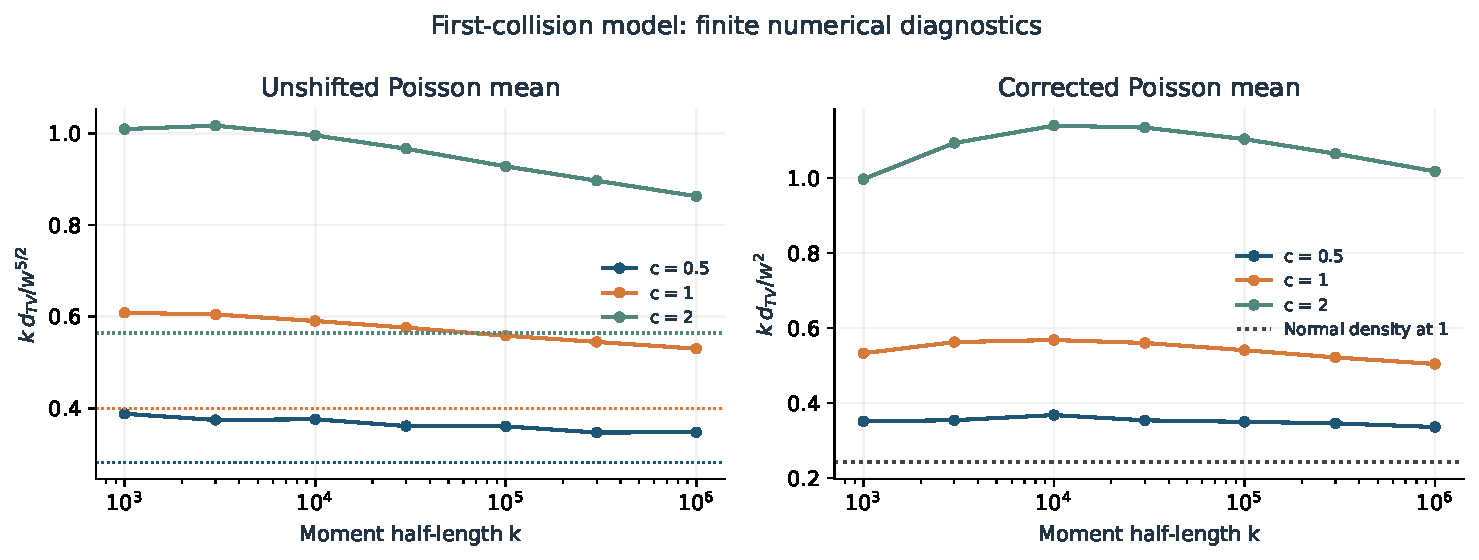
\includegraphics[width=\textwidth]{figures/06-meandeg-deficit_profiles.pdf}
 \caption{Scaled total variation diagnostics for the normalized
 first-collision model, at $c=1/2,1,2$. Left: comparison with
 $\Poi(cw)$, scaled by $k/w^{5/2}$. Right: comparison with
 $\Poi(cw+cw^3/k)$, scaled by $k/w^2$. The full walk law is controlled
 analytically in the proofs, not simulated by this plot.}
 \label{sgm:md:fig:deficit}
\end{figure}

For Figure~\ref{sgm:md:fig:critical}, set
\[
 w=\tfrac12\log(k/\tau),\qquad c=\frac{\sqrt{\tau k}}{w},
 \qquad \tau\in\{1/4,1/2,1,2\}.
\]
Then $c^2w^2/k=\tau$ holds exactly. The plotted quantity is the
fresh-law average of the exact Catalan quotient $Q(k,s)$ in its
concentrated window. It is the explicit term identified in the proof
of Theorem~\ref{sgm:md:gd:main}, and the horizontal lines are $e^\tau$.
The proof, not this numerical average, controls the omitted classes
of walks.

\begin{figure}[htbp]
 \centering
 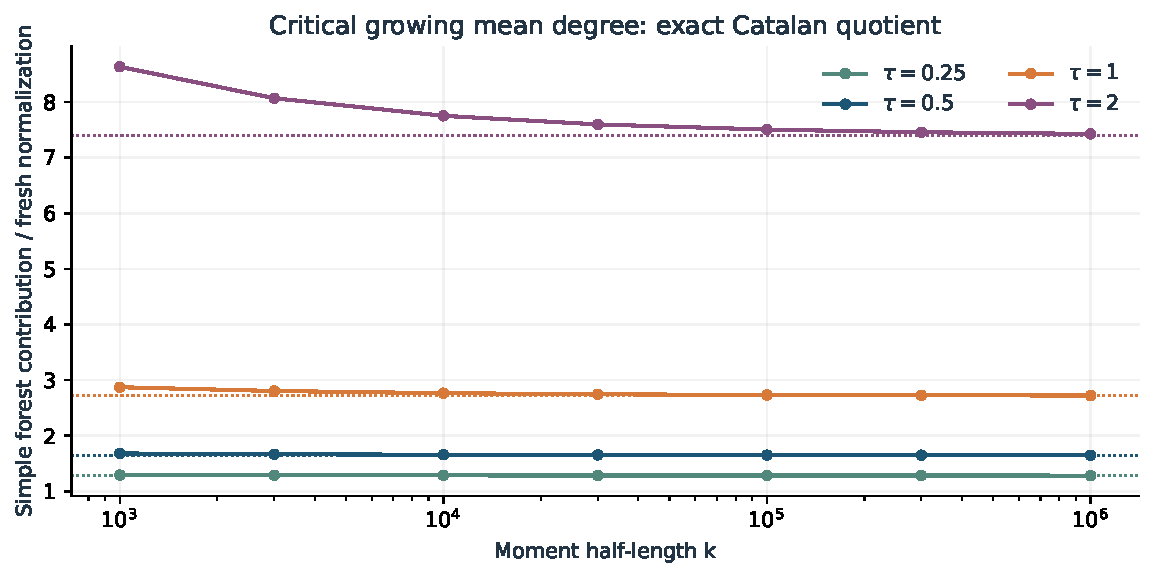
\includegraphics[width=0.95\textwidth]{figures/06-meandeg-critical_transition.pdf}
 \caption{Critical-window diagnostics for the simple-forest
 contribution. The numerical average of $Q(k,s)$ approaches the
 predicted factor $e^\tau$. The reported global error bound includes
 additional contributions that are not evaluated by this figure.}
 \label{sgm:md:fig:critical}
\end{figure}

The numerical program uses positive Dobi\'nski sums centered at the
Touchard saddle, with log-sum-exp arithmetic. Repeating the sums with
widths $12$ and $15$ saddle standard deviations, each with a
$20$-integer cushion, changes the computed fresh distribution by at
most $9.3\times10^{-15}$ in $\ell^1$ over the recorded cases.
This is a stability check, not an interval-arithmetic certificate of
all discarded tails or floating-point errors. The JSON files record
all $12$ finite-moment rows, $21$ deficit-model cases, and $28$
critical-window cases, with their scope written into the metadata.

\subsection{Reproduction and integration}

The ZIP contains the TeX source, the compiled PDF, all input sections,
the bibliography, the scripts, raw exact rows, verification summaries,
and vector and raster figures. A \texttt{README.md} gives the build
commands and a suggested report directory in the ProveIt repository.
The exact integer checks need only Python's standard library; symbolic
and numerical diagnostics additionally use SymPy, NumPy, SciPy, and
Matplotlib. The supplied dependency versions record the environment
used for the archived run. No external dataset or network call is
needed to rebuild the article or rerun the computations.

The claim ledger distinguishes proved results, inherited ingredients,
finite checks, illustrations, and open questions. The provenance file
pins the inspected repository revisions, and \texttt{source\_audit.txt}
records the source-access and priority boundaries. Integration can
therefore preserve both the mathematical statements and the evidence
supporting the scope of the novelty claim. No theorem-prover source
is included: the present deliverable is a research article with proofs
and reproducibility code.
\begin{writenote}[The package here, and the write's recomputation, 9 October 2026]
In this report the programs named above are
\file{code/06-meandeg-verify_exact.py},
\file{code/06-meandeg-verify_symbolic.py} and
\file{code/06-meandeg-numerical_diagnostics.py}; the data files are
\file{data/06-meandeg-*}, the figures \file{figures/06-meandeg-*}, the
claim ledger, provenance file and verification record
\file{data/06-meandeg-claim_ledger.json}, \file{data/06-meandeg-provenance.json}
and \file{data/06-meandeg-verification_report.json}, and
\file{source_audit.txt} is \file{06-meandeg-source_audit.txt}. The ZIP, the
compiled PDF, the section sources, the bibliography and the delivered
\file{README.md} are not shipped (Section~\ref{sgm:md:sec:provenance}). The
programs read and write the delivered names (\file{data/exact_rows.json} and so
on), so they run only on a copy with the delivered layout (the README gives
the recipe). With its own integer-scaled implementation of the first-child
recurrence, the write recomputed every scaled moment of
\file{data/06-meandeg-exact_rows.json} at $c=\frac12,1,2$ for $k\le128$ (all
equal) and all eighteen entries of Table~\ref{sgm:md:tab:finite-moments} (all
equal to the printed six decimals); with SymPy it recomputed the four
displayed polynomials, $d_4$ and $P_4$ (equal to the generated fragment
\file{data/06-meandeg-collision_polynomials.tex}). The two figures plot
explicitly labelled models (the first-collision law~\eqref{sgm:md:num:first-model}
and the fresh-law average of $Q(k,s)$), not the full walk law; they
illustrate, and were not recomputed.
\end{writenote}
% ---- end of 06_verification.tex ----
% ---- delivered sections/07_research.tex ----
\section{Further research questions and topics}
\label{sgm:md:sec:research}

The results leave several concrete problems. We separate improvements
to the present estimates from changes of regime or model; a result in
one category need not automatically supply a result in another. The
questions below are proposed projects, not conclusions established
by the current article.

\subsection{Sharper critical asymptotics and a wider parameter range}

\begin{question}[The first correction in the critical regime]\label{sgm:md:q:critcorr}
What is the first nonzero asymptotic correction to
$\log\{m_k(c)/(2H_k(c))\}-c^2w^2/k$ when $cw/\sqrt{k}$ stays bounded
away from zero and infinity?
\end{question}
The present $k^{-1/4}\log^{13/4}k$ bound is produced by a
coefficient-extraction penalty and a deliberately broad cutoff. It
does not identify the first neglected term. The exact expansion
\[
 \log Q(k,s)=\frac{s(s-1)}k
 +\frac{s^2(s-1)^2}{6k^3}+O(s^6/k^5)
\]
already separates the pure forest correction from repeated off-hub
edges. A sharper weighted allocation estimate, averaged over the
actual partition and deficit distributions instead of bounded by
their largest admissible values, is a natural route. The useful
output would be a uniform equivalent with an explicit correction
function of $u=cw/\sqrt{k}$.

\begin{question}[A uniform passage from bounded to growing mean degree]\label{sgm:md:q:uniform}
Can one obtain a single controlled expansion that joins compact
$c$ to the critical regime $cw\asymp\sqrt{k}$?
\end{question}
The quantities $cw^3/k$ and $c^2w^2/k$ measure different effects:
fixed-parameter collision corrections and the growth of fresh
planar interiors. Their relative size changes with $c$. The present
paper proves the two regimes separately; it does not establish a
uniform theorem throughout the intervening range. A successful
result should state the admissible range of $c$ explicitly and
bound the residual dependence on both quantities. Substituting
$c=c_k$ into an $O_K$ term is not a valid substitute for that task.

\begin{question}[Beyond the first critical window]\label{sgm:md:q:beyond}
For $cw/\sqrt{k}\to\infty$, how long does the Catalan quotient
continue to determine the leading logarithm of the full moment?
\end{question}
Higher terms in $\log Q$ become relevant as the deficit increases,
and the factor used to penalize repeated off-hub edges changes as
well. A larger-window saddle might still isolate a dominant vertex,
or a different geometry might become competitive. The main technical
target is a new complement estimate with matching logarithmic
precision, not simply an extrapolation of $e^{c^2w^2/k}$. The relation
to the large-mean, fixed-excess enumerations of
\cite{hdp} and the high-moment diluted-matrix regimes of
\cite{khor1} deserves a systematic comparison.

\begin{question}[Vanishing mean degree]\label{sgm:md:q:vanishing}
What replaces the compact-parameter expansion when $c=c_k\to0$?
\end{question}
The lower endpoint of the compact interval enters branch bounds
through inverse powers of $c$. Meanwhile $cw$ may remain bounded or
vanish, so the Gaussian limit used to evaluate the sharp Poisson
constants no longer applies. A useful classification would distinguish
$cw\to0$, $cw\to\lambda_0\in(0,\infty)$, and $cw\to\infty$,
and identify when walks using very few distinct edges become dominant.

\subsection{Probability laws and the geometry of contributing walks}

\begin{question}[Sharper positive approximations]\label{sgm:md:q:positive}
Can the positive two-jump compound Poisson approximation in
Corollary~\ref{sgm:md:dl:compound} be extended to the next asymptotic order,
with an optimal error constant in an explicitly specified family?
\end{question}
The signed quadratic correction explains why changing only the
Poisson mean has an irreducible error. Allowing a rare jump of size
two removes that term. At the next order, additional Charlier
coefficients must be identified together with sufficiently accurate
fresh-law estimates. A positive approximation imposes constraints
that a formal signed expansion does not. Determining the minimal
positive family capable of matching those coefficients is a
concrete approximation-theoretic problem.

\begin{question}[Local limits and moderate deviations at critical degree]\label{sgm:md:q:local}
What are the local limit law and the moderate-deviation range for
the dominant-vertex deficit when $cw\asymp\sqrt{k}$?
\end{question}
The present proof gives concentration and an $\ell^1$ comparison
after multiplying by $Q(k,s)$, but not a sharp pointwise law or
moderate-deviation expansion. A local theorem must track the
binomial mixture, the shifted Poisson saddle, and the Catalan tilt
on the same scale. Relative error in a shrinking tail probability
requires substantially more than the total-mass error used here.

\begin{question}[Joint hub statistics]\label{sgm:md:q:joint}
Can one determine the joint law of the departure deficit, the number
of distinct neighbors of the dominant vertex, its largest excursion
block, and the number and depths of off-hub edges?
\end{question}
Departure count and graph degree are different statistics. A joint
generating function with separate marks would quantify which
features create the correction terms. In the critical regime,
Corollary~\ref{sgm:md:gd:simpledominance} says that repeated off-hub edges
are rare in total weight, but it does not give a limiting law for
their number or locate the deepest fresh branch. Marked Catalan
forests and weighted block counts provide an exact starting point.

\begin{question}[Several competitive dominant vertices]\label{sgm:md:q:several}
Is there a parameter range in which configurations with two or more
heavily visited vertices contribute at leading order?
\end{question}
They are negligible in the two regimes proved here. Establishing
their onset, or proving a much larger exclusion range, would require
an optimization over weighted tree skeletons and excursion
allocations. A rigorous answer should compare the full combinatorial
weight, not just the adjacency spectral radius of a candidate tree.

\subsection{Finite graphs, other models, and verification}

\begin{question}[A simultaneous finite-graph transfer theorem]\label{sgm:md:q:finite}
For what explicit ranges of $k=k_N$ and $c=c_N$ do these tree-moment
equivalents approximate $N^{-1}\E\operatorname{Tr}A_{N,c}^{2k}$?
\end{question}
The fixed-$k$ limit in Proposition~\ref{sgm:md:def:graphmoment} is elementary,
but its error is not uniform in $k$. A transfer theorem must bound
non-tree normalized words, repeated graph-label assignments, and
their dependence on $c$. To reach statements about typical graphs,
one would then need concentration or higher trace moments. This is
an essential step before using the present formula as a finite-matrix
spectral estimate.

\begin{question}[Spectral tails from sharp moments]\label{sgm:md:q:tails}
What rigorous upper and lower bounds on the limiting spectral
measure can be recovered from the corrected moment growth?
\end{question}
Optimizing Markov's inequality gives a route to tail upper bounds,
but matching lower bounds and refined prefactors require additional
information. The sparse limiting measure can have atoms, so a
pointwise density equivalent is not automatically meaningful.
The single-defect spectral calculations of
\cite{SemerjianCugliandolo2002} and the earlier sparse-tail work
\cite{RodgersBray1988} motivate the question while leaving the
required rigorous inversion separate from the moment results.

\begin{question}[Weighted edges and other offspring laws]\label{sgm:md:q:weighted}
Which parts of the collision and forest analysis survive for
random edge weights, configuration models, or local weak limits
with a non-Poisson offspring distribution?
\end{question}
Random edge weights attach a moment depending on edge multiplicity,
so the single factor $c$ for each distinct edge is no longer
sufficient. A non-Poisson offspring law changes the weighted partition
structure and may change both the typical hub and its correction
scale. A useful theorem would state conditions on the weight moments
and offspring tails under which a dominant vertex still controls
the high moments, together with a replacement for the exact
Touchard normalizer. The weighted-graph moment framework of
\cite{Khorunzhy2004} is a natural point of comparison.

\begin{question}[Effective bounds and formal certification]\label{sgm:md:q:effective}
Can the arguments be converted into explicit finite-$k$ inequalities
and a machine-checked proof of the principal theorems?
\end{question}
There are two separate milestones. Effective analysis would replace
the unspecified constants and onset thresholds in the saddle,
collision, and complement estimates by usable values, ideally with
interval-certified diagnostics. Formalization could begin with the
finite combinatorial core: the weighted rotation identity including
periodic words, the first-child recurrence, the partition
decomposition, and the P\'olya factorial identities. A complete
proof-assistant development would also certify the
Bauer--Golinelli comparison, the uniform analytic estimates, and
the $\ell^1$ limit arguments. The exact code in this archive is a
regression resource for that effort, not a formal proof.

\subsection{Suggested order of attack}

The nearest extensions are the first critical correction, the
intermediate-parameter uniform theorem, and the next positive
probability approximation: all three can reuse the exact
decompositions in this article. Finite-graph transfer has a larger
combinatorial scope but would make the results more directly useful
for random matrices. Spectral inversion and general offspring laws
require additional ideas and should be treated as separate research
projects. Formal certification can proceed in parallel, beginning
with the identities that are already finite and exact.
% ---- end of 07_research.tex ----
\begin{writenote}[Further questions of Part~VI, 9 October 2026]
Following Vladimir Reshetnikov's standing rule of 4~October 2026, every claim
of the manuscript that is not proved in full is stated as an open question;
these twelve research questions are the manuscript's own, as delivered, and
the write labelled them. No claim of the manuscript was found wrong, and
nothing is moved or refuted. Relations to Section~\ref{sgm:sec:questions}:
Question~\ref{sgm:md:q:effective} is item~\ref{sgm:q:effective} for general
$c$; Questions~\ref{sgm:md:q:uniform} and~\ref{sgm:md:q:vanishing} are the
parts of item~\ref{sgm:q:meandegree} that Theorem~\ref{sgm:md:cm:main} leaves
open (a uniform passage from compact to growing $c$, and $c\to0$);
Question~\ref{sgm:md:q:tails} is close to item~\ref{sgm:q:spectral} (spectral
information from moments). Item~\ref{sgm:q:growing}, a growing collision
order, is none of these questions and stays open; the growing-degree
transition of Section~\ref{sgm:md:gd:section} is a different limit.
\end{writenote}
\begin{writenote}[Independent check of the Part~VI write, 9 October 2026]
An independent adversarial check of the Part~VI write (\file{cebf43994}) re-derived its
statements with its own code. \emph{The two consequences the write proved}, checked hardest.
(a)~Part~V's weighted bound: by $\binom ks=\binom{k-1}s+\binom{k-1}{s-1}$,
$H_k(c)=\sum_s\binom{k-1}sc^sT_{k-s}(c)+cH_{k-1}(c)$, so the right side
of~\eqref{sgm:sb:eq:weighted} at $\alpha=c$ is $2(H_k(c)-cH_{k-1}(c))-P_k(c)$
(exact for $k\le128$ at $c=\frac12,1,2$). Both Parts define the same moment
(the limiting normalized trace of the unscaled adjacency matrix of $G(N,c/N)$,
$\mu_{2k}(c)=m_k(c)$), and $cH_{k-1}/H_k\to0$ (log-convexity of the moments of $X+c$,
which is unbounded), $P_k$ grows at most geometrically by~\eqref{sgm:sb:eq:Pgf}
while $H_k$ grows faster than every geometric sequence, so with
Theorem~\ref{sgm:md:cm:main} at $K=\{c\}$ the bound is $\sim\mu_{2k}(c)$; as at $c=1$ the
approach is slow: the bound over $\mu_{2k}(c)$ is $0.749$, $0.627$, $0.438$ at $k=128$
for $c=\frac12,1,2$, and $cH_{k-1}/H_k$ there is $0.0161$, $0.0279$, $0.0472$, close to
$cw/k$. (b)~At $c=1$, Corollary~\ref{sgm:md:cm:explicit} gives
$M_{2k}/(2B_{k+1})=1+W^3/(2k)+2W^2/k+O(W^6/k^2)$ (here $W=W(k)$ is its $w$, and $H_k(1)=B_{k+1}$), and
Theorem~\ref{sgm:lw:thm:asympt} with~\eqref{sgm:lw:eq:Bellratio} gives
$G_k/(2B_{k+1})=1+(1+o(1))W^2/k$; as $W^6/k^2=o(W^2/k)$, subtraction gives the
write's $(M_{2k}-G_k)/(2B_{k+1})=W^3/(2k)+(1+o(1))W^2/k$. As finite illustrations only,
$[(M_{2k}-G_k)/(2B_{k+1})-W^3/(2k)]/(W^2/k)$ is $10.1$, $8.42$, $3.80$, $2.59$ at
$k=16,32,64,128$ (the omitted terms are of relative order $W^4/k$), and
$(G_k-2B_{k+1})/(2B_{k+1})$ over $W^2/k$ is $1.79$, $1.38$, $1.21$, $1.12$.
\emph{Recomputed by other routes}: $m_k(c)$ at $c=\frac12,1,2$ for $k\le128$ by an
excursion recurrence at the root (set partitions of the root excursions by child, an
exponential formula; not the first-child recurrence) in integers, equal to every scaled
moment of \file{data/06-meandeg-exact_rows.json}, to a brute-force enumeration for
$k\le7$ and to the 13 terms of A094149 (revision \#10 of 13~July 2025, read again);
$m_1,\dots,m_5$ as polynomials in $c$; all eighteen entries of
Table~\ref{sgm:md:tab:finite-moments}; $A_1(k,1)=T_k/B_{k+1}$ for $3\le k\le60$ (an
identity term by term) and $(A_1-P_1)/(w^4/k^2)$ at $k=20,40,60$ for the three $c$;
$F(t)$ against quadrature at five points, $F(0)=\varphi(1)$, $\E C_2(Y;u)^2=2u^2$,
$\operatorname{Var}(Y)_2=4u^3+2u^2$, $\E|Y-\lambda|=2\lambda\pi_\lambda(\lfloor\lambda\rfloor)$
at $\lambda=3.7$, $25.2$, $400.5$; $\log Q(k,s)$ to third order. Also confirmed: the
archive (2{,}095{,}612 bytes, 33 files, 3{,}896{,}295 bytes unpacked), the 23
byte-identical staged files, the pin \file{9570aaede2} and the blob \file{f6a72e04cf}
at the pin and before the write, the numbering (324 earlier labels unchanged, 158
delivered labels at section $+57$ with Table~1 as Table~\ref{sgm:md:tab:finite-moments},
19 added, 501 in all), the 192 references (144 + 48), and the README's 106 files.
No claim of Part~VI or of the write was found wrong.
\end{writenote}

\begin{thebibliography}{99}\raggedright
\bibitem{bg} Michel Bauer and Olivier Golinelli.
\emph{Random incidence matrices: moments of the spectral density}.
Journal of Statistical Physics \textbf{103} (2001), 301--337.
\href{https://doi.org/10.1023/A:1004879905284}{doi:10.1023/A:1004879905284}.
Primary preprint: \href{https://arxiv.org/abs/cond-mat/0007127v2}{arXiv:cond-mat/0007127v2}.
[All five Parts. Report~210 calls the preprint the ``primary full text''; Report~209 checked the full preprint \href{https://arxiv.org/pdf/cond-mat/0007127v2}{arXiv:cond-mat/0007127v2}, ``especially \S\S5.3--5.6''. Part~VI (key \texttt{BauerGolinelli2001}) cites \url{https://arxiv.org/abs/cond-mat/0007127}: ``The coefficientwise bound used here is Section~5.5, equation~(9), of the primary preprint.'']
\bibitem{kv} A. Khorunzhy and V. Vengerovsky.
\emph{On asymptotic solvability of random graph's laplacians}.
\href{https://arxiv.org/abs/math-ph/0009028}{arXiv:math-ph/0009028} (2000). [Part~I.]
\bibitem{spiridonov} Alexey Spiridonov.
\emph{Spectra of sparse graphs and matrices}. Senior thesis.
\href{https://alexey.im/papers/sparse-random-graphs-senior-thesis.pdf}{Author-hosted primary text}.
[Part~I; Report~209 cites it as ``senior thesis on sparse random graphs, author-hosted PDF, especially \S3.3'', \url{https://alexey.im/papers/sparse-random-graphs-senior-thesis.pdf}.]
\bibitem{hdp} Eva-Maria Hainzl and \'Elie de Panafieu.
\emph{Tree walks and the spectrum of random graphs}.
\href{https://arxiv.org/abs/2405.08347v1}{arXiv:2405.08347v1} (14 May 2024).
Conference version: LIPIcs AofA 2024, Article 11, \href{https://doi.org/10.4230/LIPIcs.AofA.2024.11}{doi:10.4230/LIPIcs.AofA.2024.11}.
Journal record: European Journal of Combinatorics \textbf{136} (2026), 104386, \href{https://doi.org/10.1016/j.ejc.2026.104386}{doi:10.1016/j.ejc.2026.104386}.
[All five Parts; Reports~212 and~210 omit the journal record; Report~209 cites the full preprint as \href{https://arxiv.org/abs/2405.08347}{arXiv:2405.08347} (2024) and adds ``Journal full text not independently accessed''; the date 14 May 2024 is Report~210's, and the journal's name, volume and article number are Report~209's. Part~VI (key \texttt{Hainzl2024}) cites the journal record first, with the preprint (2024) and the conference version.]
\bibitem{hainzl} Eva-Maria Hainzl.
\emph{Formulas and asymptotics of hypergraph Catalan numbers}.
\href{https://arxiv.org/abs/2508.08865v2}{arXiv:2508.08865v2}, 23 March 2026.
[Part~I. Report~209 cites \href{https://arxiv.org/abs/2508.08865}{arXiv:2508.08865} (2025) with the conference version \href{https://doi.org/10.4230/LIPIcs.AofA.2026.20}{doi:10.4230/LIPIcs.AofA.2026.20}, ``Fixed-multiplicity scope checked''.]
\bibitem{jjs} Svante Janson, Thordur Jonsson, and Sigurdur O. Stef\'ansson.
\emph{Random trees with superexponential branching weights}.
\href{https://arxiv.org/abs/1104.2810}{arXiv:1104.2810} (2011).
\href{https://doi.org/10.1088/1751-8113/44/48/485002}{doi:10.1088/1751-8113/44/48/485002}. [Parts~I and~II; the DOI is Report~214's.]
\bibitem{janson} Svante Janson.
\emph{Simply generated trees, conditioned Galton--Watson trees, random allocations and condensation}.
Probability Surveys \textbf{9} (2012), 103--252.
\href{https://doi.org/10.1214/11-PS188}{doi:10.1214/11-PS188}.
\href{https://arxiv.org/abs/1112.0510}{arXiv:1112.0510} (2011). [Part~I cites the journal, Part~II the preprint.]
\bibitem{r213} \emph{The full sparse graph moment equivalent}.
Report213, 4 October 2026. Companion report, circulated as a PDF and reproducibility package.
The required complement theorem is recalled with proof in Appendix~\ref{sgm:co:sec:complement} here.
[Part~I. Printed in this report as Part~II.]
\bibitem{hm} Ella Hiesmayr and Theo McKenzie.
\emph{The Spectral Edge of Constant Degree Erd\H{o}s--R\'enyi Graphs}.
\href{https://arxiv.org/abs/2309.11007}{arXiv:2309.11007} (2023).
Random Structures \& Algorithms \textbf{66} (2025), e70011,
\href{https://doi.org/10.1002/rsa.70011}{doi:10.1002/rsa.70011}. [Parts~II and~III; the year of the preprint is Report~212's.]
\bibitem{bbg} Bhaswar B. Bhattacharya, Sohom Bhattacharya, and Shirshendu Ganguly.
\emph{Spectral Edge in Sparse Random Graphs: Upper and Lower Tail Large Deviations}.
\href{https://arxiv.org/abs/2004.00611}{arXiv:2004.00611}. [Part~III.]
\bibitem{ablo} Louigi Addario-Berry, G\'abor Lugosi, and Roberto Imbuzeiro Oliveira.
\emph{The top eigenvalue of uniformly random trees}.
\href{https://arxiv.org/abs/2403.08443v2}{arXiv:2403.08443v2}. [Part~III.]
\bibitem{hmt} Markus Heydenreich, Peter M\"uller, and Sara Terveer.
\emph{Return probability on Bienaym\'e--Galton--Watson trees and spectral asymptotics of sparse Erd\H{o}s--R\'enyi random graphs}.
\href{https://arxiv.org/abs/2603.00344v2}{arXiv:2603.00344v2} (21 July 2026). [Part~III.]
\bibitem{bordenave} Charles Bordenave.
\emph{Sparse graphs and their Benjamini--Schramm limits: a spectral tour}.
\href{https://arxiv.org/abs/2510.10299}{arXiv:2510.10299}. [Part~III.]
\bibitem{valigi} P. Valigi, J. W. Baron, I. Neri, G. Biroli, and C. Cammarota, \emph{Eigenvalue spectral tails and localization properties of asymmetric networks}, Journal of Physics A \textbf{58} (2025), 455002. \href{https://doi.org/10.1088/1751-8121/ae16ec}{doi:10.1088/1751-8121/ae16ec}; \href{https://arxiv.org/abs/2507.20225}{arXiv:2507.20225}. Selected full-text sections checked. [Part~V.]
\bibitem{khor1} O. Khorunzhiy, \emph{On high moments of strongly diluted large Wigner random matrices}, \href{https://arxiv.org/abs/1311.7021}{arXiv:1311.7021}. Abstract-level regime check only. [Part~V. Part~VI (key \texttt{Khorunzhiy2016}) cites it as S\'eminaire de Probabilit\'es XLVIII, Lecture Notes in Mathematics \textbf{2168}, Springer, 2016, pp.~347--399.]
\bibitem{khor2} O. Khorunzhiy, \emph{On asymptotic properties of high moments of compound Poisson distribution}, \href{https://arxiv.org/abs/2007.00379}{arXiv:2007.00379}. Abstract-level scope check only. [Part~V.]
\bibitem{oeis} OEIS Foundation Inc.
\emph{The On-Line Encyclopedia of Integer Sequences},
\href{https://oeis.org/A094149}{A094149}, contributed by Alexey Spiridonov.
[All five Parts, each checked on 4 October 2026: ``Positive-order normalization checked'' (Report~214); ``Sequence identity and positive-order terms checked'' (Reports~213, 212, 210); ``Identification and 13-term prefix checked'' (Report~209, which cites the entry as The OEIS Foundation, \emph{A094149}, \url{https://oeis.org/A094149}). Read by the write on 7 October 2026 at revision \#10 of 13 July 2025 (Remark~\ref{sgm:co:rem:oeis}). Part~VI (key \texttt{OEISA094149}): ``original submission by A.~Spiridonov, 4~May 2004'', accessed 8~October 2026; read again at its write, 9~October 2026: revision \#10, unchanged.]
\bibitem{TSvol} ProveIt, \emph{Transseries and inversion}, \file{Analysis/Transseries/docs/series-and-transseries/Transseries_And_Inversion/transseries_and_inversion.tex}; Part~0 (\file{p0:def:model}, \file{p0:def:three-inverses}, \file{p0:thm:staircase}, \file{p0:thm:lambert-core}, \file{p0:thm:lambert-centered}), \file{plt:thm:lw-template}, and the Bell chapter \file{q2:sec:bell}. [Added in the write.]
\bibitem{Khorunzhy2004} O. Khorunzhy, M. Shcherbina, and V. Vengerovsky.
\emph{Eigenvalue distribution of large weighted random graphs}.
Journal of Mathematical Physics \textbf{45} (2004), 1648--1672.
\href{https://doi.org/10.1063/1.1667610}{doi:10.1063/1.1667610}.
Author copy: \url{https://ilt.kharkiv.ua/bvi/structure/depart_e/d24/rm_10.pdf}. [Part~VI.]
\bibitem{Khorunzhiy2020} O. Khorunzhiy.
\emph{On asymptotic properties of Bell polynomials and concentration of vertex degree of large random graphs}.
Journal of Theoretical Probability \textbf{35} (2022), 20--51; published online 4~October 2020.
\href{https://doi.org/10.1007/s10959-020-01025-w}{doi:10.1007/s10959-020-01025-w}.
Primary preprint: \href{https://arxiv.org/abs/1904.01339}{arXiv:1904.01339}. [Part~VI.]
\bibitem{Pittel1997} B. Pittel.
\emph{Random set partitions: asymptotics of subset counts}.
Journal of Combinatorial Theory, Series A \textbf{79} (1997), 326--359.
\href{https://doi.org/10.1006/jcta.1997.2791}{doi:10.1006/jcta.1997.2791}. [Part~VI.]
\bibitem{ArratiaGoldsteinGordon1990} R. Arratia, L. Goldstein, and L. Gordon.
\emph{Poisson approximation and the Chen--Stein method}.
Statistical Science \textbf{5} (1990), 403--434.
Author copy: \url{https://dornsife.usc.edu/larry-goldstein/wp-content/uploads/sites/221/2023/06/pacs-1.pdf}. [Part~VI; listed, not cited in its text.]
\bibitem{SemerjianCugliandolo2002} G. Semerjian and L. F. Cugliandolo.
\emph{Sparse random matrices: the eigenvalue spectrum revisited}.
Journal of Physics A: Mathematical and General \textbf{35} (2002), 4837--4851.
\href{https://doi.org/10.1088/0305-4470/35/23/303}{doi:10.1088/0305-4470/35/23/303};
\href{https://arxiv.org/abs/cond-mat/0202406}{arXiv:cond-mat/0202406}. [Part~VI.]
\bibitem{RodgersBray1988} G. J. Rodgers and A. J. Bray.
\emph{Density of states of a sparse random matrix}.
Physical Review B \textbf{37} (1988), 3557--3562.
\href{https://doi.org/10.1103/PhysRevB.37.3557}{doi:10.1103/PhysRevB.37.3557}. [Part~VI; Part~I names it in its sources without an entry.]
\bibitem{ProveIt2026} ProveIt repository.
\emph{Sparse graph moments: closed tree walks (OEIS A094149)}, merged research report comprising
Reports~214, 213, 212, 210, and~209; reports dated 4~October 2026, merged 7~October 2026.
Unrefereed research manuscript; snapshot \texttt{9570aaede2458830be9b3bbb072481c88f4f5a4c}.
[Part~VI. This report's Parts~I--V, unchanged at the snapshot.]
\bibitem{OpenAIMath2026} OpenAI.
\emph{openai/math: research manuscript repository}, snapshot
\texttt{adc7f1241b42e322a6451854ab7e4b4c146bf78a}, accessed 8~October 2026.
\url{https://github.com/openai/math/tree/adc7f1241b42e322a6451854ab7e4b4c146bf78a}.
Repository context only. [Part~VI; not checked by the write.]
\end{thebibliography}
\end{document}
